\documentclass[pdflatex,sn-mathphys-num]{sn-jnl} % Math and Physical Sciences Numbered Reference Style
\usepackage{amsmath,amssymb,amsfonts}
\usepackage{graphicx}
\usepackage{hyperref}
\usepackage{physics}
\usepackage{tikz}
\usepackage{amsopn}
\usepackage{amstext}
\usepackage{microtype}
\usepackage{xparse}
\NewDocumentCommand{\subsubsubsection}{s m}{%
  \IfBooleanTF{#1}{\paragraph*{#2}}{\paragraph{#2}}%
}
\usetikzlibrary{arrows.meta, calc, decorations.pathmorphing, shapes.geometric, shadings, positioning, decorations.markings}

\title[Cosmochrony]{Cosmochrony: An Exploratory Geometric Framework for Emergent Spacetime, Gravitation, and Quantum Phenomena}
\author*[1]{\fnm{Jérôme} \sur{Beau}}\email{javarome@gmail.com}
\affil*[1]{\orgname{Independent Researcher}, \country{France}}
\date{}

\abstract{
  We propose \emph{Cosmochrony}, a foundational physical framework in which time, inertia,
  and spacetime geometry emerge from the irreversible relaxation of a single fundamental
  scalar field~$\chi$.
  Unlike conventional field theories defined on a pre-existing spacetime,
  Cosmochrony treats relaxation as the primary physical process, from which
  temporal ordering, effective metrics, and dynamical laws arise.

  Localized, long-lived excitations of the $\chi$ field appear as topologically
  and spectrally stable solitonic configurations.
  Their inertial mass is not postulated but emerges as a measure of resistance
  to global relaxation, quantified by the internal curvature and stability spectrum
  of the configuration.
  In regimes where an effective relativistic description applies, this interpretation
  naturally reproduces $E = mc^2$ as a kinematic identity rather than a fundamental axiom.
  Spin, statistics, and fermionic $4\pi$ periodicity originate from topological
  obstructions in the configuration space of $\chi$ excitations.

  An effective spacetime metric arises through coarse-grained projections of $\chi$
  relaxation dynamics, avoiding the assumption of a fundamental geometry.
  Gravitational and electromagnetic interactions are interpreted as manifestations
  of relaxation gradients and deformations of the underlying field, while gravitational
  waves correspond to propagating modulations of $\chi$.
  The Higgs mechanism is recovered as an effective low-energy description of how
  localized excitations acquire inertial properties within an already structured
  relaxation background, without modifying its empirical phenomenology.

  At cosmological scales, the framework provides a unified interpretation of cosmic
  expansion, dark matter, and dark energy in terms of the global relaxation budget
  of the $\chi$ field.
  The observed Hubble tension is addressed through nonlinear relaxation effects,
  without invoking new particle species or inflationary dynamics.

  Cosmochrony does not aim to replace the Standard Model or General Relativity at
  accessible energies, but to supply a deeper explanatory layer in which their
  structures emerge from a common physical origin.
  The framework yields testable qualitative predictions, identifies clear numerical
  programs for validation via lattice simulations, and delineates the conditions
  under which effective field theories and spacetime descriptions remain valid.
}

\keywords{Emergent spacetime, quantum gravity, cosmology, geometric frameworks}

\begin{document}
  \maketitle

  \tableofcontents

  \clearpage

\section{Introduction}
  \label{sec:introduction}

  Modern fundamental physics is built upon two highly successful yet conceptually
  distinct frameworks: quantum mechanics and general relativity~\cite{Dirac1930,Einstein1915}.
  Quantum theory accurately describes microscopic phenomena, while general
  relativity provides a geometric account of gravitation and spacetime dynamics
  at macroscopic and cosmological scales.
  Despite their empirical success, these theories rely on incompatible foundational
  assumptions and resist unification within a single coherent conceptual
  framework~\cite{MisnerThorneWheeler1973,Weinberg1972,rovelli2004quantum}.

  Quantum mechanics presupposes a fixed spacetime arena in which physical states
  evolve, whereas general relativity identifies spacetime geometry itself as a
  dynamical entity.
  Numerous approaches have attempted to bridge this tension, including quantum
  field theory in curved spacetime, canonical and covariant quantum gravity
  programs, and string-based or holographic frameworks.
  While these approaches have led to important theoretical developments, they
  typically rely on extended mathematical structures or introduce additional
  degrees of freedom whose physical interpretation and empirical accessibility
  remain unclear.

  In this work, we explore a complementary and deliberately minimalist framework,
  referred to as \emph{Cosmochrony}\footnote{From \textit{$\kappa\acute{o}\sigma\mu o\varsigma$} and
\textit{$\chi\rho\acute{o}\nu o\varsigma$}, denoting a framework in which cosmic structure
and temporal ordering emerge from a common pre-geometric substrate.}.
  The guiding hypothesis is that spacetime geometry, gravitation, and quantum
  phenomena emerge from the dynamics of a single continuous underlying entity,
  denoted $\chi$, whose effective descriptions arise through a constrained
  projection process.
  This projection is generically non-injective, allowing distinct underlying
  $\chi$-configurations to correspond to identical effective observables and,
  conversely, allowing a single underlying configuration to admit multiple
  correlated effective realizations.
  A detailed and formal treatment of this projection asymmetry is given in
  Section~\ref{subsec:projection-reality-and-ontological-asymmetry}.

  The substrate $\chi$ is not defined on a pre-existing spacetime manifold, nor is
  it interpreted as a conventional physical field propagating within spacetime.
  Instead, spacetime notions themselves arise as effective and relational
  descriptions, applicable only once suitable stability and projection conditions
  are satisfied.
  The precise ontological status of $\chi$ and the minimal assumptions governing
  its dynamics are introduced systematically in
  Section~\ref{sec:definition-and-fundamental-properties-of-the-chi-field}.

  The fundamental dynamical postulate of Cosmochrony is that $\chi$ undergoes an
  irreversible relaxation process, locally bounded by an invariant structural
  propagation speed.
  The effective projection of this bound defines the observed causal limit $c$ and
  induces an intrinsic ordering of physical processes, identified with physical
  time.
  Spatial relations emerge relationally from differences, gradients, and
  correlations of $\chi$ once a stable geometric regime is reached.
  Within this perspective, spacetime expansion, gravitation, particle-like
  excitations, radiation processes, and quantum correlations are not fundamental
  ingredients, but emergent phenomena associated with specific configurations or
  interactions of the underlying substrate.
  In particular, discreteness, inertial mass, and quantum indeterminacy are shown
  later to arise from structural constraints on projection and relaxation, rather
  than from independent postulates.

  Cosmochrony does not aim to replace the Standard Model or general relativity in
  their empirically validated domains, nor does it claim to provide a final
  unification of quantum theory and gravitation.
  Instead, it offers an exploratory and internally coherent framework designed to
  clarify the physical origin of time, geometry, gravitation, and quantum
  correlations within a single relational dynamics.
  Standard geometric and quantum formalisms are recovered only at an effective,
  coarse-grained level, applicable when $\chi$ admits a stable spacetime
  interpretation.

  Accordingly, quantities such as coordinates, metric structure, variational
  principles, and differential geometry are not treated as fundamental.
  They are employed later in the paper as emergent descriptive tools, rather than
  as primary postulates of the theory.
  Technical reconstructions and mathematical details are therefore confined to the
  appropriate effective regimes and collected in the appendices.

  The unifying thread of the framework is the idea that apparent multiplicity,
  indeterminacy, and nonlocality reflect structural features of projection, rather
  than fundamental physical randomness or superluminal dynamics.

  The structure of the paper is as follows.
  Sections~2--4 introduce the conceptual motivations and minimal dynamical
  assumptions governing the $\chi$ substrate.
  Subsequent sections examine how particle-like excitations, gravitation, quantum
  correlations, and cosmological behavior emerge in appropriate regimes.

  \subsection{Conceptual Context and Related Approaches}
  \label{subsec:conceptual-context-and-related-approaches}

  The idea that spacetime geometry and gravitation may be emergent rather than fundamental
  has been explored in a variety of contemporary theoretical frameworks.
  Several approaches interpret the spacetime metric as an effective description arising from
  deeper geometric, informational, or dynamical structures, and recast gravitation as a
  collective or emergent phenomenon rather than as a fundamental interaction~\cite{Nye2024,Singh2025}.

  Cosmochrony belongs to this broad conceptual lineage, while adopting a deliberately minimalist ontological stance.
  Rather than postulating multiple underlying structures or microscopic degrees of freedom,
  it assumes a single pre-geometric relational substrate, denoted $\chi$, whose irreversible
  relaxation governs the emergence of physical observables.

  Like Loop Quantum Gravity (LQG), Cosmochrony holds that spacetime geometry is not
  fundamental~\cite{Rovelli2004}.
  However, the two frameworks operate at distinct conceptual and ontological levels.

  LQG provides a quantized description of geometry once a spacetime structure is already
  assumed, encoding areas and volumes through spin networks and holonomies.
  In this sense, it addresses the quantization of geometric degrees of freedom defined on a
  kinematical spacetime arena.

  Cosmochrony, by contrast, addresses an earlier and more primitive level.
  It does not quantize geometry, but seeks to explain how geometric notions themselves arise
  as effective, coarse-grained descriptions of underlying $\chi$-configurations.
  The emergence of spacetime is mediated by a non-injective projection from the pre-geometric
  substrate to effective observables, allowing geometric, dynamical, and quantum features to
  appear only once specific relational and spectral conditions are met.

  From this perspective, Cosmochrony does not compete with LQG but conceptually precedes it.
  It aims to account for the physical origin of the geometric degrees of freedom that may
  subsequently be quantized within approaches such as LQG, while remaining agnostic about
  the detailed form of their quantization at the effective level.


  For convenience, a glossary summarizing the main quantities and operators used
  throughout the article is provided in Appendix~\ref{appendix:glossary}.

  \clearpage
\section{Theoretical Context and Motivation}
  \label{sec:theoretical-context-and-motivation}

  \subsection{Conceptual Tension Between Quantum Theory and Gravitation}
  \label{subsec:conceptual-tension-between-quantum-theory-and-gravitation}

  Quantum mechanics and general relativity differ not only in their mathematical
  formalisms, but also in their foundational concepts.
  Quantum theory is intrinsically probabilistic, relies on a fixed causal structure,
  and treats time as an external parameter~\cite{Dirac1930,Born1926}.
  General relativity, by contrast, describes gravitation as the dynamics of spacetime
  geometry itself, with time acquiring a coordinate-dependent and observer-relative
  status~\cite{Einstein1915,MisnerThorneWheeler1973}.

  This conceptual mismatch becomes particularly acute in regimes where both quantum
  effects and strong gravitational fields are expected to be relevant, such as near
  spacetime singularities or in the early universe~\cite{penrose1989emperors,Prigogine1997}.
  Direct attempts to quantize gravity encounter persistent difficulties, including
  the problem of time, non-renormalizability, and the absence of a preferred background structure.
  These difficulties suggest that the tension may reflect not merely technical
  obstacles, but a deeper incompatibility in the assumed ontological status of time and geometry.

  \subsection{Limitations of Existing Unification Approaches}
  \label{subsec:limitations-of-existing-unification-approaches}

  Several major research programs have sought to address these challenges.
  Quantum field theory in curved spacetime successfully accounts for particle creation
  and vacuum effects, but retains a classical spacetime background~\cite{weinberg1972gravitation}.
  Canonical and covariant approaches to quantum gravity attempt to quantize spacetime
  geometry itself, often at the cost of substantial mathematical complexity and
  interpretational ambiguity.

  String theory and related frameworks introduce extended fundamental objects and
  higher-dimensional structures, offering deep mathematical unification but leading
  to a large space of possible low-energy realizations~\cite{rovelli2004quantum}.
  While internally rich, these approaches face ongoing challenges concerning empirical
  testability and the physical interpretation of their fundamental degrees of freedom.

  Collectively, these limitations motivate the exploration of alternative perspectives
  in which spacetime geometry, matter, and quantum behavior are not independently
  postulated, but emerge from a common underlying mechanism operating at a more
  primitive, pre-geometric level.

  \subsection{Minimalism as a Guiding Principle}
  \label{subsec:minimalism-as-a-guiding-principle}

  The framework developed in this work adopts minimalism as a guiding principle.
  Rather than introducing multiple fundamental fields, additional dimensions, or
  independent quantization rules, we explore whether a single continuous fundamental
  entity can account for temporal ordering, spatial relations, and quantum features
  within a unified relational dynamics.

  The scalar quantity $\chi$ is not interpreted as a conventional matter field, nor
  as a component of spacetime geometry.
  Instead, it represents a pre-geometric substrate whose irreversible relaxation
  underlies the emergence of both duration and separation.
  In this view, time and space are not independent primitives, but complementary
  aspects of a single dynamical process.
  Effective geometric and quantum descriptions arise only through coarse-grained,
  generally non-injective projections of the underlying $\chi$-configurations.

  \subsection{Time, Irreversibility, and Cosmological Expansion}
  \label{subsec:time-irreversibility-and-cosmological-expansion}

  A central motivation for the Cosmochrony framework is the close connection between
  time, irreversibility, and cosmological expansion.
  In standard cosmology, expansion is described kinematically through the scale factor,
  while the arrow of time is typically attributed to boundary conditions or entropy
  growth~\cite{peebles1993principles,Prigogine1997,penrose1989emperors}.

  In Cosmochrony, the monotonic relaxation of $\chi$ provides a unified origin for both phenomena.
  Irreversibility follows directly from the intrinsic directionality of the relaxation
  process, while cosmological expansion is interpreted as its large-scale geometric
  manifestation in the effective, projected description.
  From this perspective, expansion does not require an externally imposed energy
  component, but arises as an emergent consequence of the underlying pre-geometric dynamics.

  \subsection{Scope and Limitations}
  \label{subsec:context-and-motivation-scope-and-limitations}

  The aim of this work is exploratory rather than definitive.
  Cosmochrony does not seek to replace established theories within their empirically
  validated domains, but to offer a coherent reinterpretation that may clarify
  persistent conceptual difficulties concerning time, geometry, and quantization.

  Throughout the paper, emphasis is placed on internal consistency, conceptual clarity,
  and qualitative contact with observable phenomena, while openly acknowledging open questions and limitations.
  In the following section, we introduce the $\chi$ substrate formally and specify the
  minimal assumptions underlying its relational and dynamical structure.


  \clearpage
\section{Definition and Fundamental Properties of the \texorpdfstring{$\chi$}{χ} Substrate}
  \label{sec:definition-and-fundamental-properties-of-the-chi-field}

  Having outlined the conceptual motivations underlying Cosmochrony, we now introduce
  the single fundamental entity at the core of the framework.
  This section provides the \emph{canonical ontological definition} of the pre-geometric
  relational substrate $\chi$, which constitutes the primitive basis from which effective
  notions of spacetime, dynamics, and physical observables emerge.

  The aim of this section is to identify the \emph{minimal structural properties}
  required of $\chi$ for such effective descriptions to arise in appropriate regimes.
  No spacetime manifold, metric structure, or background geometry is assumed at this
  level.
  Instead, geometric and dynamical notions are recovered only through non-injective,
  coarse-grained projections of $\chi$ configurations once suitable stability conditions
  are met.
  This minimality principle, referred to throughout the paper as a regime of
  \emph{ontological poverty}, is adopted here as a foundational constraint rather than
  as a derived result.

  Throughout this section, the use of variational principles, Lagrangian formulations,
  or metric-based expressions does not imply that spacetime or a four-dimensional
  manifold is fundamental.
  Such formalisms are introduced strictly as effective descriptive tools, valid only in
  projectable regimes where configurations of $\chi$ admit a quasi-stable geometric and
  causal interpretation.
  They should therefore be understood as post-hoc representations of underlying
  pre-geometric dynamics, not as primary postulates of the theory.

  We begin by introducing the unified conceptual definition of the $\chi$ substrate and
  its physical interpretation, emphasizing its ontological distinction from conventional
  fields.
  The subsequent subsections progressively introduce more structured effective
  descriptions—including scalar, Lagrangian, and metric formulations—which become
  applicable only once projected $\chi$ configurations support a coherent spacetime
  regime.

  \subsection{Definition of the $\chi$ Field}
  \label{subsec:definition-of-the-chi-field}

  We postulate the existence of a single pre-geometric relational substrate, denoted $\chi$,
  which constitutes the primitive substrate of physical reality.
  The quantity $\chi$ is not defined on a pre-existing spacetime manifold and does not
  presuppose any metric, causal, or geometric structure.
  Instead, spacetime notions arise only as effective descriptions of the relational
  and dynamical properties of $\chi$ configurations.

  Ontologically, $\chi$ is not a scalar order parameter and does not possess values.
  Scalar order parameters arise only at the effective level, as coarse-grained descriptors of projected $\chi$
  configurations once a geometric regime is established.
  Dimensional quantities associated with length or time arise only at the effective level, once $\chi$
  configurations admit a geometric interpretation.
  The monotonic ordering intrinsic to $\chi$
  configurations gives rise, upon projection, to what is operationally perceived
  as temporal flow.

  Temporal ordering emerges from the global, monotonic ordering intrinsic to $\chi$ configurations across physical
  processes, establishing an intrinsic arrow of time without reference to an external temporal coordinate.
  Spatial separation, in turn, arises from relational differences between $\chi$
  configurations, giving rise to an effective notion of distance once a stable geometric
  regime is established.
  In this sense, time corresponds to ordering, while space corresponds to relational
  structure.

  At no stage is $\chi$ interpreted as a spacetime coordinate or as a material field
  propagating on spacetime.
  Spacetime coordinates and metric structure appear only as secondary, coarse-grained
  constructs, becoming meaningful when $\chi$ configurations admit a quasi-stable
  geometric interpretation.
  The spacetime metric thus functions as an emergent, effective descriptor of resistance
  to $\chi$ relaxation\footnote{The term ``relaxation'' is used here in a geometric and
  dynamical sense, and should not be confused with thermodynamic relaxation processes
  involving dissipation or entropy increase.} and of the propagation of perturbations
  within the field.

  The analogy with thermodynamic order parameters applies only at the effective level: $\chi$ itself is not an order
  parameter, but gives rise to effective order parameters once projected.
  In the Cosmochrony framework, $\chi$ therefore provides the minimal ontological basis
  from which time, space, gravitation, and quantum phenomena jointly emerge.

  In the following sections, spacetime coordinates and metric quantities will be
  introduced strictly as effective tools, valid in regimes where $\chi$ admits a stable
  geometric interpretation.

  \begin{figure}[h]
    \centering
    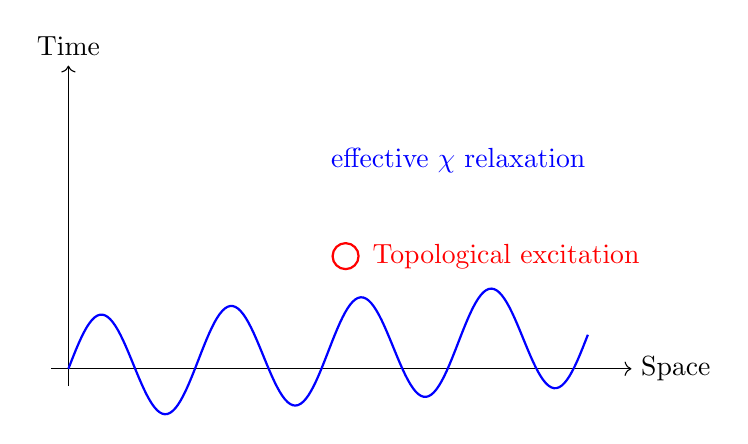
\begin{tikzpicture}[scale=1.1]

% Axes
      \draw[->] (-0.2,0) -- (6.5,0) node[right]{Space};
      \draw[->] (0,-0.2) -- (0,3.5) node[above]{Time};

% Wave
      \draw[thick, blue, domain=0:6, samples=200]
      plot (\x,{0.6*sin(2*pi*\x/1.5 r) + 0.4*\x/6});

% Particle crest
      \draw[red, thick] (3.2,1.3) circle (0.15);
      \node[red, right] at (3.4,1.3) {Topological excitation};

% Annotation
      \node[blue] at (4.5,2.4) {effective $\chi$ relaxation};

    \end{tikzpicture}
    \caption{Conceptual representation of Cosmochrony.
    An effective spacetime depiction of the projected scalar description of $\chi$,
      used for visualization purposes only.
      The monotonic relaxation of $\chi$ gives rise to an effective temporal ordering,
      while localized topological excitations correspond to particle-like configurations
      in the emergent geometric regime.}
    \label{fig:chi_concept}
  \end{figure}

  \paragraph{On the use of spacetime language.}
    Throughout this work, phrases such as ``spacetime coordinates,'' ``metric tensor,'' and ``four-dimensional
    manifold'' appear frequently, for the sake of clarity and effective description.
    These should be understood as \emph{emergent effective descriptions} valid in regimes where $\chi$
    has relaxed into a quasi-stable geometric configuration.
    They are not fundamental ingredients of the theory.

    At the deepest level, only $\chi$ and its internal relational variation structure exist.
    The appearance of familiar geometric language reflects the effectiveness of spacetime as a coarse-grained
    description of collective $\chi$
    behavior, analogous to how thermodynamic variables (temperature, pressure) emerge from molecular dynamics
    without those variables being fundamental.

    This interpretational stance is essential for distinguishing Cosmochrony from approaches that merely reformulate
    existing geometric theories in different variables.

  \subsection{The Geometric Effective Action and Lagrangians of Cosmochrony $\left(\mathcal{L}_{\mathrm{CC}}\right)$}
  \label{sec:geometric-action}

  \subsubsection*{Interpretational caution.}
    The action principle presented below employs conventional field-theoretic notation, including a metric tensor $g_{\mu \nu}$ and a four-dimensional integration measure. This should not be interpreted as assuming pre-existing spacetime structure.

    The formalism serves two purposes:
    \begin{enumerate}
      \item To provide a compact representation of $\chi$ dynamics in regimes where an effective spacetime description is valid.
      \item To establish the bridge between the fundamental relational network and the effective manifold description used in standard physics.
    \end{enumerate}

    The fundamental content of the theory is the field $\chi$ and its relaxation dynamics on a discrete graph. The metric $g_{\mu \nu}$ appearing in the action is a statistical emergent structure representing the connectivity and correlation density of the $\chi$ field, not an independent ontological input.

  \subsubsection*{Discrete Network Foundation}
    The dynamics of $\chi$ are fundamentally defined on a \textbf{discrete network}, where each node $i$ represents a local value $\chi_i$, and each link between nodes $i$ and $j$ is characterized by a \textbf{connectivity strength} $K_{ij}$. This matrix $K_{ij}$ encodes the correlation between neighboring $\chi$-values and serves as the microscopic foundation for the emergent geometry. In regimes where $\chi$ admits a quasi-stable geometric interpretation, $K_{ij}$ can be mapped to an effective metric $g_{\mu\nu}$ through the relation:
    \begin{equation}
      g_{\mu \nu} dx^\mu dx^\nu \approx \sum_{(u,v) \in \text{path}} \frac{1}{K_{uv}}
      \label{eq:metric-emergent}
    \end{equation}

  \subsubsection*{Explicit Form of the Connectivity Matrix $K_{ij}$}
    \label{subsec:Kij-definition}
    The connectivity strength $K_{ij}$ between nodes $i$ and $j$ encodes the \textbf{local correlation} between their respective $\chi$-field values. To ensure consistency with the emergent geometry and the dynamical constraints of the $\chi$ field, we adopt the following \textbf{constitutive relation}:
    \begin{equation}
      K_{ij} = K_0 \cdot f\left(\frac{|\chi_i - \chi_j|^2}{\chi_c^2}\right)
      \label{eq:Kij-def}
    \end{equation}
    where:
    \begin{itemize}
      \item $K_0$ is a \textbf{fundamental coupling scale} (with dimensions of $[\text{length}]^{-2}$), representing the maximal connectivity strength in regions where $\chi$ is uniform.
      \item $\chi_c$ is a \textbf{characteristic scale} of the $\chi$ field, naturally associated with the Planck length or the cosmological relaxation scale.
      \item $f(x)$ is a \textbf{dimensionless, monotonically decreasing function} satisfying $f(0) = 1$ and $f(x) \to 0$ as $x \to \infty$.
    \end{itemize}

    A physically motivated choice for $f(x)$ is:
    \begin{equation}
      f(x) = \frac{1}{1 + x}
    \end{equation}
    This ansatz ensures that:
    \begin{enumerate}
      \item \textbf{Symmetry}: $K_{ij} = K_{ji}$, as required for a consistent relational structure.
      \item \textbf{Locality}: $K_{ij}$ depends only on the \textbf{local difference} $|\chi_i - \chi_j|$, reflecting the pre-geometric nature of the $\chi$ field.
      \item \textbf{Boundedness}: $0 < K_{ij} \leq K_0$, preventing unphysical divergences in the emergent metric.
      \item \textbf{Gradient sensitivity}: $K_{ij}$ decreases as $|\chi_i - \chi_j|$ increases, encoding the \textbf{resistance to relaxation} induced by localized excitations (e.g., particles or curvature).
    \end{enumerate}

    This form of $K_{ij}$ provides a \textbf{microscopic foundation} for the emergent metric $g_{\mu\nu}$, as
    detailed in Section~\ref{subsec:emergent-metric}.
    The coupling scale $K_0$ and the characteristic scale $\chi_c$ are expected to be related to fundamental
    constants (e.g., the Planck length $\ell_P$ or the Hubble scale $H_0^{-1}$), but their precise values are left
    as phenomenological parameters to be constrained by observations (see Section~\ref{subsec:normalization-of-the-chi-field}).

  \subsubsection*{Emergent Geometry from $K_{ij}$}
    \label{subsec:emergent-metric}
    The connectivity matrix $K_{ij}$ defines an \textbf{operational distance} between nodes $i$ and $j$ via the minimal path sum:
    \begin{equation}
      d(i, j)^2 = \ell_0^2 \sum_{(u,v) \in \text{path}} \frac{1}{K_{uv}}
    \end{equation}
    where $\ell_0$ is a microscopic length scale (e.g., related to the Planck length).
    In the continuum limit, this discrete sum converges to the line element of an \textbf{emergent metric} $g_{\mu\nu}$:
    \begin{equation}
      ds^2 = g_{\mu\nu} dx^\mu dx^\nu \approx \ell_0^2 \left[ \delta_{\mu\nu} + \mathcal{O}\left(\frac{|\nabla \chi|^2}{\chi_c^2}\right) \right] dx^\mu dx^\nu
    \end{equation}
    Here, the corrections $\mathcal{O}(|\nabla \chi|^2 / \chi_c^2)$ encode the \textbf{curvature induced by localized excitations} (e.g., particles or black holes).
    This construction ensures that:
    \begin{itemize}
      \item \textbf{Flat spacetime} emerges when $\chi$ is uniform ($\nabla \chi = 0$), as $K_{ij} \approx K_0$ and $g_{\mu\nu} \approx \eta_{\mu\nu}$.
      \item \textbf{Curved spacetime} arises in regions where $\nabla \chi \neq 0$, as $K_{ij}$ varies spatially, inducing a non-trivial $g_{\mu\nu}$.
    \end{itemize}

    This mechanism provides a \textbf{geometric interpretation of gravity} as a modulation of the $\chi$-field's connectivity, without invoking a fundamental metric or curvature tensor.
    Further details on the continuum limit and the derivation of the effective field equations are provided in Appendix~\ref{sec:collective-coupling}.

  \subsubsection*{Effective action formulation.}
    In regimes where $\chi$ admits a quasi-stable geometric interpretation, the dynamics may be encoded in an effective action:
    \begin{equation}
      S_{\mathrm{CC}} = \int \mathcal{L}_{\mathrm{CC}} \sqrt{-g} \, d^4 x
    \end{equation}
    where the Lagrangian density decomposes as:
    \begin{equation}
      \mathcal{L}_{\mathrm{CC}} = \mathcal{L}_{\text{Gravity/Time}} + \mathcal{L}_{\chi / \text{Soliton}} + \mathcal{L}_{\text{Forces/Matter}}
    \end{equation}
    The symbol $\sqrt{-g}$ represents the invariant volume element. In regimes where no spacetime interpretation yet exists (e.g., at the nodes of the fundamental graph), this should be understood as an abstract integration measure $d\mu$ on the configuration space of $\chi$.

  \subsubsection*{Status of $g_{\mu\nu}$ in this formulation.}
    The metric $g_{\mu\nu}$ is an effective description of the coupling strengths $K_{ij}$ between $\chi$ nodes. It is defined by the requirement that the distance $ds^2$ in the continuum matches the operational distance derived from the network's connectivity:
    \begin{equation}
      g_{\mu\nu} dx^\mu dx^\nu \approx \sum_{(u,v) \in \text{path}} \frac{1}{K_{uv}}
    \end{equation}
    Consequently, $g_{\mu\nu}$ is a phenomenological summary of the underlying relational dynamics, capturing the local rate of $\chi$-relaxation and its spatial correlations.

  \subsection{Physical Interpretation}
  \label{subsec:physical-interpretation}

  In Cosmochrony, spacetime is not postulated as a fundamental background structure.
  Instead, it arises as an effective macroscopic description once configurations of
  the relational substrate $\chi$ admit a sufficiently stable and projectable regime.
  Temporal and spatial notions are therefore understood as emergent features of a
  single underlying irreversible ordering process, rather than as independent
  primitives.

  In such regimes, the infra-physical projection from $\chi$ to an effective
  description $\chi_{\mathrm{eff}}$ yields a factorisable structure, allowing an
  approximate decomposition into subsystems and the definition of operational
  observables.
  This factorisation underlies the emergence of classical locality, compatibility of
  measurements, and standard relativistic descriptions in stable domains, as
  illustrated in Fig.~\ref{fig:classical-factorisable}.

  \begin{figure}[t]
    \centering
    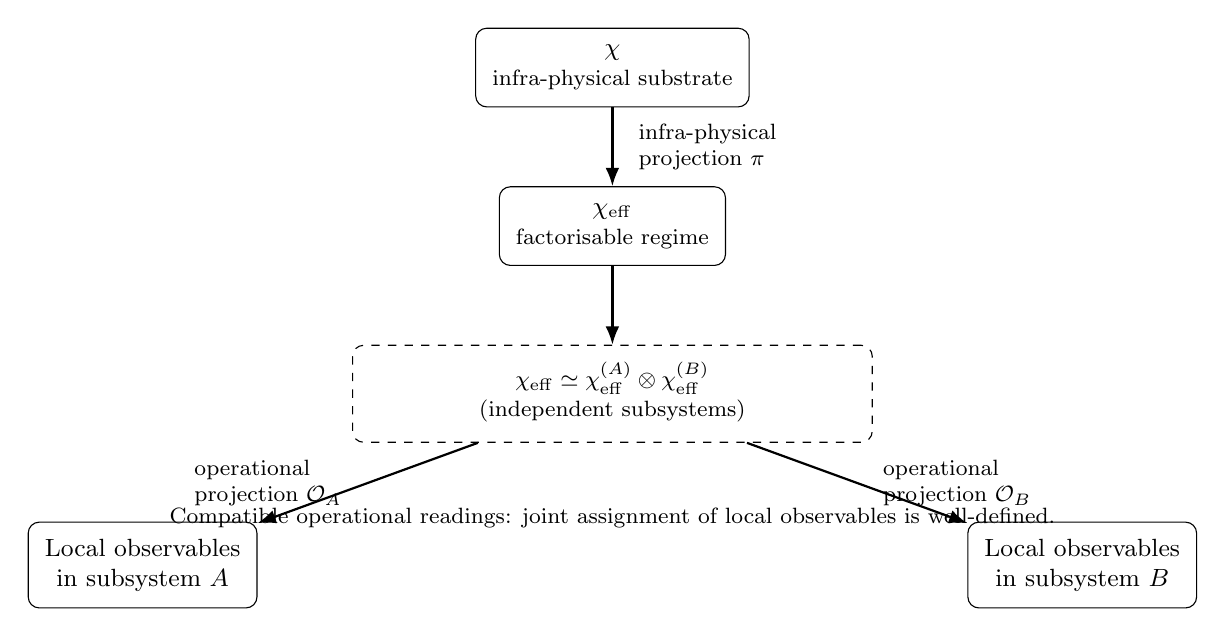
\begin{tikzpicture}[
      font=\small,
      node distance=10mm,
      box/.style={draw, rounded corners, align=center, inner sep=6pt},
      arrow/.style={-Latex, thick},
      note/.style={align=left, font=\footnotesize},
      dashedbox/.style={draw, dashed, rounded corners, inner sep=6pt}
    ]

    \node[box] (chi) {$\chi$\\\footnotesize infra-physical substrate};

    \node[box, below=of chi] (chieff) {$\chi_{\mathrm{eff}}$\\\footnotesize factorisable regime};

    \node[dashedbox, below=of chieff, minimum width=6.6cm] (decomp) {
      \begin{tabular}{c}
        \footnotesize $\chi_{\mathrm{eff}} \simeq \chi_{\mathrm{eff}}^{(A)} \otimes \chi_{\mathrm{eff}}^{(B)}$\\
        \footnotesize (independent subsystems)
      \end{tabular}
    };

    \node[box, below left=10mm and 12mm of decomp] (obsA) {Local observables\\in subsystem $A$};
    \node[box, below right=10mm and 12mm of decomp] (obsB) {Local observables\\in subsystem $B$};

    \draw[arrow] (chi) -- node[right=2mm, note] {infra-physical\\projection $\pi$} (chieff);
    \draw[arrow] (chieff) -- (decomp);

    \draw[arrow] (decomp) -- node[left=2mm, note] {operational\\projection $\mathcal{O}_A$} (obsA);
    \draw[arrow] (decomp) -- node[right=2mm, note] {operational\\projection $\mathcal{O}_B$} (obsB);

    \node[note, below=7mm of decomp, align=center] (compat)
    {\footnotesize Compatible operational readings: joint assignment of local observables is well-defined.};

    \end{tikzpicture}
    \caption{Classical (factorisable) regime.
    After the infra-physical projection $\pi$, the effective description
      $\chi_{\mathrm{eff}}$ admits an approximate decomposition into independent subsystems.
      Operational projections $\mathcal{O}_A$ and $\mathcal{O}_B$ then yield compatible local
      observables, recovering standard classical and relativistic descriptions.
      This figure illustrates the hierarchy between infra-physical projection and
      operational observation, and contrasts with the non-factorisable regimes discussed
      in later sections.}
    \label{fig:classical-factorisable}
  \end{figure}

  Because the projection from $\chi$ to $\chi_{\mathrm{eff}}$ is generically
  non-injective, the effective observables obtained in this way summarize relational
  structure without exhausting the underlying degrees of freedom.
  Distinct $\chi$ configurations may therefore correspond to identical effective
  descriptions, while a single underlying configuration may admit multiple correlated
  operational realizations.
  This structural asymmetry is central to the emergence of both classical and quantum
  phenomenology, and is developed in detail in subsequent sections.

  Within this interpretation, temporal ordering, relational separation, and large-scale
  behavior are not treated as independent postulates, but as complementary effective
  summaries of the same underlying relaxation dynamics, appearing at different levels
  of coarse-graining.
  Their precise operational and dynamical roles are introduced progressively in the
  following sections.

  The physical content of the theory thus resides entirely in the dynamics of the
  fundamental $\chi$ substrate, while spacetime notions function as emergent,
  context-dependent descriptive tools rather than as fundamental ingredients.

  \subsection{Relational Projection and Spectral Admissibility}
  \label{sec:relational_projection}

  In Cosmochrony, admissible physical descriptions are not defined by spacetime
  locality or geometric structure, but by the spectral properties of the relational
  substrate $\chi$.

  \paragraph{Relational operator.}
    Let $\mathcal{H}_\chi$ denote the configuration space of admissible $\chi$ states.
    We introduce a relational operator
    \begin{equation}
      L_\chi : \mathcal{H}_\chi \rightarrow \mathcal{H}_\chi,
    \end{equation}
    defined purely in terms of $\chi$ correlations.
    In discrete implementations (Appendix~D), $L_\chi$ reduces to a graph Laplacian
    associated with relational adjacency; in the continuum limit, it defines an
    effective self-adjoint operator encoding relational connectivity.

  \paragraph{Spectral decomposition.}
    The operator $L_\chi$ admits a spectral decomposition
    \begin{equation}
      L_\chi \psi_n = \lambda_n \psi_n,
    \end{equation}
    where $\{\lambda_n\}$ are non-negative eigenvalues and $\{\psi_n\}$ the associated
    eigenmodes.
    No geometric or spacetime interpretation is assumed at this stage.

  \paragraph{Admissibility as spectral filtering.}
    Projectable configurations are selected by a spectral filter acting on $L_\chi$.
    We define the infra-physical admissibility projection as
    \begin{equation}
      \Pi_{\lambda_*} \;\equiv\; f\!\left(\frac{L_\chi}{\lambda_*}\right),
    \end{equation}
    where $f(x)$ is a fixed, smooth cutoff function satisfying
    $f(x)\to 0$ for $x\ll 1$ and $f(x)\to 1$ for $x\gg 1$.
    The scale $\lambda_*$ sets the characteristic spectral threshold separating
    admissible from non-admissible relational modes.

    This construction defines admissibility without reference to spacetime,
    coordinates, or integration measures, relying solely on spectral properties
    of the relational operator.

  \subsection{Monotonicity and Arrow of Time}
  \label{subsec:monotonicity-and-arrow-of-time}

  A central structural postulate of Cosmochrony is that the relational substrate $\chi$
  admits an intrinsic, globally ordered relaxation structure.
  In effective descriptions, this ordering manifests as the monotonic behavior of the
  projected scalar descriptor $\chi_{\mathrm{eff}}$ along admissible ordering paths:
  \begin{equation}
    \mathcal{D}_{\lambda} \chi_{\mathrm{eff}} \ge 0 .
  \end{equation}
  Here $\lambda$ denotes an ordering parameter associated with the relaxation of
  projected $\chi$ configurations, rather than a fundamental time coordinate.
  The inequality expresses a structural constraint on admissible projected
  representations, not an evolution equation for a fundamental scalar quantity.

  This monotonicity reflects an intrinsic asymmetry in the ordering structure of $\chi$
  configurations.
  Because the projection from $\chi$ to $\chi_{\mathrm{eff}}$ is generically
  non-injective, admissible effective descriptions may lose information about
  underlying configurations, but cannot exhibit reversals of the ordering induced by
  relaxation.

  Within this framework, energy is interpreted as an effective measure of the
  remaining capacity of projected $\chi$ configurations to undergo further
  relaxation.
  As relaxation proceeds, this capacity is irreversibly expended in the projected
  description.
  Admissible ordering paths therefore exclude any effective decrease of
  $\chi_{\mathrm{eff}}$, which would correspond to a restoration of relaxation capacity
  incompatible with the underlying ordering structure.

  Irreversibility follows directly from this structural constraint.
  The arrow of time is identified with the directional ordering induced by relaxation:
  the progression from configurations with greater effective relaxation capacity
  toward configurations in which that capacity has been locally or globally exhausted.

  This temporal orientation is not derived from coarse-graining, entropy production,
  or special initial conditions.
  It arises prior to any statistical or thermodynamic description, as a direct
  consequence of the ordering constraints imposed by $\chi$ on its admissible
  projections.
  The relation to thermodynamic irreversibility is discussed further in
  Section~\ref{subsec:entropy-arrow}.

  \subsection{Local Relaxation Speed}
  \label{subsec:local-relaxation-speed}

  A fundamental structural constraint of the Cosmochrony framework is that the effective
  local ordering rate associated with projected $\chi$ configurations is bounded.
  In effective geometric descriptions, this constraint takes the form
  \begin{equation}
    \left| \mathcal{D}_{\mathrm{loc}} \chi_{\mathrm{eff}} \right| \le c ,
  \end{equation}
  where $\mathcal{D}_{\mathrm{loc}} \chi_{\mathrm{eff}}$ denotes an effective local
  relaxation functional characterizing the maximal admissible ordering of projected
  $\chi$ configurations.
  The constant $c$ is the effective causal bound observed in spacetime.

  This inequality expresses a constraint on admissible projected descriptions, not a
  propagation speed defined at the level of the $\chi$ substrate.
  It limits the maximal rate at which effective causal connectivity and local geometric
  relations can be established within descriptions compatible with the intrinsic
  ordering structure of $\chi$.
  The quantity $c$ therefore characterizes the causal structure of the projected regime
  rather than the dynamics of the pre-geometric substrate itself.

  Local particle propagation, signal transmission, and field interactions are all
  constrained by this bound in effective spacetime descriptions.
  By contrast, the underlying $\chi$ substrate is not subject to spacetime notions of
  velocity or signal propagation.

  Apparent superluminal recession velocities at cosmological scales arise from cumulative
  and global effects of projected $\chi$ ordering and do not violate this local causal
  constraint.
  Local causal relations remain bounded by $c$ in all admissible effective descriptions.

  \subsection{Relation to Conventional Fields}
  \label{subsec:relation-to-conventional-fields}

  Effective descriptions derived from projected $\chi$ configurations may formally
  resemble scalar or tensor fields used in cosmology and particle physics.
  This resemblance, however, reflects the emergence of a spacetime-based descriptive
  language, not the presence of an additional fundamental field.
  The $\chi$ substrate itself remains a pre-geometric relational structure, independent
  of spacetime and field-theoretic notions.

  Within Cosmochrony, energy and quantization are not fundamental attributes of $\chi$.
  They arise only at the effective level, as consequences of the non-injective
  projection from $\chi$ to admissible observables.
  Only certain stable, localized, and spectrally isolated configurations admit a
  particle-like interpretation and can be consistently described using conventional
  quantum field-theoretic tools in regimes where a spacetime description is valid.

  Matter, radiation, and interactions are therefore not associated with independent
  fundamental fields coupled to $\chi$.
  They correspond instead to effective degrees of freedom arising from structural
  constraints, spectral organization, and long-lived relational patterns of projected
  $\chi$ configurations.
  Standard Model fields are recovered as accurate effective descriptions within the
  appropriate coarse-grained regimes.

  From this perspective, Cosmochrony does not extend the Standard Model by introducing
  new fundamental fields.
  Rather, it provides an ontological explanation for the emergence, applicability, and
  structural properties of effective field descriptions themselves.

  \subsection{Initial Conditions and Global Structure}
  \label{subsec:initial-conditions-and-global-structure}

  The Cosmochrony framework does not postulate initial conditions in the conventional
  temporal sense.
  Instead, it assumes that the relational substrate $\chi$ admits a minimal admissible
  ordering state, denoted $\chi_0$, which defines a structural boundary of admissible
  projected descriptions.
  This state does not correspond to a distinguished moment in time, but to the earliest
  configurations for which an effective ordering interpretation becomes meaningful.

  In effective geometric regimes, the characteristic scale associated with projected
  descriptions in the vicinity of $\chi_0$ coincides numerically with the Planck scale.
  This correspondence reflects the breakdown of projectability and of coarse-grained
  spacetime descriptions below this regime, rather than the presence of a fundamental
  cutoff, microscopic discreteness, or underlying spacetime lattice.

  From this perspective, cosmic history is interpreted as the progressive and
  irreversible ordering of projected $\chi$ configurations away from this minimal
  admissible boundary.
  No spacetime singularity is required at the fundamental level.
  Apparent singular behavior arises only when classical notions of time, distance, or
  curvature are extrapolated beyond the regime in which projected $\chi$ configurations
  admit a stable geometric and causal interpretation.

  \paragraph{Ontological poverty and the growth of admissible structure.}
    The minimal admissible state $\chi_0$ corresponds to a regime of \emph{ontological
poverty}, as defined in Section~\ref{sec:definition-and-fundamental-properties-of-the-chi-field}.
    Only a severely restricted class of simple and highly coherent configurations can be
    projected in this regime.
    As relaxation proceeds, the space of admissible configurations expands, enabling the
    emergence of increasingly rich, localized, and hierarchical effective structures.
    This growth reflects an expansion of descriptive and relational capacity, rather than
    the unfolding of pre-encoded complexity.

    The global structure of admissible projected descriptions is therefore constrained by
    the ordering properties of the underlying $\chi$ substrate, rather than by arbitrarily
    specified initial data or boundary conditions.
    In the following section, we derive a minimal effective dynamical equation governing
    the ordering of projected $\chi$ configurations and explore its immediate physical
    consequences.


  \section{Ontological Interpretation of the $\chi$ Field}
  \label{sec:chi_ontology}

  Throughout this section, we explicitly distinguish the invariant structural bound $c_{\chi}$,
  defined at the level of the pre-temporal $\chi$ substrate, from its emergent spacetime manifestation $c$.
  The latter appears only once spacetime notions such as distance, duration, and causal propagation become meaningful.

  \subsection{The $\chi$ Field as a Pre-Temporal Structural Plan}

    In the Cosmochrony framework, the $\chi$
    field is not interpreted as a physical field evolving within spacetime, but as a pre-temporal structural
    substrate from which spacetime, matter, and physical laws emerge.
    It may be heuristically described as a ``plan'' of the universe: a complete structure encoding the set of
    physically admissible configurations and their relations.

    Importantly, this plan is not a predetermined scenario.
    It does not specify a unique history nor a fixed sequence of events.
    Rather, it defines a constrained space of possibilities within which relational ordering may arise.
    Temporal succession is therefore not fundamental but emergent, corresponding to an oriented resolution of
    structural relations within $\chi$.

  \subsection{Intrinsic Indeterminacy and Fluctuations}
    \label{subsec:intrinsic-indeterminacy-and-fluctuations}

    A perfectly deterministic and fully symmetric structural plan would remain dynamically sterile: no configuration
    would be privileged, and no physically consequential ordering could emerge.
    For this reason, Cosmochrony postulates the existence of intrinsic indeterminacy within the $\chi$ structure.

    These fluctuations are not temporal events, nor stochastic processes unfolding in time.
    They represent a fundamental absence of complete determination at the structural level.
    Their role is not to generate dynamics, but to break perfect structural indifference, thereby allowing certain
    transitions to become physically consequential.

    In this sense, fluctuations constitute a condition of possibility for emergence, rather than a dynamical cause.

  \subsection{Energy as Capacity for Relaxation}

    Within this framework, energy is reinterpreted as the capacity of the $\chi$ structure to relax its constraints.
    Energy does not correspond to a substance or a conserved entity at the fundamental level, but to a measure of
    unresolved structural tension.

    The deployment of $\chi$
    corresponds to the progressive conversion of structural indeterminacy into relational information.
    Energy thus quantifies the potential for this conversion.
    Without intrinsic indeterminacy, energy would be undefined, as no relaxation could occur.

  \subsection{Mass as Frozen Information}

    Localized, stable configurations of the $\chi$
    field—interpreted as particle-like excitations—correspond to regions where relaxation is strongly inhibited.
    These configurations trap a fixed amount of unresolved structural information.

    In this interpretation, mass represents frozen energy: information that has lost its capacity to participate
    freely in further relaxation.
    At the level of emergent spacetime physics, this relation is expressed by the standard mass--energy equivalence,
    \[
      E_{\text{phys}} = m_{\text{phys}} c^2,
    \]
    where $c$ denotes the emergent spacetime limiting speed.
    This identity reflects, at the phenomenological level, a more fundamental structural relation
    governing the confinement and release of information within the $\chi$ substrate.

  \subsection{The Role of the Universal Bound $c_{\chi}$}

    The constant $c_{\chi}$ plays a central structural role in Cosmochrony.
    Rather than setting a signal propagation speed, it defines an absolute bound on the degree to which
    information can be structurally constrained within the $\chi$ substrate.

    In this sense, $c_{\chi}$
    sets the maximal ``knotting'' or confinement of structural information compatible with physical coherence.
    Beyond this bound, further constraint becomes impossible and relaxation is unavoidable.
    The emergent spacetime notions of inertial resistance, causal structure, and mass--energy equivalence
    are understood as projections of this invariant structural limit.

  \subsection{The Role of $\hbar_{\chi}$ and Reprojection from $\chi$}

    In Cosmochrony, the parameter \(\hbar_{\chi}\) is \textbf{not derived from \(\hbar\)}
    but emerges from the fundamental scales \(K_0\), \(\chi_c\), and \(c\).
    Its numerical coincidence with \(\hbar\) in quantum regimes reflects the
        \textbf{universality of action quantization} across physical theories.\footnote{
  Unlike in quantum gravity, where \(\hbar\) and \(G\) are fundamental, here \(\hbar_{\chi}\) is derived from \(\chi\)
  -field parameters alone. The standard \(\hbar\) is recovered only in regimes where
  \(\ell_{\text{spacetime}} \sim \chi_c\).
}
    It is derived purely from the fundamental scales $K_0$, $\chi_c$, and $c$,
    without reference to spacetime or quantum constants.
    It does not represent a quantum of action evolving in time, but a fundamental
    quantum of reprojection.

    Intrinsic fluctuations of $\chi$ do not give rise to continuous emergence.
    Rather, any reprojection of structural information into emergent spacetime
    occurs in discrete units set by $\hbar_{\chi}$.
    Transient excitations commonly interpreted as vacuum particles thus correspond
    to minimal reprojections allowed by this bound.

    In the early universe, where spacetime structure was weakly stabilized,
    such reprojections were diffuse and frequent.
    As the universe relaxed and large-scale structures formed, reprojection became
    progressively localized, manifesting as vacuum fluctuations in otherwise stable
    regions of spacetime.

  \section{Dynamical Equation for the $\chi$ Field}
  \label{sec:dynamical-equation-for-the-chi-field}

  \subsection{Parameter-Independent Relaxation}
  \label{subsec:parameter-independent-relaxation}

  To avoid the conceptual pitfalls associated with a fundamental time coordinate,
  the dynamics of the scalar quantity $\chi$ is formulated without reference to any
  external temporal parameter.
  Instead, physical evolution is described as an ordered sequence of $\chi$
  configurations, denoted $(\chi_\lambda)$, where $\lambda$ is a strictly monotonic
  ordering parameter labeling the relaxation process.

  At the fundamental level, the dynamics of $\chi$ is defined by an intrinsic
  relaxation flow:
  \begin{equation}
    \mathcal{D}_{\lambda}\chi = \mathcal{R}[\chi],
  \end{equation}
  where $\mathcal{R}[\chi]$ denotes the local rate of relaxation toward equilibrium,
  defined purely in terms of the relational structure of $\chi$ configurations.
  No spacetime derivative or geometric operator is assumed at this stage.

  Quantities commonly interpreted as temporal derivatives arise only at the level of
  effective descriptions, when $\chi$ configurations admit a quasi-stable geometric
  interpretation.
  In such regimes, a coordinate time parameter may be introduced as a convenient
  label of the relaxation ordering, but it carries no fundamental significance and
  does not affect the underlying dynamics.

  Within this framework, relaxation does not occur \emph{in} time.
  Rather, the cumulative relaxation of $\chi$ defines what is operationally
  identified as physical duration.
  Local variations in the relaxation rate provide the effective measure of temporal
  flow, establishing a direct connection between the structure of $\chi$
  configurations and the emergent notion of time.

  \subsection{Hamiltonian Derivation of the Evolution Equation}
  \label{subsec:hamiltonian-derivation}

  While the dynamics of $\chi$ can be viewed as a minimal relaxation principle, it can be more rigorously derived from a
  Hamiltonian constraint.
  We postulate that the dynamics of $\chi$ are governed by a Dirac-type kinematic constraint in phase space, analogous
  to the mass-shell condition for a massless relativistic particle:
  \begin{equation}
  (\partial_t \chi)
    ^2 + |\nabla \chi|^2 = c^2,
    \label{eq:hamiltonian_constraint}
  \end{equation}
  where $c$ is the fundamental velocity scale.
  Combined with the \textit{arrow of time} postulate ($\partial_t \chi \geq 0$), which reflects the irreversible
  relaxation of the Cosmochron, this leads uniquely to the first-order evolution equation:
  \begin{equation}
    \partial_t \chi = c \sqrt{1 - \frac{|\nabla \chi|^2}{c^2}}.
    \label{eq:chi_dynamics}
  \end{equation}

  This derivation grounds the ``minimal principle'' in the symplectic structure of the field's phase space, ensuring
  that $\chi$ acts as an intrinsic time coordinate.

  The mathematical stability of this equation is demonstrated in~\ref{subsec:stability_chi}, while explicit analytical
  solutions are derived in~\ref{subsec:analytical_solutions_chi}.
  The coupling of the $\chi$ field with matter, extending this kinematic backbone to a dynamical theory, is further
  discussed in~\ref{subsec:coupling_matter_chi} and Section~\ref{subsec:variational-formulation}.

  \subsection{Microscopic Origin of the Coupling Tensor and the Poisson Equation}
  \label{subsec:microscopic-origin-of-the-coupling-tensor-and-the-poisson-equation}

  For internal consistency, the effective coupling governing the ordering of projected
  $\chi$ configurations cannot be treated as a fixed universal constant.
  Instead, it must depend on the internal structural state of the projected description,
  reflecting how localized configurations either facilitate or resist further relaxation.
  In Cosmochrony, this dependence is captured through a constitutive relation linking
  effective coupling strength to variations of the effective scalar descriptor
  $\chi_{\mathrm{eff}}$, without invoking any underlying spatial substrate or fundamental
  interaction at the pre-geometric level.

  A convenient phenomenological parametrization of this dependence is given by
  \begin{equation}
    K_{\mathrm{eff}}
    = K_0 \exp\!\left(
                  -\frac{(\Delta \chi_{\mathrm{eff}})^2}{\chi_c^2}
    \right),
    \label{eq:effective_coupling_tensor}
  \end{equation}
  where $\Delta \chi_{\mathrm{eff}}$ denotes a measure of effective internal variation
  between correlated projected configurations,
  $K_0$ characterizes the maximal relaxation conductivity in a homogeneous effective
  background, and $\chi_c$ sets the characteristic scale beyond which structural
  inhomogeneities significantly suppress relaxation efficiency.
  This expression should be understood as a constitutive relation for admissible projected
  descriptions, not as a fundamental law governing the $\chi$ substrate.

  Projected configurations exhibiting strong internal variation—such as stable solitonic
  or bound structures—therefore reduce the effective coupling and locally slow the
  admissible relaxation ordering.
  This reduction does not correspond to the introduction of a new interaction.
  It reflects instead the intrinsic resistance of structured projected configurations to
  further relaxation.
  The resulting slowdown provides the microscopic origin of the emergent gravitational
  phenomenology discussed in the preceding sections.

  In regimes where a spacetime description becomes applicable, the local effective
  relaxation rate $\mathcal{D}_{\mathrm{loc}} \chi_{\mathrm{eff}}$ differs from its
  asymptotic value $\mathcal{D}_0$ far from localized structures.
  An effective gravitational potential $\Phi$ may then be introduced as a descriptive
  parameter through the relation
  \begin{equation}
    \frac{\mathcal{D}_{\mathrm{loc}} \chi_{\mathrm{eff}}}{\mathcal{D}_0}
    \simeq 1 + \frac{\Phi}{c^2},
    \label{eq:relaxation_potential_relation}
  \end{equation}
  which summarizes the relative slowdown of effective relaxation ordering in a form
  familiar from classical gravitational phenomenology.
  The potential $\Phi$ has no independent ontological status and serves only as a compact
  parametrization of relaxation inhomogeneities.

  In the weak-structure regime, where effective internal variations remain small compared
  to $\chi_c$, the spatial distribution of $\Phi$ admits a simplified elliptic
  description.
  At this coarse-grained level, the effective dynamics reduce to a Poisson-type relation,
  \begin{equation}
    \nabla^2 \Phi \simeq 4\pi G_{\mathrm{eff}} \rho,
    \label{eq:effective_poisson_equation}
  \end{equation}
  where $\rho$ denotes the effective density of localized, relaxation-resistant projected
  configurations and $G_{\mathrm{eff}}$ is an emergent coupling parameter encoding the
  collective response of the relaxation ordering to such structures.
  Both quantities are defined strictly within the effective geometric description.

  This Poisson equation is not fundamental.
  It represents the weak-field, macroscopic limit of the constrained ordering of
  projected $\chi$ configurations, expressed in a form adapted to effective spacetime
  description.
  Gravitation therefore appears not as an independent interaction, but as a descriptive
  manifestation of reduced relaxation conductivity induced by structured projected
  configurations.

  A fully relational formulation, consistent with but not required for the effective
  description adopted here, is provided in
  Appendix~\ref{app:relational_formulation}.

  \paragraph{Status of effective equations.}
    The effective equations introduced in this subsection—

  \subsection{Variational Formulation and Born--Infeld Action}
  \label{subsec:variational-formulation}

  In regimes where projected $\chi$ configurations admit a stable geometric
  interpretation, the effective relaxation constraints introduced above may be
  summarized in a compact variational form.
  This formulation is not fundamental and does not define a dynamics of the
  pre-geometric $\chi$ substrate.
  Rather, it provides an auxiliary and regularized representation of admissible
  projected descriptions in the presence of localized relaxation-resistant
  configurations.

  Motivated by Born--Infeld--type non-linear actions, originally introduced to control
  field singularities and enforce upper bounds on physical gradients~\cite{BornInfeld1934,DeserGibbons1998}, we
  consider the effective Lagrangian density
  \begin{equation}
    \mathcal{L}_{\mathrm{eff}}
    = -c^2 \sqrt{1 - \frac{|\nabla \chi_{\mathrm{eff}}|^2}{c^2}}
    + \mathcal{D}_{\mathrm{loc}}\chi_{\mathrm{eff}}
    - \frac{4\pi G_{\mathrm{eff}}}{c^2}\,\rho\,\chi_{\mathrm{eff}} ,
    \label{eq:leff_equation}
  \end{equation}
  where $\chi_{\mathrm{eff}}$ denotes the effective scalar descriptor introduced in
  Sec.~\ref{subsec:geometric-action},
  $\mathcal{D}_{\mathrm{loc}}\chi_{\mathrm{eff}}$ is the effective local relaxation
  ordering defined in Sec.~\ref{subsec:parameter-independent-relaxation}, and $\rho$
  represents the effective density of localized, relaxation-resistant projected
  configurations.
  All quantities appearing in this expression are defined strictly within the effective
  geometric description.

  The linear dependence on $\mathcal{D}_{\mathrm{loc}}\chi_{\mathrm{eff}}$ enforces the
  monotonicity of admissible projected descriptions without introducing additional
  propagating degrees of freedom.
  The square-root structure acts as a non-linear regulator, ensuring that effective
  spatial variations remain bounded by the universal constraint $c$.
  This role is directly analogous to that of Born--Infeld electrodynamics, where the
  action enforces a maximal field strength without postulating new microscopic
  dynamics.

  Within this auxiliary variational framework, the Euler--Lagrange equation associated
  with $\chi_{\mathrm{eff}}$ reproduces the non-linear elliptic relation governing the
  spatial distribution of relaxation slowdown:
  \begin{equation}
    \nabla \cdot
    \left(
      \frac{\nabla \chi_{\mathrm{eff}}}
      {\sqrt{1 - |\nabla \chi_{\mathrm{eff}}|^2 / c^2}}
    \right)
    = \frac{4\pi G_{\mathrm{eff}}}{c^2}\,\rho ,
    \label{eq:nonlinear_poisson}
  \end{equation}
  which coincides with the effective Poisson-type relation obtained in
  Sec.~\ref{subsec:microscopic-origin-of-the-coupling-tensor-and-the-poisson-equation}.
  No new physical content is introduced at this stage; the variational formulation
  merely provides a compact and internally consistent encoding of the previously
  established constraints.

  This Born--Infeld--like action should therefore be understood strictly as an
  \emph{auxiliary variational representation}.
  It does not constitute a fundamental action principle, nor does it define equations
  of motion for the $\chi$ substrate.
  Its purpose is to regularize the effective description, enforce universal structural
  bounds, and facilitate comparison with standard gravitational phenomenology in the
  appropriate weak-field regime.

  The physical interpretation of this effective action is discussed in
  Appendix~\ref{subsec:hydrodynamic-limit}, while its mathematical consistency with the
  underlying relational dynamics and discrete formulation is established in
  Appendix~\ref{sec:born-lagrangian_derivation}.

\subsection{Why This Is Not a Scalar--Tensor Theory}
  \label{subsec:not-scalar-tensor}

  The effective variational formulation introduced in the previous subsection may
  superficially resemble scalar--tensor or modified gravity theories, in which a
  scalar field couples to geometry or mediates gravitational interactions.
  It is therefore essential to clarify that Cosmochrony does \emph{not} belong to this
  class of frameworks, either conceptually or technically.

  First, the effective scalar descriptor $\chi_{\mathrm{eff}}$ is \emph{not} a
  fundamental dynamical field.
  It does not represent an independent physical degree of freedom propagating on
  spacetime, nor does it possess intrinsic values or conjugate momenta.
  By construction, $\chi_{\mathrm{eff}}$ is a projected, coarse-grained descriptor of
  relational features of the pre-geometric substrate $\chi$, defined only in regimes
  where a spacetime interpretation becomes applicable.
  There is therefore no scalar field at the fundamental level whose dynamics could be
  coupled to geometry.

  Second, no modification of the gravitational sector is postulated.
  The metric appearing in effective descriptions is not an independent dynamical field,
  nor is it sourced or altered by a scalar field equation.
  Instead, geometric quantities summarize correlations between projected
  $\chi_{\mathrm{eff}}$ configurations.
  The Born--Infeld--like variational form introduced earlier does not define a new
  gravitational theory; it merely encodes, in a compact and regularized manner, the
  constraints governing admissible projected descriptions.
  In particular, there is no scalar--tensor coupling term of the form
  $f(\chi_{\mathrm{eff}}) R$, nor any modification of the Einstein--Hilbert action.

  Third, the effective equations derived from the auxiliary variational formulation do
  not introduce additional propagating modes.
  In scalar--tensor theories, the scalar field typically carries its own dynamics,
  leading to extra degrees of freedom, modified wave propagation, or additional
  polarization states.
  In Cosmochrony, by contrast, $\chi_{\mathrm{eff}}$ does not propagate independently.
  All effective equations constrain admissible relaxation patterns of projected
  configurations and do not enlarge the physical phase space.

  Finally, the origin of gravitational phenomenology in Cosmochrony is fundamentally
  different.
  Gravitation does not arise from the exchange of a scalar mediator or from a dynamical
  coupling between scalar and tensor sectors.
  It emerges instead from the local inhibition of relaxation ordering induced by
  structured projected configurations.
  The appearance of Poisson-like equations or gravitational potentials reflects the
  weak-structure limit of this constrained ordering, not the presence of a scalar
  gravitational field.

  In summary, Cosmochrony should not be interpreted as a scalar--tensor or modified
  gravity theory.
  The effective scalar descriptor $\chi_{\mathrm{eff}}$ is neither fundamental nor
  dynamical, the variational formulation is auxiliary rather than postulatory, and no
  additional gravitational degrees of freedom are introduced.
  The framework therefore avoids the conceptual and phenomenological issues commonly
  associated with scalar--tensor theories, while reproducing standard gravitational
  behavior in the appropriate effective regimes.

  \subsection{Causality and Locality}
  \label{subsec:causality-and-locality}

  Equation~\eqref{eq:chi_dynamics} does not define a fundamental dynamics of the
  $\chi$ substrate.
  Rather, it constrains admissible projected descriptions in regimes where a
  geometric interpretation becomes applicable.
  Within such effective descriptions, the relaxation ordering encoded by
  $\chi_{\mathrm{eff}}$ exhibits locality and causality in the operational sense
  relevant to physical observables.

  Effective locality follows from the fact that variations of
  $\chi_{\mathrm{eff}}$ at a given effective spacetime event depend only on
  correlated neighboring projected configurations, as defined within the emergent
  geometric description.
  No instantaneous coupling, action at a distance, or nonlocal influence is
  introduced at the level of effective physical observables.
  All admissible projected descriptions therefore respect locality in the sense
  appropriate to an emergent spacetime framework.

  Causality is enforced through the existence of a universal bound on the effective
  local relaxation ordering,
  \[
    \left| \mathcal{D}_{\mathrm{loc}} \chi_{\mathrm{eff}} \right| \le c ,
  \]
  which constrains the maximal rate at which correlations between effective
  configurations may be established.
  This bound functions as an effective causal constraint without presupposing a
  fundamental spacetime structure, lightcones, or signal propagation at the level
  of the $\chi$ substrate.

  Within effective physical descriptions, no superluminal propagation of signals
  or causal influence occurs.
  Apparent superluminal recession velocities observed in cosmological contexts
  arise solely from the cumulative integration of locally constrained relaxation
  ordering over extended regions.
  They therefore remain fully consistent with effective locality and causality as
  defined within the Cosmochrony framework.

  \medskip
  \noindent\emph{Conceptual remark.}—
  The effective causal bound $c$ introduced here should not be interpreted as an
  independent physical postulate.
  As established in Section~\ref{subsec:role-of-cchi}, it corresponds to the
  projected manifestation of the invariant structural bound $c_\chi$ defined at
  the level of the pre-temporal $\chi$ substrate.
  In regimes admitting a locally injective projection and a stable geometric
  interpretation, $c_\chi$ acquires an operational meaning as a maximal admissible
  local ordering rate, which appears in spacetime descriptions as the effective
  causal constraint $c$.

  Effective causality in Cosmochrony thus arises as a derived property of bounded
  projective realizations, rather than as a fundamental principle imposed on
  spacetime itself.

  \subsection{Homogeneous Cosmological Limit}
  \label{subsec:homogeneous-cosmological-limit}

  In a homogeneous and isotropic regime, projected $\chi$ configurations exhibit no
  effective spatial variations.
  The admissible relaxation ordering is then uniform across the emergent description,
  and the effective local relaxation rate attains its maximal allowed value,
  \begin{equation}
    \mathcal{D}_{\mathrm{loc}}\chi_{\mathrm{eff}} = c ,
  \end{equation}
  where $c$ denotes the universal bound constraining effective relaxation ordering.

  When expressed in terms of an effective cosmological time parameter $t$, introduced
  solely as a convenient label of the relaxation ordering, this uniform regime may be
  represented by the linear relation
  \begin{equation}
    \chi_{\mathrm{eff}}(t) = \chi_{\mathrm{eff},0} + c\, t ,
  \end{equation}
  where $\chi_{\mathrm{eff},0}$ denotes a reference value fixing the origin of the
  effective description.
  This parametrization does not introduce a fundamental time variable, nor does it
  assign intrinsic values to the $\chi$ substrate.
  It serves only as a compact representation of cumulative relaxation ordering in a
  homogeneous cosmological regime.

  Interpreting effective spatial distances as accumulated relational differentiation
  between projected configurations, this uniform ordering directly leads to a
  Hubble-like expansion law, as discussed in Sec.~\ref{sec:cosmology}.
  Cosmic expansion thus reflects the global ordering of projected $\chi$
  configurations, rather than the presence of an external energy component or a
  fundamental expansion of spacetime itself.

  As shown in Appendix~\ref{subsec:minimal-kinematic-constraint}, the requirement that
  effective relaxation ordering remain monotonic in an expanding regime implies the
  existence of a minimal residual structural inhomogeneity in projected $\chi$
  configurations.
  In effective geometric terms, this manifests as a non-vanishing lower bound on
  gravitational acceleration, providing a natural explanation for MOND-like
  phenomenology without invoking dark matter particles~\cite{FamaeyMcGaugh2012}.

  \subsection{Influence of Local Structure}
  \label{subsec:influence-of-local-structure}

  In regions where projected $\chi$ configurations exhibit non-vanishing effective
  structural variations, the admissible local relaxation ordering is reduced.
  This slowdown plays a central role in the emergence of gravitational phenomena
  within the Cosmochrony framework.

  Localized relaxation-resistant configurations—describable in effective regimes as
  particle-like solitonic structures—act as constraints on the admissible ordering of
  projected $\chi$ configurations.
  By increasing the effective structural complexity of the projected description,
  they reduce the local effective relaxation rate without introducing any additional
  interaction or force.

  When a geometric description becomes applicable, this mechanism manifests
  phenomenologically as gravitational time dilation and spatial curvature.
  No independent gravitational field is postulated.
  Gravitation emerges instead as a collective consequence of locally constrained
  effective relaxation ordering, reflecting the presence of structured projected
  configurations.

  \subsection{Unified Origin of Geometric and Field Effects}
  \label{subsec:unified-origin}

  The relationship between the $\chi$ substrate and the effective spacetime metric
  $g_{\mu\nu}$ is strictly hierarchical, reflecting the transition from a fundamental
  pre-geometric relational structure to smooth geometric descriptions applicable at
  macroscopic scales.

  \begin{enumerate}
    \item \textbf{Primacy of the $\chi$ substrate:}
    At the fundamental level, physical reality is described solely in terms of the
    $\chi$ substrate and its intrinsic relational structure.
    The $\chi$ substrate is not defined on spacetime, does not possess numerical
    values, and is not governed by a dynamical field equation.
    Ordering, relaxation, and causal notions arise only at the level of admissible
    projected descriptions.

    \item \textbf{Emergent Geometry:}
    In regimes where projected $\chi$ configurations admit a stable, slowly varying
    description, geometric notions become meaningful.
    The spacetime metric $g_{\mu\nu}$ arises as an effective descriptor summarizing the
    correlations and relaxation ordering of projected $\chi$ configurations.
    It provides a coarse-grained geometric language suitable for macroscopic
    observers, without acquiring independent ontological status.

    \item \textbf{Unified Interpretation of Fields and Gravitation:}
    Within this effective geometric description, localized relaxation-resistant
    projected configurations—describable as solitonic structures—are identified with
    matter degrees of freedom.
    Gravitational phenomena correspond to the local modulation of effective relaxation
    ordering induced by such structures.
    The metric does not act as an independent dynamical agent, but encodes the
    collective geometric response associated with constrained projected descriptions.
  \end{enumerate}

  In this framework, no independent gravitational interaction or fundamental field is
  postulated.
  Matter, geometry, and gravitational phenomena emerge as complementary aspects of the
  same constrained ordering of projected $\chi$ configurations, ensuring a unified and
  internally consistent description across scales.

  \subsection{Limitations and Scope}
  \label{subsec:limitations-and-scope}

  Equation~\eqref{eq:chi_dynamics} is intentionally minimal.
  It does not aim to provide a complete description of quantum fluctuations of
  $\chi$, nor does it incorporate higher-order backreaction effects.
  Its role is to capture the essential kinematic constraint governing the
  relaxation of $\chi$ in regimes where an effective geometric interpretation
  applies.

  Within this scope, the equation provides a unified backbone from which
  gravitational, quantum, and cosmological phenomena can be consistently
  \emph{recovered} or \emph{described} at an effective level, rather than derived
  from first principles.
  More refined treatments of fluctuations, correlations, and non-local structures
  lie beyond the present formulation and motivate further developments of the
  framework.

  In the following sections, this dynamical structure is applied to particles,
  gravitation, and entanglement, where its explanatory power can be directly
  assessed.


  \section{Particles as Localized Excitations of the $\chi$ Field}
  \label{sec:particles-as-localized-excitations-of-the-chi-field}

  \subsection{Particles as Stable Wave Configurations}
  \label{subsec:particles-as-stable-wave-configurations}

  Within the Cosmochrony framework, particles are not fundamental point-like objects.
  They arise only at the level of effective descriptions, as stable and localized
  configurations within projected $\chi$ descriptions.
  These configurations correspond to persistent patterns that locally constrain the
  admissible relaxation ordering, rather than to elementary entities propagating on a
  pre-existing spacetime background.

  In effective geometric regimes, such structures may be described using a wave-like
  or soliton-like language.
  They preserve their identity under interactions and effective displacement, while
  remaining entirely embedded in the constrained ordering of projected $\chi$
  configurations.
  Their apparent propagation reflects a continuous reconfiguration of admissible
  projected descriptions, not the motion of an object through a fundamental spacetime.

  In this sense, particle-like behavior does not originate from intrinsic degrees of
  freedom of the $\chi$ substrate.
  It emerges instead as a stable invariant of the effective relational structure once
  a spacetime interpretation becomes meaningful.

  \subsection{Topological Stability}
  \label{subsec:topological-stability}

  The stability of particle-like excitations is attributed to topological constraints rather than to conserved
  charges postulated a priori\cite{rajaraman1982solitons}.
  Nontrivial phase winding, torsion, or knot-like structures in $\chi$
  prevent continuous deformation into the vacuum state.

  Such topological protection naturally explains the discreteness of particle species and their robustness under
  perturbations.

  For instance, an electron corresponds to a localized knot in $\chi$
  with a specific winding number, where the knot's energy (proportional to its curvature) determines the
  particle's mass, and its topological charge (e.g., $4\pi$-periodicity) determines its spin-1/2 nature.

  The stability of solitonic excitations arises from a balance between the nonlinear self-interaction term $V(\chi)$
  (which tends to localize the field) and the gradient energy $|\nabla \chi|^2$
  (which tends to disperse it).
  Topological invariants, such as the winding number $n = \frac{1}{2\pi} \oint \nabla \arg(\chi) \cdot d\mathbf{l}$,
  further protect these configurations from decay, ensuring their persistence as particle-like objects.

  More topological configurations are discussed in ~\ref{subsec:topological_solitons}

  \subsection{Mass as Resistance to $\chi$ Relaxation}
  \label{subsec:mass_as_resistance}

  In Cosmochrony, mass is not introduced as an intrinsic or fundamental property of matter.
  Instead, it emerges as a quantitative measure of how strongly a localized configuration of
  the $\chi$ field resists the global relaxation flow.

  A particle-like excitation is modeled as a stable, localized solitonic configuration
  $\chi_s$, characterized by sustained internal structure and non-vanishing gradients.
  Such configurations locally inhibit the relaxation of $\chi$, producing a slowdown
  relative to the homogeneous background evolution. In an effective geometric description,
  this slowdown manifests as inertial persistence and gravitational time dilation.

  We define the structural energy associated with a solitonic configuration $\chi_s$ as
  the excess relaxation capacity stored in its internal curvature:
  \begin{equation}
    E[\chi_s] \;\equiv\;
    \int_{\Sigma}
    \left(
      \frac{1}{\sqrt{1 - |\nabla \chi_s|^2 / c^2}} - 1
    \right)
    \, d\Sigma ,
    \label{eq:chi_soliton_energy}
  \end{equation}
  where $\Sigma$ denotes a hypersurface of constant effective ordering parameter,
  and $|\nabla \chi_s|$ quantifies the local structural deformation of the $\chi$ field.
  This expression measures the energetic cost of maintaining a non-relaxed configuration
  embedded within a globally relaxing substrate.

  The inertial mass associated with the soliton is then defined operationally as
  \begin{equation}
    m \;\equiv\; \frac{E[\chi_s]}{c^2}.
    \label{eq:mass_definition}
  \end{equation}

  This relation is not postulated but follows directly from the role of $E[\chi_s]$ as
  a measure of resistance to $\chi$ relaxation. The universal constant $c$ appears as
  the maximal relaxation rate of the field and therefore provides the unique conversion
  factor between relaxation energy and inertial response.

  Within this framework, the relation $E = mc^2$ is interpreted as a kinematic identity:
  mass quantifies the amount of relaxation potential locally trapped in a persistent
  $\chi$ configuration, while energy measures the same quantity expressed in relaxation units.

  In this sense, mass is not an independent attribute of matter, but a derived property
  encoding how strongly a localized $\chi$ configuration resists the irreversible
  relaxation that defines physical time.

  The question of how different particle masses arise from distinct solitonic
  configurations is addressed in Appendix~\ref{app:topological_solitons}, where a spectral characterization
  of $\chi$-field stability modes is proposed as the geometric origin of mass hierarchies.

  \subsection{Energy--Frequency Relation}
  \label{subsec:energy-frequency-solitons}

  The energy associated with a particle-like excitation is linked to the internal
  oscillation rate of its $\chi$ configuration.
  Within the Cosmochrony framework, this rate characterizes how strongly a localized
  structure resists relaxation: configurations with more rapid internal
  reorganization correspond to tighter localization and a greater capacity to
  store relaxation potential.

  This provides an effective interpretation of the relation
  \begin{equation}
    E \propto \nu ,
  \end{equation}
  in which energy measures the amount of relaxation potential trapped in a given
  configuration, while the frequency $\nu$ quantifies the characteristic rate at
  which this potential is internally redistributed.
  The frequency should not be interpreted as oscillation with respect to a
  fundamental time parameter, but as an intrinsic property of the excitation,
  which admits a temporal interpretation only at the effective geometric level.

  Within this perspective, Planck's constant emerges as an effective proportionality
  factor relating energy and frequency, determined by the intrinsic scales and
  coupling properties of the $\chi$ field.
  Its apparent universality reflects the robustness of these underlying scales
  across stable configurations, rather than the postulation of a fundamental
  quantization constant.

  A more explicit derivation of this relation, in the context of radiation and
  photon-like excitations of the $\chi$ field, is presented in
  Sec.~\ref{subsec:energy-frequency-radiation}.

  \subsection{Fermions and Bosons}
  \label{subsec:fermions-and-bosons}

  Within the Cosmochrony framework, particle statistics arise from the internal
  topological structure of localized $\chi$ excitations rather than from
  postulated quantum rules.
  Distinct classes of excitations are characterized by how their internal
  configuration responds to continuous rotations in configuration space.

  Configurations that require a $4\pi$ internal phase rotation to return to an
  equivalent state exhibit fermion-like behavior, while configurations that are
  $2\pi$-periodic correspond to boson-like excitations.
  This distinction reflects a fundamental topological property of the underlying
  $\chi$ configuration, not a feature imposed by external symmetry principles.

  In effective descriptions, such $4\pi$-periodic configurations may be associated
  with non-orientable or twisted internal structures, while $2\pi$-periodic
  configurations correspond to orientable ones.
  This provides a natural qualitative explanation for the spin--statistics
  connection, without introducing additional quantum postulates at the
  fundamental level.

  As throughout this work, references to phase rotations or periodicity should be
  understood as properties of the internal configuration space of $\chi$.
  Geometric representations of these structures are effective and illustrative,
  and do not imply the existence of a fundamental spatial manifold.

  \subsection{Spin as a Topological Property of $\chi$ Configurations}
  \label{subsec:spin_topology}

  Within the Cosmochrony framework, spin is not introduced as an intrinsic kinematic
  degree of freedom, nor as a consequence of spacetime symmetries.
  Instead, it emerges as a purely topological property of localized $\chi$ configurations.

  Certain stable solitonic excitations of the $\chi$ field possess an internal structure
  that cannot be continuously deformed to the vacuum configuration.
  These excitations are characterized by a non-trivial topology in their internal
  configuration space, independently of any background spatial geometry.

  In particular, a class of fermionic configurations requires a $4\pi$ internal rotation
  to return to an equivalent configuration.
  A $2\pi$ rotation corresponds to a non-contractible loop in the configuration space
  of $\chi$, while a $4\pi$ rotation is homotopic to the identity.
  Formally, this implies that the relevant configuration space admits a double covering,
  with fundamental group
  \begin{equation}
    \pi_1(\mathcal{C}_\chi) = \mathbb{Z}_2 ,
  \end{equation}
  where $\mathcal{C}_\chi$ denotes the space of admissible localized $\chi$ configurations.

  When an effective quantum description becomes applicable, localized $\chi$ excitations
  are represented by complex wavefunctions encoding the phase structure of underlying
  field fluctuations.
  For topologically non-trivial configurations, a $2\pi$ effective rotation induces
  a sign change of the associated wavefunction,
  \begin{equation}
    \psi \;\longrightarrow\; -\psi ,
  \end{equation}
  while a $4\pi$ rotation restores the original state.

  This behavior identifies such excitations as spin-$\tfrac{1}{2}$ fermions.
  Importantly, the appearance of a spinorial phase does not rely on a fundamental
  representation of the rotation group, but follows from the topological structure
  of the underlying $\chi$ configuration itself.

  The fermionic statistics of these excitations arises from the same topological origin.
  Two identical fermionic solitons correspond to configurations that share a common
  $\chi$-field topology and therefore cannot be continuously merged into a single
  configuration without violating field continuity.

  Exchanging two identical fermionic excitations corresponds topologically to a
  $2\pi$ rotation in the combined configuration space.
  As this operation induces a sign change of the effective wavefunction, symmetric
  configurations are dynamically forbidden.
  This provides a geometric and topological origin of the Pauli exclusion principle
  within the Cosmochrony framework~\cite{Pauli1925}.

  In Cosmochrony, spin and fermionic statistics are not postulated quantum properties,
  but manifestations of topological obstructions in the space of localized $\chi$
  configurations.
  The $4\pi$ periodicity, spin-$\tfrac{1}{2}$ behavior, and exclusion principle thus
  share a common geometric origin.

  \subsection{Antiparticles}
  \label{subsec:antiparticles}

  Within the Cosmochrony framework, antiparticles are not interpreted as independent
  fundamental entities or as excitations propagating backward in time.
  They arise, at the level of effective descriptions, as relationally conjugate
  counterparts of particle-like projected configurations.

  A particle and its antiparticle correspond to projected configurations belonging to
  distinct but conjugate topological classes within the space of admissible projected
  descriptions.
  These classes are related by an internal reversal of relational structure rather
  than by an inversion of a fundamental dynamical variable.

  Annihilation processes occur when a particle-like projected configuration and its
  conjugate combine into a composite projected description that no longer supports
  localized structural constraints.
  Such a configuration admits a continuous deformation toward a more homogeneous
  effective description, in which localized relaxation resistance disappears.

  In effective geometric and quantum descriptions, this transition manifests as the
  conversion of particle–antiparticle structure into delocalized radiation-like
  projected excitations.
  No fundamental structure is destroyed in this process.
  The underlying relational substrate remains intact, while localized topological
  organization is redistributed into admissible projected configurations with extended
  support.

  In this sense, particle–antiparticle annihilation does not represent the destruction
  of matter, but a reorganization of effective relational structure from localized to
  delocalized forms within the space of admissible descriptions.

  \subsection{Particle Creation and Destruction}
  \label{subsec:particle-creation-and-destruction}

  Within the Cosmochrony framework, particle creation does not correspond to the
  appearance of new fundamental entities.
  It arises at the level of effective descriptions, when a projected configuration
  acquires sufficient structural organization to support a stable, localized
  topological class.
  Such configurations become identifiable as particle-like only once a spacetime
  interpretation becomes meaningful.

  Particle creation therefore reflects the emergence of a new admissible projected
  description with persistent localization and relaxation resistance.
  This process does not involve the generation of structure at the level of the
  $\chi$ substrate, but a reorganization of admissible projected configurations within
  the space of effective descriptions.

  Conversely, particle destruction does not represent the annihilation of a
  fundamental object.
  It occurs when a previously localized projected configuration loses its topological
  admissibility or stability class.
  In such cases, the configuration can no longer sustain localized relaxation
  constraints and admits a continuous deformation toward a more delocalized effective
  description.

  In effective geometric and quantum regimes, this transition manifests as the
  conversion of particle-like projected configurations into extended, radiation-like
  descriptions.
  Creation and destruction thus reflect changes in the organization and admissibility
  of projected descriptions, rather than the appearance or disappearance of
  fundamental entities.

  Within this perspective, particles are not primitive ontological constituents.
  They are stable descriptive regimes of the relational substrate, whose formation
  and dissolution correspond to transitions between distinct classes of admissible
  projected configurations.

  \subsection{Summary}
  \label{subsec:summary7}

  Within the Cosmochrony framework, particles are not fundamental entities.
  They emerge only at the level of effective descriptions, as stable and localized
  projected configurations that resist admissible relaxation ordering.
  Their physical properties are not postulated but arise as invariants of the
  structural and topological organization of admissible projected descriptions.

  Mass is identified with the degree of effective relaxation resistance encoded in a
  localized projected configuration.
  It quantifies how strongly such a configuration constrains admissible relaxation
  ordering relative to a homogeneous effective background.
  In regimes where a relativistic description applies, this interpretation naturally
  leads to the relation $E = mc^2$, understood as a kinematic identity rather than a
  fundamental postulate.

  Spin and statistical behavior originate from topological obstructions in the space
  of admissible projected configurations.
  Fermionic configurations exhibit a $4\pi$ periodicity in configuration space, such
  that a $2\pi$ rotation corresponds to a non-contractible loop and induces a sign
  change of the effective wavefunction.
  This topological structure provides a common origin for spin-$\tfrac{1}{2}$
  behavior, fermionic antisymmetry, and the Pauli exclusion principle
  without invoking additional quantum axioms.

  Within this perspective, different particle attributes correspond to distinct
  topological invariants of admissible projected descriptions.
  Spin is associated with non-trivial covering properties of configuration space,
  while electric charge may be interpreted, at an effective level, as an oriented
  topological defect or vortex-like structure within projected descriptions.
  These attributes remain conceptually distinct but arise from a common relational
  substrate once a geometric interpretation becomes meaningful.

  Taken together, these results provide a unified account of particle properties
  compatible with both relativistic and quantum phenomenology, without introducing
  particles or their attributes as fundamental ontological constituents.
  Particles appear instead as stable descriptive regimes of the underlying relational
  structure, whose properties reflect the topology of admissible projected
  configurations.


  \section{Gravity as a Collective Effect of Particle Excitations}
  \label{sec:gravity-as-a-collective-effect-of-particle-excitations}

  \subsection{Local Slowdown of $\chi$ Relaxation}
  \label{subsec:local-slowdown-of-chi-relaxation}

  In cosmochrony, gravity does not arise from a fundamental interaction but from the collective influence of
  particle excitations on the dynamics of the $\chi$ field.
  As established in the previous section, localized excitations resist the local relaxation of $\chi$.

  When many such excitations are present, their effects superpose, leading to a macroscopic reduction of the
  relaxation rate:
  \begin{equation}
    \partial_t \chi = c \left( 1 - \alpha \rho \right),
  \end{equation}
  where $\rho$ denotes the effective density of particle excitations and $\alpha$
  is a coupling parameter encoding their influence on $\chi$.

  The coupling parameter $\alpha$ in $\partial_t \chi = c(1 - \alpha \rho)$
  is determined by the interaction strength between $\chi$
  and localized excitations. For a point-like excitation of mass $m$, $\alpha$ scales as $\alpha \sim G m / c^2$
  , where $G$ emerges as an effective coupling constant linking matter density to $\chi$
  -relaxation slowing. This yields the Newtonian potential $\Phi \sim \alpha \rho$ in the weak-field limit.

  This slowdown manifests physically as gravitational time dilation.

  \subsection{Collective Gravitational Coupling and Operational Geometry}
  \label{subsec:collective-gravitational-coupling-and-operational-geometry}

  The collective slowdown of $\chi$ relaxation described above not only affects the local flow of
  time but also induces an effective spatial coupling between neighboring regions of the field.
  When particle excitations are present, the resistance they impose on the relaxation of $\chi$
  modulates how efficiently variations of the field propagate across space.

  This collective behavior can be encoded in an effective local coupling between neighboring
  degrees of freedom, denoted $K_{ij}$, which characterizes the stiffness of the $\chi$ field to
  relative variations.
  In regions where $\chi$ varies smoothly, the coupling approaches a constant
  vacuum value, while strong local gradients associated with particle excitations effectively weaken
  the coupling.
  Importantly, $K_{ij}$ is assumed to be purely local and constitutive, depending only
  on neighboring values of $\chi$, rather than on any pre-existing spatial metric.

  Because no background geometry is assumed at the fundamental level, spatial distance is defined
  operationally through the propagation of $\chi$ across the network: two points are considered
  close if $\chi$-relaxation propagates efficiently between them, and distant otherwise. In the
  continuum and weak-gradient limit, this operational notion induces an effective spatial geometry,
  which can be described by a metric to leading order.

  In this sense, spacetime curvature in Cosmochrony does not arise as a primitive geometric property,
  but as a collective manifestation of how localized particle excitations modulate the propagation
  and relaxation of the $\chi$ field.

  The explicit construction of the collective coupling $K_{ij}$, the operational definition of
  distance on the discrete network, and the derivation of the effective field equations in the
  quasi-static regime are presented in Appendix~\ref{subsec:collective-coupling}.

  \subsection{Emergent Curvature}
  \label{subsec:emergent-curvature}

  Spatial variations in admissible relaxation ordering, combined with the collective
  modulation of effective coupling strength, lead to non-uniform correlation patterns
  within projected descriptions.
  When a smooth geometric parametrization becomes applicable, these non-uniformities
  are compactly summarized by gradients of an emergent metric structure.

  In Cosmochrony, spacetime curvature is therefore not a primitive geometric property
  nor the manifestation of an independent dynamical field.
  It is a descriptive construct encoding how localized projected configurations
  collectively modulate admissible ordering and correlation structure across extended
  regions.
  The metric does not act as a causal agent; it functions as a macroscopic summary of
  constrained relational organization within admissible projected descriptions.

  Within effective geometric regimes, this emergent curvature reproduces the
  phenomenology traditionally attributed to curved spacetime in general relativity,
  including gravitational time dilation, geodesic deviation, and lensing effects.
  These phenomena arise here not from a fundamental spacetime geometry, but from the
  spatial variation of admissible relaxation ordering and correlation efficiency.

  Crucially, this interpretation remains fully compatible with the pre-geometric and
  relational foundations of the framework.
  Geometry appears only as an effective and operational language, valid in regimes
  where projected $\chi$ configurations admit a smooth and slowly varying
  representation.

\paragraph{Einstein’s Equations as a Structural Equilibrium Principle}
  \label{subsec:einstein-equilibrium-principle}

  Within the Cosmochrony framework, Einstein’s field equations retain their full
  conceptual and physical legitimacy.
  They are not reinterpreted as approximations to a deeper gravitational dynamics,
  but as an exact and universal description of spacetime structure \emph{whenever a
geometric description is applicable}.

  This perspective is fully aligned with Einstein’s own methodological stance.
  General relativity does not describe the microscopic constitution of spacetime, but
  the necessary relations between geometry and physical content once spacetime itself
  is admitted as a meaningful concept.
  In this sense, Einstein’s equations are already formulated at the correct
  descriptive level: that of emergent geometry.

  In Cosmochrony, spacetime geometry is not assumed a priori, but arises from the
  admissible projection of the pre-geometric relational substrate $\chi$.
  When projected $\chi$ configurations admit a smooth, locally injective geometric
  description, their collective structural constraints can be summarized by an
  effective metric $g_{\mu\nu}$.
  In this regime, Einstein’s equations emerge \emph{necessarily} as the unique
  consistency condition relating curvature to the effective distribution of
  relaxation-resistant configurations.

  From this standpoint, the Einstein tensor does not encode a dynamical law acting on
  spacetime, but a geometric identity constraining admissible macroscopic descriptions.
  Likewise, the stress--energy tensor summarizes how localized projected
  configurations resist admissible relaxation ordering.
  The Einstein equations therefore express a balance condition between geometry and
  physical structure, not a force law.

  This interpretation does not weaken general relativity.
  On the contrary, it explains its extraordinary universality.
  As long as a smooth spacetime description exists and relaxation ordering is
  monotonic, bounded, and weakly inhomogeneous, the same geometric relations must hold,
  independently of the microscopic nature of the underlying substrate.
  General relativity thus plays a role analogous to thermodynamics: exact within its
  domain, silent outside it, and remarkably insensitive to deeper ontological details.

  Importantly, this view also clarifies the limits of applicability of Einstein’s
  equations without attributing any failure to the theory itself.
  When projection ceases to be locally injective—near deprojection boundaries or
  strong structural constraints—spacetime geometry itself loses operational meaning.
  In such regimes, Einstein’s equations do not break down; they simply no longer
  apply, because the concept of spacetime has not yet emerged.

  In this sense, Cosmochrony does not go beyond Einstein by correcting general
  relativity.
  It goes beneath it, by explaining why Einstein’s equations are inevitable wherever
  spacetime exists at all.

  \subsection{Recovery of the Schwarzschild Metric}
  \label{subsec:recovery-of-the-schwarzschild-metric}

  In the presence of a static and approximately spherically symmetric distribution of
  localized projected configurations, the collective reduction of admissible relaxation
  ordering admits a particularly simple effective description.
  In the weak-constraint and quasi-static regime, spatial variations of the effective
  ordering rate are governed by a Poisson-like relation linking an effective potential
  to the density of localized projected configurations.

  When a geometric parametrization becomes applicable, this structure is compactly
  summarized by an effective metric whose leading-order form coincides with the
  Schwarzschild solution of general relativity.
  In this description, the temporal component encodes the local reduction of admissible
  relaxation ordering (interpreted as gravitational time dilation), while the radial
  component reflects the corresponding modulation of correlation efficiency in the spatial sector.
  The angular part of the metric follows from the approximate isotropy of the projected configuration.

  Within this framework, the standard weak-field predictions of general relativity are
  recovered, including gravitational redshift, light deflection, and time dilation in
  agreement with solar-system observations.
  The gravitational constant \(G\) appears here as an emergent collective coupling
  parameter, relating the effective density of localized projected configurations to
  the magnitude of the admissible ordering slowdown.

  \paragraph{Operational potential from \texorpdfstring{$\chi$}{χ}-relaxation slowdown (weak-field limit).}
    In the projectable regime where an effective geometric parametrization applies,
    gravitational time dilation is encoded as a \emph{local slowdown} of the relaxation
    ordering rate relative to its asymptotic value far from localized excitations.
    We therefore introduce the dimensionless lapse-like factor
    \begin{equation}
      N(r) \;\equiv\; \frac{D^\chi_{\mathrm{loc}}(r)}{D^\chi_0},
      \qquad 0 < N(r)\le 1 ,
    \end{equation}
    and define an effective Newtonian potential $\Phi$ through the weak-field identification
    \begin{equation}
      \frac{D^\chi_{\mathrm{loc}}}{D^\chi_0} \;\simeq\; 1 + \frac{\Phi}{c^2},
      \qquad \left|\frac{\Phi}{c^2}\right|\ll 1.
      \label{eq:phi_from_slowdown}
    \end{equation}
    This relation summarizes how localized projected configurations reduce admissible
    relaxation ordering, in a form directly comparable with standard gravitational phenomenology.

  \paragraph{Poisson-like equation and exterior solution.}
    In the weak-structure regime (small internal gradients compared to the saturation scale),
    coarse-graining the constrained relaxation dynamics yields the effective elliptic relation
    \begin{equation}
      \nabla^2 \Phi \;\simeq\; 4\pi G_{\mathrm{eff}}\,\rho ,
      \label{eq:poisson_phi}
    \end{equation}
    where $\rho$ is the density of localized relaxation-resistant projected configurations and
    $G_{\mathrm{eff}}$ is an emergent collective coupling. :contentReference[oaicite:2]{index=2}
    For an isolated spherically symmetric source of total mass $M$,
    the exterior solution ($r$ outside the source support) is therefore
    \begin{equation}
      \Phi(r) \;\simeq\; -\frac{G_{\mathrm{eff}} M}{r}.
      \label{eq:phi_point_mass}
    \end{equation}

  \paragraph{Metric components from \texorpdfstring{$\Phi$}{Φ} (explicit weak-field matching).}
    Once an effective geometric description becomes applicable, the metric is not postulated
    as a fundamental field equation solution; it is introduced as a compact operational encoding
    of how the slowdown factor $N(r)$ modulates proper-time accumulation and spatial correlation
    efficiency. Consistency with the interpretation of $N(r)$ as the local time-dilation factor
    implies the standard static spherically symmetric ansatz
    \begin{equation}
      ds^2 = -N(r)^2 c^2 dt^2 + N(r)^{-2} dr^2 + r^2 d\Omega^2.
      \label{eq:metric_from_N}
    \end{equation}
    In the weak-field limit, using \eqref{eq:phi_from_slowdown} gives
    \begin{align}
      g_{tt} &\simeq -\left(1 + 2\frac{\Phi}{c^2}\right),
      \label{eq:weak_gtt}\\
      g_{rr} &\simeq \left(1 + 2\frac{\Phi}{c^2}\right)^{-1}
      \;\simeq\; 1 - 2\frac{\Phi}{c^2},
      \label{eq:weak_grr}
    \end{align}
    which coincides with the standard weak-field expansion of the Schwarzschild metric after
    substituting \eqref{eq:phi_point_mass}:
    \begin{equation}
      g_{tt} \simeq -\left(1-\frac{2G_{\mathrm{eff}}M}{c^2 r}\right),
      \qquad
      g_{rr} \simeq \left(1-\frac{2G_{\mathrm{eff}}M}{c^2 r}\right)^{-1}.
      \label{eq:schwarzschild_matching}
    \end{equation}
    Equivalently, one may define the operational Schwarzschild radius by weak-field matching
    \begin{equation}
      r_s \;\equiv\; \frac{2G_{\mathrm{eff}}M}{c^2},
    \end{equation}
    so that $N(r)^2 = 1-r_s/r$ reproduces the standard Schwarzschild form at leading order. :contentReference[oaicite:3]{index=3}

    These results establish the recovery of the Schwarzschild metric as the natural
    effective description of relaxation slowdown around isolated projected configurations.

  \paragraph{Comparison to classic observational tests (weak-field regime).}
    \emph{Gravitational redshift.}
    From \eqref{eq:weak_gtt}, clock rates satisfy
    \begin{equation}
      \frac{\nu_{\mathrm{obs}}}{\nu_{\mathrm{emit}}}
      = \sqrt{\frac{-g_{tt}(r_{\mathrm{obs}})}{-g_{tt}(r_{\mathrm{emit}})}}
      \;\simeq\;
      1 + \frac{\Phi(r_{\mathrm{emit}})-\Phi(r_{\mathrm{obs}})}{c^2},
    \end{equation}
    which is the standard redshift formula tested by laboratory experiments and routinely
    accounted for in satellite navigation systems.

    \emph{Light deflection.}
    In Cosmochrony, light propagation may be described (in the projectable regime) as following
    wavefronts of constant $\chi$; equivalently, one may introduce an effective refractive index
    whose weak-field expansion yields the standard deflection angle
    \begin{equation}
      \alpha \;\simeq\; \frac{4G_{\mathrm{eff}}M}{b c^2},
    \end{equation}
    with $b$ the impact parameter, matching the general-relativistic prediction used in
    solar-system lensing and high-precision astrometry. :contentReference[oaicite:4]{index=4}

    Importantly, the Schwarzschild metric is not postulated as a fundamental solution, nor
    is spacetime curvature treated as a primitive dynamical entity.
    The metric functions instead as a compact and operational summary of how localized
    projected configurations constrain admissible relaxation ordering in their vicinity.

    Schwarzschild-like behavior therefore does not reflect a specific dynamical law of
    spacetime itself.
    It emerges as the necessary phenomenological description in regimes where projected
    configurations are close to local equilibrium and admit a smooth geometric
    representation.

    \begin{figure}[htbp]
      \centering
      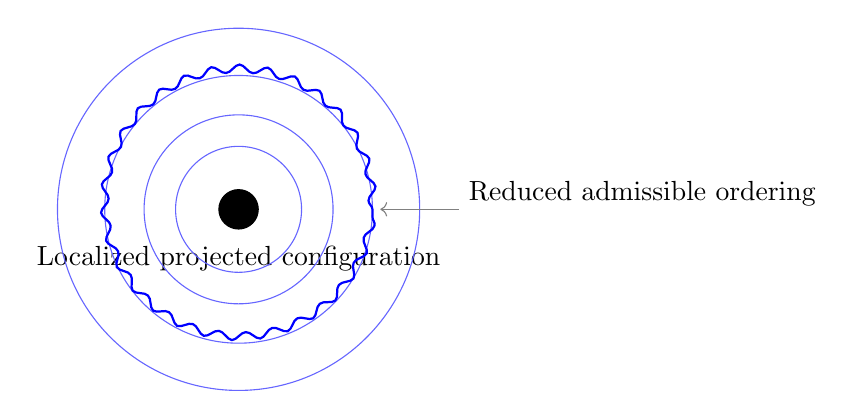
\begin{tikzpicture}[scale=1]

% Central mass
        \filldraw[black] (0,0) circle (0.25);
        \node[below] at (0,-0.35) {Localized projected configuration};

% Effective ordering contours
        \foreach \r in {0.8,1.2,1.7,2.3} {
          \draw[blue!60] (0,0) circle (\r);
        }

% Distortion
        \draw[blue, thick, decorate, decoration={snake, amplitude=0.5mm}]
        (0,0) circle (1.7);

% Arrows
        \draw[->, gray] (2.8,0) -- (1.8,0);
        \node[right] at (2.8,0.2) {Reduced admissible ordering};

      \end{tikzpicture}
      \caption
      {Emergence of Schwarzschild-like behavior in Cosmochrony.
      A localized projected configuration induces a spatially varying reduction of admissible relaxation ordering.
      In effective geometric descriptions, this manifests as differential proper-time
      accumulation and an emergent metric curvature analogous to gravitational time dilation.}
      \label{fig:chi_gravity}
    \end{figure}

  \input{07-gravity-as-a-collective-effect-of-particle-excitations/05-equivalence-principle}
  \input{07-gravity-as-a-collective-effect-of-particle-excitations/06-gravitational-waves}
  Before turning to strong-gravity regimes, it is useful to summarize the different
projective regimes discussed in this section.

\begin{figure}[h]
  \centering
  \begin{tabular}{c c c c c}
    \textbf{Projectable} &
    $\rightarrow$ &
    \textbf{Horizon} &
    $\rightarrow$ &
    \textbf{Non-projectable} \\[6pt]

    Gravitational &
    &
    Boundary of &
    &
    Deprojected \\
    Waves &
    &
    Projection &
    &
    Regime \\[6pt]

    Effective &
    &
    $\Pi$ non-injective &
    &
    No spacetime \\
    Modulations &
    &
    &
    &
    Representation
  \end{tabular}
  \caption{Conceptual regimes of projection in Cosmochrony.
  Gravitational waves correspond to fully projectable collective modulations of
  admissible descriptions, while black holes mark the boundary beyond which spacetime
  representations cease to be injective.
  Black hole evaporation reflects the gradual restoration of projectability,
    without any loss of information at the fundamental relational level,
    but only a loss and recovery of spacetime representability.}
  \label{fig:chi_projection_regimes}
\end{figure}

This schematic overview highlights how gravitational waves, horizons, and black hole
evaporation correspond to distinct regimes of projectability of the same underlying
relational structure.

\subsection{Strong Gravity and Black Holes}
  \label{subsec:strong-gravity-and-black-holes}

  In regions where the density of localized projected configurations becomes
  sufficiently high, admissible relaxation ordering becomes strongly constrained.
  In effective spacetime descriptions, this corresponds to a regime in which the local
  accumulation of effective time is strongly suppressed relative to distant observers,
  defining an effective horizon.

  Within Cosmochrony, such regions are interpreted as black holes.
  Rather than being characterized by a fundamental spacetime singularity, black holes
  correspond to domains where physical processes become asymptotically inaccessible
  from the exterior due to the loss of injectivity of spacetime projection.
  This naturally accounts for extreme time dilation effects without requiring divergent
  curvature invariants.

  These regions therefore mark not a terminal endpoint of physical description, but a
  transition toward a non-projectable regime of the underlying relational structure.

  \subsubsection*{Gravitational and Temporal Shadows}

    In the strong-gravity regime, the increasing concentration of localized projected
    configurations induces severe constraints on admissible ordering.
    As a result, the effective progression of time within the region slows
    asymptotically with respect to external descriptions.

    This behavior reproduces the phenomenon commonly referred to as a
    \emph{gravitational shadow}.
    In general relativity, such shadows arise from the absence of escaping null
    geodesics within a characteristic angular region.
    In Cosmochrony, an equivalent observational signature emerges because effective
    propagating descriptions, including radiation-like modes, no longer admit a faithful
    spacetime representation once projectability is lost.
    External observers therefore perceive a dark angular region corresponding to the
    projection of a non-projectable domain.

    Beyond this optical effect, the framework predicts a deeper phenomenon, which may be
    termed a \emph{temporal shadow}.
    As projectability is progressively lost, internal processes become indefinitely
    delayed in effective spacetime descriptions.
    From the external perspective, physical evolution appears frozen, providing a
    natural interpretation of horizon-induced time dilation.

    In this view, the observed gravitational shadow corresponds to the visible
    manifestation of an underlying temporal shadow.
    Both effects arise from the same loss of projective representability and do not
    require a fundamental spacetime singularity.

  \subsubsection*{Absence of Physical Singularities}

    In classical general relativity, black holes are associated with spacetime
    singularities characterized by divergent curvature and energy density.
    In Cosmochrony, such singularities are interpreted as artifacts of extending
    effective spacetime descriptions beyond their domain of validity.

    Because admissible ordering is bounded, configurations corresponding to infinite
    curvature or density cannot be physically realized.
    Apparent singularities therefore signal the breakdown of spacetime representability
    rather than genuine divergences of the underlying relational structure.

    \paragraph{Structural bound and notation.}
      To avoid confusion between fundamental and emergent levels, we distinguish the
      dimensionless structural bound $c_{\chi}$, defined at the level of the pre-geometric
      relational substrate, from its emergent spacetime manifestation $c$, interpreted as
      the maximal signal propagation speed.
      While $c$ may exhibit effective regime-dependent variations, the bound $c_{\chi}$ is
      invariant.

  \subsubsection*{Black Holes, Deprojection, and Vacuum Reprojection}
    \label{subsec:black-hole-deprojection-cycle}

    Within Cosmochrony, the absence of physical singularities does not imply that black
    holes are dynamically inert.
    Rather, they correspond to regimes in which the projection of relational information
    onto spacetime ceases to be injective.

    The emergence of an effective spacetime description relies on a projection map
    \[
      \Pi : \mathcal{C}_{\mathrm{rel}} \longrightarrow \mathcal{M},
    \]
    from the space of relational configurations to an effective spacetime manifold.
    In weak- and moderate-field regimes, this map is locally injective, ensuring a faithful
    geometric encoding.

    In strong-gravity regimes, this injectivity breaks down.
    Multiple inequivalent relational configurations correspond to the same effective
    spacetime event, signaling a loss of representability without any loss of information.
    We refer to this loss of injectivity as \emph{deprojection}.

    Deprojection does not correspond to transport across a spatial boundary nor to a
    temporal reversal.
    Instead, relational information ceases to be expressible in spatiotemporal form and
    remains encoded structurally.

    Importantly, deprojected information is not destroyed.
    Because the underlying relational configuration remains globally defined, information
    is in principle reprojectable once projectability is restored.
    Reprojection occurs discretely and manifests in effective spacetime descriptions as
    radiation-like excitations or particle--antiparticle pairs.

    The deprojection regime associated with black hole horizons does not imply the
    absence of dynamical processes.
    While smooth metric evolution ceases, the $\chi$ substrate remains structurally active.
    In particular, reprojection may occur intermittently when local configurations
    reach the threshold required for effective visibility.
    In the following section, this process is formalized through an explicit
    reprojection flux equation governing black hole evaporation.

    \paragraph{Information conservation and unitarity.}
      Deprojection does not correspond to information loss.
      It marks the loss of spacetime encoding, not the destruction of correlations.
      At the fundamental relational level, global information is preserved.
      Apparent non-unitarity arises only within projected spacetime descriptions and
      reflects their limited domain of applicability.

      This reprojection mechanism is analogous to vacuum fluctuations
      (Section~\ref{subsec:vacuum-fluctuations-and-the-casimir-effect}), where structural information is temporarily
      non-projectable before re-emerging as radiation.

  \subsection{Black Hole Evaporation and the Information Problem}
  \label{subsec:black-hole-evaporation-information}

  Within the Cosmochrony framework, black holes are not associated with physical
  singularities, but with regions where spacetime projection ceases to be injective.
  Such regions define domains of limited representability rather than physical interiors.

  \paragraph{Evaporation as a Projective Phenomenon.}
    Black hole evaporation is an effective process unfolding entirely within the
    projectable regime.
    It arises from the gradual restoration of projectability near the boundary separating
    projectable and non-projectable domains.

    As projectability is progressively recovered, localized projected configurations
    cease to be supported and are replaced by radiation-like effective descriptions.
    The evaporation process completes before any effective description would encounter a
    non-projectable singular regime.

  \paragraph{Resolution of the Information Paradox.}
    The apparent information loss identified by Hawking arises from treating spacetime as
    fundamental~\cite{Hawking1976}.
    In Cosmochrony, information is encoded in the global relational configuration
    independently of its spacetime projection.
    Evaporation therefore does not violate unitarity; it reflects a change in the domain
    of representability.

  \paragraph{Observational Implications.}
    To external observers, emitted radiation appears nearly thermal and weakly
    correlated with infalling states.
    This reflects the coarse-grained nature of spacetime projection rather than genuine
    information loss.
    The black hole information paradox is thus resolved by recognizing it as an artifact
    of extrapolating spacetime concepts beyond their domain of validity.

\subsubsection*{Horizon Reprojection Equation}
  \label{subsec:horizon-reprojection-equation}

  Within Cosmochrony, black hole evaporation is described as a reprojection process
  by which structural energy stored in the $\chi$ substrate is released into the projected
  spacetime in discrete units.

  The energy flux emerging from the horizon is defined as a sum over reprojection
  events associated with micro-configurations of the projection fiber:
  \[
    \Phi_\chi \equiv \frac{dE}{dt}
    = \sum_k \delta(t - t_k)\, \hbar_\chi\, \nu_k(L_{\mathrm{sol}}).
  \]

  Here, $\hbar_\chi$ denotes the fundamental quantum of reprojection, setting the
  minimal granularity of projected action.
  The quantities $\nu_k(L_{\mathrm{sol}})$ correspond to the resonance frequencies
  associated with the eigenmodes of the stability operator $L_{\mathrm{sol}}$ acting
  on the projection fiber $\Pi^{-1}(g_H)$ at the horizon, where $g_H$ denotes the
  effective near-horizon geometry.
  The times $t_k$ label the instants at which local $\chi$ configurations reach the
  projection threshold and become effectively visible in spacetime.

  Black hole evaporation thus proceeds as a sequence of discrete reprojection pulses,
  rather than as a continuous emission process.

\subsubsection*{Emergent Temperature and Relaxation Gradient}
  \label{subsec:emergent-temperature}

  The apparent Hawking temperature perceived by a distant observer emerges from the
  statistical distribution of reprojection events.
  It is determined by the gradient of effective $\chi$ relaxation normal to the horizon.

  This relation may be expressed as
  \[
    k_B T_\chi = \frac{\hbar_\chi c}{2\pi}\,
    \left| \nabla_{\perp} \chi_{\mathrm{eff}} \right|_H.
  \]

  For more massive black holes, the relaxation gradient is distributed over a larger
  horizon area, reducing the frequency of reprojection events.
  This directly explains the inverse mass–temperature relation without invoking
  vacuum particle creation or fundamental thermodynamic assumptions.

\subsubsection*{Information Conservation and Spectral Encoding}
  \label{subsec:information-conservation}

  In contrast with semiclassical descriptions, information is never destroyed in
  Cosmochrony.
  The projection operator $\Pi$ acts as a filter rather than as an irreversible map.

  During the deprojection phase, information is stored in the nonlinear degrees of
  freedom of the $\chi$ substrate, encoded within the projection fiber.
  During reprojection, the emitted radiation carries the precise spectral imprint of
  the eigenmodes governing the $\chi$ configuration.

  Each emitted quantum corresponds to a specific transition within the substrate,
  ensuring global unitarity.
  The apparent loss of information arises solely from restricting attention to the
  projected metric degrees of freedom.

\subsubsection*{Entropy as a Projection Saturation Limit}
  \label{subsubsec:entropy-projection-saturation}

  Within the Cosmochrony framework, the recovery of the Bekenstein--Hawking
  area law,
  \begin{equation}
    S = \frac{A}{4},
  \end{equation}
  does not rely on the introduction of a temperature or on thermodynamic
  postulates.
  Instead, black hole entropy is reinterpreted as a measure of the
  informational capacity of the projection map $\Pi$ at the horizon boundary.

  \paragraph{The Horizon as a De-projection Boundary}

    In the near-horizon regime, the $\chi$ substrate approaches a state of
    critical constraint in which the mapping
    \(
    \Pi : \chi \rightarrow g_{\mu\nu}
    \)
    ceases to be injective (see Section~7.7.3).
    The horizon is therefore redefined as the locus at which the local
    relaxation rate $N(r)$ vanishes, preventing further refinement of the
    projected metric degrees of freedom.

    At this boundary, distinct micro-configurations of the substrate are
    mapped onto the same effective horizon geometry $g_H$.
    Entropy is identified with the logarithmic measure of the fiber
    \(
    \Pi^{-1}(g_H),
    \)
    that is, the structural multiplicity of $\chi$ configurations that are no
    longer distinguishable at the metric level.
    Entropy thus quantifies hidden relational structure, rather than thermal
    ignorance.

    This situation is schematically illustrated in
    Figure~\ref{fig:projection-saturation-horizon}.

    \begin{figure}[htbp]
      \centering
      \resizebox{\linewidth}{!}{%
        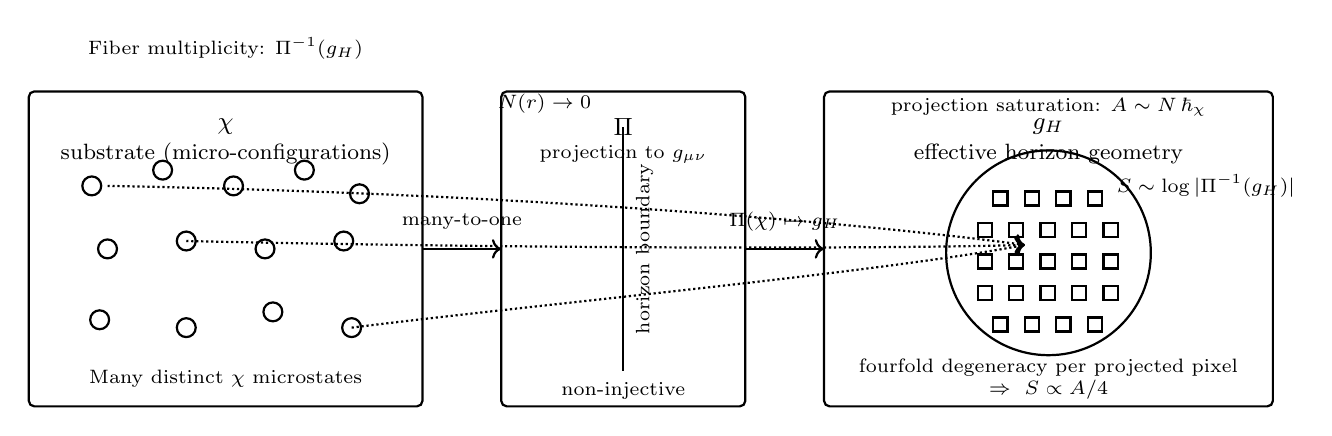
\begin{tikzpicture}[font=\small]

          % --- Geometry constants (implicit): boxes are placed in absolute coordinates ---
          % Left box: chi
          \draw[thick,rounded corners=2pt] (0,0) rectangle (5.0,4.0);
          \node at (2.5,3.55) {$\chi$};
          \node[font=\footnotesize] at (2.5,3.20) {substrate (micro-configurations)};

          % Middle box: projection / horizon boundary
          \draw[thick,rounded corners=2pt] (6.0,0) rectangle (9.1,4.0);
          \node at (7.55,3.55) {$\Pi$};
          \node[font=\scriptsize] at (7.55,3.20) {projection to $g_{\mu\nu}$};

          % Right box: g_H (keep minimal to avoid overlap)
          \draw[thick,rounded corners=2pt] (10.1,0) rectangle (15.8,4.0);
          \node at (12.95,3.55) {$g_H$};
          \node[font=\footnotesize] at (12.95,3.20) {effective horizon geometry};

          % --- Microstates (left box) ---
          \foreach \x/\y in {0.8/2.8,1.7/3.0,2.6/2.8,3.5/3.0,4.2/2.7,
          1.0/2.0,2.0/2.1,3.0/2.0,4.0/2.1,
          0.9/1.1,2.0/1.0,3.1/1.2,4.1/1.0}{
            \draw[thick] (\x,\y) circle (0.12);
          }
          \node[font=\scriptsize] at (2.5,0.35) {Many distinct $\chi$ microstates};

          % --- Arrow to middle box ---
          \draw[->,thick] (5.0,2.0) -- (6.0,2.0);
          \node[font=\scriptsize] at (5.5,2.35) {many-to-one};

          % --- Horizon boundary line inside middle box ---
          \draw[thick] (7.55,0.45) -- (7.55,3.55);
          \node[font=\scriptsize,rotate=90] at (7.82,2.0) {horizon boundary};
          \node[font=\scriptsize] at (6.55,3.85) {$N(r)\to 0$};
          \node[font=\scriptsize] at (7.55,0.20) {non-injective};

          % --- Arrow to right box ---
          \draw[->,thick] (9.1,2.0) -- (10.1,2.0);
          \node[font=\scriptsize] at (9.6,2.35) {$\Pi(\chi)\mapsto g_H$};

          % --- Horizon disk + pixels (right box) ---
          \draw[thick] (12.95,1.95) circle (1.30);
          \node[font=\scriptsize] at (12.95,3.80) {projection saturation: $A \sim N\,\hbar_\chi$};

          % pixels inside the disk (all are safely inside)
          \foreach \x/\y in {12.25/2.55,12.65/2.55,13.05/2.55,13.45/2.55,
          12.05/2.15,12.45/2.15,12.85/2.15,13.25/2.15,13.65/2.15,
          12.05/1.75,12.45/1.75,12.85/1.75,13.25/1.75,13.65/1.75,
          12.05/1.35,12.45/1.35,12.85/1.35,13.25/1.35,13.65/1.35,
          12.25/0.95,12.65/0.95,13.05/0.95,13.45/0.95}{
            \draw[thick] (\x,\y) rectangle ++(0.18,0.18);
          }

          % --- Dotted arrows: selected microstates collapse to same horizon pixel ---
          \draw[->,thick,densely dotted] (1.0,2.8) .. controls (6.5,2.7) and (10.8,2.3) .. (12.65,2.05);
          \draw[->,thick,densely dotted] (2.0,2.1) .. controls (6.5,2.0) and (10.8,2.0) .. (12.65,2.05);
          \draw[->,thick,densely dotted] (4.1,1.0) .. controls (6.5,1.3) and (10.8,1.7) .. (12.65,2.05);

          % --- External annotations (kept outside boxes to avoid overlap) ---
          \node[font=\scriptsize,align=left] at (2.5,4.55) {Fiber multiplicity: $\Pi^{-1}(g_H)$};
          \node[font=\scriptsize,align=left] at (14.95,2.80) {$S \sim \log |\Pi^{-1}(g_H)|$};
          \node[font=\scriptsize,align=center] at (12.95,0.35)
            {fourfold degeneracy per projected pixel\\$\Rightarrow\ S \propto A/4$};

        \end{tikzpicture}%
      } % resizebox

      \caption{
        Saturation of the projection map at the horizon.
        Near the boundary where $N(r)\to 0$, the projection $\Pi$ becomes non-injective:
        multiple micro-configurations of the $\chi$ substrate collapse onto the same
        effective horizon geometry $g_H$.
        Entropy measures the structural multiplicity of the fiber $\Pi^{-1}(g_H)$ and the
        saturation of projected metric ``pixels'' of area $\sim \hbar_\chi$.
      }
      \label{fig:projection-saturation-horizon}
    \end{figure}

  \paragraph{Geometric Origin of the \texorpdfstring{$1/4$}{1/4} Factor}

    The numerical factor $1/4$ arises as a structural ratio between the
    internal degrees of freedom of the $\chi$ substrate and their maximal
    holographic projection onto a two-dimensional boundary.

    Let $\hbar_\chi$ denote the elementary quantum of reprojection.
    The horizon area $A$ is saturated by a finite number $N$ of effective
    pixels of area $\sim \hbar_\chi$.
    Within the Cosmochrony framework, each such projected pixel corresponds to
    a fourfold degeneracy in the stability spectrum of $\chi$, linked to the
    intrinsic $4\pi$ periodicity of $\chi$ excitations discussed in
    Section~5.2.

    The area law
    \(
    S = A/4
    \)
    is therefore the macroscopic signature of this quadrature constraint:
    it represents the maximal density of independent structural degrees of
    freedom that can be projected before the non-injectivity of $\Pi$ induces
    a complete loss of local metric resolution.

  \paragraph{Unitary Reprojection and Information Conservation}

    Black hole evaporation is reformulated as a discrete reprojection
    process.
    As the $\chi$ substrate locally relaxes at the horizon boundary, it emits
    quanta of action $\hbar_\chi$ carrying the spectral imprint of the fiber
    $\Pi^{-1}(g_H)$.

    Because this process is governed by the deterministic---though
    nonlinear---relaxation dynamics of $\chi$, information is never destroyed
    nor trapped in a singularity.
    Instead, it is transferred from a purely structural encoding within the
    fiber back into observable spacetime degrees of freedom.
    Unitarity is preserved at the level of the $\chi$ substrate, even though
    the effective spacetime description may exhibit apparent non-unitarity.

  \paragraph*{Conclusion}

    In Cosmochrony, black hole entropy is not a measure of ignorance but a
    measure of projection saturation.
    It quantifies the threshold at which the complexity of the $\chi$
    substrate exceeds the transmittance capacity of the effective metric
    projection.
    This explains why entropy scales with area---the projection surface---and
    not with volume, which characterizes the inaccessible internal fiber.

  \input
  {07-gravity-as-a-collective-effect-of-particle-excitations/09-unified-origin-of-gravitational-and-electromagnetic-effects}
  \subsection{Summary}
  \label{subsec:summary6}

  Within the Cosmochrony framework, gravity does not arise as a fundamental interaction
  or as an independent geometric degree of freedom.
  It emerges at the level of effective descriptions as a macroscopic consequence of
  localized projected configurations collectively constraining admissible relaxation
  ordering.

  Classical gravitational phenomena—including gravitational time dilation, effective
  spacetime curvature, gravitational waves, and black holes—are recovered as distinct
  descriptive regimes of this collective constraint.
  They reflect variations in the projectability and correlation structure of admissible
  descriptions, rather than the dynamics of a fundamental spacetime or gravitational
  field.

  In this perspective, gravitation appears as an emergent, operational phenomenon,
  summarizing how localized projected configurations collectively limit admissible
  ordering and correlation across extended regions, without introducing gravity as a
  primitive force or fundamental geometric entity.


  \section{Quantum Phenomena and Entanglement}
  \label{sec:quantum-phenomena-and-entanglement}

  \subsection{Nonlocality and the Holistic Nature of the $\chi$ Field}
    \label{subsec:nonlocality-and-holistic-nature}

    In the Cosmochrony framework, quantum nonlocality does not arise from superluminal
    interactions or from violations of relativistic causality~\cite{Bell1964}.
    Instead, it reflects the intrinsically holistic nature of the $\chi$ field.
    Entangled systems correspond to single, extended configurations of $\chi$ that
    cannot be factorized into independent subsystems once they have interacted.

    The persistence of quantum correlations across spatial separation follows from
    the internal relational structure of $\chi$, rather than from spatial connectivity
    or signal exchange.
    Although effective geometric descriptions may assign distant locations to parts
    of an entangled system, these locations correspond to different manifestations of
    a single underlying field configuration.

    In this sense, quantum nonlocality in Cosmochrony is ontological rather than
    dynamical: the field configuration is globally defined, while its evolution
    remains locally governed by the relaxation dynamics of $\chi$.

    This holistic character of $\chi$ plays a crucial role in quantum measurement.
    Because entangled systems correspond to a single, non-factorizable configuration,
    measurement outcomes cannot be understood as revealing pre-existing local
    properties.
    Instead, decoherence acts to suppress relational alternatives within a globally
    defined configuration, while local measurement outcomes correspond to effective
    reprojections selected by fluctuations.

    In this context, the Born rule does not encode nonlocal influence or hidden
    communication.
    It reflects the statistical distribution of locally accessible outcomes arising
    from a single holistic configuration of $\chi$, once relational coherence has been
    lost.
    Nonlocal correlations therefore arise from global structural consistency, while
    measurement statistics remain compatible with relativistic causality.

    Crucially, this global configuration does not encode predetermined measurement
    outcomes, but only a space of structurally compatible relational realizations,
    whose effective selection occurs through decoherence and reprojection.

  \subsection{Shared Configurations and Correlation Structure}
    \label{subsec:shared-configurations}

    When two particle-like excitations interact, they may form a composite
    configuration of the $\chi$ field that remains partially unified even after
    spatial separation in an effective geometric description.
    Such configurations give rise to persistent correlations between measurement
    outcomes.

    In an effective spacetime representation, this shared configuration may be
    schematically modeled as
    \begin{equation}
      \chi(x) = \chi_0 \exp\!\left(
                               -\frac{|x - x_1|^2}{\xi^2}
                               -\frac{|x - x_2|^2}{\xi^2}
      \right),
    \end{equation}
    where $x_1$ and $x_2$ label the effective locations of the two excitations.
    This expression is not fundamental, but serves as an illustrative coarse-grained
    representation of a single extended $\chi$ excitation whose internal structure
    spans multiple regions.

    The observed quantum correlations arise because measurements performed on
    different parts of this unified configuration probe the same underlying relational
    state, rather than because of any exchange of signals at the time of measurement.

  \subsection{Nonlocal Correlations Without Superluminality}
    \label{subsec:nonlocal-correlations-without-superluminality}

    Because the $\chi$ field evolves locally according to its relaxation dynamics,
    no superluminal propagation of information occurs.
    Measurement outcomes at spacelike separated regions do not influence one another
    through causal signals.

    Instead, correlated outcomes arise because both measurements sample the same
    pre-existing relational structure of $\chi$.
    This violates the factorization assumptions underlying Bell-type inequalities,
    while preserving dynamical locality and relativistic causality.

    In this way, Cosmochrony naturally accounts for experimentally observed violations
    of Bell inequalities without invoking nonlocal forces, retrocausality, or hidden
    signal channels.

  \subsection{Measurement, Decoherence, and Apparent Collapse}
    \label{subsec:measurement-and-decoherence}

    Within Cosmochrony, quantum measurement does not involve a fundamental wavefunction
    collapse.
    The $\chi$ field evolves continuously according to its intrinsic dynamics, and no
    discontinuous update of the underlying configuration occurs.

    What is conventionally interpreted as wavefunction collapse corresponds to the
    loss of coherence between different components of a $\chi$ configuration due to
    interaction with an environment.
    This process dynamically suppresses interference between alternative relational
    branches, yielding effectively classical outcomes.

    Decoherence therefore arises as a physical process rooted in the coupling between
    localized excitations and the broader $\chi$ field, rather than as a postulated
    measurement axiom~\cite{Zurek2003}.

    Importantly, decoherence does not destroy information at the level of the $\chi$
    substrate.
    Rather, it suppresses the relational accessibility of phase information within
    emergent spacetime.
    In this sense, decoherence may be viewed as a local and partial form of
    deprojection: relational histories become dynamically inaccessible while the
    underlying structural configuration of $\chi$ remains unchanged.

    More extreme regimes, such as those associated with strong gravitational
    confinement, represent a limiting case of this mechanism.
    There, relational and spatiotemporal descriptions themselves cease to be
    maintainable, and information undergoes full deprojection into the $\chi$
    substrate, beyond the domain where decoherence is defined.

  \subsection{Temporal Ordering and Relativistic Consistency}
    \label{subsec:temporal-ordering-and-relativistic-consistency}

    Because temporal ordering in Cosmochrony is defined by the monotonic relaxation of
    $\chi$, it does not rely on a global simultaneity structure.
    Different observers may assign different temporal orderings to spacelike separated
    events in effective geometric descriptions, without affecting the underlying
    dynamics of the field.

    Entanglement correlations are therefore compatible with relativistic causality:
    they do not depend on any preferred reference frame or absolute notion of time.
    The relational structure of $\chi$ remains invariant under changes of effective
    spacetime slicing.

  \subsection{Limits of Entanglement and Environmental Effects}
    \label{subsec:limits-of-entanglement}

    Entanglement is not a generic or permanent feature of all $\chi$ configurations.
    Environmental interactions, noise, and continued relaxation progressively degrade
    the coherence of shared configurations.

    As a result, entanglement is most robust for isolated systems and diminishes in
    macroscopic or strongly interacting environments.
    This explains the emergence of classical behavior at large scales without
    requiring a fundamental quantum-to-classical transition.

  \subsection{Summary}
    \label{subsec:summary8}

    Entanglement emerges in Cosmochrony as the persistence of shared topological
    configurations within the $\chi$ field.
    Quantum correlations arise without superluminal signaling, fundamental wavefunction
    collapse, or violations of relativistic causality.

    Within this framework, quantum phenomena reflect the holistic yet dynamically local
    structure of $\chi$, from which the standard quantum-mechanical formalism emerges
    as an effective statistical description rather than a fundamental ontology.

  \section{Relation to Quantum Formalism}
  \label{sec:relation-to-quantum-formalism}

  This section does not assign fundamental ontological status to the quantum
  wavefunction, Hilbert space, or operator structures.
  Instead, it shows how the formal apparatus of quantum mechanics arises as an
  effective and internally consistent description organizing admissible projected
  descriptions in regimes where localization, linearity, and approximate
  factorization hold.

  Within the Cosmochrony framework, quantum mechanics is not derived from an
  underlying microscopic dynamics of the $\chi$ substrate.
  Rather, it emerges as a universal coarse-grained formalism governing the
  projectability and temporal consistency of localized physical descriptions once a
  stable geometric interpretation becomes applicable.

  Quantum mechanics is therefore not replaced, but reinterpreted as an effective
  framework whose validity is restricted to regimes where the relational structure
  of $\chi$ admits a stable, approximately linear, spacetime-based description.
  The following subsections clarify the origin and interpretational status of the
  wavefunction, Hilbert space structure, quantization, measurement, entanglement,
  and related quantum concepts within this perspective.

  \subsection{Status of the Wavefunction}
  \label{subsec:status-of-the-wavefunction}

  In standard quantum mechanics, the wavefunction $\psi$ is a complex-valued object
  defined on configuration space, whose ontological status remains debated.
  Operationally, $|\psi|^2$ encodes measurement probabilities via the Born rule, while
  $\psi$ itself does not correspond to a physical field propagating in spacetime.

  Within the Cosmochrony framework, the quantum wavefunction is not identified with any
  fundamental physical entity.
  It arises at the level of effective descriptions as a statistical encoding of the
  set of admissible local reprojections compatible with a given non-factorizable
  projected configuration.

  The wavefunction therefore does not represent an underlying structure or hidden
  dynamics.
  It summarizes, in compact mathematical form, the relative accessibility of different
  local outcomes once a global descriptive coherence has been established.
  Its complex phase encodes relational constraints between alternative local
  descriptions, while its modulus determines the statistical weight of accessible
  reprojections.

  As an illustrative example, the hydrogen atom wavefunctions
  $\psi_{nlm}(r,\theta,\phi)$ do not correspond to localized structures or solitonic
  configurations at a fundamental level.
  They represent stationary admissible projected descriptions characterized by
  specific symmetry and stability properties.
  The probability density $|\psi|^2$ reflects the relative frequency with which
  localized reprojections occur in effective geometric descriptions, while energy
  quantization arises from the discrete admissibility conditions imposed on stationary
  descriptive regimes.

  In this perspective, the wavefunction is neither a physical field nor a direct image
  of an underlying substrate.
  It is a derived statistical object, encoding the structure of admissible projected
  descriptions and the probabilities of their local realization within spacetime.

  \subsection{Emergence of Hilbert Space Structure}
  \label{subsec:emergence-of-hilbert-space-structure}

  The Hilbert space formalism of quantum mechanics provides a linear structure
  supporting superposition, interference, and unitary evolution.
  Within the Cosmochrony framework, this structure does not reflect a fundamental
  property of an underlying physical substrate.
  It emerges as an effective mathematical organization of admissible projected
  descriptions in regimes where relational constraints are weak and approximately
  factorizable.

  In such regimes, distinct admissible projected descriptions can be combined without
  significant mutual constraint, giving rise to an approximate linear structure.
  Superposition reflects the coexistence of multiple compatible descriptive
  alternatives, rather than the simultaneous physical realization of multiple states.

  The inner-product structure of Hilbert space encodes the degree of mutual
  compatibility between projected descriptions.
  Orthogonality corresponds to mutually exclusive descriptive regimes, while
  non-orthogonal states represent partially compatible projections whose distinctions
  cannot be jointly resolved.

  The complex phase of the wavefunction does not correspond to an intrinsic oscillatory
  structure of a physical field.
  It encodes relational consistency conditions between alternative projected
  descriptions, ensuring coherent interference patterns within effective spacetime
  representations.

  Unitary evolution arises as a consistency-preserving transformation within the space
  of admissible projected descriptions, valid so long as projectability and
  factorizability remain approximately intact.
  When these conditions fail, such as during measurement or strong environmental
  coupling, the Hilbert space description ceases to be adequate, and non-unitary
  effective behavior emerges.

  In this perspective, Hilbert space is not a fundamental arena of physical reality.
  It is the natural mathematical structure organizing the space of admissible
  descriptions in regimes where linearity and coherence provide accurate effective
  approximations.

  \subsection{Emergence of the Schr\"odinger Equation as an Effective Description}
  \label{sec:schrodinger_emergence}

  Within the Cosmochrony framework, quantum dynamics is not postulated as a fundamental
  law.
  The Schr\"odinger equation arises as an effective, long-wavelength and
  non-relativistic description organizing admissible projected descriptions in regimes
  where localization, approximate factorization, and temporal projectability are
  simultaneously valid.

  Rather than emerging from physical fluctuations of an underlying field, the
  Schr\"odinger equation appears as the universal consistency condition governing the
  time evolution of localized projected descriptions whose internal structure remains
  approximately stationary.

  \subsubsection*{Formal Non-Relativistic Limit}
    \label{sec:KGtoSch}

    In regimes where an effective relativistic description applies, admissible projected
    descriptions of localized configurations admit a second-order hyperbolic evolution
    equation whose formal structure coincides with the Klein--Gordon equation.
    This equation should be understood as an effective geometric encoding of stability
    and admissibility conditions, not as a fundamental field equation.

    In the non-relativistic regime, the effective description separates naturally into a
    rapidly varying phase associated with rest-energy and a slowly varying envelope
    describing spatial localization.
    Formally, this separation may be written as
    \begin{equation}
      \Psi(x,t) = \psi(x,t)\, e^{-i \omega_0 t},
      \qquad \omega_0 = \frac{mc^2}{\hbar},
    \end{equation}
    where $\Psi$ denotes an effective relativistic descriptive field and $\psi$ its
    non-relativistic envelope.

    Imposing the condition that the envelope varies slowly compared to the rest-energy
    scale leads, to leading order, to the Schr\"odinger equation,
    \begin{equation}
      i\hbar\,\partial_t \psi
      = -\frac{\hbar^2}{2m}\nabla^2 \psi + V(x)\psi,
      \label{eq:Sch_V}
    \end{equation}
    where $V(x)$ encodes weak external constraints on admissible projected descriptions,
    such as background gravitational or electromagnetic effects.

    \paragraph{Interpretation.}
      The wavefunction $\psi$ does not represent a physical excitation or fluctuation of an
      underlying substrate.
      It is a derived mathematical object encoding the admissible time evolution of
      localized projected descriptions once a non-relativistic spacetime interpretation
      becomes applicable.

      In this sense, the Schr\"odinger equation is not a fundamental dynamical law.
      It is the effective evolution equation governing admissible projected descriptions in
      regimes where linearity, localization, and approximate factorization provide accurate
      descriptive approximations.

  \subsection{Origin of Quantization}
  \label{subsec:origin-of-quantization}

  In standard quantum theory, quantization is introduced axiomatically through canonical
  commutation relations or path-integral prescriptions.
  Within the Cosmochrony framework, quantization is not fundamental and does not arise
  from an underlying microscopic dynamics.
  It emerges as a structural consequence of stability, consistency, and admissibility
  constraints imposed on projected descriptions.

  Only a restricted class of localized projected configurations admits long-lived,
  internally consistent descriptions.
  Configurations that fail to satisfy these constraints rapidly lose projectability
  and cannot be maintained as persistent physical descriptions.
  As a result, admissible configurations form discrete equivalence classes rather than
  a continuous spectrum.

  Energy quantization reflects this discreteness.
  Energy does not label an intrinsic property of a physical excitation, but characterizes
  the degree of structural persistence of a projected configuration within the relaxation
  ordering.
  Only specific values correspond to stable descriptive regimes, leading to an effective
  discretization of energy exchanges.

  The relation
  \begin{equation}
    E = h \nu
  \end{equation}
  does not express a fundamental oscillatory dynamics.
  It encodes a proportionality between the energetic cost of maintaining a persistent
  projected configuration and the characteristic ordering rate at which its internal
  structure must be consistently re-identified.
  The frequency $\nu$ should therefore be understood as a descriptive rate associated
  with relational re-identification, not as oscillation with respect to a fundamental
  time parameter.

  Within this perspective, Planck’s constant does not represent a fundamental quantum
  of action.
  It emerges as a universal conversion factor characterizing the minimal structural
  scale at which projected descriptions remain stable and coherent across ordering.
  Its apparent universality reflects the universality of the projectability constraints
  themselves, rather than the postulation of an underlying quantized substrate.

  \subsection{Measurement and the Born Rule}
  \label{subsec:measurement-and-the-born-rule}

  Within the Cosmochrony framework, measurement does not involve a fundamental
  wavefunction collapse, nor does it rely on stochastic fluctuations of an underlying
  physical substrate.
  The $\chi$ field evolves continuously and deterministically according to its intrinsic
  relational structure.

  What is conventionally described as a measurement corresponds to an irreversible
  loss of projectability: a localized projected description becomes dynamically coupled
  to a macroscopic environment, preventing the continued joint maintenance of
  incompatible relational alternatives.
  This process is described at the effective level by decoherence, as discussed in
  Section~\ref{subsec:measurement-and-decoherence}.

  Measurement outcomes correspond to effective reprojections onto mutually exclusive
  descriptive regimes.
  These outcomes are not selected by hidden fluctuations or random microscopic events,
  but by the structural compatibility between the pre-measurement description and the
  macroscopic constraints imposed by the measurement apparatus.

  The Born rule does not encode a fundamental probability law.
  It emerges as the unique stable measure on the space of admissible projected
  descriptions that remains invariant under loss of phase coherence and coarse-graining.
  The squared amplitude $|\psi|^2$ quantifies the relative measure of descriptive
  compatibility between a pre-measurement state and the set of macroscopically
  distinguishable outcomes.

  In this sense, $|\psi|^2$ does not represent subjective uncertainty or intrinsic
  randomness.
  It characterizes the structural weight of admissible reprojections consistent with
  both the prior relational configuration and the constraints defining the measurement
  context.
  The Born rule therefore reflects a geometric and consistency-based property of
  projected descriptions, rather than a fundamental stochastic law of nature.

  \subsection{Entanglement and Nonlocal Correlations}
  \label{subsec:entanglement-and-nonlocal-correlations}

  Within the Cosmochrony framework, quantum entanglement does not correspond to a
  physical linkage or interaction between spatially separated entities.
  It reflects the persistence of a shared relational structure within a single,
  non-factorizable configuration of the $\chi$ substrate.

  Entangled systems are described by projected configurations that cannot be
  decomposed into independent subsystems without loss of relational consistency.
  Although effective spacetime descriptions assign distinct locations to the
  corresponding subsystems, these locations represent different projections of a
  single underlying relational configuration.

  Nonlocal correlations therefore do not arise from superluminal influences or hidden
  signal exchange.
  They follow from the fact that measurement operations act on a globally defined
  relational structure whose admissible projections must remain mutually consistent.
  Once a projection is selected in one region, the set of admissible projections
  elsewhere is correspondingly constrained, without any dynamical transmission.

  In this sense, quantum nonlocality in Cosmochrony is ontological rather than
  dynamical.
  The underlying relational configuration is globally defined, while its evolution
  and reprojection remain locally governed by the relaxation and projectability
  constraints of $\chi$.
  As a result, entanglement correlations are fully compatible with relativistic
  causality and do not require the introduction of nonlocal forces or preferred
  reference frames.

  \subsection{Spin and Statistics}
  \label{subsec:spin-statistics}

  Within the Cosmochrony framework, spin does not arise as an intrinsic kinematic
  degree of freedom of a particle, nor as a fundamental representation of spacetime symmetries.
  Instead, it emerges as a topological property of admissible projected configurations associated with localized
  physical descriptions.

  Certain classes of admissible configurations possess a non-trivial internal covering
  structure such that a $2\pi$ effective rotation does not return the configuration to an
  equivalent descriptive state, while a $4\pi$ rotation does.
  Projected descriptions exhibiting this property correspond to fermionic behavior, whereas configurations
  that are $2\pi$-periodic correspond to bosonic behavior.

  The connection between spin and statistics follows directly from this topological distinction.
  Configurations with non-trivial covering structure cannot be symmetrically
  exchanged without violating relational consistency, leading to antisymmetric exchange behavior.
  By contrast, configurations with trivial topology admit symmetric exchange.

  Spin and statistics are therefore not independent postulates of quantum theory.
  They reflect the same underlying topological constraints on the space of admissible projected descriptions.
  This unified origin accounts simultaneously for half-integer spin, fermionic statistics, and the Pauli exclusion
  principle, without introducing additional quantum axioms.

  A concrete topological construction illustrating these properties is presented in
  Appendix~\ref{subsec:4pi_soliton}.

  \subsection{Orbital Geometry as Probabilistic Visibility}
  \label{sec:orbital_geometry_visibility}

  Atomic orbitals do not represent spatially extended material distributions.
  Within the Cosmochrony framework, they correspond to probabilistic visibility
  patterns associated with admissible projected descriptions of localized bound
  configurations.

  Orbital shapes encode structural and symmetry constraints imposed on admissible
  projected descriptions, such as nodal surfaces and angular dependence.
  These features reflect conditions of relational consistency and stability rather
  than the presence of a spatially distributed object.

  The apparent spatial extent of an orbital does not indicate the physical size or
  motion of an underlying entity.
  It reflects the range of effective spatial locations over which a projected
  description remains admissible under repeated reprojection and measurement.
  Regions of high probability correspond to domains where consistent reprojection is
  most robust, while nodal regions correspond to incompatible descriptive regimes.

  Orbital visualizations therefore do not depict occupied regions of space.
  They represent statistical maps of descriptive accessibility within an effective
  geometric representation.
  In this sense, atomic orbitals encode how bound configurations can be consistently
  described in spacetime, rather than revealing the spatial structure of an underlying
  physical object.

  \subsection{Scope and Limitations}
  \label{subsec:scope-and-limitations}

  Cosmochrony does not aim to replace quantum mechanics as a predictive or
  computational framework.
  All standard quantum-mechanical formalisms, including operator methods, path
  integrals, and perturbative techniques, remain valid and unchanged within their
  established domains of applicability.

  The contribution of Cosmochrony is interpretative and unificatory.
  It provides a coherent pre-geometric and relational origin for quantum phenomena,
  clarifying the ontological status of the wavefunction, quantization, measurement,
  and nonlocal correlations, without altering any experimentally verified
  predictions.

  In this framework, quantum mechanics is understood as an effective theory
  governing admissible projected descriptions in regimes where linearity,
  localization, and factorization hold approximately.
  Cosmochrony does not introduce new degrees of freedom, hidden variables, or
  modifications of quantum dynamics.

  A complete formal correspondence between the relational $\chi$ substrate and the
  operator-based structures of quantum theory, including a systematic derivation of
  Hilbert space, observables, and evolution operators, lies beyond the scope of the
  present work and is left for future investigation.

  Accordingly, the present framework should be regarded as a foundational
  reconstruction rather than a competing physical theory, intended to clarify the
  conceptual origin and domain of validity of quantum-mechanical descriptions.


  \section{Cosmological Implications}
  \label{sec:cosmology}

  \subsection{The Big Bang as a Maximal Constraint Regime of the $\chi$ Substrate}
  \label{subsec:big-bang-maximal-constraint}

  Within the Cosmochrony framework, the Big Bang is not interpreted as a spacetime singularity, nor as a physical event
  occurring at a definite moment.
  It corresponds instead to a limiting regime in which the relational structure of the $\chi$ substrate is maximally
  constrained.

  In this regime, the density of structural and topological constraints within $\chi$
  is such that no stable geometric projection is admissible~\cite{Einstein1915,Weinberg1972}.
  Concepts such as spatial distance, temporal duration, curvature, or causal ordering are therefore undefined.
  The apparent singular behavior encountered in standard cosmological models reflects the breakdown of effective
  spacetime descriptions when extrapolated beyond their domain of validity.

  Cosmic evolution is interpreted as the progressive relaxation of these maximal constraints.
  As the relational structure of $\chi$ becomes less constrained, increasingly stable projected descriptions become
  admissible, allowing effective notions of space, time, and geometry to emerge~\cite{Penrose1989Weyl}.
  The Big Bang thus marks not the beginning of spacetime, but the boundary beyond which spacetime ceases to be a
  meaningful descriptive framework.

  Within this perspective, the arrow of time does not originate from special initial conditions or entropy
  assumptions~\cite{Prigogine1997,Rovelli1991}.
  It arises intrinsically from the monotonic relaxation ordering of $\chi$away from the maximally constrained regime.
  Temporal ordering is therefore a consequence of the structural
  evolution of the substrate itself, rather than a feature imposed at the level of effective cosmological descriptions.

  \subsection{Cosmological Cycles of Constraint and Reprojection}
  \label{subsec:cosmic-reprojection-cycle}

  The maximally constrained regime identified with the Big Bang should not be
  interpreted as a unique or irreproducible event.
  It corresponds instead to a limiting configuration of the $\chi$ substrate in which
  structural constraints dominate to the extent that no stable spacetime projection
  is admissible.

  As global relaxation proceeds, increasingly stable projected descriptions become
  possible, giving rise to emergent spacetime, matter configurations, and large-scale
  cosmological structure.
  However, this maximal constraint regime is not confined to the early universe.
  It may be locally reapproached whenever structural constraints on $\chi$ saturate,
  most notably in regions of extreme gravitational confinement identified as black
  holes.

  In such regions, effective spacetime descriptions progressively lose validity.
  Relational information encoded in emergent degrees of freedom ceases to remain
  expressible within spacetime and undergoes deprojection into the purely relational
  $\chi$ substrate.
  This process does not destroy information but renders it inaccessible to spacetime
  descriptions.

  Crucially, deprojection does not imply irreversibility at the level of the substrate.
  As structural constraints relax, the same relational content may again admit
  admissible projected descriptions.
  Reprojection should therefore be understood not as a discrete physical process,
  but as the restoration of descriptive projectability once relational consistency
  conditions are satisfied.

  From this perspective, phenomena commonly associated with the quantum vacuum reflect
  the persistent presence of reprojectable relational structures within $\chi$, rather
  than the activity of fluctuating fields.
  The vacuum is not empty, but represents a regime of minimal yet non-vanishing
  projectability.

  Cosmological evolution in Cosmochrony thus involves a continuous interplay between
  global relaxation, local reconfinement, deprojection, and reprojection across scales.
  The universe is not characterized by a single origin or terminal state, but by
  recurrent transitions between regimes of descriptive admissibility and breakdown.

  \subsection{Cosmic Expansion Without Inflation}
  \label{subsec:expansion-without-inflation}

  In standard cosmology, an inflationary phase is introduced to account for the observed large-scale homogeneity,
  isotropy, and near-flatness of the universe, as well as to resolve the horizon problem~\cite{Guth1981,Linde1982}.
  Within the Cosmochrony framework, these features do not require a distinct inflationary epoch.

  At the pre-geometric level, the relational structure of the $\chi$ substrate is not organized according to spatial
  separation or causal horizons.
  Prior to the emergence of a stable geometric projection, notions such as distance, light cones, and causal
  disconnection are undefined.
  As a result, the conditions that give rise to the ``horizon problem'' in standard spacetime-based cosmology do not
  apply.

  Large-scale homogeneity and isotropy therefore reflect the global relational coherence of the $\chi$
  substrate in the maximally constrained regime, rather than the outcome of a rapid expansion of spacetime.
  When geometric descriptions become admissible, this coherence is inherited as initial large-scale regularity in the
  emergent spacetime.

  Cosmic expansion itself is interpreted as the progressive relaxation of relational constraints, leading to
  increasing effective separation between projected regions.
  This expansion does not correspond to motion through space, but to the gradual unfolding of geometric distinctions as
  ``projectability'' improves.

  The present framework does not aim to reproduce inflationary scenarios at the level of
  field-driven perturbation spectra.
  Instead, it redefines the origin and interpretation of primordial regularities and
  correlations as structural features of the relaxation and projection process itself.
  While a fully quantitative treatment of emergent anisotropies requires further
  spectral and numerical development, no distinct inflationary phase or additional
  dynamical degrees of freedom are invoked.

  \subsection{Cosmic Expansion as $\chi$ Relaxation}
  \label{subsec:expansion-as-relaxation}

  In the Cosmochrony framework, cosmic expansion does not correspond to the motion of matter through a pre-existing
  space~\cite{Friedmann1922}.
  It reflects instead the progressive relaxation of the relational $\chi$
  substrate, from which effective spatial distinctions and separations gradually emerge.

  As the ordering parameter associated with $\chi$
  increases monotonically, projected descriptions admit an ever larger range of mutually distinguishable regions.
  What is described in effective cosmological models as the ``expansion of space'' thus corresponds to the
  increasing projectability of relational differences within $\chi$, rather than to a dynamical stretching of a
  fundamental metric background.

  In this interpretation, expansion is not driven by an external energy component or a specific cosmological fluid.
  It is an intrinsic consequence of the relaxation ordering of the substrate itself.
  Localized matter configurations act as persistent structural constraints on this relaxation, leading to spatially
  inhomogeneous unfolding that later manifests, in effective geometric descriptions, as large-scale structure.


  Cosmic expansion is therefore reinterpreted as a geometric and relational phenomenon, emerging from the intrinsic
  evolution of $\chi$ and acquiring a spacetime interpretation only once a stable geometric regime becomes applicable.

  \subsection{Emergent Hubble Law}
  \label{subsec:emergent-hubble-law}

  In homogeneous regimes, the relaxation ordering of the relational $\chi$ substrate is uniform.
  When described using an effective cosmological time parameter $t$, introduced as a convenient label of the relaxation
  ordering, this uniform regime admits the linear representation:
  \begin{equation}
    \chi(t) = \chi_0 + c\, t .
  \end{equation}
  This expression does not define a fundamental time evolution, but provides an effective parametrization of cumulative
  relaxation in a homogeneous cosmological regime.

  Identifying effective spatial scales with accumulated relational differentiation in $\chi$
  leads naturally to a ``Hubble-like law'' relating relative separation rates to separation
  itself~\cite{Hubble1929,Hogg1999}.
  Within this effective description, the Hubble parameter may be written as:
  \begin{equation}
    H(t) \equiv \frac{1}{\chi}\,\frac{d\chi}{dt},
  \end{equation}
  where the derivative is understood as an effective rate with respect to the cosmological time parameter, not as a
  fundamental dynamical derivative.

  In this perspective, no independent scale factor or expansion field is required.
  The Hubble parameter emerges as a dimensionless measure of the global relaxation rate of $\chi$ relative to its
  accumulated value.

  The present-day Hubble constant $H_0$ is therefore interpreted as an effective observable quantifying the current
  state of global relaxation, rather than as a fundamental constant governing the dynamics of spacetime itself.

  \subsection{Cosmic Acceleration Without Dark Energy}
  \label{subsec:acceleration-without-dark-energy}

  Within the Cosmochrony framework, the observed late-time cosmic acceleration does not
  require the introduction of a cosmological constant or a dark energy component.
  No additional energy density or repulsive interaction is postulated at the
  fundamental level.

  The apparent acceleration arises as an effective consequence of the cumulative
  relaxation history of the relational $\chi$ substrate.
  As cosmic evolution proceeds, the formation of localized and long-lived structures
  (such as galaxies and clusters) increasingly constrains the local relaxation of
  $\chi$.
  These constraints introduce growing spatial inhomogeneities in the relaxation
  process.

  When interpreted within standard spacetime-based cosmological models, which assume
  a homogeneous and isotropic expansion driven by a global scale factor, these
  inhomogeneities manifest as an apparent acceleration of cosmic expansion.
  The effect reflects a mismatch between the underlying relational relaxation dynamics
  and the assumptions built into effective geometric descriptions.

  In this sense, cosmic acceleration is not a dynamical phenomenon requiring a new
  source of energy.
  It is an emergent, interpretative effect arising from the progressively uneven
  relaxation of $\chi$ across cosmic scales.
  As structure formation proceeds, the effective expansion inferred from observations
  naturally departs from the predictions of homogeneous models, without invoking dark
  energy.

  This interpretation aligns with approaches that attribute late-time acceleration to
  backreaction effects, while providing a unified and pre-geometric origin rooted in
  the relaxation dynamics of the $\chi$ substrate.

  \subsection{Cosmic Microwave Background}
  \label{subsec:cmb}

  Within the Cosmochrony framework, the cosmic microwave background (CMB) does not
  encode primordial fluctuations generated during a distinct inflationary phase.
  It reflects instead the imprint of early relaxation and reprojection processes as
  the relational $\chi$ substrate transitioned toward a regime admitting stable
  geometric descriptions.

  At this stage, the universe was not yet structured by well-defined spatial
  separation or causal horizons.
  Large-scale correlations observed in the CMB therefore arise naturally from the
  global relational coherence of $\chi$ prior to geometric differentiation, rather
  than from superluminal expansion within spacetime.

  The acoustic features observed in the temperature power spectrum admit an effective
  interpretation as resonance patterns arising during the transition to a stable
  geometric regime.
  They reflect the coupling between emerging matter configurations and the
  relaxation dynamics governing admissible projected descriptions, rather than
  oscillations of a fundamental physical field~\cite{SachsWolfe1967,HuWhite1997}.

  In this perspective, the CMB encodes a fossil record of the emergence of spacetime
  itself.
  Its large-angle correlations and statistical properties are consequences of the
  pre-geometric relational structure of $\chi$, inherited by the emergent spacetime
  description without requiring an inflationary epoch or superluminal causal
  processes~\cite{Planck2020}.

  \subsection{Dark Matter as Residual Relaxation Effects}
  \label{subsec:dark-matter-phenomenology}

  Cosmochrony addresses dark matter phenomenology not through the addition of hypothetical particles (WIMPs or Axions),
  but as a structural consequence of the substrate's relaxation dynamics.

  \paragraph{Galactic Rotation and Effective Stiffness.}
    The flattening of galactic rotation curves is interpreted as a spatial variation of the effective gravitational
    constant $G_{\mathrm{eff}}$.
    Near galactic centers, the high density of matter localizes the relaxation flow.
    At large radii, the stiffness $K_0$ of the $\chi$ field undergoes a transition, leading to a logarithmic potential
    similar to MOND, but derived from the substrate's elasticity.

  \paragraph{The Bullet Cluster as Relaxation Lag.}
    The observed displacement between baryonic mass and gravitational lensing in systems like the Bullet Cluster is
    reinterpreted as a \textbf{relaxation lag}.
    In high-velocity collisions, the projective geometry $\Pi$ associated with localized solitons (``dark peaks'')
    persists longer than the dissipative gas configurations, manifesting as a ``geometric memory'' in the $\chi$ field.

  \paragraph{Comparison with WIMPs and Axions.}
    While WIMPs require new fundamental fields, Cosmochrony suggests that ``dark'' effects arise from
    \textbf{non-projected spectral modes}—configurations of $\chi$ that possess inertial mass (resistance to relaxation)
    but lack the specific symmetry required for electromagnetic transmittance.

\paragraph{Dark Matter and Energy: Relicts of the Relaxation Flux}
\label{subsec:dark-sector}

A unified framework must address the ``dark sector'' without invoking ad-hoc particles or fields.
In Cosmochrony, these phenomena emerge naturally from the \textbf{spectral density of the relaxation process}.

\subparagraph{}*{Dark Matter as Sub-Threshold Spectral Inertia}

  Dark Matter is reinterpreted here as configurations of the $\chi$ substrate that possess \textbf{spectral mass}
  but fail the \textbf{projectability criteria} for electroweak or electromagnetic interaction.

  \begin{itemize}

    \item \textbf{Spectral vs. Particulate Mass:}
    While baryonic particles are ``resonant notes'' (topologically stable and projected), Dark Matter consists of
    ``sub-threshold harmonics''—modes that contribute to the global
    \textit{fiber weight} (and thus to gravitational curvature)
    but lack the spectral signature required for projection $\Pi$ into the Standard Model.

    \item \textbf{Spectral Rigidity vs. Mechanical Stiffness:}
    In high-density regions, the substrate exhibits an effective \textbf{spectral rigidity}.
    It is crucial to note that this rigidity does not correspond to a mechanical stiffness, but to a concentration
    of unresolved relaxation constraints in the spectral domain.
    This notion of spectral rigidity is not merely conceptual: Appendix~\ref{sec:spectral_ratio_derivation} shows
    that the same invariant ratio is recovered both through stochastic relational sampling
    and through the spectral response of a discrete Laplacian defined on the same
    graph.

    \item \textbf{Asymptotic MOND-like Emergence:}
    While the resulting dynamics may resemble Modified Newtonian Dynamics (MOND) in the low-acceleration regime, the
    origin is fundamentally different.
    MOND-like relations appear only as \textbf{asymptotic descriptions}
    of the projected dynamics, valid in regimes where the spectral constraint density varies slowly.

  \end{itemize}

\subparagraph{}*{Dark Energy as the Global Relaxation Flux}

  Similarly, what is interpreted as \textit{Dark Energy} is not a vacuum energy density ($\Lambda$), but the
  \textbf{global potential of the $\chi$ relaxation flux} $\Phi_\chi$.

  \begin{itemize}

    \item \textbf{Irreversible Approach to Equilibrium:}
    The observed acceleration of galaxies is a direct consequence of the diminishing tempo of relaxation as the
    substrate \textbf{irreversibly approaches a global relaxation equilibrium}.
    This ``cooling'' of the relaxation rhythm induces an apparent stretching of the emergent metric.

    \item \textbf{Ontological Arrow:}
    This expansion is not a dynamical ``push'' within spacetime, but a manifestation of the underlying chrono-genesis:
    the irreversible transition from the substrate's complexity to the projected state's simplicity.

  \end{itemize}

  \subsection{Entropy and the Arrow of Time}
  \label{subsec:entropy-arrow}

  Within the Cosmochrony framework, the arrow of time is not a derived or emergent statistical phenomenon.
  It is a fundamental structural feature arising from the intrinsic monotonic relaxation ordering of the relational
  $\chi$ substrate.
  Temporal directionality therefore precedes and grounds all thermodynamic considerations.

  Entropy increase emerges only at the level of effective spacetime descriptions.
  It provides a statistical summary of how macroscopic degrees of freedom evolve under the irreversible relaxation of
  $\chi$ when coarse-grained descriptions become applicable.
  In this sense, entropy growth does not explain the arrow of time; rather, it reflects the underlying temporal
  asymmetry already present in the substrate.

  This reverses the standard explanatory hierarchy of statistical physics.
  Time asymmetry is not attributed to special initial conditions or probabilistic arguments, but is imposed
  intrinsically by the relaxation structure of $\chi$.
  Thermodynamic irreversibility is thus a secondary manifestation of a more fundamental ordering principle.

  It is crucial to note that entropy and the second law are defined only within regimes where a spacetime-based,
  coarse-grained description of physical processes is valid.
  Processes involving deprojection of relational information into the $\chi$ substrate—such as those associated with
  extreme gravitational confinement—do not correspond to entropy decrease or temporal reversal.
  Instead, they represent a transition to a level of description where thermodynamic notions no longer apply.

  From this perspective, entropy increase characterizes the evolution of descriptions within spacetime, while the
  arrow of time itself is rooted in the deeper relational dynamics of $\chi$.

  \input{12-cosmology/10-hubble-tension}
  \input{12-cosmology/11-large-angle-anomalies}
  \subsection{Phenomenology of Galactic Dynamics and Lensing}
  \label{subsec:dm-pheno}

  Cosmochrony provides a non-particulate explanation for dark matter phenomena by coupling the effective gravitational
  coupling to the substrate's relaxation density $\Phi_\chi$.

  \paragraph{Effective Force Law.}
    The departure from the inverse-square law at galactic scales is described by a modified stiffness
    $K(r) = K_0 \cdot \mathcal{F}(\Phi_\chi)$.
    In low-density regimes, the relaxation flux $\Phi_\chi$ drops below a critical threshold $\mathcal{K}_c$, inducing
    a transition to a regime where the potential gradient becomes logarithmic, naturally recovering flat rotation curves
    without the need for dark halos.

  \paragraph{Gravitational Lensing as Spectral Refraction.}
    The displacement observed in the Bullet Cluster is interpreted as a \textbf{phase lag} in the substrate's response.
    While baryonic gas dissipates energy through collisions, the geometric deformations of $\chi$ (solitons) maintain
    their momentum.
    Gravitational lensing occurs due to the \textbf{refractive index gradient} of the substrate, which persists along
    the trajectory of the solitons, independent of the slowed-down gas.

  \paragraph{Predictive Distinction from WIMPs.}
    Unlike WIMP models, which predict localized particle scattering, Cosmochrony predicts a
    \textbf{non-local correlation} between the mass discrepancy and the global spectral age of the system.
    A specific signature of this framework is the absence of small-scale dark matter cusps, as the substrate's
    elasticity imposes a minimum smoothing scale (the ``spectral graininess'' $h_\chi$).

  \subsection{Dark Matter: Spectral Refraction and Substrate Memory}
  \label{subsec:dm-refraction}

  The dark matter phenomenology is reinterpreted as a direct consequence of the non-linear elastic response of the
  $\chi$ substrate.

  \paragraph{Variable Threshold $\mathcal{K}_c$.}
    The observed flat rotation curves arise when the relaxation flux $\Phi_\chi$ drops below the saturation threshold
    $\mathcal{K}_c$.
    Unlike the universal constant $a_0$ in MOND, $\mathcal{K}_c$ is a local property of the substrate's spectral
    density.
    This explains why the ``dark matter'' fraction appears to vary between galaxies of different spectral ages or
    environments, as the substrate's stiffness is a dynamical state, not a fixed law.

  \paragraph{Gravitational Lensing as Metric Refraction.}
    The displacement in the Bullet Cluster provides evidence for the \textbf{phase lag} of the projection $\Pi$.
    Light deflection is treated as a refraction process within the spectral gradient of the $\chi$ field.
    In high-energy collisions, the dissipative baryonic component (gas) decouples from the primary solitons (
    mass peaks).
    The lensing signal tracks the \textbf{residual geometric deformation} of the substrate, effectively measuring the
    ``wake'' left by the passing mass-solitons in the $\chi$ medium.

  \paragraph{Comparison and Predictions.}
    Cosmochrony predicts that dark matter ``halos'' should exhibit \textbf{spectral echoes}—faint gravitational
    signatures in regions where matter was previously present but has since moved, a phenomenon fundamentally
    incompatible with particulate WIMP models but inherent to a substrate with finite relaxation time.

  \subsection{Summary}
  \label{subsec:summary-particles}

  Within the Cosmochrony framework, particles are not fundamental ontological
  constituents.
  They arise only at the level of effective descriptions, as stable and localized
  projected configurations that resist admissible relaxation ordering.
  Their physical properties are not postulated independently, but emerge as invariants
  of the structural and topological organization of admissible projected descriptions.

  Mass is identified with the degree of effective resistance to $\chi$ relaxation
  encoded in a localized projected configuration.
  It quantifies how strongly such a configuration constrains admissible relaxation
  ordering relative to a homogeneous effective background.
  In regimes where a relativistic description applies, this interpretation naturally
  leads to the relation $E = mc^2$, understood here as a kinematic identity expressing
  the equivalence between relaxation resistance and inertial response, rather than as
  a fundamental postulate.

  Spin and statistical behavior originate from topological obstructions in the space
  of admissible projected configurations.
  Fermionic configurations exhibit a $4\pi$ periodicity in configuration space, such
  that a $2\pi$ loop is non-contractible and induces a sign change of the effective
  wavefunction.
  This topological structure provides a unified origin for spin-$\tfrac{1}{2}$ behavior, fermionic antisymmetry,
  and the Pauli exclusion principle, without invoking additional quantum axioms or intrinsic spin degrees of
  freedom~\cite{Pauli1925,Dirac1928}.

  Within this perspective, different particle attributes correspond to distinct
  topological invariants of admissible projected descriptions.
  Spin is associated with non-trivial covering properties of configuration space,
  while electric charge may be interpreted, at the effective level, as an oriented
  topological defect or vortex-like structure within projected configurations.
  These attributes remain conceptually distinct, yet arise from a common relational
  substrate once a geometric interpretation becomes applicable.

  Beyond their role as defining invariants, these structural and topological properties
  also control the fine spectral stability of particle-like excitations.
  Residual spectral splittings—such as the Lamb shift and hyperfine structure—arise as
  finite corrections induced by non-linear saturation and projectability constraints,
  reflecting how localized configurations couple either to the global relaxation
  background or to the immediate torsional neighborhood within the projection fiber.
  These effects do not introduce new particle attributes, but probe the same underlying
  relational structure at higher spectral resolution.

  Taken together, these results provide a unified account of particle properties
  compatible with both relativistic and quantum phenomenology, without introducing
  particles or their attributes as fundamental entities.
  Particles appear instead as stable descriptive regimes of the underlying relational
  structure, whose observable properties reflect the topology of admissible projected
  configurations.


  \section{Radiation and Quantization}
  \label{sec:radiation-and-quantization}

  \subsection{Radiation as $\chi$--Matter Interaction}
  \label{subsec:radiation-as-chimatter-interaction}

  Within the Cosmochrony framework, radiation does not correspond to the emission or
  propagation of fundamental particle entities.
  It arises as an effective phenomenon associated with the reconfiguration of
  localized matter descriptions and their relational coupling to the surrounding
  $\chi$ substrate.

  When a localized, relaxation-resistant configuration undergoes a transition toward
  a less constrained state, part of the relational structure that sustained its
  previous persistence becomes incompatible with continued localization.
  This excess relational content ceases to admit a particle-like projected
  description and instead becomes expressible only through delocalized projected
  modes.

  In effective spacetime descriptions, this redistribution appears as radiative
  emission.
  Radiation thus represents the loss of localized projectability and the transfer of
  descriptive weight from particle-like configurations to propagating field-like
  descriptions, without invoking the transport of discrete objects or underlying
  stochastic processes.

  From this perspective, radiative phenomena reflect a change in the organization and
  projectability of relational structure within $\chi$, rather than the emission of
  pre-existing quanta or the manifestation of fundamental fluctuations.

  \subsection{Emergence of Photons}
  \label{subsec:emergence-of-photons}

  In the Cosmochrony framework, photons are not fundamental entities, nor are they
  identified with propagating disturbances of the $\chi$ substrate.
  They arise as effective descriptions associated with transitions between localized
  and delocalized regimes of projectability.

  Prior to emission or detection, no photon exists as an independent object.
  What exists is a reconfiguration of relational structure within $\chi$ that ceases
  to admit a localized particle-like projection and becomes expressible only through
  extended, delocalized effective modes.

  In effective spacetime descriptions, these delocalized regimes are represented as
  electromagnetic waves.
  However, this wave character does not correspond to a physical oscillation of $\chi$,
  but to a continuous descriptive projection of relational structure compatible with
  field-like representation.

  Photon-like events emerge only at interaction.
  When a delocalized projective mode becomes locally constrained by interaction with a
  localized excitation (such as an atom or detector), the projection collapses into a
  discrete transfer of relaxation capacity.
  Quantization is therefore not a property of propagation, but of interaction and
  local reprojection.

  In this sense, wave--particle duality reflects a duality of description rather than a
  duality of underlying ontology.
  Interference phenomena, such as those observed in double-slit experiments, arise from
  the coherence of delocalized projective modes, while individual detection events
  correspond to localized reprojections.
  No fundamental wavefunction collapse or stochastic emission process is required.

  \subsection{Geometric Origin of $E = h\nu$}
  \label{subsec:energy-frequency-radiation}

  This section develops, in the context of radiative processes, the energy--frequency
  relation introduced earlier in
  Section~\ref{subsec:energy-frequency-solitons}, while remaining fully consistent with
  the non-propagative and pre-geometric nature of the $\chi$ substrate.

  In Cosmochrony, radiative events do not correspond to the emission of physical waves
  or disturbances propagating within the $\chi$ field.
  Instead, they correspond to transitions between localized and delocalized regimes of
  effective projectability.
  During such events, a portion of the relaxation potential stored in a localized
  matter excitation becomes expressible only through an extended, non-localized
  projective description.

  Within effective spacetime representations, these delocalized regimes are described
  using oscillatory field modes characterized by a frequency $\nu$.
  This frequency does not represent a fundamental oscillation of $\chi$, but a
  parameter labeling the internal structural periodicity of the effective description
  required to represent the released relaxation potential.

  The Planck relation
  \begin{equation}
    E = h \nu
  \end{equation}
  thus acquires a geometric interpretation.
  The energy $E$ measures the amount of relaxation potential redistributed during a
  reprojection event, while the frequency $\nu$ characterizes the minimal temporal
  resolution required for a coherent effective description of this redistribution.

  The proportionality constant $h$ does not encode a fundamental quantum postulate.
  As derived in Section~\ref{subsec:renormalization-hbar}, $h$ is the \textbf{effective projection}
  of the fundamental substrate invariant $\hbar_\chi \equiv c^3 / (K_{0,\text{bare}} \chi_{c,\text{bare}})$.
  It acts as a universal conversion factor linking the structural relaxation capacity of
  the substrate to the temporal resolution of the projective description.

  This interpretation explains why energy transfer in radiative processes scales
  linearly with frequency across a wide range of phenomena.
  In the photoelectric effect, the threshold frequency $\nu_0$ corresponds to the
  minimal projective resolution required to destabilize a bound electronic soliton.
  Above this threshold, the linear dependence on $\nu$ reflects the additional
  relaxation capacity made accessible through the reprojection process.

  In this sense, quantization of radiative energy does not arise from discretized
  propagation, but from the discrete nature of local \textbf{reprojection events},
  which impose a minimal unit of effective relaxation transfer determined by the
  spectral graininess ($\hbar_\chi$) of the underlying $\chi$ substrate.

  \subsection{Vacuum Fluctuations and the Casimir Effect}
  \label{subsec:vacuum-fluctuations-and-the-casimir-effect}

  In the Cosmochrony framework, vacuum fluctuations do not correspond to physical
  oscillations of a background field nor to spontaneous particle--antiparticle
  creation.
  Instead, they reflect the intrinsic structural indeterminacy of the $\chi$ substrate
  in regimes where no stable localized excitations are present.

  In the absence of matter-induced constraints, the relaxation of $\chi$ admits a wide
  range of locally compatible projective descriptions.
  These fluctuations are not dynamical events occurring \emph{in} spacetime, but
  expressions of the fact that the underlying relational structure of $\chi$ does not
  select a unique effective configuration when projected.
  They therefore represent variability of effective descriptions rather than physical
  energy stored in the vacuum.

  When material boundaries are introduced, they impose structural constraints on the
  local projectability of $\chi$.
  Certain effective descriptions become incompatible with the imposed relational
  conditions, reducing the set of admissible projective configurations between the
  boundaries compared to the exterior region.

  The Casimir effect arises from this asymmetry.
  It reflects a difference in the density of admissible effective reprojections
  compatible with the boundary conditions, which manifests in spacetime descriptions
  as a pressure acting on the confining surfaces.
  No fundamental vacuum energy density or propagating vacuum modes are required.

  In this sense, the Casimir effect probes the relational relaxation capacity of the
  $\chi$ substrate under imposed constraints, rather than revealing the presence of a
  physical zero-point energy filling space.

  \subsection{Weakly Interacting Radiation}
  \label{subsec:weakly-interacting-radiation}

  In the Cosmochrony framework, weakly interacting radiation does not correspond to
  fundamentally different particle species, but to $\chi$ disturbances whose
  structural contrast and curvature are insufficient to efficiently induce
  localized reprojection when encountering matter.

  Low-frequency electromagnetic disturbances or weakly coupled excitation patterns
  are characterized by smooth, slowly varying relational structure.
  As a result, their interaction with localized $\chi$ configurations is rare:
  the probability that such disturbances trigger a stable localized energy transfer
  upon interaction is strongly suppressed.

  This explains the effective transparency of vacuum to most radiation.
  Propagation corresponds to the persistence of a coherent $\chi$ disturbance across
  extended regions, while detection events occur only when local structural conditions
  allow reprojection into a localized excitation.

  In this sense, small interaction cross sections do not reflect the weakness of a
  fundamental force, but the low likelihood that a given disturbance of $\chi$
  satisfies the geometric and topological conditions required for localized
  reprojection.

  \subsection{Summary}
  \label{subsec:summary8}

  Within the Cosmochrony framework, entanglement does not arise as a fundamental
  property of an underlying physical field.
  It emerges at the level of effective descriptions as the persistence of
  non-factorizable admissible projected configurations across interactions and
  spacetime separation.

  Quantum correlations therefore arise without superluminal signaling, fundamental
  wavefunction collapse, or violations of relativistic causality.
  They reflect the global consistency constraints of admissible projected
  descriptions, rather than any dynamical nonlocal influence.

  Within this perspective, quantum phenomena arise from the tension between global
  descriptive coherence and local projectability.
  The standard quantum-mechanical formalism emerges as an effective statistical
  framework encoding the probabilities of locally accessible reprojections once
  non-factorizable descriptions can no longer be jointly represented.

  In this sense, quantum mechanics is not a fundamental ontology but a consistent
  effective theory describing the limits of factorization and projectability of
  physical descriptions within spacetime.


  \clearpage
\section{Testable Predictions and Observational Signatures}
  \label{sec:testable-predictions-and-observational-signatures}

  Before detailing specific observational signatures, it is useful to emphasize the
  general origin of the phenomenology predicted by the Cosmochrony framework.
  The monotonic relaxation of the $\chi$ substrate, together with the topological
  organization of localized projectable configurations, generically leads to a set of
  qualitative and semi-quantitative signatures that distinguish Cosmochrony from
  standard cosmological and quantum approaches.

  It is therefore important to clarify the epistemic status of the numerical estimates
  presented in this section.
  Values such as the $\sim 8$--$10\%$ offset between early- and late-time effective
  determinations of the Hubble constant or the $\sim 10^{-10}\,\mathrm{yr}^{-1}$ drift in
  effective spacetime observables are not proposed as precision predictions.
  They should be understood as order-of-magnitude consistency estimates derived from
  the geometric coupling between the $\chi$ substrate and the effective relaxation
  fraction $\Omega_\chi$.

  Their role is to demonstrate that the Cosmochrony framework operates within a
  phenomenologically relevant regime, capable of addressing current observational
  tensions without fine-tuning or the introduction of additional dynamical degrees
  of freedom.

  \subsection{Hubble Constant from \texorpdfstring{$\chi$}{χ} Dynamics}
  \label{subsec:hubble-constant-from-chi-dynamics}

  An implication of the relaxation dynamics developed in
  Section~\ref{subsec:emergent-hubble-law} is that, in Cosmochrony,
  the Hubble parameter is not introduced as a free cosmological constant, but arises
  as an effective quantity associated with the irreversible relaxation of the
  $\chi$ substrate.

  At the level of an effective spacetime description, it may be written as
  \begin{equation}
    H(t) = \frac{\dot{\chi}}{\chi},
  \end{equation}
  where the dot denotes differentiation with respect to an effective cosmological
  time parameter introduced solely to parametrize the relaxation ordering, not a
  fundamental temporal evolution.

  In homogeneous regimes, the relaxation rate approaches its maximal admissible
  value.
  Assuming $\dot{\chi}_{\mathrm{eff}} \simeq c$, the present-day Hubble parameter can
  be estimated as
  \begin{equation}
    H_0 \simeq \frac{c}{\chi(t_0)}.
  \end{equation}

  This relation establishes a direct correspondence between the observed Hubble
  constant and the characteristic relaxation scale of $\chi$ at the current epoch.
  Early-universe probes (such as CMB-based inferences) and late-time distance-ladder
  measurements effectively sample $\chi$ at different stages of its relaxation,
  naturally leading to systematically different inferred values of $H_0$ without
  invoking additional cosmological components or fine-tuned initial conditions.

  \paragraph{Resolution of the Hubble tension.}
    The modulation of the $\chi$ relaxation rate by large-scale matter
    inhomogeneities provides a natural mechanism for reconciling early-universe and
    late-time measurements of the Hubble constant.
    Within this framework, the effective Hubble parameter $H(z)$ acquires a mild
    redshift dependence that departs from the $\Lambda$CDM expectation at intermediate
    redshifts ($0.1 \lesssim z \lesssim 10$).
    This deviation reflects the partial projectability of the relaxation dynamics in
    inhomogeneous regimes, rather than the presence of additional cosmological
    components.
    The resulting behavior is directly testable through upcoming baryon acoustic
    oscillation and supernova surveys.

% Requires: \usepackage{pgfplots}
% Optional: \pgfplotsset{compat=1.18}
    \begin{figure}[t]
      \centering
      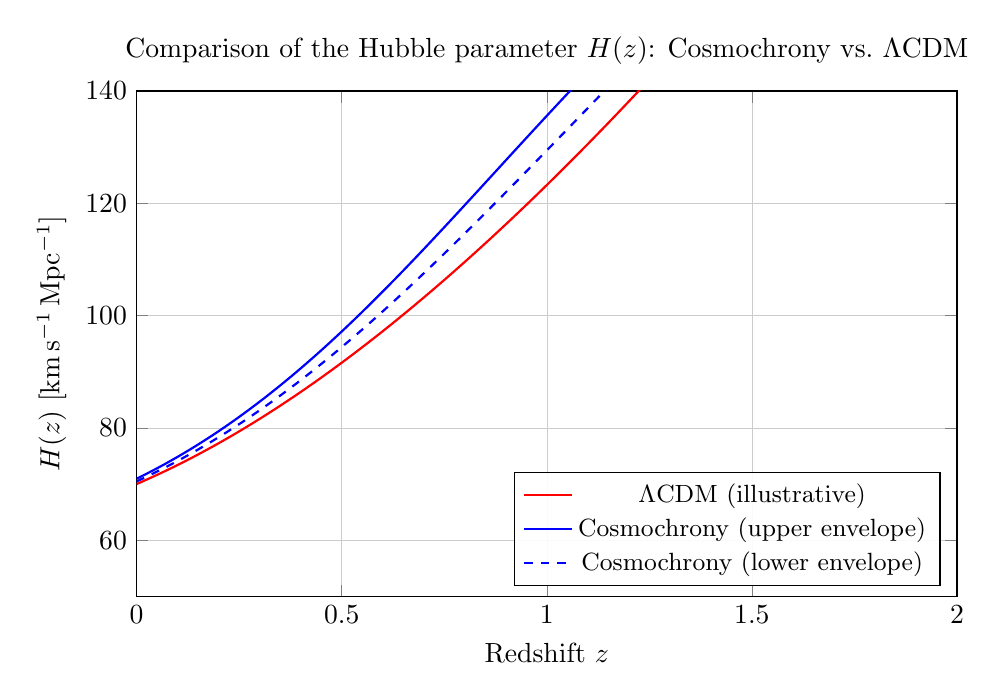
\begin{tikzpicture}
        \begin{axis}[
          width=12cm,
          height=8cm,
          title={Comparison of the Hubble parameter $H(z)$: Cosmochrony vs.\ $\Lambda$CDM},
        xlabel={Redshift $z$},
        ylabel={$H(z)$ [km\,s$^{-1}$\,Mpc$^{-1}$]},
        xmin=0, xmax=2,
        ymin=50, ymax=140,
        xtick={0,0.5,1,1.5,2},
        legend style={
          at={(rel axis cs:0.98,0.02)},
          anchor=south east,
          draw=black,
          fill=white,
          fill opacity=0.9,
          text opacity=1,
          font=\small
        },
        grid=both,
        grid style={line width=.1pt, draw=gray!10},
        major grid style={line width=.2pt, draw=gray!40},
        ]

          % --- Baseline LCDM ---
          \addplot[
            domain=0:2, samples=200,
            red, thick, mark=none
          ]
          {70*sqrt(0.3*(1+x)^3 + 0.7)};
          \addlegendentry{$\Lambda$CDM (illustrative)}

          % --- Cosmochrony band ---
          \addplot[
            domain=0:2, samples=200,
            blue, thick, mark=none
          ]
          {70*sqrt(0.3*(1+x)^3 + 0.7) * (1 + 0.10*exp(-2*(x-1)^2))};
          \addlegendentry{Cosmochrony (upper envelope)}

          \addplot[
            domain=0:2, samples=200,
            blue, thick, dashed, mark=none
          ]
          {70*sqrt(0.3*(1+x)^3 + 0.7) * (1 + 0.05*exp(-2*(x-1)^2))};
          \addlegendentry{Cosmochrony (lower envelope)}
        \end{axis}
      \end{tikzpicture}
      \caption{Schematic comparison of $H(z)$ in Cosmochrony and $\Lambda$CDM.
      Cosmochrony predicts a mild enhancement at intermediate redshifts due to
      relaxation inhomogeneities, providing a discriminating observational test.}
      \label{fig:hubble-comparison}
    \end{figure}

  \subsection{Redshift Drift}
  \label{subsec:redshift-drift}

  An implication of the monotonic relaxation dynamics developed in
  Section~\ref{subsec:expansion-as-relaxation} is that cosmological
  redshifts exhibit a slow temporal evolution when described in an effective
  spacetime parametrization.
  This leads to a redshift drift whose magnitude and redshift dependence differ
  quantitatively from those predicted by the standard $\Lambda$CDM model,
  particularly at intermediate redshifts.

  At the level of an effective parametrization, intended only as an order-of-magnitude
  estimate rather than a derived dynamical law, the effective drift rate may be
  written as
  \begin{equation}
    \dot{z}_{\mathrm{eff}}
    \;\sim\;
    H_0 (1+z) - \frac{c}{\chi(t)},
  \end{equation}
  where the second term reflects the ongoing relaxation of the $\chi$ substrate rather
  than a dark-energy-driven acceleration.
  This corresponds to a secular variation of order
  \[
    \Delta z \sim 10^{-10}\,\mathrm{yr}^{-1}
  \]
  at redshift $z \sim 1$, differing from $\Lambda$CDM expectations at the
  $\sim 10\%$ level in this regime.

  Future high-precision spectroscopic facilities, such as extremely large telescopes
  equipped with ultra-stable spectrographs, may be capable of probing this effect.
  A detection of a redshift drift incompatible with $\Lambda$CDM predictions would
  therefore provide a direct observational discriminator between geometric
  relaxation of the $\chi$ substrate and dark-energy-driven cosmic acceleration.

  \subsection{Gravitational Wave Propagation}
  \label{subsec:gravitational-wave-propagation}

  In the Cosmochrony framework, gravitational waves correspond to propagating
  collective modulations of the $\chi$ field in regimes where a spacetime
  description is applicable.
  They do not constitute independent propagating degrees of freedom, but reflect
  time-dependent redistributions of relaxation constraints within the field.

  In regions of high excitation density, such as near compact objects, the local
  slowdown of $\chi$ relaxation is expected to modify the propagation of these
  modulations.
  In particular, partial decoherence or attenuation may arise due to the coupling
  of propagating modulations to strongly constrained relaxation regions.
  These effects originate from the same collective relaxation constraints
  responsible for gravitational time dilation and horizon formation, and do not
  require the introduction of additional dynamical fields.

  \paragraph{Order-of-magnitude attenuation estimate.}
    Consider a compact object of mass $M$, characterized in effective geometric
    descriptions by a Schwarzschild radius
    \[
      r_s = \frac{2GM}{c^2}.
    \]
    Gravitational-wave modulations of the $\chi$ field propagating through regions
    where the effective relaxation rate is significantly reduced are expected to lose
    coherence through partial redistribution into non-propagating relaxation modes.

    For waves traversing regions within a characteristic distance
    \[
      r \lesssim 10\,\frac{GM}{c^2},
    \]
    the cumulative reduction of effective relaxation conductivity suggests an
    attenuation factor that may be parametrized, at the level of order-of-magnitude
    estimates, as
    \[
      \frac{\Delta A}{A} \sim \mathcal{O}(10^{-2} - 10^{-1}),
    \]
    where the precise magnitude depends on the local $\chi$ correlation length $\xi$
    and on the effective relaxation fraction $\Omega_\chi$ in the vicinity of the
    source.
    This attenuation should be interpreted as a redistribution of wave coherence
    within the $\chi$ relaxation dynamics rather than as dissipative energy loss in
    the conventional field-theoretic sense.

  \paragraph{Observational signature.}
    Such effects are expected to manifest most clearly during the late-time ringdown
    phase of binary black hole mergers, where gravitational-wave signals probe the
    strongly constrained relaxation regime near the effective horizon.
    The resulting signature would appear as a frequency-dependent deviation from
    general relativistic ringdown templates, potentially mimicking anomalous damping
    or mode-dependent quality factors.

    While current ground-based detectors do not yet achieve the signal-to-noise ratios
    required to resolve attenuation at the few-percent level, future space-based
    observatories operating in the LISA band, with expected signal-to-noise ratios
    exceeding $\sim 100$ for massive black hole mergers, may provide sufficient
    sensitivity to test this prediction.

  \paragraph{Semi-quantitative scaling estimate.}
    Within the Cosmochrony framework, attenuation of gravitational-wave amplitudes
    near compact objects arises from the local suppression of $\chi$ relaxation in
    regions of high effective curvature.
    At leading order, the relative amplitude reduction is expected to scale with the
    dimensionless curvature parameter $(r_s / r)$.

    A simple dimensional estimate yields
    \[
      \frac{\Delta A}{A} \sim \left( \frac{r_s}{r} \right)^2 ,
    \]
    indicating that the effect depends explicitly on both the compact object mass and
    the wave trajectory’s impact parameter.
    For propagation at distances $r \approx 10\,r_s$, this scaling gives
    \[
      \frac{\Delta A}{A} \sim 10^{-2},
    \]
    consistent with the order-of-magnitude estimates above and with exploratory
    numerical results obtained from $\chi$-field simulations
    (Appendix~D.3).

  \subsection{Galaxy Rotation Curves from Structural Relaxation}
  \label{subsec:galaxy-rotation-chi}

  As shown in Section~\ref{subsec:phi-eff-galaxies}, the Cosmochrony framework
  predicts modifications of galactic rotation curves arising from the structural
  relaxation of the projected \(\chi_{\mathrm{eff}}\) field, without introducing
  additional dark matter components.

  The Cosmochrony framework predicts modifications of galactic rotation curves arising
  from the structural relaxation of the projected \(\chi_{\mathrm{eff}}\) field, without
  introducing additional dark matter components.

  In regions where localized matter configurations induce persistent relaxation
  gradients in the \(\chi\)-substrate, the effective inertial response of orbiting matter
  is modified.
  This leads to an enhancement of tangential velocities at large radii, producing
  approximately flat rotation curves.

  Unlike modified gravity scenarios, this effect does not require an explicit change of
  the gravitational force law.
  It arises from a non-local redistribution of relaxation capacity in the projected
  description, tied to the large-scale coherence of the underlying \(\chi\)-configuration.

  Observable consequences include:
  \begin{itemize}
    \item a correlation between rotation curve flattening and indicators of structural
    relaxation activity rather than baryonic mass alone,
    \item deviations from simple baryonic scaling relations in dynamically young or
    disturbed galaxies,
    \item a reduced need for fine-tuned dark matter profiles in low-surface-brightness
    systems.
  \end{itemize}

  These signatures provide a discriminant between Cosmochrony, particle dark matter
  models, and purely phenomenological modified gravity approaches.

  \subsection{Spin and Topological Signatures}
  \label{subsec:spin-and-topological-signatures}

  An implication of the topological origin of spin developed in
  Section~\ref{subsec:spin_topology} is that, if particle spin originates from
  topologically nontrivial configurations of the $\chi$ substrate, then spin-related
  phenomena may admit geometric signatures not captured by purely algebraic quantum
  descriptions.

  In particular, ultra-high-precision interference experiments sensitive to
  $4\pi$ rotational symmetry may, in principle, probe deviations associated with
  the internal topology of localized projectable $\chi$ configurations.
  Such deviations would not modify standard spin--statistics relations, but could
  appear as extremely small phase shifts or coherence effects under closed
  $2\pi$ versus $4\pi$ rotational cycles.

  These signatures are expected to be strongly suppressed and therefore lie beyond
  current experimental resolution.
  However, their existence would provide a conceptually distinctive test of the
  topological origin of spin proposed in Cosmochrony, as opposed to interpretations
  in which spin is treated as an abstract representation of spacetime symmetry
  groups.

  \input{14-predictions/06-absence-of-dark-energy-signatures}
  \subsection{CMB Polarization Signatures (Outlook)}
  \label{subsec:cmb-polarization-signatures}

  As discussed in Section~\ref{subsec:cmb}, residual large-scale projective correlations
  inherited from the pre-geometric relaxation of the $\chi$ substrate are expected to
  imprint scale-dependent signatures on the Cosmic Microwave Background (CMB).
  In Cosmochrony, these correlations arise from the bounded and irreversible relaxation
  of $\chi$, locally constrained by the invariant speed $c$, without invoking any
  superluminal stretching or inflationary phase.
  As a consequence, correlations at the largest angular scales are naturally suppressed,
  leading to a reduction of power at low multipoles ($\ell \lesssim 10$).
  This mechanism is consistent with several large-angle features reported in CMB data,
  such as hemispherical asymmetry, without requiring fine-tuned initial conditions.
  Quantitative estimates of the resulting low-$\ell$ attenuation are discussed in
  Appendix~\ref{app:lowell_attenuation}.

  Observationally, the \emph{Planck} 2018 data report a suppression of the CMB quadrupole
  power at the level of $\sim 10\%$ relative to the $\Lambda$CDM best-fit expectation,
  corresponding to the long-standing low-$\ell$ anomaly at $\ell = 2$~\cite{Aghanim2020}.
  Within Cosmochrony, this suppression arises naturally from the pre-geometric relaxation
  dynamics of the $\chi$ substrate, which reduces large-angle correlations prior to the
  emergence of an effective spacetime description.
  Unlike phenomenological explanations relying on specific initial conditions or
  model-dependent modifications of primordial spectra, the effect follows directly from
  the intrinsic relaxation properties of the underlying field.

  \paragraph{Cosmological Imprints: The \texorpdfstring{$8/3$}{8/3} Scaling in CMB Polarization}
    \label{subsec:cmb_8_3_scaling}

    Beyond temperature anisotropies, the fundamental spectral ratio
    $\lambda_2/\lambda_1 = 8/3$, which governs the electroweak mass hierarchy at the
    micro-scale (see Appendix~\ref{sec:spectral_ratio_derivation}), is expected to leave a
    structural signature in the polarization sector of the CMB.
    In this framework, primordial scalar and tensor perturbations are reinterpreted as
    dual manifestations of the substrate's relaxation, corresponding respectively to
    base transmittance and fiber shear modes of the projection.

    \subparagraph{Geometric Bound on the Tensor-to-Scalar Ratio (\texorpdfstring{$r$}{r})}

      In Cosmochrony, the tensor-to-scalar ratio $r$ is constrained by the relative spectral
      stiffness of the $\chi$ substrate's projection modes.
      Under the principle of \textbf{Projective Spectral Saturation} at the high-energy limit
      ($k \approx 1/h_\chi$), the relaxation energy $\mathcal{E}$ is distributed according to
      the maximal kinematic capacity of each mode:
    \begin{equation}
      \mathcal{E}_s \propto \lambda_{\text{base}} \Delta_s^2,
      \qquad
      \mathcal{E}_t \propto \lambda_{\text{fiber}} \Delta_t^2 .
      \end{equation}
      The ``bare'' geometric ratio $r_0$ is defined by the saturation of these spectral densities:
    \begin{equation}
      r_0
      = \frac{\Delta_t^2}{\Delta_s^2}
      = \frac{\lambda_{\text{base}}}{\lambda_{\text{fiber}}}
      = \frac{3}{8}
      \simeq 0.375 .
      \end{equation}
      This value does not correspond to an observable tensor-to-scalar ratio at recombination,
      but defines a \emph{geometric upper bound} imposed by the topology of the projection fiber
      at the saturation scale.

    \subparagraph{Topological Decoherence and Parametrization of \texorpdfstring{$r_{\text{obs}}$}{robs}}

      The observed ratio $r_{\text{obs}}$ undergoes \textbf{topological decoherence} as the
      substrate expands.
      Since fiber shear modes are intrinsically more sensitive to losses of projective
      alignment, the cumulative degradation of alignment induces a monotonic suppression
      of tensor modes.
      To leading order, this effect may be effectively parametrized as
    \begin{equation}
      r_{\text{obs}}(t)
      = r_0 \cdot \exp\!\left( -\zeta \frac{\tau_\chi}{t} \right),
      \end{equation}
      where $\tau_\chi$ denotes the characteristic relaxation time of the substrate.
      The precise functional form is not fundamental and merely encodes the fact that fiber
      shear modes decohere faster than base transmittance during cosmic relaxation.
      This decay represents the transition from the primordial saturated state to the
      present large-scale geometric stability, providing a structural explanation for the
      low observed value of $r$ ($r < 0.036$), without invoking slow-roll dynamics or
      fine-tuned inflationary potentials.

  \subsection{Neutrino-Mediated Relaxation and Decay Signatures}
  \label{subsec:neutrino-decay-signatures}

  An implication of the structural interpretation of particle decay
  (Section~\ref{subsec:metastability-and-decay}) together with
  the partial projectability of neutrino modes
  (Section~\ref{subsec:neutrinos-partially-projectable-modes}) is that, in
  Cosmochrony, particle decay and neutrino emission are manifestations of structural
  reorganization rather than independent microscopic processes.
  This interpretation leads to distinct observational signatures.

  Because neutrino-like excitations act as non-local relaxation channels, decay processes
  in the early universe contribute to an irreversible smoothing of admissible configurations.
  This smoothing is expected to leave detectable imprints across multiple observational domains.

  Specifically, the framework predicts:
  \begin{itemize}
    \item an enhanced role of neutrino backgrounds in suppressing large-scale coherence
    without behaving as conventional radiation pressure,
    \item a weak coupling between decay rates and late-time environmental conditions,
    reflecting their origin in early structural metastability,
    \item possible correlations between decay-driven neutrino emission and large-scale
    anisotropies observed in the cosmic microwave background.
  \end{itemize}

  At the particle-physics level, this interpretation suggests that decay lifetimes and
  branching ratios encode information about the stability landscape of admissible
  projected configurations rather than fundamental stochasticity.
  Future precision measurements of rare decays may therefore provide indirect probes of
  the structural relaxation dynamics underlying the Cosmochrony framework.

  \subsubsection*{Environmental Modulation of Particle Stability}
    \label{subsec:environmental-decay-modulation}

    A distinctive prediction of the Cosmochrony framework is that particle stability is not
    strictly universal, but may exhibit a weak dependence on the surrounding structural environment.
    Because particle decay originates from the susceptibility of metastable projected
    configurations to their own admissible fluctuations, any factor that modifies the local
    relaxation landscape can, in principle, affect decay rates.

    In regions characterized by strong gradients of the \(\chi\) substrate—such as galactic
    cores or highly structured gravitational environments—the spectrum and amplitude of
    admissible fluctuations are expected to differ slightly from those in weakly structured
    regions.
    As a result, the effective lifetime of unstable particles may acquire a small environment-dependent modulation.

    This effect is predicted to be extremely weak and therefore compatible with all current
    laboratory and astrophysical constraints.
    Nevertheless, it represents a qualitatively new signature: a violation of strict
    universality of decay rates induced not by local interactions or spacetime curvature,
    but by structural relaxation gradients in the underlying relational substrate.

    Future high-precision measurements of decay processes in environments with strong
    gravitational or structural gradients, as well as dedicated numerical simulations of
    \(\chi\)-field dynamics, may allow quantitative estimates of this effect.
    Its detection or exclusion would provide a direct and stringent test of the Cosmochrony framework.

    \paragraph{Order-of-magnitude estimate.}

      Within the Cosmochrony framework, the effective lifetime of an unstable particle is
      controlled by the susceptibility of a metastable projected configuration to its own
      admissible fluctuations.
      Because the spectrum and density of such fluctuations depend weakly on the surrounding
      structural environment, a small modulation of decay rates is expected in regions
      characterized by strong gradients of the \(\chi\) substrate.

      A minimal parametrization of this effect may be written as
    \begin{equation}
      \frac{\delta \Gamma}{\Gamma}
      \;\simeq\;
      \beta\,\frac{\Delta U}{c^2},
      \end{equation}
      where \(\Gamma\) is the decay rate, \(U\) denotes an effective gravitational or
      structural potential serving as a proxy for the local relaxation gradient, and
      \(\beta\) is a dimensionless sensitivity coefficient encoding the response of the
      projected configuration to environmental variations.

      Existing tests of local position invariance based on high-precision atomic clocks
      strongly constrain any environmental dependence of effective physical rates.
      Requiring compatibility with these constraints suggests a conservative bound
      \(\beta \lesssim 10^{-6}\).

      For typical galactic environments, the difference in effective potential between
      weakly structured regions and galactic cores is of order
      \(\Delta U / c^2 \sim 10^{-7}\)–\(10^{-6}\).
      Combining these estimates yields a fractional modulation of particle lifetimes of
      order
    \begin{equation}
      \frac{\delta \tau}{\tau}
      \;\sim\;
      10^{-13}\text{--}10^{-12}.
      \end{equation}

      Such an effect is far below the sensitivity of current laboratory measurements and
      therefore fully compatible with existing experimental bounds.
      Nevertheless, it represents a qualitatively novel signature: a weak violation of the
      strict universality of decay rates induced not by spacetime curvature or local
      interactions, but by structural relaxation gradients in the underlying relational
      substrate.
      Future high-precision astrophysical observations or dedicated numerical simulations of
      \(\chi\)-field dynamics may allow this prediction to be further quantified or
      constrained.

    \paragraph{Which decay channels are most sensitive?}

      In Cosmochrony, an environmental modulation of decay rates is expected to be largest
      for metastable configurations whose admissible fluctuation spectrum is only weakly
      protected by topology, and whose decay proceeds through a comparatively ``thin''
      projective channel (small number of admissible final factorizable branches).
      This suggests the following qualitative hierarchy of experimental leverage:

    \begin{itemize}
      \item \textbf{Purely leptonic weak decays} (e.g.\ \(\mu^\pm \to e^\pm \nu \bar{\nu}\)):
      theoretically clean (minimal hadronic uncertainty), with extremely well-characterized
      kinematics. The limitation is practical: \(\tau_\mu\) is measured very precisely, but
      changing the \emph{structural environment} sufficiently in the laboratory is difficult.

      \item \textbf{Hadronic weak decays and oscillating neutral mesons}
      (e.g.\ \(K^0\)--\(\bar{K}^0\), \(B^0\)--\(\bar{B}^0\)):
      in standard physics these are exquisitely sensitive to tiny perturbations in the
      effective Hamiltonian. In Cosmochrony terms, they probe whether the projection fiber
      admits a detectable environment-dependent bias between conjugate branches.
      The price is interpretability: hadronic and medium effects require careful control.

      \item \textbf{Nuclear \(\beta\)-decays and long-lived isotopes}:
      exceptionally good metrological stability allows long integration times, but nuclear
      structure systematics are harder to disentangle from any putative projective effect.

      \end{itemize}

      Overall, the cleanest conceptual target is leptonic weak decay, while the most
      ``amplified'' interferometric target is neutral-meson mixing, provided that standard
      environmental systematics are tightly controlled.

    \paragraph{Differential astrophysical signature.}

      Directly comparing lifetimes of unstable particles between ``void'' and typical
      galactic cores is observationally challenging, because decay processes are not
      tagged \emph{in situ}.
      However, Cosmochrony predicts a \emph{differential} effect that can in principle be
      searched for in environments where the effective potential proxy \(\Delta U/c^2\)
      is substantially larger than in ordinary galactic regions.

      In particular, energetic hadronic cascades near compact objects (accretion flows and
      relativistic jets) are controlled by the competition between interaction lengths and
      decay lengths of \(\pi^\pm\), \(K^\pm\), and \(\mu^\pm\), which shapes the emergent
      high-energy \(\gamma\)-ray and neutrino spectra.
      If decay rates acquire a weak environmental modulation,
    \begin{equation}
      \frac{\delta \Gamma}{\Gamma} \simeq \beta\,\frac{\Delta U}{c^2},
      \end{equation}
      then the \emph{effective} critical energy at which decay dominates over interaction
      is shifted by the same fractional amount,
    \begin{equation}
      \frac{\delta E_\ast}{E_\ast} \sim \frac{\delta \tau}{\tau}
      \sim \beta\,\frac{\Delta U}{c^2}.
      \end{equation}

      Near the innermost regions of accretion flows around massive compact objects,
      a characteristic scale \(\Delta U/c^2 \sim 10^{-4}\) is not excluded as an order-of-magnitude proxy,
      leading (for conservative \(\beta \lesssim 10^{-6}\)) to
    \begin{equation}
      \frac{\delta \tau}{\tau} \sim 10^{-10},
      \end{equation}
      still extremely small, but conceptually clean: a systematic, environment-correlated
      spectral bias that cannot be mimicked by late-time cosmological parameter shifts.

      The key discriminant is \emph{correlation with environment}:
      sources with otherwise similar intrinsic properties but different compactness proxies
      (e.g.\ inferred emission radius or gravitational redshift indicators) should exhibit
      a tiny but coherent shift in the decay-limited spectral features of hadronic secondaries.

    \paragraph{Connection to numerical \(\chi\)-field simulations.}

      The sensitivity coefficient \(\beta\) can be operationally defined and extracted from
      \(\chi\)-field simulations by measuring how the \emph{escape time} of a metastable
      localized configuration changes when embedded in a controlled background gradient.

      Let \(\tau_0\) denote the mean first-passage (escape) time of a metastable localized
      configuration in a reference background, estimated from an ensemble of runs with
      different admissible fluctuation seeds.
      Introduce a dimensionless structural gradient proxy \(G\) (computed from the projected
      field) such as
    \begin{equation}
      G \;\equiv\; \frac{\ell^2}{\chi_0^2}\,\langle |\nabla \chi_{\mathrm{eff}}|^2 \rangle_{\mathcal{R}},
      \end{equation}
      where \(\ell\) is a chosen coarse-graining scale, \(\chi_0\) a normalization, and
      \(\langle \cdot \rangle_{\mathcal{R}}\) denotes averaging over a region \(\mathcal{R}\)
      containing the localized excitation.

      Define the empirical susceptibility
    \begin{equation}
      S \;\equiv\; \frac{d\ln \tau}{dG},
      \end{equation}
      estimated numerically by repeating the experiment at slightly different controlled
      background gradients \(G\).
      A minimal mapping to the phenomenological parametrization
      \(\delta\tau/\tau \simeq \beta\,\Delta U/c^2\) is then obtained by specifying an
      effective correspondence between \(\Delta U/c^2\) and \(\Delta G\) in the simulation,
    \begin{equation}
      \frac{\delta \tau}{\tau} \;\simeq\; S\,\Delta G
      \;\equiv\; \beta\,\frac{\Delta U}{c^2}.
      \end{equation}

      In practice, this provides a clear numerical pipeline:
      (i) prepare a metastable localized configuration, (ii) embed it in backgrounds with
      controlled \(G\), (iii) estimate \(\tau(G)\) from ensembles, and (iv) infer \(S\),
      hence \(\beta\), up to the chosen environment proxy mapping.
      The resulting \(\beta\) can then be confronted with the conservative metrological
      requirement \(\beta \lesssim 10^{-6}\).

  \subsection{Environmental Modulation of Particle Lifetimes}
  \label{subsec:environmental-modulation-lifetimes}

  Within the Cosmochrony framework, particle decay is not interpreted as a
  fundamental stochastic process, but as the manifestation of the
  \emph{structural susceptibility} of a metastable projected configuration
  to admissible fluctuations of the underlying relational substrate $\chi$.
  As discussed in Section~\ref{subsec:neutrino-decay-signatures}, these
  fluctuations form a bounded background whose spectral density depends
  weakly on the local relaxation structure of $\chi$.

  As a consequence, the decay rate $\Gamma$ of an unstable particle is not
  strictly universal, but may exhibit an extremely small environmental
  dependence reflecting variations in the local relaxation gradient of the substrate.
  At leading order, this effect may be parametrized as
  \begin{equation}
    \frac{\delta \Gamma}{\Gamma}
    \;\simeq\;
    \beta \, \frac{\Delta U}{c^{2}},
    \label{eq:lifetime-modulation}
  \end{equation}
  where $U$ denotes an effective gravitational or structural potential
  serving as a proxy for the local relaxation density, and $\beta$ is a
  dimensionless sensitivity parameter encoding the coupling between the
  projected metastable configuration and the admissible substrate fluctuations.

  Since the particle lifetime is given by $\tau = \Gamma^{-1}$, the relative
  variation of the lifetime satisfies, to first order,
  \begin{equation}
    \frac{\delta \tau}{\tau}
    \;\simeq\;
    - \frac{\delta \Gamma}{\Gamma}.
  \end{equation}

  Existing experimental constraints on local position invariance, in
  particular those derived from high-precision atomic clock comparisons,
  suggest a conservative upper bound $\beta \lesssim 10^{-6}$.
  Typical contrasts in effective potential between weakly structured
  environments and regions of high structural density (e.g.\ galactic
  cores) correspond to $\Delta U / c^{2} \sim 10^{-7}$--$10^{-6}$.
  Under these conditions, Cosmochrony predicts
  \begin{equation}
    \frac{\delta \tau}{\tau}
    \;\sim\;
    10^{-13} \text{--} 10^{-12},
    \label{eq:lifetime-order-of-magnitude}
  \end{equation}
  well below current laboratory sensitivities, but conceptually distinct
  from standard quantum or relativistic effects.

  Importantly, this modulation does not arise from spacetime curvature,
  local interactions, or environmental decoherence, but from the structural
  properties of the non-injective projection from $\chi$ to its effective
  description.
  A future detection of even a minute, reproducible deviation from strict lifetime universality would therefore
  constitute a direct signature of the underlying relational substrate.

  \subsection{Summary}
  \label{subsec:summary6}

  Within the Cosmochrony framework, gravity does not arise as a fundamental interaction
  or as an independent geometric degree of freedom.
  It emerges at the level of effective descriptions as a macroscopic consequence of
  localized projected configurations collectively constraining admissible relaxation
  ordering.

  Classical gravitational phenomena—including gravitational time dilation, effective
  spacetime curvature, gravitational waves, and black holes—are recovered as distinct
  descriptive regimes of this collective constraint.
  They reflect variations in the projectability and correlation structure of admissible
  descriptions, rather than the dynamics of a fundamental spacetime or gravitational
  field.

  In this perspective, gravitation appears as an emergent, operational phenomenon,
  summarizing how localized projected configurations collectively limit admissible
  ordering and correlation across extended regions, without introducing gravity as a
  primitive force or fundamental geometric entity.


  \section{Discussion and Comparison with Existing Frameworks}
  \label{sec:discussion-and-comparison-with-existing-frameworks}

  The Cosmochrony framework proposes a minimal pre-geometric substrate, described by
  a single scalar quantity $\chi$, whose irreversible relaxation underlies both
  microscopic and cosmological phenomena.
  Spacetime geometry, gravitational dynamics, and quantum behavior arise only as
  effective descriptions of this underlying relaxation process.

  In this section, we discuss how this approach relates to established theoretical
  frameworks, highlight its conceptual implications, and identify open challenges.
  Particular emphasis is placed on clarifying points of contact and distinction with
  general relativity, quantum mechanics, and standard cosmological models, as well as
  on assessing the ontological and methodological economy of the framework.

  The goal is not to claim empirical superiority over existing theories, but to
  clarify the conceptual role of Cosmochrony as a deeper explanatory layer from which
  standard frameworks emerge in appropriate regimes.

  \subsection{Relation to General Relativity}
  \label{subsec:relation-to-general-relativity}

  General Relativity (GR) describes gravitation as the curvature of spacetime induced
  by energy--momentum.
  In Cosmochrony, no \emph{a priori} metric dynamics is postulated at the fundamental
  level.
  Instead, an effective spacetime geometry emerges as a descriptive framework from
  variations in the local relaxation dynamics of the $\chi$ field.

  Matter configurations, modeled as stable or metastable topological excitations of
  $\chi$, locally constrain the relaxation of the field.
  This leads to differential rates of effective proper-time evolution between
  neighboring regions.
  When expressed in geometric terms, these differences can be reinterpreted as an
  effective deformation of the spacetime metric.

  In the weak-field regime, this mechanism reproduces Newtonian gravity, while in the
  strong-field limit it yields Schwarzschild-like solutions in effective geometric
  descriptions.
  The resulting phenomenology is therefore consistent with the empirical successes
  of GR across its tested domain.

  From this perspective, gravitation is not introduced as a fundamental interaction,
  but emerges as a macroscopic manifestation of inhomogeneous $\chi$ relaxation.
  General Relativity is recovered as the appropriate effective theory describing
  this regime, rather than being supplanted or modified at the level of observable
  predictions.

  \subsection{Relation to Quantum Formalism}
  \label{subsec:relation-to-quantum-formalism}

  Quantum mechanics and quantum field theory (QFT) introduce probabilistic
  wavefunctions, operators, and quantization rules as foundational postulates~\cite{PeskinSchroeder1995QFT}.
  In contrast, Cosmochrony does not treat quantization or wave dynamics as fundamental.
  Instead, it describes a continuous pre-geometric relational substrate whose
  projected and thresholded effective descriptions give rise to the formal apparatus of quantum theory.

  Within this framework, particles correspond to localized, topologically stable configurations of the $\chi$ substrate.
  Discrete observables arise not from intrinsic microscopic discreteness, but from
  boundary conditions, topological constraints, and interaction-induced
  reprojection, which select a finite set of stable effective configurations.

  The Planck relation $E = h\nu$ is interpreted geometrically as a correspondence
  between the amount of relaxation potential redistributed during an interaction
  and the minimal projective resolution required for a coherent effective spacetime description.
  The parameter $\nu$ does not represent a fundamental oscillation of $\chi$, but a
  frequency characterizing the projective structure of the emergent spacetime description.

  Quantum correlations are described in purely relational terms.
  Entanglement corresponds to the persistence of a shared, non-factorizable $\chi$
  configuration across spatial separation, while decoherence reflects the
  irreversible loss of relational accessibility due to interaction with the environment.
  This interpretation reproduces standard quantum phenomenology, including
  nonlocal correlations, without invoking superluminal signaling, fundamental
  wavefunction collapse, or hidden variables.

  Importantly, within Cosmochrony such non-factorizable correlations are not generic:
  they persist only within a finite, critical regime of projection, and are suppressed
  when spectral rigidity, environmental coupling, or effective mass drive projected
  descriptions toward over-compression and effective factorization.

  \subsection{Analogy with Collective Phenomena in QCD}
  \label{subsec:analogy-with-collective-phenomena-in-qcd}

  A useful structural analogy may be drawn with quantum chromodynamics (QCD) in the
  low-energy regime, where the fundamental degrees of freedom introduced in the
  theory do not correspond directly to observable particles~\cite{Shifman2007QCDVacuum}.
  Quarks and gluons are not detected as isolated entities in spacetime; instead,
  hadronic properties, effective masses, and confinement phenomena emerge from a
  strongly interacting collective vacuum structure.

  In a similar conceptual spirit, the Cosmochrony framework does not attribute
  gravitational or quantum phenomena to fundamental fields propagating on a
  pre-existing spacetime.
  At the fundamental level, the theory is formulated solely in terms of the
  pre-geometric relational substrate $\chi$ and its intrinsic relaxation dynamics.
  Observable physical quantities arise only after projection, in regimes where
  $\chi$ admits a stable and sufficiently smooth effective description.

  In such regimes, it is convenient to introduce effective quantities, collectively
  denoted $\chi_{\mathrm{eff}}$, which summarize coarse-grained, relationally stable
  features of the underlying $\chi$ configurations.
  These effective quantities are not additional ontological layers, nor independent
  degrees of freedom.
  They function as regime-dependent descriptors, encoding how the relational
  structure of $\chi$ becomes expressible in terms of fields, observables, and
  geometric notions within emergent spacetime.

  This hierarchy of descriptions closely parallels the situation in QCD.
  While quarks constitute indispensable degrees of freedom at the level of the
  microscopic theory, their physical relevance is restricted to specific regimes,
  and they do not appear as freely propagating particles in the asymptotic spectrum.
  Their absence from direct observability does not signal incompleteness, but
  reflects the collective and confined nature of the underlying dynamics.

  Likewise, Cosmochrony does not require that all internal structures invoked in its
  description correspond to independently observable entities.
  What appear as elementary constituents at a given effective level may instead
  represent stable, regime-dependent invariants of the underlying $\chi$ dynamics.
  The absence of direct observability of such structures is therefore not a defect of
  the framework, but a natural consequence of its pre-geometric and relational
  character.

  As in QCD, the appropriate physical description in Cosmochrony depends critically
  on the scale and regime considered.
  While the fundamental dynamics of $\chi$ are simple in principle, the emergent
  macroscopic behavior is governed by nonlinear and collective effects that are most
  naturally captured by effective and phenomenological descriptions.
  This reinforces the view that geometry, gravitation, and quantum observables in
  Cosmochrony are emergent constructs, rather than fundamental ontological
  primitives.

  \subsection{Comparison with $\Lambda$CDM Cosmology}
  \label{subsec:comparison-with-lambdacdm-cosmology}

  The $\Lambda$CDM model provides a remarkably successful phenomenological
  description of large-scale cosmological observations by introducing cold dark
  matter, dark energy, and an early inflationary phase~\cite{peebles1993principles,planck2020results}.
  However, these components are postulated at the level of the effective model and
  are not derived from more fundamental principles.

  In Cosmochrony, cosmic expansion follows directly from the monotonic relaxation
  of the fundamental substrate $\chi$.
  The observed Hubble law emerges as a kinematic consequence of differential
  relaxation, without invoking a cosmological constant.
  When expressed in an effective geometric description, the expansion rate may be
  written as
  \begin{equation}
    H(t) = \frac{\dot{\chi}}{\chi},
  \end{equation}
  leading naturally to $H_0 \sim c / \chi(t_0)$ in the late-time regime.

  From this perspective, dark energy is not interpreted as an additional physical
  component, but as an effective description of the large-scale relaxation
  dynamics of $\chi$.
  Cosmic acceleration reflects the cumulative manifestation of this process over
  cosmological timescales.
  At the homogeneous and isotropic level, Cosmochrony reproduces the background
  expansion described by Friedmann--Lema\^{\i}tre cosmology, while offering an
  alternative interpretation of its underlying physical origin.

  Unlike $\Lambda$CDM, which introduces empirically fitted initial conditions
  and a persistent dark energy component, the Cosmochrony framework attributes the
  late-time acceleration to the intrinsic relaxation properties of the underlying
  field.
  In this view, the coincidence problem and the observed tension between local and
  global measurements of the Hubble parameter may admit an interpretation in terms of epoch-dependent relaxation
  dynamics rather than as indications of new fundamental constituents.

  At large angular scales, $\Lambda$CDM treats deviations from scale invariance in
  the cosmic microwave background (CMB) as statistical realizations around an
  ensemble-averaged spectrum, with individual low-$\ell$ modes subject to cosmic
  variance.
  Within Cosmochrony, constraints on the largest-scale configurations of the
  $\chi$ field allow for a scale-dependent attenuation of global modes.
  From this standpoint, the observed suppression of power at low multipoles may be
  may be explored as a possible structural consequence of the relaxation dynamics, rather than
  as a purely statistical fluctuation.

  Taken together, these considerations suggest that Cosmochrony offers an
  alternative interpretative framework for cosmological observations, while
  remaining compatible with the empirical successes of the standard model at the
  level of current observational precision.

  \subsection{Inflation, Horizon Problems, and Initial Conditions}
  \label{subsec:inflation-horizon-problems-and-initial-conditions}

  Standard inflationary theory addresses the horizon, flatness, and monopole
  problems by postulating a brief phase of accelerated expansion driven by an
  inflaton field.
  In the Cosmochrony framework, these issues are approached from a different
  conceptual standpoint.

  Because the fundamental field $\chi$ defines a global relaxation process rather
  than a metric expansion imposed externally, causal connectivity is preserved at
  the level of the underlying field dynamics.
  Large-scale coherence may therefore arise from the initial smoothness of $\chi$
  and its subsequent monotonic relaxation, potentially alleviating the need for a
  distinct inflationary epoch as a fundamental assumption.

  At this stage, this perspective should be regarded as an alternative
  interpretative framework rather than a complete replacement for inflationary
  cosmology.
  A detailed analysis of primordial perturbations, their spectrum, and their
  imprint on the cosmic microwave background (CMB) is required to determine the
  extent to which Cosmochrony reproduces, modifies, or departs from standard
  inflationary predictions.

  These questions define a clear direction for future work, in which the
  connection between early-time $\chi$ dynamics and observable cosmological
  signatures can be explored quantitatively.

  \subsection{Conceptual Implications and Open Challenges}
  \label{subsec:conceptual-implications-and-open-challenges}

  Cosmochrony proposes a unifying conceptual framework in which time, distance,
  energy, gravitation, and quantization emerge from the dynamics of a single
  pre-geometric relational substrate.
  This ontological economy constitutes a central strength of the framework, while
  also requiring a careful reassessment of notions traditionally treated as
  independent physical primitives.

  In particular, the framework suggests that time, energy, and irreversibility do
  not correspond to distinct fundamental entities.
  Temporal ordering arises from the monotonic relaxation of the $\chi$ substrate,
  while energy quantifies the residual capacity of localized configurations to
  resist this relaxation.
  Irreversibility then reflects the progressive exhaustion of such relaxation
  capacity.
  From this perspective, temporal flow and energetic processes are not independent
  axioms of nature, but complementary effective descriptions of the same underlying
  relational dynamics.

  At the level of effective physical descriptions, these relations are encoded in
  coarse-grained quantities such as $\chi_{\mathrm{eff}}$, which summarize how the
  relaxation structure of $\chi$ manifests in spacetime-based observables.
  These effective constructs carry no independent ontological status and remain
  valid only within regimes where a geometric interpretation is applicable.

  A concrete realization of this unification, including an explicit formulation of
  the relaxation operator and its spectral role in mass generation, is outlined in
  Appendix~\ref{subsec:perspectives_mass_spectrum}.
  While this reinterpretation addresses several long-standing conceptual tensions
  ---including the origin of the arrow of time and the status of energy conservation
  ---it also raises important open challenges.

  Among these challenges are:
  \begin{itemize}
    \item the quantitative reconstruction of cosmic microwave background anisotropies
    from early-time $\chi$ dynamics,
    \item the detailed treatment of non-equilibrium quantum measurements, decoherence,
    and reprojection processes,
    \item the emergence of gauge symmetries and interaction hierarchies from
    topological and relational features of $\chi$,
    \item and the long-term stability of solitonic particle configurations under
    extreme gravitational or radiative conditions.
  \end{itemize}

  Addressing these issues will require a combination of analytical, numerical, and
  experimental approaches, including:
  \begin{enumerate}
    \item large-scale numerical simulations of $\chi$ dynamics to quantify structure
    formation and cosmological signatures,
    \item the exploration of discretized, network-based, or lattice realizations of
    $\chi$ at microscopic scales,
    \item and targeted experimental tests of predicted $\chi$-dependent effects in
    quantum coherence, gravitation, and radiation processes.
  \end{enumerate}

  Progress along these directions may elevate Cosmochrony from a unifying
  interpretative framework to a quantitatively predictive theory, while preserving
  its minimal ontological foundation.

  \subsection{Ontological Parsimony and the Metric}
    \label{subsec:ontological-parsimony-and-the-metric}

    A potential criticism of Cosmochrony is that it merely replaces one geometric structure (the metric) with another
    (the $\chi$ field).
  This section addresses why this replacement constitutes genuine ontological progress rather than relabeling.

  \paragraph{Distinction from metric theories.}
    In General Relativity and its extensions:
    \begin{itemize}
      \item The metric $g_{\mu\nu}$ is a fundamental tensor field with 10 independent components.
      \item Spacetime curvature is a primitive geometric property.
      \item Matter and energy are conceptually distinct from geometry, coupled via the stress-energy tensor.
    \end{itemize}

    In Cosmochrony:
    \begin{itemize}
      \item Only the scalar field $\chi$ (1 component) is fundamental.
      \item The metric is a derived effective description, not an independent dynamical entity.
      \item Matter, energy, and geometry are unified as different manifestations of $\chi$ configurations.
    \end{itemize}

  \paragraph{Operational distinguishability.}
    The frameworks are operationally distinct:
    \begin{enumerate}
      \item \textbf{Degrees of freedom:} GR propagates 2 gravitational wave polarizations from 10 metric components.
      Cosmochrony propagates perturbations of 1 scalar field, with effective tensorial structure emerging only macroscopically.

      \item \textbf{Singularities:} GR singularities (where $g_{\mu\nu}$ diverges) are ontological.
      In Cosmochrony, apparent singularities mark the breakdown of the effective metric description, while $\chi$ remains well-defined.

      \item \textbf{Quantum regime:} Quantizing GR requires quantizing the metric (Wheeler-DeWitt equation).
      Quantizing Cosmochrony requires only quantizing $\chi$, with spacetime emerging from quantum $\chi$ configurations.
    \end{enumerate}

  \paragraph{The Occam's razor argument.}
    Cosmochrony achieves unification through reduction:
    \begin{align}
      \text{Traditional:} \quad & g_{\mu\nu} \,(\text{10 DOF}) + \psi \,(\text{matter}) + \Lambda \,(\text{dark energy}) \\
      \text{Cosmochrony:} \quad & \chi \,(\text{1 DOF}) \longrightarrow \{\text{spacetime}, \text{matter}, \text{expansion}\}
    \end{align}

    This represents genuine explanatory compression, not mere reformulation.

  \subsection{Relation to the Higgs Mechanism}
  \label{subsec:relation-to-the-higgs-mechanism}

  In the Standard Model, particle masses arise through spontaneous symmetry breaking of the electroweak sector, mediated
  by the Higgs field.
  In Cosmochrony, mass is not introduced as a fundamental parameter but emerges as a measure of resistance of localized
  $\chi$ configurations to the global relaxation flow.

  These two descriptions are not in contradiction.
  Rather, the Higgs field may be understood as an effective low-energy manifestation of the interaction between
  solitonic excitations and the surrounding $\chi$ background.
  In this view, the Higgs condensate encodes how localized field configurations acquire inertial properties within an
  already structured geometric substrate.

  Cosmochrony does not deny the empirical success of the Higgs mechanism, nor does it seek to modify its phenomenology
  at accessible energies.
  Instead, it suggests that the Higgs field is not fundamental, but emergent, much like the spacetime metric or quantum
  wavefunctions.
  The observed Higgs boson would then correspond to a collective excitation of the $\chi$ field associated with mass
  stabilization.
  In this framework, the Higgs vacuum expectation value (VEV) would be indirectly determined by
  the local properties of the $\chi$ background, effectively coupling the micro-physics of particle
  masses to the macro-dynamics of cosmic relaxation.

  A detailed derivation of the Higgs sector as an effective theory emerging from $\chi$ dynamics lies beyond the scope
  of the present work and is left for future investigation.


  \section{Conclusion and Outlook}
  \label{sec:conclusion-and-outlook}

  We have presented Cosmochrony, a minimalist framework in which a single fundamental entity, $\chi$, underlies the
  emergence of time, spacetime geometry, and a wide spectrum of physical phenomena.
  By identifying the irreversible relaxation of $\chi$ as the primary physical process, we have shown that familiar
  structures—from the metric tensor to the Standard Model—are not independent axioms but emergent harmonics of this relaxation.

  \textbf{A central result of this work is the \emph{ab initio} derivation of the dynamical laws.}
  Rather than postulating a convenient action, we have demonstrated that the Born--Infeld-like Lagrangian is the
  unique functional compatible with the causal saturation of relaxation fluxes at the speed $c_\chi$.
  By resolving the circularity between configuration and distance through spectral graph theory, we have
  established that spacetime geometry is the continuum encoding of microscopic connectivity, naturally recovering
  General Relativity as a thermodynamic limit.

  The framework provides a unified geometric origin for the Standard Model:
  \begin{itemize}
    \item \textbf{Gauge Interactions:}
    Reinterpreted as projection dynamics, where photons manifest as scalar transmittance and $W/Z$
    bosons as shear modes of the projection fiber, accounting for their mass without requiring a fundamental Higgs field
    as a primary ontological ingredient.
    \item \textbf{Matter and Mass:}
    Fermionic properties emerge from topological obstructions in the configuration space of $\chi$
    , while inertial mass is not postulated but arises from resistance to global relaxation, quantified by the
    \textit{spectral overlap} between localized excitations and the relaxation background.
    \item \textbf{The Dark Sector:}
    Within the same projection-based ontology, Dark Matter is identified as non-projected spectral density(sub-threshold
    inertia), contributing to gravitation without admitting a stable effective-field representation, while Dark Energy
    manifests as the global, irreversible relaxation flux $\Phi_\chi$.
  \end{itemize}

  At cosmological scales, expansion and the arrow of time follow directly from the diminishing tempo of relaxation as
  the substrate irreversibly approaches equilibrium.
  Within this framework, ``inflation'' and ``dark energy'' do not appear as fundamental ingredients, but as effective
  descriptions: their explanatory roles are replaced by pre-geometric connectivity in the early constrained regime and
  by epoch-dependent relaxation dynamics at late times.

  Beyond its conceptual unification, Cosmochrony offers a concrete program for validation.
  The transition from discrete relational constraints to effective field descriptions identifies clear numerical
  signatures for lattice simulations.
  While challenges remain—notably the precise numerical computation of the particle mass hierarchy—the framework now
  provides a complete, self-consistent theoretical bridge from the pre-geometric substrate to observable reality.

  By reducing the fundamental assumptions to a single dynamical origin, Cosmochrony offers a coherent foundation in
  which time, mass, and geometry arise as a unified whole.
  It provides a physically grounded starting point for further theoretical development, where the laws of physics are
  not postulated but derived from the structural requirements of a relaxing universe.

  \paragraph{Testable predictions and observational signatures.}
    While Cosmochrony does not aim at precision cosmology at its present stage, the framework generically allows for
    departures from standard predictions in regimes where relaxation effects become observationally relevant.
    These include large-scale cosmological correlations, strong-gravity wave propagation, and epoch-dependent effective
    expansion rates.
    The purpose of these signatures is to provide concrete criteria by which the Cosmochrony framework may be
    empirically scrutinized, as detailed in Section~\ref{sec:testable-predictions-and-observational-signatures}.


  \appendix
  \section*{Appendices}
    \section{Mathematical Foundations of Cosmochrony — Dynamics, Stability, and Analytical Solutions}
  \label{sec:appendix-math}

  This appendix provides a rigorous mathematical formulation of the $\chi$-field
  dynamics underlying the Cosmochrony framework.
  Its purpose is not to introduce new physical assumptions, but to support the
  effective descriptions developed in the main text by establishing the internal
  consistency, stability properties, and analytical structure of the underlying
  field equations.

  In particular, this appendix presents:
  \begin{itemize}
    \item an effective Lagrangian formulation and its hydrodynamic limit
    (Section~\ref{subsec:hydrodynamic-limit}),
    \item stability analyses of the $\chi$ field under perturbations
    (Section~\ref{subsec:stability-analysis}),
    \item analytical solutions in homogeneous, spherically symmetric, and planar
    regimes (Section~\ref{subsec:analytical-solutions}),
    \item and the relational foundation of emergent geometric descriptions
    (Section~\ref{app:relational_formulation}).
  \end{itemize}

  All results are derived from the fundamental postulates of Cosmochrony
  (Section~\ref{subsec:geometric-action}) without assuming a pre-existing spacetime
  metric or background geometry.
  Geometric notions appearing in this appendix should therefore be understood as
  effective and coarse-grained representations of the underlying $\chi$ dynamics,
  consistent with the interpretative framework developed in Appendix~\cite{sec:appendix-technical}.

  No additional physical assumptions are introduced in this appendix; all results
  follow from reformulations, approximations, or limiting regimes of the same
  underlying $\chi$ dynamics discussed in the main text.

  Several structures derived here—such as relaxation bounds, stability spectra, and
  effective coupling scalings—provide the mathematical basis for the phenomenological
  signatures discussed in Section~\ref{sec:testable-predictions-and-observational-signatures},
  without constituting independent predictive postulates.

  \subsection{Effective Lagrangian Description as a Hydrodynamic Limit}
  \label{subsec:hydrodynamic-limit}

  \noindent\emph{The purpose of this subsection is not to introduce any additional
fundamental structure into Cosmochrony, but to provide an effective hydrodynamic
tool for connecting the relational $\chi$ framework to standard geometric
formulations in regimes where a spacetime description becomes operationally
meaningful.}

  \subsubsection*{From Relational Dynamics to an Effective Continuum Description}

    At the fundamental level, Cosmochrony is defined without reference to any
    pre-existing spacetime manifold or metric structure.
    The dynamics of the $\chi$ field are relational and are specified directly in
    terms of local relaxation rules and coupling relations between configurations
    (Section~\ref{subsec:geometric-action}).

    In regimes where $\chi$ varies smoothly over large scales, it becomes convenient
    to introduce a continuum approximation in order to compare the theory with
    standard geometric and field-theoretic formulations.
    This approximation does not alter the underlying ontology but provides a
    coarse-grained description suitable for analytical calculations and contact with
    general relativity.

  \subsubsection*{Hydrodynamic Limit and Emergent Geometry}

    In this hydrodynamic regime, the discrete relational couplings encoded in the
    connectivity matrix $K_{ij}$ can be summarized by effective continuum quantities.
    Operationally, distances are defined through the resistance encountered by the
    propagation of $\chi$ relaxation across the network.
    In the continuum limit, this leads schematically to an effective line element of
    the form
    \[
      g_{\mu\nu}\,dx^\mu dx^\nu \;\sim\; \sum_{(u,v)\in\text{path}} \frac{1}{K_{uv}},
    \]
    which should be understood as a diagnostic illustration rather than a defining
    relation.
    This expression does not define a unique metric tensor, but captures how effective
    distance emerges as cumulative resistance to $\chi$ relaxation.

    The effective metric $g_{\mu\nu}$ therefore encodes the coarse-grained density of
    correlations in the $\chi$ field and serves as a macroscopic summary of its
    relational dynamics.

  \subsubsection*{Effective Lagrangian Representation}

    To reproduce the continuum evolution equations obtained from the discrete
    relaxation dynamics (Equation~\ref{eq:discrete-dynamics}), one may introduce an
    effective Lagrangian density $\mathcal{L}_{\mathrm{CC}}$.
    This Lagrangian is constructed to match the hydrodynamic behavior of the $\chi$
    field in the smooth regime, while remaining fully subordinate to the underlying
    relational description.

    In this representation, terms resembling those of standard geometric theories
    naturally appear.
    In particular, a curvature-like contribution emerges as the leading-order
    descriptor of spatial variations in the relaxation rate:
    \[
      \mathcal{L}_{\text{eff}}
      = \frac{1}{16\pi G_{\text{eff}}}\,F(\chi)\,R
      - \Lambda_{\text{flow}}^{4}\,\chi
      + \cdots
    \]
    where $R$ is the Ricci scalar associated with the effective metric.
    Its appearance reflects the fact that, at leading order in a derivative expansion,
    $R$ provides the most general local scalar invariant encoding slow spatial
    variations of the relaxation structure.
    The function $F(\chi)$ is not an independent coupling, but parametrizes how the
    underlying $\chi$ relaxation dynamics is encoded in the effective geometric
    description.

    Crucially, this Lagrangian does \emph{not} define the fundamental dynamics of the
    theory.
    It is an auxiliary representation that reproduces the macroscopic behavior of
    $\chi$ once a geometric interpretation becomes applicable.

  \subsubsection*{Status and Limitations}

    The hydrodynamic Lagrangian formulation presented here should be understood as an
    auxiliary representation, not as an alternative foundation of Cosmochrony.
    All physical content remains encoded in the relational relaxation dynamics of the
    $\chi$ field.

    The emergence of Einstein-like field equations in this limit reflects the
    universality of geometric descriptions for slowly varying collective phenomena,
    rather than the presence of a fundamental spacetime structure.
    Accordingly, singularities or breakdowns of the effective metric signal only the
    limits of the hydrodynamic approximation, not a failure of the underlying $\chi$
    dynamics.

  \subsection{Stability Analysis of the $\chi$-Field Dynamics}
  \label{subsec:stability-analysis}

  The stability of the $\chi$-field dynamics is a central requirement for Cosmochrony
  to define a physically consistent framework.
  Since $\chi$ is interpreted as a fundamental pre-geometric substrate, its evolution
  must remain well-behaved under perturbations, without runaway growth or singular
  behavior.

  In regimes where a smooth geometric description is applicable, the effective
  relaxation dynamics of $\chi$ may be written as
  \begin{equation}
    \partial_t \chi
    =
    c \sqrt{1 - \frac{|\nabla \chi|^2}{c^2}},
  \end{equation}
  where $\partial_t$ denotes an effective ordering parameter associated with the
  relaxation process, not a fundamental time variable.
  This representationity is introduced solely for analytical convenience in the
  hydrodynamic regime.

  Below we analyze the response of this dynamics to small deviations around homogeneous
  relaxation states.

  \subsubsection{Perturbative Structure and Marginal Linear Stability}

    Consider a spatially homogeneous background solution
    \[
      \chi_0(t) = c\,t + \chi_{0,0},
    \]
    satisfying $\nabla \chi_0 = 0$ and $\partial_t \chi_0 = c$.
    We introduce a small perturbation
    \[
      \chi(x,t) = \chi_0(t) + \delta \chi(x,t),
      \qquad
      |\nabla \delta \chi| \ll c .
    \]

    Substituting into the evolution equation and expanding the square root yields
    \begin{equation}
      \partial_t \delta \chi
      =
      - \frac{1}{2c}\,|\nabla \delta \chi|^2
      + \mathcal{O}\!\left(|\nabla \delta \chi|^4\right).
    \end{equation}

    Importantly, no term linear in $\delta \chi$ appears.
    The homogeneous relaxation solution is therefore \emph{marginally stable at linear
order}: infinitesimal perturbations neither grow nor propagate dynamically at first
    order.
    This reflects the purely relaxational character of the $\chi$ dynamics and the
    absence of fundamental propagating modes at the linearized level.

  \subsubsection{Nonlinear Stability and Dissipative Behavior}

    Although linear perturbations are marginal, the leading nonlinear correction is
    strictly negative.
    Any spatial inhomogeneity in $\chi$ therefore reduces the local relaxation rate and
    is dynamically suppressed.

    To make this explicit, consider the functional
    \begin{equation}
      E[\delta \chi]
      =
      \frac{1}{2}
      \int |\nabla \delta \chi|^2 \, d^3x ,
    \end{equation}
    which measures the geometric tension associated with spatial variations of the
    perturbation.
    Using the evolution equation, one finds that $E[\delta \chi]$ is a non-increasing
    function of the ordering parameter.
    This follows from the fact that the relaxation flow is negative-definite in the
    presence of spatial gradients, acting systematically to reduce
    $|\nabla \delta \chi|^2$.

    Spatial gradients are therefore progressively smoothed, and perturbations remain
    bounded for all values of the ordering parameter.
    The dynamics is dissipative and contractive in configuration space, with no
    mechanism for amplification of perturbations.

    This establishes \emph{nonlinear stability} of the $\chi$ relaxation dynamics.

  \subsubsection{Special Configurations}

    For simple classes of perturbations, the qualitative behavior is transparent:
    \begin{itemize}
      \item \textbf{Planar perturbations:}
      Spatial oscillations do not propagate as waves, but are progressively flattened
      as the local relaxation rate decreases in regions of nonzero gradient.

      \item \textbf{Spherically symmetric perturbations:}
      Radial inhomogeneities decay monotonically, corresponding to a
      diffusion-like relaxation of geometric tension.
    \end{itemize}

    In all cases, the dynamics suppresses sharp gradients and prevents the formation
    of singular structures within the effective description.

  \subsubsection{Conclusion}

    The $\chi$-field dynamics are marginally stable at linear order and strictly stable
    once nonlinear effects are taken into account.
    This guarantees that the irreversible relaxation of $\chi$ defines a robust and
    physically consistent substrate for the emergence of spacetime geometry,
    gravitation, and quantum phenomena within the Cosmochrony framework.

    Notably, this stability property is inseparable from the monotonic character of the
    relaxation process: the same mechanism that defines the arrow of time also
    precludes dynamical instabilities.

  \subsection{Analytical Solutions of the $\chi$-Field Dynamics}
  \label{subsec:analytical-solutions}

  To illustrate the behavior of the $\chi$ field, we derive explicit analytical solutions
  of the dynamical equation
  \begin{equation}
    \partial_t \chi
    =
    c \sqrt{1 - \frac{|\nabla \chi|^2}{c^2}},
  \end{equation}
  in a set of simple but physically meaningful configurations.
  These solutions are not intended to exhaust the dynamics, but to clarify its
  geometric and causal structure.

  \subsubsection{Homogeneous Solution}

    In a spatially homogeneous configuration, $\nabla \chi = 0$ and the evolution equation
    reduces to
    \begin{equation}
      \partial_t \chi = c .
    \end{equation}
    Integration yields
    \begin{equation}
      \chi(t) = \chi_0 + c t ,
    \end{equation}
    where $\chi_0$ is the initial value.
    This solution defines the homogeneous cosmological background of Cosmochrony, in which
    the global relaxation of $\chi$ provides a natural origin for cosmic expansion and the
    Hubble law.

  \subsubsection{Spherically Symmetric Gradient-Saturated Profiles}

    Consider a spherically symmetric configuration $\chi = \chi(r,t)$.
    The evolution equation becomes
    \begin{equation}
      \partial_t \chi
      =
      c \sqrt{1 - \frac{(\partial_r \chi)^2}{c^2}} .
    \end{equation}

    Configurations satisfying $|\partial_r \chi| = c$ correspond to a complete local
    suppression of relaxation, $\partial_t \chi = 0$.
    Such profiles take the form
    \begin{equation}
      \chi(r) = \chi_0 \pm c r ,
    \end{equation}
    and represent limiting configurations in which the local unfolding of time is halted.
    Although these profiles cannot be realized globally, they play an important conceptual
    role as idealized models of horizons and maximally constrained regions.

  \subsubsection{Linear Front Solutions}

    A simple class of exact solutions is given by linear fronts of the form
    \begin{equation}
      \chi(x,t) = \chi_0 + c t \pm x ,
    \end{equation}
    for which $|\nabla \chi| = 1 < c$ (in suitable units) and the evolution equation is
    satisfied identically.
    These solutions describe propagating relaxation fronts separating regions of different
    $\chi$ values.
    They do not correspond to waves in the usual sense, but to kinematic boundaries imposed
    by the maximal relaxation speed.

  \subsubsection{Absence of Linear Wave Solutions}

    It is important to emphasize that the $\chi$-field dynamics does not admit linear wave
    solutions.
    Small perturbations do not propagate as oscillatory modes, but are smoothed through the
    nonlinear relaxation mechanism discussed in
    Section~\ref{subsec:stability-analysis}.
    Apparent wave-like phenomena (gravitational or electromagnetic radiation) arise only as
    effective descriptions associated with structured matter excitations and will be
    discussed in later sections.

  \subsubsection{Conclusion}

    These analytical solutions illustrate the fundamentally relaxational character of the
    $\chi$ dynamics.
    Homogeneous growth underpins cosmological expansion, while gradient-saturated profiles
    and relaxation fronts clarify the emergence of horizons and causal structure.
    Together, they confirm the internal consistency of Cosmochrony and prepare the ground
    for effective wave phenomena introduced at the macroscopic level.

  \subsection{Coupling with Matter: Effective Source Term $S[\chi,\rho]$}
  \label{subsec:coupling_matter_chi}

  In regimes where the $\chi$ field admits a smooth geometric interpretation, its
  dynamics may be expressed using effective differential operators familiar from
  field theory.
  Within this \emph{emergent} description, the influence of localized excitations
  (matter or energy density $\rho$) on the relaxation of $\chi$ can be summarized
  by an effective source term $S[\chi,\rho]$:
  \begin{equation}
    \square_{\text{eff}} \chi = S[\chi,\rho].
  \end{equation}
  This equation should not be interpreted as fundamental.
  Both the operator $\square_{\text{eff}}$ and the source term $S$ arise only after
  a spacetime description has emerged from the underlying relaxation dynamics of
  $\chi$.

  \subsubsection{Physical Meaning of $S[\chi,\rho]$}

    The term $S[\chi,\rho]$ does not represent an external force acting on $\chi$.
    Rather, it encodes the \emph{effective resistance} of localized excitations to
    the global relaxation of the field.
    Regions containing matter correspond to structured configurations of $\chi$
    (solitons) that locally reduce the relaxation rate, inducing spatial gradients
    and differential proper-time flow.

    Within this interpretation, $S[\chi,\rho]$ provides a compact phenomenological
    description of several emergent effects:
    \begin{itemize}
      \item gravitational time dilation as a consequence of slowed $\chi$ relaxation,
      \item inertial mass as persistent resistance to relaxation,
      \item effective spacetime curvature as a coarse-grained description of spatial
      variations in $\chi$.
    \end{itemize}

  \subsubsection{Effective Form and Weak-Field Limit}

    In weak-field regimes, where matter-induced gradients are small, the effective
    source term may be approximated as linear in the excitation density:
    \begin{equation}
      S[\chi,\rho] \simeq -\alpha \rho ,
    \end{equation}
    with $\alpha$ an effective coupling constant.
    Matching with the Newtonian limit identifies $\alpha \sim G/c^2$, where $G$
    emerges as the macroscopic coupling between matter density and relaxation
    slowdown.

    This linear approximation is sufficient to recover the Poisson equation for the
    effective gravitational potential and the Schwarzschild solution at leading
    order.

  \subsubsection{Strong-Field Regimes and Nonlinear Corrections}

    In regimes of high excitation density, such as near compact objects or in the
    early universe, nonlinear corrections to $S[\chi,\rho]$ are expected.
    These corrections reflect saturation effects in the relaxation dynamics and
    prevent unphysical halting of the field evolution:
    \begin{equation}
      S[\chi,\rho] = -\alpha \rho \, F\!\left(\frac{\rho}{\rho_c}, \chi\right),
    \end{equation}
    where $F$ is a bounded function and $\rho_c$ is a characteristic density scale.
    Such nonlinearities encode departures from classical gravity without modifying
    the underlying ontological structure.

  \subsection{Strong-Field Constitutive Coupling Near a Schwarzschild Black Hole}
  \label{app:keff_schwarzschild}

  \paragraph{Purpose and status.}
    Section~\ref{subsec:microscopic-origin-coupling} introduced an effective constitutive
    relation for the relaxation conductivity,
    \begin{equation}
      K_{\mathrm{eff}} = K_0 \exp\!\left(-\frac{(\Delta\chi)^2}{\chi_c^2}\right),
      \label{eq:keff_constitutive}
    \end{equation}
    as a coarse-grained way of encoding how strong internal structure of $\chi$ reduces
    the effectiveness of relaxation.
    In weak-field regimes this leads to a Poisson-like description and to the recovery of
    Schwarzschild phenomenology at leading order (Section~\ref{subsec:recovery_schwarzschild}).
    The goal of this appendix is to make explicit a consistent \emph{strong-field}
    profile $K_{\mathrm{eff}}(r)$ in the spherically symmetric case, suitable for describing
    the approach to an effective horizon (Section~\ref{subsec:strong_gravity_black_holes}).

  \paragraph{Operational time-dilation factor.}
    In the emergent geometric regime, gravitational time dilation is encoded by a local
    slowdown of the relaxation rate of $\chi$ relative to its asymptotic value far from the
    source. We define the dimensionless lapse-like factor
    \begin{equation}
      N(r) \;\equiv\; \frac{D_{\mathrm{loc}}\chi(r)}{D_0\chi},
      \qquad 0 < N(r) \le 1,
      \label{eq:lapse_def}
    \end{equation}
    where $D_0\chi$ denotes the asymptotic relaxation rate in a homogeneous background.
    In the weak-field limit, one may write $N \simeq 1+\Phi/c^2$ for an effective Newtonian
    potential $\Phi$ (Section~\ref{subsec:microscopic-origin-coupling}).

  \paragraph{Matching to Schwarzschild form.}
    Section~\ref{subsec:recovery_schwarzschild} argues that, in regimes where a stable
    geometric description applies, the external field of an isolated compact source may be
    summarized by a Schwarzschild-like line element. We adopt the standard form
    \begin{equation}
      ds^2 = -f(r)c^2 dt^2 + f(r)^{-1} dr^2 + r^2 d\Omega^2,
      \qquad f(r)=1-\frac{r_s}{r},
      \label{eq:schwarzschild_standard}
    \end{equation}
    with $r_s = 2GM/c^2$ defined operationally by the asymptotic weak-field matching.
    Consistency with the interpretation of $N(r)$ as the local time-dilation factor implies
    \begin{equation}
      N(r)^2 = f(r) = 1-\frac{r_s}{r}.
      \label{eq:lapse_schwarzschild}
    \end{equation}
    Thus $N(r)\to 0$ as $r\to r_s^+$, capturing the asymptotic freeze-out of local relaxation
    identified with an effective horizon.

  \paragraph{From lapse to strong-field conductivity.}
    To connect $N(r)$ to $K_{\mathrm{eff}}(r)$ we need a strong-field identification between the
    relaxation slowdown and the reduction of conductivity.
    A minimal and self-consistent choice is to assume that the \emph{fractional} slowdown
    is directly controlled by the \emph{fractional} conductivity,
    \begin{equation}
      \frac{K_{\mathrm{eff}}(r)}{K_0} \;\equiv\; N(r)^2,
      \label{eq:keff_lapse_ansatz}
    \end{equation}
    which (i) reproduces the weak-field expansion to leading order,
    (ii) ensures $K_{\mathrm{eff}}\to 0$ at the horizon (no relaxation transport across an
    asymptotically frozen region), and (iii) remains bounded and monotone.

    Combining \eqref{eq:keff_lapse_ansatz} with \eqref{eq:lapse_schwarzschild} yields an explicit
    strong-field profile:
    \begin{equation}
      K_{\mathrm{eff}}(r)
      \;=\;
      K_0\!\left(1-\frac{r_s}{r}\right),
      \qquad r>r_s.
      \label{eq:keff_schwarzschild_profile}
    \end{equation}
    This expression should be read as an \emph{effective constitutive law} in the emergent
    geometric regime; it does not assert that $K_{\mathrm{eff}}$ is fundamental.

  \paragraph{Implied structural variation $\Delta\chi(r)$.}
    Using the constitutive relation \eqref{eq:keff_constitutive} together with
    \eqref{eq:keff_lapse_ansatz}, one obtains the corresponding strong-field variation measure:
    \begin{equation}
      \frac{(\Delta\chi(r))^2}{\chi_c^2}
      \;=\;
      -\ln\!\left(\frac{K_{\mathrm{eff}}(r)}{K_0}\right)
      \;=\;
      -\ln\!\left(1-\frac{r_s}{r}\right),
      \label{eq:deltachi_schwarzschild}
    \end{equation}
    so that $\Delta\chi(r)$ diverges logarithmically as $r\to r_s^+$,
    \begin{equation}
      \Delta\chi(r) \sim \chi_c \sqrt{-\ln\!\left(1-\frac{r_s}{r}\right)}.
      \label{eq:deltachi_horizon_asymptotic}
    \end{equation}
    This divergence should not be interpreted as a spacetime singularity.
    It reflects that the coarse-grained structural measure $\Delta\chi$ ceases to remain small and that the
    effective geometric parametrization is pushed to its limit of validity near the horizon.

  \paragraph{Interpretation: horizons as vanishing relaxation conductivity.}
    Equations \eqref{eq:keff_schwarzschild_profile}--\eqref{eq:deltachi_schwarzschild} provide a
    compact strong-field completion of the weak-field Poisson description:
    a Schwarzschild horizon corresponds to a \emph{conductivity zero} of the relaxation flow,
    $K_{\mathrm{eff}}\to 0$, rather than to a fundamental geometric singularity.
    In this sense, black holes are regions where the collective structural constraints in $\chi$
    asymptotically inhibit relaxation, producing the temporal and gravitational shadows discussed
    in Section~\ref{subsec:strong-gravity-and-black-holes}.

\subsubsection{Scope and Open Questions}

  The effective description provided by $S[\chi,\rho]$ raises several open issues:
  \begin{itemize}
    \item the microscopic origin of the coupling constant $\alpha$,
    \item the role of $S[\chi,\rho]$ in quantum regimes where $\rho$ is replaced by
    excitation amplitudes,
    \item possible observational signatures arising from nonlinear relaxation
    effects.
  \end{itemize}

  These questions are deferred to future work.
  The present formulation is intended as a bridge between the fundamental
  relaxation dynamics of $\chi$ and the effective gravitational and cosmological
  phenomena observed at macroscopic scales.

\subsubsection{Conclusion}

  The effective source term $S[\chi,\rho]$ provides a consistent and economical way
  to encode the influence of localized excitations on the relaxation of the $\chi$
  field.
  While not fundamental, it allows Cosmochrony to recover known gravitational
  phenomena and to articulate clear predictions in regimes where deviations from
  standard theories may arise.

  \subsection{Minimal Kinematic Constraint}
  \label{subsec:minimal-kinematic-constraint}

  A foundational assumption of Cosmochrony is the existence of a universal upper bound
  on the local relaxation rate of the $\chi$ field:
  \begin{equation}
    0 \;\leq\; \partial_t \chi \;\leq\; c ,
  \end{equation}
  where $c$ denotes the maximal admissible rate of relaxation.
  This constant is identified, at the level of effective descriptions, with the
  invariant speed that characterizes relativistic kinematics.

  This bound is not introduced as a dynamical equation, a force law, or a cosmological
  driving term.
  It constitutes a purely kinematic constraint on admissible $\chi$ configurations,
  specifying the maximal rate at which the relational structure of the field may
  unfold.
  In particular, it does not prescribe how $\chi$ evolves, but only restricts which
  evolutions are physically admissible.

  The presence of a maximal relaxation rate serves two closely related purposes.
  First, it ensures that the local progression of effective physical time remains
  finite and well-defined, preventing pathological behavior such as instantaneous
  global reconfiguration.
  Second, it enforces causal consistency by guaranteeing that no influence associated
  with $\chi$ relaxation can propagate arbitrarily fast across the relational
  structure.

  Importantly, this constraint precedes any notion of spacetime geometry.
  It is imposed directly on the pre-geometric dynamics of $\chi$ and does not rely on
  light cones, metrics, or Lorentz symmetry as fundamental ingredients.
  Rather, the familiar relativistic causal structure emerges \emph{a posteriori} as
  an effective description of systems whose dynamics saturate, but do not exceed,
  this universal bound.

  At cosmological scales, the same constraint acquires a global interpretation.
  When applied to a nearly homogeneous configuration of $\chi$, the bound
  $\partial_t \chi \leq c$ implies a monotonic and approximately uniform increase of
  $\chi$, which underlies the effective expansion of space discussed in
  Section~\ref{subsec:expansion-as-relaxation}.
  In this sense, large-scale cosmic expansion is not driven by an external impulse or
  a vacuum energy term, but reflects the cumulative consequence of a local kinematic
  limitation applied consistently across the field.

  The minimal kinematic constraint therefore plays a unifying role in Cosmochrony.
  It anchors causal consistency, bounds temporal unfolding, and provides the
  structural basis from which relativistic spacetime behavior emerges, all without
  introducing additional dynamical postulates or background geometric structures.

  \subsection{Effective Evolution Equation}
  \label{subsec:effective-evolution-equation}

  Once a stable geometric description has emerged from the underlying relaxation
  dynamics of the $\chi$ field, it becomes possible to summarize its large-scale
  behavior using differential operators familiar from relativistic field theory.
  This step does not introduce new fundamental dynamics, but provides a convenient
  phenomenological language for describing regimes in which spacetime notions are
  operationally meaningful.

  At this effective level only, the evolution of $\chi$ may be written in the form
  \begin{equation}
    \Box_{\mathrm{eff}} \chi = S[\chi,\rho],
  \end{equation}
  where $\Box_{\mathrm{eff}}$ denotes the d'Alembert operator associated with the
  \emph{emergent} metric, and $\rho$ represents the density of localized excitations
  (matter).
  Neither the operator nor the source term is fundamental: both arise through
  coarse-graining of the underlying relational relaxation dynamics.

  This equation should therefore be understood as an effective rewriting of the
  $\chi$ dynamics once a spacetime description has become applicable.
  It does not govern the microscopic evolution of the field, but summarizes how
  large-scale variations of $\chi$ respond to the presence of structured,
  relaxation-resisting configurations.

  \paragraph{Physical meaning of the source term.}
    The term $S[\chi,\rho]$ does not represent an external force acting on $\chi$.
    Instead, it encodes the effective resistance imposed by localized excitations on
    the global relaxation flow of the field.
    Matter corresponds to persistent, structured configurations of $\chi$ that
    locally reduce the admissible relaxation rate, inducing spatial gradients and
    differential effective time flow.

    Within an emergent geometric description, these gradients are naturally
    reinterpreted as gravitational time dilation and spacetime curvature.
    The source term thus compactly summarizes several related effects:
    the inertial resistance of matter, the slowing of local relaxation, and the
    emergence of effective gravitational potentials.

  \paragraph{Weak-field approximation.}
    In regimes where matter-induced gradients are small and relaxation remains close
    to homogeneous, the source term may be approximated as linear in the excitation
    density:
    \begin{equation}
      S[\chi,\rho] \simeq -\alpha \rho ,
    \end{equation}
    where $\alpha$ is an effective coupling constant.
    Matching this expression with the Newtonian limit identifies
    $\alpha \sim G/c^2$, with the gravitational constant $G$ emerging as a macroscopic
    parameter characterizing the sensitivity of the relaxation rate to localized
    excitation density.

    In this approximation, the effective evolution equation reproduces the Poisson
    equation for the gravitational potential and yields Schwarzschild-like solutions
    in spherically symmetric configurations.

  \paragraph{Beyond the weak-field regime.}
    In regions of high excitation density or strong confinement, such as near compact
    objects or during early cosmological phases, nonlinear corrections to
    $S[\chi,\rho]$ are expected.
    These corrections reflect saturation effects imposed by the minimal kinematic
    constraint $\partial_t \chi \leq c$ and prevent unphysical halting or divergence
    of the field evolution.

    Such nonlinearities encode departures from classical gravitational behavior while
    preserving the underlying ontological simplicity of Cosmochrony.
    They signal the breakdown of the effective geometric description rather than a
    failure of the fundamental relaxation dynamics of $\chi$.

  \subsection{Relational Foundation and Emergent Geometry}
  \label{subsec:relational-foundation-pointer}

  Throughout the main text, the $\chi$ field has been described using a continuous
  representation.
  This choice is not meant to attribute fundamental significance to continuity or to
  spacetime fields, but reflects a pragmatic strategy aimed at maximizing contact
  with established geometric, field-theoretic, and cosmological formalisms.

  Crucially, the emergence of geometric notions in Cosmochrony does \emph{not} depend
  on the assumption of an underlying continuous manifold.
  Continuity is introduced only as an effective approximation, valid in regimes where
  the relational structure of $\chi$ varies smoothly and admits coarse-grained
  descriptions.

  At a more fundamental level, Cosmochrony can be formulated in purely relational
  terms.
  In such a formulation, neither spacetime points, nor distances, nor a metric are
  assumed \emph{a priori}.
  Temporal ordering arises from the monotonic relaxation ordering of $\chi$,
  while spatial relations and effective geometry are reconstructed operationally
  from patterns of correlation, resistance, and connectivity within the field.

  A concrete realization of this relational perspective is developed in
  Appendix~\ref{app:relational_formulation}.
  There, geometric quantities are shown to emerge as effective summaries of
  relational properties of $\chi$, such as the ease with which relaxation-induced
  variations propagate between configurations.
  The metric appears only as a derived object encoding these relational properties,
  not as a fundamental dynamical entity.

  The role of the present subsection is therefore purely clarificatory.
  It emphasizes that the continuous description employed in the main text is a
  representational convenience rather than an ontological commitment.
  All core claims of Cosmochrony—including the emergence of time, geometry, and
  gravitation—remain valid independently of this choice and rest ultimately on the
  relational dynamics of the $\chi$ field itself.

  \subsection{Energy and Curvature}
  \label{subsec:energy-and-curvature}

  In Cosmochrony, energy is not introduced as a fundamental conserved quantity.
  Instead, it emerges as an effective measure of the resistance of $\chi$
  configurations to the global relaxation process.
  Once a geometric description becomes applicable, this resistance may be
  summarized by an effective energy density associated with spatial and temporal
  variations of the field.

  At this phenomenological level, one may define a diagnostic functional of the
  form
  \begin{equation}
    \mathcal{E}_\chi^{\mathrm{eff}}
    =
    \frac{1}{2}
    \left[
      (\partial_t \chi)^2 + (\nabla \chi)^2
    \right],
  \end{equation}
  which should be understood as a bookkeeping device rather than a fundamental
  Hamiltonian density.

  Regions where $\mathcal{E}_\chi^{\mathrm{eff}}$ is large correspond to
  configurations with strong internal gradients, in which the relaxation of
  $\chi$ is locally constrained.
  Such regions are interpreted as localized concentrations of relaxation
  potential and are identified with particle-like excitations.

  In this effective description, what may be loosely referred to as
  ``curvature'' of the $\chi$ field does not denote spacetime curvature in a
  fundamental sense, but rather the degree of internal deformation of the field
  configuration.
  Stable solitonic structures arise when nonlinear self-interaction terms balance
  the dispersive tendency of gradients, allowing localized resistance to
  relaxation to persist over extended times.

  \subsection{Level Sets, Projections, and Apparent Orbital Geometry}
  \label{app:level_sets_orbitals}

  This appendix clarifies a general geometric property of continuous scalar fields that is
  relevant to the interpretation of atomic orbitals as threshold-visible structures.
  The results presented here are purely mathematical and do not rely on any specific physical
  interpretation.

  Level sets of $\chi$ are introduced solely as mathematical visualization tools.
  They do not correspond to fundamental spatial structures, but provide a convenient
  means of characterizing regions of comparable relaxation state in effective geometric
  descriptions.

  \subsubsection{Level Sets of Continuous Scalar Fields}

    Let $\phi : \mathbb{R}^3 \rightarrow \mathbb{R}$ be a continuous scalar field.
    For a given constant $c \in \mathbb{R}$, the corresponding level set (or isosurface) is defined as
    \begin{equation}
      \mathcal{L}_c = \{ \mathbf{x} \in \mathbb{R}^3 \mid \phi(\mathbf{x}) = c \}.
    \end{equation}

    If $\phi$ is smooth, $\mathcal{L}_c$ is generically a two-dimensional surface, possibly composed
    of several disconnected components.
    Such level sets are commonly used to visualize scalar fields by displaying only regions where
    $\phi$ exceeds a fixed threshold.

  \subsubsection{Projection-Induced Apparent Discontinuities}

    Consider the projection of $\mathcal{L}_c$ onto a single spatial coordinate, say $z$.
    Define the projected set
    \begin{equation}
      P_c = \{ z \in \mathbb{R} \mid \exists (x,y) \in \mathbb{R}^2 \text{ such that } \phi(x,y,z) \ge c \}.
    \end{equation}

    Even when $\phi$ is continuous, $P_c$ generally consists of a union of disjoint intervals.
    These intervals correspond to regions where the level set intersects planes of constant $z$.

    This projection-induced fragmentation is illustrated schematically in Fig.~\ref{fig:levelset_projection}.

  \begin{figure}[t]
      \centering
      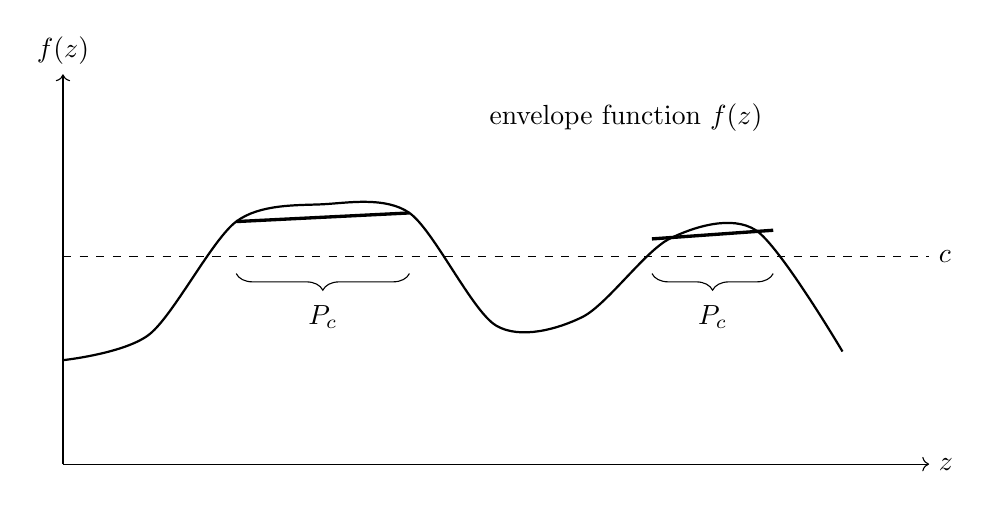
\begin{tikzpicture}[scale=1.1]

% Axes
        \draw[->] (0,0) -- (10,0) node[right] {$z$};
        \draw[->] (0,0) -- (0,4.5) node[above] {$f(z)$};

% Envelope function f(z)
        \draw[thick, smooth]
        plot coordinates {
          (0,1.2)
          (1,1.5)
          (2,2.8)
          (3,3.0)
          (4,2.9)
          (5,1.6)
          (6,1.7)
          (7,2.6)
          (8,2.7)
          (9,1.3)
        };

% Threshold
        \draw[dashed] (0,2.4) -- (10,2.4)
        node[right] {$c$};

% Highlight projected intervals
        \draw[very thick] (2.0,2.8) -- (4.0,2.9);
        \draw[very thick] (6.8,2.6) -- (8.2,2.7);

% Braces for Pc
        \draw[decorate,decoration={brace,mirror,amplitude=6pt}]
        (2.0,2.2) -- (4.0,2.2)
        node[midway,below=8pt] {$P_c$};

        \draw[decorate,decoration={brace,mirror,amplitude=6pt}]
        (6.8,2.2) -- (8.2,2.2)
        node[midway,below=8pt] {$P_c$};

% Labels
        \node at (6.5,4.0) {envelope function $f(z)$};

      \end{tikzpicture}
      \caption{Projection-induced apparent discontinuities.
      The envelope function $f(z)=\max_{x,y}\phi(x,y,z)$ is continuous, but the projected set
        $P_c=\{z\mid f(z)\ge c\}$ consists of disjoint intervals.
        The apparent fragmentation results from thresholding and does not reflect any
        discontinuity of the underlying scalar field $\phi$.}
      \label{fig:levelset_projection}
    \end{figure}

    Importantly, the apparent disjointness of $P_c$ does not imply any discontinuity of the underlying
    field $\phi$.
    Rather, it arises from the fact that only regions exceeding the chosen threshold $c$ are retained.
    The fragmentation is therefore a projection effect induced by thresholding.

  \subsubsection{Envelope Function and Threshold Visibility}

    Define the envelope function
    \begin{equation}
      f(z) = \max_{x,y} \phi(x,y,z).
    \end{equation}

    The set $P_c$ can then be written equivalently as
    \begin{equation}
      P_c = \{ z \in \mathbb{R} \mid f(z) \ge c \}.
    \end{equation}

    The function $f(z)$ is uniquely determined by $\phi$ and provides a global one-dimensional
    summary of the field's maximal amplitude along each slice of constant $z$.
    While the full three-dimensional structure of $\phi$ cannot be reconstructed from $P_c$ alone,
    the envelope function $f(z)$ encodes the emergence and disappearance of visible components as the
    threshold $c$ is varied.

    In this sense, threshold-based visualizations reveal sections of a continuous structure rather
    than discrete or independent objects.

  \subsubsection{Non-Uniqueness of Inverse Reconstruction}

    Given a projected set $P_c$ or a collection of disjoint level-set components, the inverse problem
    of reconstructing $\phi$ is not uniquely solvable.
    Multiple continuous scalar fields may share identical level sets at a given threshold.

    Additional assumptions---such as symmetry, minimal curvature, smoothness, or governing differential
    equations---are required to select a preferred reconstruction.
    The present result therefore establishes a structural constraint rather than a unique inversion.

  \subsubsection{Summary}

    Level-set visualizations of continuous scalar fields generically produce apparently disjoint
    structures when projected or thresholded.
    These structures should be understood as emergent sections of an underlying continuous field.
    The mathematical origin of this effect is independent of any specific physical interpretation,
    but it provides a natural geometric framework for understanding disjoint orbital-like patterns
    as manifestations of threshold visibility.

    While this appendix is presented independently of any physical model, the
    results apply directly to situations in which observable structures are
    defined by detection thresholds or projection procedures, as in atomic,
    optical, or imaging contexts.

    These effects are purely geometric and arise generically whenever continuous scalar
    fields are visualized through threshold-based projections (see Fig.~\ref{fig:levelset_projection}).

  \subsection{Emergent Electrodynamics from $\chi$ Dynamics}
  \label{app:emergent-electrodynamics}

  In regimes where the $\chi$ field admits a smooth geometric and weak-gradient
  description, small perturbations around a slowly varying background obey an
  effective wave equation derived from the variational formulation
  (Section~\ref{subsec:variational-formulation}):
  \begin{equation}
    \nabla \cdot
    \left(
      \frac{\nabla \chi}{\sqrt{1 - |\nabla \chi|^2 / c^2}}
    \right)
    - \frac{1}{c^2} \frac{\partial^2 \chi}{\partial t^2}
    =
    \frac{4 \pi G_{\mathrm{eff}}}{c^2} \rho_\chi .
  \end{equation}

  In the weak-field limit, $|\nabla \chi| \ll c$, this equation linearizes to
  \begin{equation}
    \nabla^2 \chi
    - \frac{1}{c^2} \frac{\partial^2 \chi}{\partial t^2}
    =
    4 \pi G_{\mathrm{eff}} \rho_\chi ,
  \end{equation}
  which admits propagating solutions interpreted as radiative disturbances of the
  $\chi$ field.

  \subsubsection*{Emergent Scalar and Vector Potentials}

    Electromagnetic-like degrees of freedom arise from the \emph{geometric structure}
    of $\chi$ perturbations rather than from independent fundamental fields.
    In regions containing charged solitonic excitations, the spatial gradients of
    $\chi$ acquire both longitudinal and transverse components.

    Accordingly, the spatial gradient of $\chi$ may be decomposed (at the effective
    level) into longitudinal and transverse parts:
    \begin{equation}
      \nabla \chi = - \nabla \phi + \mathbf{A}_{\mathrm{T}},
    \end{equation}
    where $\phi$ is an effective scalar potential and $\mathbf{A}_{\mathrm{T}}$ is a
    divergence-free vector field,
    \begin{equation}
      \nabla \cdot \mathbf{A}_{\mathrm{T}} = 0 .
    \end{equation}

    This decomposition should be understood as an effective Helmholtz projection
    induced by the topology of localized $\chi$ excitations, rather than as a
    fundamental split of degrees of freedom.
    The scalar component encodes longitudinal relaxation gradients associated with
    effective charge density, while the transverse component arises from solitonic
    configurations with non-trivial circulation.

  \subsubsection*{Topological Origin of the Vector Potential}

    The transverse component $\mathbf{A}_{\mathrm{T}}$ originates from solitonic
    configurations of $\chi$ characterized by non-vanishing loop integrals
    \begin{equation}
      \oint \nabla \chi \cdot d\mathbf{l} \neq 0 ,
    \end{equation}
    as discussed in Section~\ref{subsec:vortices}.
    Such configurations imply the existence of an effective vector potential whose
    curl is non-zero, while its divergence vanishes identically.

    The vector potential is therefore not an independent dynamical field.
    It is a derived quantity encoding the transverse sector of $\chi$ gradients,
    analogous to vorticity-induced vector fields in fluid dynamics.

  \subsubsection*{Emergent Electromagnetic Fields}

    Within this effective description, the electric and magnetic fields are defined as
    \begin{equation}
      \mathbf{E}
      =
      - \nabla \phi
      - \frac{1}{c} \frac{\partial \mathbf{A}_{\mathrm{T}}}{\partial t},
      \qquad
      \mathbf{B}
      =
      \nabla \times \mathbf{A}_{\mathrm{T}} .
    \end{equation}

    These fields satisfy the Maxwell equations:
    \begin{align}
      \nabla \cdot \mathbf{E}
      &= 4 \pi G_{\mathrm{eff}} \rho_{\mathrm{em}}, \\
      \nabla \times \mathbf{E}
      + \frac{1}{c} \frac{\partial \mathbf{B}}{\partial t}
      &= 0, \\
      \nabla \cdot \mathbf{B}
      &= 0, \\
      \nabla \times \mathbf{B}
      - \frac{1}{c} \frac{\partial \mathbf{E}}{\partial t}
      &=
      \frac{4 \pi G_{\mathrm{eff}}}{c} \mathbf{J}_{\mathrm{em}},
    \end{align}
    where $\rho_{\mathrm{em}}$ and $\mathbf{J}_{\mathrm{em}}$ denote the effective charge
    and current densities associated with solitonic $\chi$ excitations.

  \subsubsection*{Gauge Invariance}

    The decomposition of $\nabla \chi$ into scalar and transverse components is not
    unique.
    A transformation of the form
    \begin{equation}
      \phi \rightarrow \phi - \frac{1}{c} \frac{\partial \Lambda}{\partial t},
      \qquad
      \mathbf{A}_{\mathrm{T}} \rightarrow \mathbf{A}_{\mathrm{T}} + \nabla \Lambda ,
    \end{equation}
    leaves the observable fields $\mathbf{E}$ and $\mathbf{B}$ invariant.

    This emergent $U(1)$ gauge symmetry reflects the relational nature of $\chi$:
    only differences of gradients have operational meaning, while the absolute
    potential is unobservable
    (Section~\ref{subsec:relational-foundation-pointer}).

  \subsubsection*{Interpretational Status}

    The Maxwell-like structure derived here is not fundamental.
    It arises as a universal effective description of transverse $\chi$ perturbations
    in regimes where solitonic topology and weak gradients coexist.
    Electromagnetism therefore appears as a geometric manifestation of the relational
    and topological structure of the $\chi$ field, rather than as an independent
    interaction mediated by elementary gauge fields.


    \section{Appendix B: Conceptual Extensions of Cosmochrony — Particles, Quantum Phenomena, and Classical Limits}
  \label{sec:appendix-conceptual}
  This appendix explores the conceptual and phenomenological extensions of the Cosmochrony framework, including:
  \begin{itemize}
    \item The nature of the $\chi$ field and its interpretation as a geometric substrate (Section~\ref{subsec:nature-chi}).
    \item Topological solitons as particle solutions, with explicit constructions for fermions and bosons (Sections~\ref{subsec:topological_solitons}--\ref{subsec:4pi_soliton}).
    \item The emergence of classical limits and the status of the formulation (Sections~\ref{subsec:classical-limits}--\ref{subsec:status-formulation}).
    \item Perspectives on deriving the mass spectrum from $\chi$-field dynamics (Section~\ref{subsec:perspectives_mass_spectrum}).
  \end{itemize}
  These extensions bridge the gap between the mathematical foundations (Appendix~\ref{sec:appendix-math}) and cosmological observations (Appendix~\ref{sec:appendix-cosmo}).

  \subsection{Interpretative Status of the $\chi$ Field}
  \label{subsec:nature-chi}

  This subsection does not introduce new postulates regarding the $\chi$ field.
  Its purpose is purely interpretative: to clarify how $\chi$ should be understood
  \emph{once the framework has been established}, and to prevent several common
  misreadings suggested by conventional field-theoretic language.

  In the main text, $\chi$ is often written in the form $\chi(x^\mu)$ and manipulated
  using continuous differential operators.
  This notation should not be taken to imply that $\chi$ is a physical field
  propagating \emph{within} a pre-existing spacetime manifold.
  Rather, spacetime coordinates serve only as convenient labels for organizing
  relational information in regimes where a stable geometric description has emerged.

  Fundamentally, $\chi$ encodes a relational scale of relaxation from which notions
  such as duration, distance, and causal ordering are reconstructed.
  The apparent embedding of $\chi$ in spacetime is therefore representational,
  not ontological.
  The manifold description is a secondary construct, introduced only after the
  relaxation dynamics of $\chi$ has reached sufficient regularity to admit a
  geometric interpretation.

  This distinction mirrors the use of continuum variables in hydrodynamics or
  elasticity theory.
  Just as a velocity field does not exist independently of the underlying molecular
  interactions, $\chi(x^\mu)$ does not represent a fundamental spacetime field.
  It summarizes collective relational properties of the substrate once coarse
  graining becomes meaningful.

  In this sense, $\chi$ should not be interpreted as:
  \begin{itemize}
    \item a matter field living on spacetime,
    \item a dynamical scalar coupled to a pre-existing metric,
    \item or a hidden-variable replacement for the quantum wavefunction.
  \end{itemize}

  Instead, $\chi$ constitutes the pre-geometric quantity from which spacetime
  structure, effective fields, and physical observables emerge through projection
  and coarse graining.
  The use of continuous fields, Lagrangians, and differential equations throughout
  this work reflects practical representational choices rather than fundamental
  commitments.

  This interpretative clarification is particularly important for understanding the
  role of localized excitations, solitonic structures, and effective fields discussed
  in the remainder of this appendix.
  These constructions should be read as regime-dependent invariants of the underlying
  $\chi$ dynamics, not as evidence that $\chi$ itself decomposes into independently
  propagating physical entities.

  In summary, the $\chi$ field is not a field \emph{in} spacetime.
  Spacetime is an emergent bookkeeping structure \emph{for} $\chi$ once its relational
  dynamics becomes sufficiently regular.
  This asymmetry is essential to the ontological parsimony of the Cosmochrony
  framework and underlies its reinterpretation of geometry, matter, and quantum
  phenomena.

  \subsection{Topological Configurations of the \(\chi\) Field: Solitons as Particles}
  \label{app:topological_solitons}

  \paragraph{Status of this construction.}
    The solitonic configurations described in this section are not introduced as
    fundamental degrees of freedom of Cosmochrony.
    They constitute \emph{effective geometric models} intended to illustrate how
    particle-like properties may emerge from stable configurations of the $\chi$
    field once a continuum and orientable geometric description becomes applicable.

    At the fundamental level, Cosmochrony does not assume a pre-existing spatial
    manifold, metric, or differential structure.
    A fully relational formulation, free of geometric presuppositions, is presented
    separately in Appendix~\ref{app:relational_formulation}.
    The present constructions should therefore be understood as phenomenological
    representations valid in the emergent geometric regime.

  In Cosmochrony, particles are interpreted as \textbf{topologically stable solitons} of the \(\chi\) field, where their
  properties---such as \textbf{spin, charge, and mass}---emerge from the \textbf{local deformation of \(\chi\)} and its
  topological structure.
  Below, we classify these configurations and explicitly link them to particle properties, emphasizing how
  \textbf{charge arises from the modulation of \(\chi\)'s relaxation}.

  \subsubsection{Charge as Local Deformation of \(\chi\)}
    The \textbf{sign of a particle's charge} (positive or negative) is determined by how it deforms the \(\chi\)
    field:
    \begin{itemize}
      \item A \textbf{positive charge} corresponds to a \textbf{local extension of \(\chi\)} (a "peak"), which resists relaxation and repels other positive charges (as two peaks cannot merge).
      \item A \textbf{negative charge} corresponds to a \textbf{local contraction of \(\chi\)} (a "trough"), which attracts positive charges (as a peak and trough can annihilate or merge).
    \end{itemize}
    This geometric interpretation explains \textbf{Coulomb-like interactions}
    without invoking a fundamental electromagnetic field, but as a consequence of \(\chi\) dynamics.

    \begin{figure}[h]
      \centering
      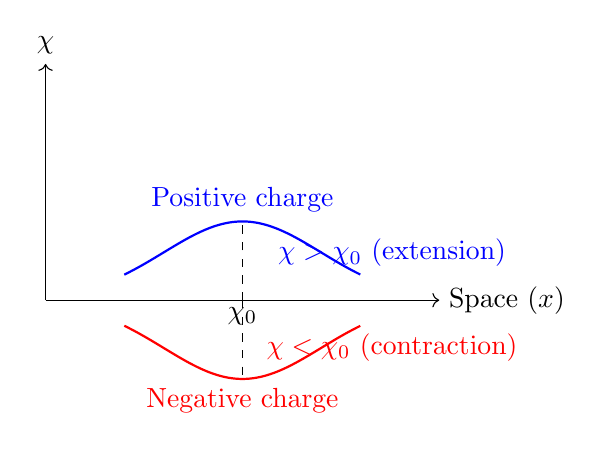
\begin{tikzpicture}[x=2cm, y=2cm]
        % Axes
        \draw[->] (0,0) -- (2.5,0) node[right] {Space (\(x\))};
        \draw[->] (0,0) -- (0,1.5) node[above] {$\chi$};
        % Positive charge: Peak in chi
        \draw[thick, blue, domain=0.5:2, samples=100] plot (\x, {0.5*exp(-2*(\x-1.25)^2)});
        \node[blue, above] at (1.25, 0.5) {Positive charge};
        \draw[dashed] (1.25,0) -- (1.25,0.5);
        \node at (1.25,-0.1) {$\chi_0$};
        % Negative charge: Trough in chi
        \draw[thick, red, domain=0.5:2, samples=100] plot (\x, {-0.5*exp(-2*(\x-1.25)^2)});
        \node[red, below] at (1.25, -0.5) {Negative charge};
        \draw[dashed] (1.25,0) -- (1.25,-0.5);
        % Labels
        \node[blue] at (2.2, 0.3) {$\chi > \chi_0$ (extension)};
        \node[red] at (2.2, -0.3) {$\chi < \chi_0$ (contraction)};
      \end{tikzpicture}
      \caption{
        Local deformations of the $\chi$ field representing positive (peak) and negative (trough) charges.
        The extension or contraction of $\chi$ relative to its background value $\chi_0$ determines the sign of the
        charge and the nature of its interactions (This figure and following ones are schematic representations intended
        to illustrate the geometric and topological structure of $chi$-field excitations, not numerical solutions of the
        dynamical equations.).
      }
      \label{fig:chi_charges}
    \end{figure}


  \subsubsection{Vortices (Charged Particles with Spin)}
    Vortices in the \(\chi\) field are characterized by a quantized winding number \(n\):
    \[
      n = \frac{1}{2\pi} \oint \nabla \arg(\chi) \cdot d\mathbf{l}.
    \]
    The \textbf{charge of the vortex} is determined by the \textbf{sign of its deformation}:
    \begin{itemize}
      \item For \(n > 0\), the vortex creates a \textbf{local extension of \(\chi\)} (positive charge).
      \item For \(n < 0\), the vortex creates a \textbf{local contraction of \(\chi\)} (negative charge).
    \end{itemize}
    The energy of the vortex scales with \(n^2\), reflecting the \textbf{mass of the particle}
    , while its winding determines the \textbf{spin} (e.g., \(n=1\) for spin-1 bosons).

    \begin{figure}[h]
      \centering
      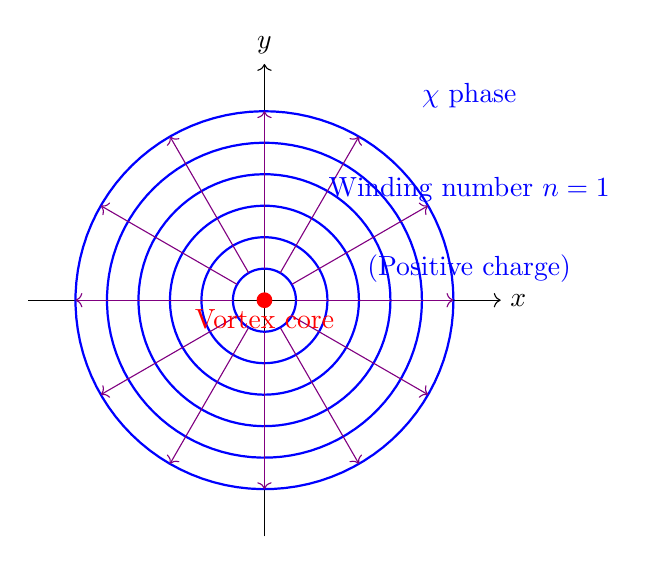
\begin{tikzpicture}[x=2cm, y=2cm]
        % Axes
        \draw[->] (-1.5,0) -- (1.5,0) node[right] {$x$};
        \draw[->] (0,-1.5) -- (0,1.5) node[above] {$y$};
        % Vortex field lines (streamlines of chi)
        \foreach \r in {0.2, 0.4, ..., 1.2} {
          \draw[blue, thick, domain=0:6.28, samples=100, variable=\t]
          plot ({\r*cos(\t r)}, {\r*sin(\t r)});
        }
        % Chi field phase (color gradient)
        \foreach \t in {0, 30, ..., 330} {
          \draw[red!50!blue, ->, domain=0.2:1.2, samples=20, variable=\r]
          plot ({\r*cos(\t)}, {\r*sin(\t)});
        }
        % Core of the vortex
        \fill[red] (0,0) circle (0.05);
        \node[red, below] at (0,0) {Vortex core};
        % Labels
        \node[blue] at (1.3, 1.3) {$\chi$ phase};
        \node[blue] at (1.3, 0.7) {Winding number $n=1$};
        \node[blue] at (1.3, 0.2) {(Positive charge)};
      \end{tikzpicture}
      \caption{
        Vortex configuration in the $\chi$ field, characterized by a winding number $n=1$.
        The circular phase gradient (arrows) represents the spin of the particle, while the core (red dot) corresponds to a localized deformation of $\chi$ (positive charge).
        Such configurations model charged bosons with quantized angular momentum.
      }
      \label{fig:chi_vortex}
    \end{figure}

  \subsubsection{Skyrmions (Fermions with Charge and Spin-1/2)}
    Skyrmions are 3D solitons with a topological charge \(Q\):
    \[
      Q = \frac{1}{4\pi} \int \mathbf{n} \cdot (\partial_x \mathbf{n} \times \partial_y \mathbf{n}) \, dx \, dy,
    \]
    where \(\mathbf{n} = \chi / |\chi|\).
    The \textbf{charge of the skyrmion} is linked to the
    \textbf{polarity of its \(\chi\) deformation}:
    \begin{itemize}
      \item A skyrmion with \(Q = +1\) and a \textbf{peak in \(\chi\)} represents a
      \textbf{positively charged fermion} (e.g., proton).
      \item A skyrmion with \(Q = -1\) and a \textbf{trough in \(\chi\)} represents a
      \textbf{negatively charged fermion} (e.g., electron).
    \end{itemize}
    The \(4\pi\)-periodicity of skyrmions under rotations explains their \textbf{spin-1/2}
    nature, while the deformation of \(\chi\) accounts for their charge.

    \begin{figure}[h]
      \centering
      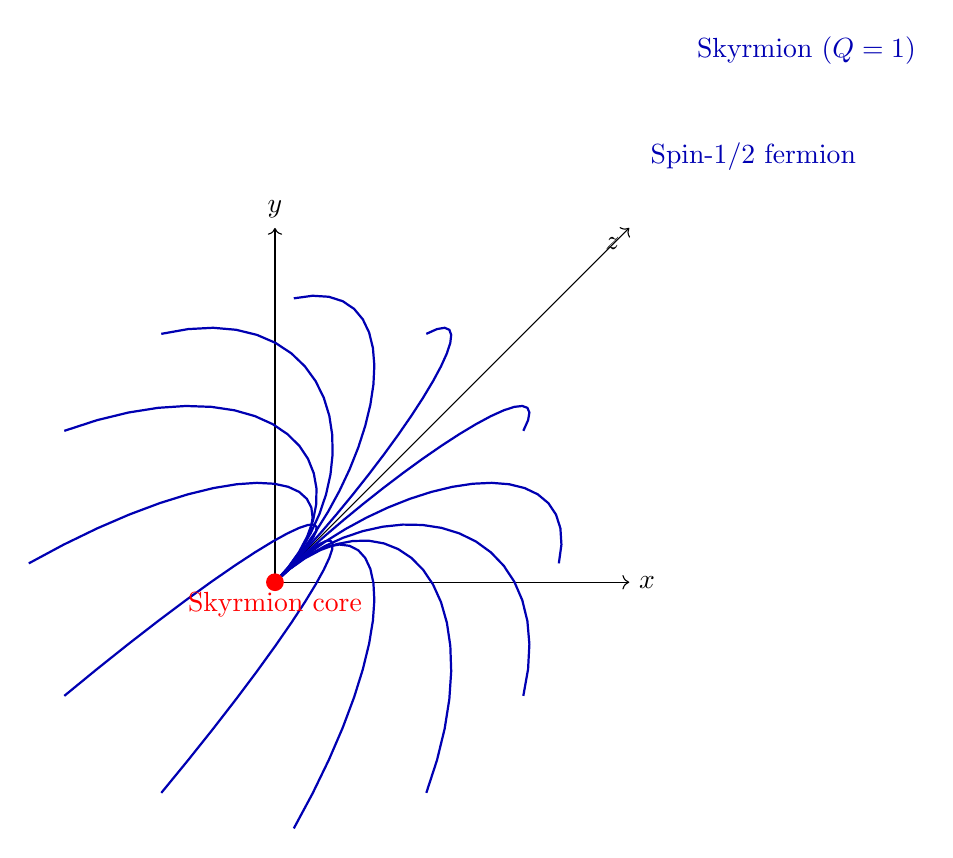
\begin{tikzpicture}[x=1.5cm, y=1.5cm, z=1.5cm, scale=1.5]
        % Axes
        \draw[->] (0,0,0) -- (2,0,0) node[right] {$x$};
        \draw[->] (0,0,0) -- (0,2,0) node[above] {$y$};
        \draw[->] (0,0,0) -- (0,0,2) node[below left] {$z$};
        % Skyrmion field (simplified representation)
        \foreach \phi in {0, 30, ..., 330} {
          \draw[blue!70!black, thick, domain=0:1.5, samples=20, variable=\r]
          plot ({\r*sin(deg(\r))*cos(\phi)}, {\r*sin(deg(\r))*sin(\phi)}, {\r*cos(deg(\r))});
        }
        % Core and labels
        \fill[red] (0,0,0) circle (0.05);
        \node[red, below] at (0,0,0) {Skyrmion core};
        \node[blue!70!black] at (1.5, 1.5, 1.5) {Skyrmion ($Q=1$)};
        \node[blue!70!black] at (1.5, 1.2, 1.2) {Spin-1/2 fermion};
      \end{tikzpicture}
      \caption{
        Skyrmion configuration in the $\chi$ field, with topological charge $Q=1$.
        The 3D structure reflects the fermionic nature of the particle (spin-1/2), where the core (red dot) represents a localized excitation of $\chi$.
        Skyrmions provide a geometric model for fermions, with their charge determined by the polarity of the $\chi$ deformation.
      }
      \label{fig:chi_skyrmion}
    \end{figure}

  \subsubsection{Summary: Topology and Charge}
    The relationship between topology and charge in Cosmochrony is summarized in ~\ref{tab:solitons_charge}

    \begin{table}[htbp]
      \centering
      \caption{Topological Solitons, Charge, and \(\chi\) Deformation}
      \label{tab:solitons_charge}
      \begin{tabular}{|c|c|c|c|}
        \hline
        \textbf{Soliton Type} & \textbf{Topological Invariant} & \textbf{\(\chi\) Deformation} &
        \textbf{Particle Property} \\
        \hline
        Vortex & Winding number \(n\) & Peak (\(n>0\)) or trough (\(n<0\)) & Charge
        \(\propto n\), spin \(\propto |n|\) \\
        Skyrmion & Charge \(Q\) & Peak (\(Q>0\)) or trough (\(Q<0\)) & Charge
        \(\propto Q\), spin-1/2 \\
        \hline
      \end{tabular}
    \end{table}

  \subsection{Soliton Energy and Structural Mass Scaling}
  \label{subsec:soliton_energy_mass}

  \paragraph{Status and scope of this analysis.}
    This subsection presents a \emph{quantitative but non-numerical} analysis of the
    effective mass associated with localized solitonic configurations arising in the
    \emph{projectable regime} of Cosmochrony.
    The objective is not to reproduce the observed particle mass spectrum, but to
    identify robust scaling relations, hierarchy constraints, and structural dependencies
    that emerge independently of microscopic details.

    No claim is made that the expressions introduced below define a fundamental
    Hamiltonian or Lagrangian for the \(\chi\) field.
    A fully predictive derivation of particle masses would require a complete effective
    theory incorporating projection dynamics, interaction channels, and renormalization
    effects, which lies beyond the scope of the present work.

    All energetic and spectral quantities discussed in this section refer exclusively
    to the effective projected field \(\chi_{\mathrm{eff}}\).
    The fundamental \(\chi\) field itself does not admit an energy functional or mass
    interpretation.

  \paragraph{Mass as integrated resistance to relaxation.}
    Within Cosmochrony, the mass of a localized excitation is interpreted as a measure of
    the total \emph{resistance to relaxation} imposed by the configuration on the
    surrounding \(\chi_{\mathrm{eff}}\) field.

    Once an effective geometric description applies, this resistance can be summarized
    by an effective diagnostic functional
    \begin{equation}
      M_{\mathrm{eff}} \;\propto\;
      \int_{\mathcal{V}}
      \left[
        \mathcal{T}\!\left(\nabla \chi_{\mathrm{eff}}\right)
        + \mathcal{U}\!\left(\chi_{\mathrm{eff}}\right)
      \right]
      \, d^3x ,
    \end{equation}
    where:
    \begin{itemize}
      \item \(\mathcal{T}\) encodes gradient-induced resistance associated with spatial
      inhomogeneities of \(\chi_{\mathrm{eff}}\),
      \item \(\mathcal{U}\) represents effective nonlinear stabilization terms arising
      from collective relaxation constraints.
    \end{itemize}

    This expression should be understood as a \emph{coarse-grained measure} of structural
    complexity rather than as a fundamental energy density.
    It quantifies how strongly a localized configuration delays or distorts the global
    relaxation of the projected field.

  \paragraph{Scaling with soliton size and internal structure.}
    Consider a localized solitonic configuration characterized by:
    \begin{itemize}
      \item a typical spatial extent \(\ell\),
      \item a characteristic deformation amplitude \(\Delta \chi_{\mathrm{eff}}\).
    \end{itemize}

    Dimensional analysis then yields the generic scaling
    \begin{equation}
      M_{\mathrm{eff}} \;\sim\;
      \ell^3
      \left[
        \frac{(\Delta \chi_{\mathrm{eff}})^2}{\ell^2}
        + V_{\mathrm{eff}}(\Delta \chi_{\mathrm{eff}})
      \right],
    \end{equation}
    where \(V_{\mathrm{eff}}\) denotes an effective nonlinear stabilization potential
    generated by projection and relaxation constraints.

    For simple kink-like configurations, the balance between gradient resistance and
    nonlinear stabilization dynamically fixes the soliton width \(\xi\).
    In this regime, the effective mass scale may be written schematically as
    \begin{equation}
      M_{\mathrm{eff}} \;\sim\;
      \sqrt{\lambda_{\mathrm{eff}}}\,\xi\,\chi_c^2 ,
    \end{equation}
    where:
    \begin{itemize}
      \item \(\chi_c\) denotes the characteristic local relaxation scale,
      \item \(\lambda_{\mathrm{eff}}\) is an emergent, configuration-dependent stiffness
      parameter.
    \end{itemize}

    Neither \(\chi_c\) nor \(\lambda_{\mathrm{eff}}\) should be interpreted as
    fundamental constants.
    They summarize collective properties of the projected relaxation regime.

  \paragraph{Structural stabilization and finite mass.}
    When stabilization arises from a balance between gradient-induced resistance and
    nonlinear relaxation constraints, the soliton size \(\ell\) is dynamically fixed.
    This mechanism ensures that localized excitations possess a finite and stable
    effective mass without the need for fine-tuning.

    Different classes of solitonic configurations (kinks, vortices, knotted or linked
    structures) involve distinct internal organizations of \(\chi_{\mathrm{eff}}\).
    As a result, their effective masses exhibit different scaling behaviors with respect
    to \(\ell\) and \(\Delta \chi_{\mathrm{eff}}\).

    This implies that mass hierarchies arise \emph{structurally} rather than through
    arbitrary parameter choices.

  \paragraph{Topological classes and mass hierarchy.}
    The effective mass depends not only on the spatial extent of a soliton but also on
    its topological class.
    Configurations characterized by higher winding, linking, or covering indices
    necessarily involve increased internal gradients and more complex relaxation
    constraints.

    Consequently, masses associated with different topological families obey ordering
    relations of the form
    \begin{equation}
      M_{n+1} \;>\; M_n ,
    \end{equation}
    where \(n\) labels an effective topological invariant.
    This establishes a natural mechanism for discrete mass hierarchies without introducing
    ad hoc mass parameters.

  \paragraph{Spectral interpretation.}
    From a spectral perspective, localized excitations correspond to bound modes of the
    linearized relaxation operator around a solitonic background configuration of
    \(\chi_{\mathrm{eff}}\).

    The effective mass is then controlled by the lowest nontrivial eigenvalue of this
    operator,
    \begin{equation}
      M_{\mathrm{eff}} \;\sim\; \lambda_{\min}^{-1},
    \end{equation}
    where \(\lambda_{\min}\) denotes the smallest positive eigenvalue governing the
    stability of the configuration.

    This formulation emphasizes that mass is fundamentally a \emph{spectral property}
    of the relaxation dynamics rather than an intrinsic attribute of a particle-like
    object.

  \paragraph{Robustness and universality.}
    The scaling relations derived above depend only on generic features of the projected
    \(\chi\) dynamics—locality, monotonic relaxation, and nonlinear stabilization—and
    are therefore expected to be robust against modifications of microscopic details.

    While specific numerical values of particle masses cannot be fixed at this level,
    the existence of discrete, ordered, and stable mass scales emerges as a structural
    prediction of the framework.

  \paragraph{Order-of-magnitude consistency.}
    Although the present analysis does not aim to reproduce the observed particle mass
    spectrum, it is instructive to examine whether the structural parameters entering the
    solitonic energy scale admit values compatible with known masses.

    For a simple kink-like configuration with characteristic width
    \(\lambda_{\mathrm{eff}}^{-1}\) and amplitude set by the local relaxation scale
    \(\chi_c\), the effective rest energy scales as
    \begin{equation}
      E_{\mathrm{sol}} \;\sim\; \chi_c^2 \lambda_{\mathrm{eff}},
    \end{equation}
    up to dimensionless shape-dependent factors of order unity.

    Identifying this energy with the electron rest mass,
    \(E_{\mathrm{sol}} \sim m_e c^2 \approx 0.511\,\mathrm{MeV}\),
    and expressing all quantities in natural units (\(\hbar = c = 1\)),
    one finds that reproducing the electron mass requires
    \begin{equation}
      \lambda_{\mathrm{eff}} \;\sim\; 10^{-44},
    \end{equation}
    for \(\chi_c\) normalized near the Planck scale.

    Such an extremely small value should not be interpreted as a fundamental coupling.
    Rather, it strongly suggests that \(\lambda_{\mathrm{eff}}\) is dynamically generated
    through collective relaxation, projection effects, and topological constraints of
    the \(\chi\) field.

  \paragraph{Summary.}
    Localized solitonic configurations of the projected field \(\chi_{\mathrm{eff}}\)
    naturally possess finite effective masses determined by their size, internal
    organization, and topological class.
    Rather than predicting specific numerical values, Cosmochrony constrains the
    \emph{scaling, ordering, and stability} of masses through geometric and spectral
    principles.

    This structural quantitativity provides a coherent foundation for future extensions
    toward a fully predictive effective theory, without compromising the pre-geometric
    nature of the fundamental \(\chi\) field.

  \subsection{Example: \(4\pi\)-Periodic Soliton and Spin-1/2}
  \label{subsec:4pi_soliton}

  To illustrate how a \(4\pi\)
  -periodic soliton can represent a spin-1/2 particle, consider a 1D soliton solution for the \(\chi\)
  field with a phase twist. Let \(\chi(x)\) be a complex field defined as:

  \[
    \chi(x) = \eta \tanh(\kappa x) e^{i \theta(x)},
  \]

  where \(\eta\) is the amplitude, \(\kappa\) determines the soliton's width, and \(\theta(x)\)
  is the phase. For a spin-1/2 particle, the phase \(\theta(x)\) must satisfy:

  \[
    \theta(x + 2\pi) = \theta(x) + \pi, \quad \theta(x + 4\pi) = \theta(x) + 2\pi.
  \]

  This \(4\pi\)-periodicity reflects the double-valuedness of spinors under rotations.

  \subsubsection{Explicit Construction of a \(4\pi\)-Periodic Soliton}

    Define the phase \(\theta(x)\) as:

    \[
      \theta(x) = \frac{x}{2},
    \]

    so that a full rotation \(x \to x + 4\pi\) returns the phase to its original value:

    \[
      \theta(x + 4\pi) = \frac{x + 4\pi}{2} = \theta(x) + 2\pi.
    \]

    The soliton solution is then:

    \[
      \chi(x) = \eta \tanh(\kappa x) e^{i x/2}.
    \]

    This soliton has the following properties:
    \begin{itemize}
      \item It is localized around \(x = 0\), with \(\chi(x) \to 0\) as \(|x| \to \infty\).
      \item The phase winds by \(\pi\) as \(x\) goes from \(-\infty\) to \(+\infty\), but a full \(2\pi\)
      rotation of the soliton requires \(x \to x + 4\pi\), reflecting the spin-1/2 nature.
    \end{itemize}

  \subsubsection{Topological Interpretation}

    The \(4\pi\)-periodicity of the soliton is a manifestation of its \textbf{topological winding number}
    . For a closed loop in space, the phase change \(\Delta \theta\) is given by:

    \[
      \Delta \theta = \oint \nabla \theta \cdot d\mathbf{l} = 2\pi n,
    \]

    where \(n\) is the winding number. For a spin-1/2 particle, the effective winding is \(n = 1/2\)
    , but since the phase must be single-valued in space, the soliton must traverse the loop twice to return to
    its original state, hence the \(4\pi\)-periodicity.

  \subsubsection{Connection to Quantum Statistics}

    The \(4\pi\)-periodicity of the soliton directly implies that it obeys \textbf{fermionic statistics}:
    \begin{itemize}
      \item Under a \(2\pi\) rotation, the wavefunction of the soliton acquires a phase of \(e^{i\pi} = -1\)
      , which is the hallmark of a fermion.
      \item This explains the \textbf{Pauli exclusion principle}
      : two identical solitons cannot occupy the same state because their wavefunctions would interfere
      destructively due to the \(-1\) phase factor.
    \end{itemize}

    \begin{figure}[h]
      \centering
      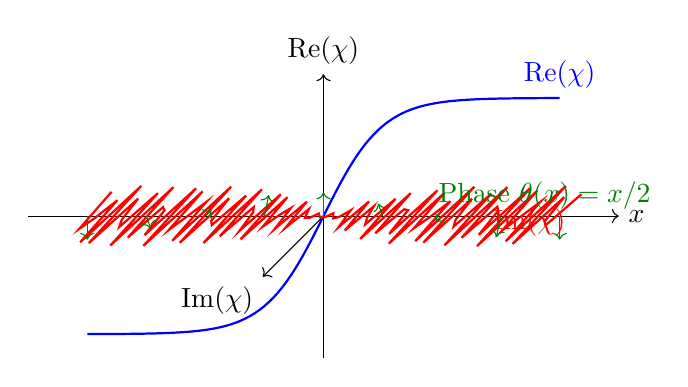
\begin{tikzpicture}[x=1.5cm, y=1.5cm]
        % Axes
        \draw[->] (-2.5,0) -- (2.5,0) node[right] {$x$};
        \draw[->] (0,-1.2) -- (0,1.2) node[above] {$\Re(\chi)$};
        \draw[->] (0,0) -- (0,0,2) node[below left] {$\Im(\chi)$};

        % Real part of chi
        \draw[thick, blue, domain=-2:2, samples=100] plot (\x, {tanh(2*\x)}, 0);
        \node[blue, above] at (2, 1, 0) {$\Re(\chi)$};

        % Imaginary part of chi
        \draw[thick, red, domain=-2:2, samples=100] plot (\x, 0, {tanh(2*\x)*sin(deg(90*\x))});
        \node[red, above] at (2, 0, 1) {$\Im(\chi)$};

        % Phase arrows
        \foreach \x in {-2, -1.5, ..., 2} {
          \pgfmathsetmacro{\phase}{90*\x}
          \draw[green!50!black, ->] (\x, 0, 0) -- (\x, {0.2*cos(\phase)}, {0.2*sin(\phase)});
        }
        \node[green!50!black] at (2, 0.3, 0.5) {Phase $\theta(x) = x/2$};
      \end{tikzpicture}
      \caption{
        Visualization of a \(4\pi\)-periodic soliton representing a spin-1/2 particle.
        The real part \(\Re(\chi)\) (blue) and imaginary part \(\Im(\chi)\) (red) of the \(\chi\) field are shown,
        along with the local phase (green arrows).
        The phase winds by \(\pi\) over the spatial extent of the soliton, but a full \(2\pi\)
        rotation of the soliton requires a \(4\pi\) change in phase, reflecting its fermionic nature.
      }
      \label{fig:4pi_soliton}
    \end{figure}

  \subsection{Relation to Classical Limits}
  \label{subsec:classical-limits}

  In Cosmochrony, the emergence of classical behavior does not correspond to the
  introduction of an independent theoretical layer.
  Instead, classical physics arises as a \emph{dynamical regime} of the same underlying
  scalar structure, characterized by smoothness, dilution of localized excitations,
  and the suppression of topological and relational effects.

  \paragraph{Weakly structured regime and effective linearization.}
    In regimes where the fundamental field \(\chi\) admits a stable projective
    representation and where its effective projection \(\chi_{\mathrm{eff}}\) varies
    slowly over large scales, localized excitations become dilute and weakly interacting.
    Under these conditions, the dynamics of \(\chi_{\mathrm{eff}}\) can be linearized
    around a quasi-homogeneous background configuration.

    In this regime, small perturbations propagate as weak disturbances on an effectively
    flat geometric background.
    Superposition, approximate locality, and linear wave propagation emerge as effective
    properties of the coarse-grained relaxation dynamics.
    This reproduces the operational content of classical field theories and of quantum
    field theories formulated on Minkowski spacetime.

    This correspondence should be understood as an \emph{effective recovery} rather than
    as an ontological reduction.
    Cosmochrony does not reduce to standard quantum field theory; rather, standard field
    theories appear as limiting descriptions valid when relational structure becomes
    dynamically inert.

  \paragraph{Suppression of relational and topological effects.}
    In the weakly structured regime, topological constraints associated with solitonic
    configurations are either absent or dynamically irrelevant.
    The configuration space effectively factorizes, and collective relaxation dominates
    over localized structural organization.
    As a result, particle-like excitations behave as approximately independent degrees
    of freedom, and classical intuition becomes applicable.

    The classical limit therefore corresponds to a regime in which the relational content
    of \(\chi\) is present but operationally inaccessible, masked by coarse-graining and
    scale separation.

  \paragraph{Nonlinear regime and effective curvature.}
    Conversely, in regimes of strong spatial variation of \(\chi_{\mathrm{eff}}\) or high
    density of localized excitations, nonlinear effects dominate the dynamics.
    Large gradients locally constrain relaxation, inducing effective curvature, time
    dilation, and horizon-like behavior in the emergent geometric description.

    These regimes reproduce the phenomenology associated with curved spacetime,
    gravitational collapse, and strong-field effects, while remaining governed by the same
    underlying scalar dynamics.
    No additional gravitational degrees of freedom are introduced; curvature emerges as
    a collective response of the relaxation structure of \(\chi_{\mathrm{eff}}\).

  \paragraph{Meaning of the classical limit in Cosmochrony.}
    The classical limit in Cosmochrony is therefore not defined by \(\hbar \to 0\), nor by
    the suppression of quantum postulates.
    It corresponds to a regime in which:
    \begin{itemize}
      \item the effective projection \(\chi_{\mathrm{eff}}\) is smooth and slowly varying,
      \item localized excitations are dilute and weakly correlated,
      \item topological and relational constraints are dynamically suppressed,
      \item coarse-graining yields stable geometric descriptions.
    \end{itemize}

    In this regime, classical spacetime and standard field dynamics emerge as reliable,
    approximate descriptions.
    Their validity reflects not fundamental structure, but the stability of a particular
    relaxation regime of the underlying \(\chi\) field.

  \subsection{Status of the Formulation}
  \label{subsec:status-formulation}

  The formulation presented in this work should be understood as a
  \emph{minimal yet structurally complete} theoretical framework.
  Its ontological commitments, dynamical principles, and interpretative structure
  are fully specified at the conceptual level, even though several technical
  developments remain open.

  In particular, a fully covariant action principle formulated solely in terms of
  the fundamental \(\chi\) dynamics, as well as a systematic quantization procedure,
  have not yet been derived in their final and definitive form.
  These missing elements should not be interpreted as conceptual deficiencies.
  Rather, they correspond to technical extensions required to interface a
  fundamentally relational and pre-geometric framework with conventional
  variational and quantum formalisms that presuppose spacetime structure.

  Crucially, the absence of a finalized action or quantization scheme does not
  obstruct the recovery of known physical phenomenology.
  Throughout this work, general relativity and quantum field theory emerge as
  \emph{effective, coarse-grained descriptions} valid within specific dynamical
  regimes of the projected field \(\chi_{\mathrm{eff}}\).
  They are not introduced as independent axioms, but arise as stable limits of the
  underlying relaxation dynamics.

  The present formulation therefore occupies a well-defined intermediate status.
  It is not intended as a closed or final theory, nor as a phenomenological model
  tuned to reproduce specific experimental data.
  Instead, it provides a coherent ontological and dynamical foundation from which
  both geometric and quantum structures can emerge, while remaining open to future
  refinements that may enhance its mathematical completeness, formal elegance, and
  predictive scope.

  In this sense, Cosmochrony should be viewed as a foundational framework rather
  than as a fully developed effective field theory: its primary contribution lies
  in clarifying \emph{what is fundamental} and \emph{how known physical structures
can arise}, rather than in prescribing their final mathematical implementation.

  \subsection{Soliton and Particle Solutions}
  \label{subsec:soliton-and-particle-solutions}

  Within the Cosmochrony framework, elementary particles are interpreted as stable
  or metastable localized configurations arising in the \emph{projectable regime}
  of the scalar field \(\chi\).
  These configurations, hereafter referred to as \(\chi\)-solitons, emerge from
  nonlinear self-organization of the relaxation dynamics and persist as localized
  resistances to global relaxation.

  This interpretation does not rely on the postulation of additional fundamental
  degrees of freedom.
  The only fundamental entity is the scalar field \(\chi\), which is not defined on
  spacetime.
  Spatial localization, energy, and particle-like persistence arise only once an
  effective geometric projection \(\chi_{\mathrm{eff}}\) becomes applicable.

  While the fundamental field is scalar, certain solitonic configurations of
  \(\chi_{\mathrm{eff}}\) possess a nontrivial internal organization that cannot be
  faithfully encoded by a single real scalar variable.
  In particular, configurations characterized by internal cyclic structure,
  nontrivial winding, and \(4\pi\)-periodicity exhibit transformation properties
  that require a double-valued representation under effective rotations.

  In such cases, an effective spinorial description becomes unavoidable.
  This does not imply the existence of fundamental spinor fields.
  Rather, spinorial variables arise as \emph{collective descriptors} encoding the
  internal topology and spectral structure of fermionic \(\chi\)-solitons.

  At the phenomenological level, these excitations admit a representation in terms
  of Dirac spinors.
  This representation should be understood as an emergent and coarse-grained
  description of the internal degrees of freedom of \(\chi\)-solitons, not as an
  ontological extension of the theory.
  Within this regime, the Dirac equation appears as the minimal effective dynamical
  structure compatible with:
  \begin{itemize}
    \item approximate locality in the projected geometric description,
    \item effective relativistic covariance,
    \item and the topological constraints associated with \(4\pi\)-periodic
    configurations.
  \end{itemize}

  From this perspective, the Dirac structure does not introduce new fundamental
  entities.
  It provides a compact and universal encoding of the internal topology, spectral
  stability, and transformation behavior of fermionic solitons.
  Spin, fermionic statistics, and exclusion behavior arise as effective consequences
  of the nontrivial configuration space of these scalar-field excitations, rather
  than as independent postulates.

  The existence and stability of \(\chi\)-solitons impose structural constraints on
  the effective self-interaction functional governing the projected dynamics.
  Although the explicit form of this functional remains undetermined, it must satisfy
  the following minimal requirements:
  \begin{enumerate}
    \item the support of localized configurations with finite effective mass,
    \item dynamical stability under small perturbations,
    \item and the existence of topologically inequivalent sectors corresponding to
    distinct classes of particle-like excitations.
  \end{enumerate}

  The detailed derivation of effective Dirac dynamics from fluctuations around
  \(\chi\)-soliton backgrounds, as well as the emergence of a realistic mass
  spectrum, remains an open mathematical problem.
  These issues are addressed at a programmatic and illustrative level in
  Sections~\ref{app:topological_solitons}--\ref{subsec:4pi_soliton} and further
  discussed in Appendix~\ref{subsec:perspectives_mass_spectrum}.

  \subsection{Perspectives: Towards a Derivation of the Proton-to-Electron Mass Ratio}
  \label{subsec:perspectives_mass_spectrum}

  The proton-to-electron mass ratio is one of the most precisely measured dimensionless quantities in physics.
  Within the Cosmochrony framework, the purpose of this section is not to derive this
  value from first principles, but to clarify how such a ratio could emerge
  \emph{structurally} from the spectral and topological organization of localized
  solitonic excitations of the projected field \(\chi_{\mathrm{eff}}\).

  The discussion should therefore be understood as a minimal and exploratory spectral ansatz.
  Its aim is to identify the relevant mechanisms, constraints, and scaling relations
  that any successful derivation would have to satisfy, rather than to provide a complete microscopic calculation.

  \subsubsection*{Spectral Stability Hypothesis}

    Let \(\chi_{\mathrm{sol}}\) denote a stationary localized configuration arising in
    the projectable regime of the \(\chi\) dynamics.
    Small perturbations \(\delta\chi_{\mathrm{eff}}\) around this background are
    governed, at the coarse-grained level, by a linear stability operator
    \(\mathcal{L}_{\mathrm{sol}}\), defined as the second variation of an effective localization functional.

    Normal modes satisfy the eigenvalue problem
    \begin{equation}
      \mathcal{L}_{\mathrm{sol}} \psi_n = \lambda_n \psi_n .
    \end{equation}

    The eigenvalues \(\lambda_n\) characterize the resistance of the soliton to
    localized deformations.
    They encode intrinsic stiffness scales associated with the internal organization
    of the solitonic configuration.

    \paragraph{Spectral mass scaling.}
      In regimes where an effective wave description applies, the normal modes exhibit
      characteristic oscillation frequencies
      \begin{equation}
        \omega_n = c \sqrt{\lambda_n} .
      \end{equation}

      Identifying the lowest nontrivial frequency with the rest energy of the excitation
      leads to the effective scaling relation
      \begin{equation}
        m_n \;\propto\; \sqrt{\lambda_n}\,\chi_c ,
      \end{equation}
      where \(\chi_c\) denotes a characteristic geometric scale associated with the
      spatial extension of the solitonic configuration in the projected regime.

      This relation does not define a fundamental mass formula.
      It provides a coarse-grained link between spectral stability and inertial mass,
      consistent with the interpretation of mass as integrated resistance to relaxation.

    \paragraph{Dimensional interpretation.}
      The eigenvalues \(\lambda_n\) carry dimensions of inverse length squared,
      reflecting the restoring stiffness of the soliton per unit deformation.
      The scale \(\chi_c\) has dimensions of length and sets the geometric extension over
      which this stiffness is distributed.

      The combination \(\lambda_n \chi_c^2\) therefore defines a characteristic energy scale,
      \begin{equation}
        E_n \sim \lambda_n \chi_c^2 ,
      \end{equation}
      which is identified with a rest energy through the effective relativistic matching \(E = mc^2\) once a spacetime
      description becomes applicable.

      This identification does not invoke a fundamental quantum constant and remains
      valid independently of the emergence of \(\hbar_{\mathrm{eff}}\).

  \subsubsection*{Projection Scale and Effective Normalization}

    The fundamental description of the \(\chi\) field is formulated in terms of
    relational relaxation rules rather than a spacetime action with fixed physical units.
    When a continuum approximation applies, an effective action for perturbations
    around a stable soliton may be introduced as a bookkeeping device.

    In this regime, the effective action for perturbations
    \(\delta\chi_{\mathrm{eff}}\) may be written schematically as
    \begin{equation}
      S_{\mathrm{eff}}[\delta\chi]
      =
      \int d^4x \,
      \frac{1}{2}
      \left( \frac{\chi_c}{c} \right)^2
      \left[
        (\partial_t \delta\chi)^2
      -
      c^2 (\nabla \delta\chi)^2
      \right] .
    \end{equation}

    Expressing this action in emergent spacetime coordinates introduces a geometric
    rescaling factor linking \(\chi\)-space and spacetime lengths.
    As a result, the canonical normalization of localized modes involves a quadratic
    scaling factor of the form
    \begin{equation}
      \left( \frac{\chi_c}{\ell_{\mathrm{spacetime}}} \right)^2 ,
    \end{equation}
    which controls the effective normalization of spectral quantities.

    This factor reflects the geometric projection from the relational \(\chi\)
        structure to emergent spacetime observables.
        It does not represent a fundamental coupling constant.

  \subsubsection*{Energy Levels from Spectral Stability}

    The discrete energy levels associated with solitonic excitations follow from the
    spectral properties of the stability operator \(\mathcal{L}_{\mathrm{sol}}\), not
    from canonical quantization.

    For a soliton labeled by \(n\), the gradient contribution to the effective energy scales as
    \begin{equation}
      E_{\mathrm{grad}}^{(n)}
      \sim
      c^2 \lambda_n \mathcal{N}_n ,
    \end{equation}
    where \(\mathcal{N}_n\) denotes a normalization factor determined by the spatial profile of the mode.

    In the spacetime-based description, this energy is identified with the rest-mass energy,
    \begin{equation}
      E_n \equiv m_n c^2 .
    \end{equation}

    The discretization of \(E_n\) arises from topological classification and spectral
    stability, not from postulated quantum operators.
    The role of \(\hbar_{\mathrm{eff}}\) appears only when matching this description to
    quantum observables.

  \subsubsection*{Elementary versus Composite Spectral Structures}

    A key distinction must be drawn between elementary and composite solitonic
    excitations.
    Elementary particles, such as leptons, are expected to correspond to topologically
    elementary solitons whose inertial mass is dominated by a single lowest stability
    eigenvalue.

    By contrast, baryonic excitations are composite configurations.
    Their mass reflects the combined contribution of several coupled stability modes
    associated with a bound structure.
    Mass ratios therefore take the schematic form
    \begin{equation}
      \frac{m_{\mathrm{comp}}}{m_{\mathrm{elem}}}
      \;\sim\;
      \frac{\sum_k \sqrt{\lambda^{(\mathrm{comp})}_k}}
      {\sqrt{\lambda^{(\mathrm{elem})}_0}} ,
    \end{equation}
    rather than the ratio of two isolated eigenvalues.

  \subsubsection*{Ansatz for the Proton as a Composite Soliton}

    As an exploratory working hypothesis, the proton is modeled as a composite solitonic excitation.
    Specifically:
    \begin{itemize}
      \item the electron corresponds to a topologically elementary soliton with a
      fundamental stability eigenvalue \(\lambda_e\),
      \item the proton corresponds to a bound configuration involving three such
      elementary solitons, supplemented by an additional collective binding mode with
      eigenvalue \(\lambda_{\mathrm{bind}}\).
    \end{itemize}

    The choice of a three-soliton composite is motivated by stability considerations
    observed in a wide class of nonlinear field theories admitting topological solitons,
    where three-body bound states often exhibit enhanced stability due to geometric
    phase locking~\cite{BattyeSutcliffe2022}.
    This choice is not derived here from a classification of \(\chi\)-soliton sectors
    and is not postulated as fundamental.

    Skyrmion models in QCD provide an instructive analogy, but no dynamical equivalence is assumed.
    The relevance of this analogy lies in the universality of topological stabilization
    mechanisms, which do not depend on the presence of a non-Abelian gauge symmetry~\cite{MantonSutcliffe2004}.

  \subsubsection*{Mass Ratio from Spectral Scaling}

    Under these assumptions, the effective eigenvalue associated with the proton may be
    written schematically as
    \begin{equation}
      \lambda_p \;\approx\; \lambda_{\mathrm{bind}} + 3\lambda_e ,
    \end{equation}
    leading to the mass ratio
    \begin{equation}
      \frac{m_p}{m_e}
      \;\approx\;
      \sqrt{\frac{\lambda_{\mathrm{bind}} + 3\lambda_e}{\lambda_e}} .
    \end{equation}

    In the binding-dominated regime \(\lambda_{\mathrm{bind}} \gg \lambda_e\), this
    reduces to
    \begin{equation}
      \frac{m_p}{m_e}
      \;\approx\;
      \sqrt{\frac{\lambda_{\mathrm{bind}}}{\lambda_e}} .
    \end{equation}

    Matching the observed ratio \(m_p/m_e \simeq 1836\) therefore imposes the spectral
    constraint
    \begin{equation}
      \frac{\lambda_{\mathrm{bind}}}{\lambda_e}
      \;\sim\; 3.4 \times 10^{6}.
    \end{equation}

    This relation is not derived here.
    It is identified as a consistency condition constraining the relative spectral
    organization of elementary and composite solitonic sectors.

    We interpret this large spectral hierarchy as defining a dimensionless
    \emph{spectral packing fraction} $\alpha$, characterizing the relative
    density of admissible stability modes in composite versus elementary
    solitonic sectors.
    Specifically, we define
    \begin{equation}
      \alpha \;\equiv\; \frac{\lambda_e}{\lambda_{\mathrm{bind}}}
      \;\sim\; 3 \times 10^{-7}.
    \end{equation}
    This quantity does not represent a coupling constant, but a structural
    measure of spectral compression induced by topological binding.

    \paragraph{Topological Interpretation of the Spectral Hierarchy}

      Although the ratio $\lambda_{\mathrm{bind}}/\lambda_e$ is introduced here as a spectral
      consistency condition, it is natural to seek a geometric or topological interpretation
      of this large hierarchy.

      In particular, the composite nature of the proton ($Q=3$) suggests that the associated
      binding modes may correspond to configurations of increased topological complexity.
      If the stability spectrum of $L_{\mathrm{sol}}$ is controlled by the effective multiplicity
      of internal configurations admitted under the non-injective projection $\Pi$,
      then $\lambda_{\mathrm{bind}}$ may be interpreted as a coarse-grained measure of the
      volume of the corresponding projection fiber.

      From this perspective, the large ratio
      $\lambda_{\mathrm{bind}}/\lambda_e \sim 10^{6}$
      reflects not an arbitrary energy scale separation, but the rapid growth of internal
      configuration space associated with topologically composite solitons.

    \paragraph{Indicative Geometric Scale}

      Although no explicit geometric or topological model is developed at this stage,
      it is useful to translate the observed spectral hierarchy into a characteristic
      dimensionless scale.

      At a purely heuristic level, one may assume that the effective spectral weight of a
      composite soliton grows quadratically with a characteristic internal scale $\chi_c$,
      so that
      \begin{equation}
        \frac{\lambda_{\mathrm{bind}}}{\lambda_e} \sim \chi_c^{2}.
      \end{equation}
      Under this assumption, the empirical constraint
      $\lambda_{\mathrm{bind}}/\lambda_e \sim 3.4 \times 10^{6}$
      corresponds to a scale of order
      \begin{equation}
        \chi_c \sim \mathcal{O}(10),
      \end{equation}
      with a representative numerical value
      \begin{equation}
        \chi_c \approx 8.3.
      \end{equation}

      Both expressions should be regarded as indicative rather than derived.
      They simply emphasize that the required spectral hierarchy corresponds to a modest
      geometric amplification, not to an extreme or finely tuned parameter choice.

  \subsubsection*{An Explicit Working Ansatz for \(V(\chi)\)}
    \label{subsec:explicit_Vchi_ansatz}

    In the present appendix, the primary driver of mass hierarchies is the spectral organization
    of the solitonic stability operator. Nevertheless, turning this program into a falsifiable
    computational scheme requires an explicit \emph{working} form for the effective potential
    \(V(\chi)\), not as a fundamental source of masses, but as a controlled perturbation that:
    (i) stabilizes localized sectors, (ii) selects admissible core amplitudes, and (iii) produces
    fine splittings within a given topological class.

    A minimal two-scale ansatz compatible with these roles is a \emph{multi-well} (or weakly periodic)
    potential with a characteristic amplitude scale \(\eta\) and stiffness scale \(\lambda\):
    \begin{equation}
      V(\chi)
      \;=\;
      \frac{\lambda}{4}\,\big(\chi^2-\eta^2\big)^2
      \;+\;
      \varepsilon\,\eta^4\Big[1-\cos\!\Big(\frac{\chi}{\eta}\Big)\Big],
      \label{eq:Vchi_multiwell_periodic}
    \end{equation}
    where \(\varepsilon \ll 1\) is a dimensionless modulation parameter.
    The first term provides a robust double-well localization mechanism; the second term introduces
    a gentle quasi-periodic micro-structure capable of generating controlled intra-sector splittings
    without reparameterizing the global mass scale.

    The interpretation in Cosmochrony is strictly \emph{effective}: the coefficients in
    Eq.~\eqref{eq:Vchi_multiwell_periodic} are not fundamental constants, but phenomenological
    descriptors of how coarse-grained projectability constraints reshape the admissible configurations
    of \(\chi_{\mathrm{eff}}\).


  \subsubsection*{Linking \((\lambda,\eta)\) to Observables Without Making Mass Fundamental}
    \label{subsec:lambda_eta_to_observables}

    The parameters \(\eta\) and \(\lambda\) are introduced only to control the \emph{shape} and
    \emph{stiffness} of admissible localized sectors in the projected description. Their observable
    imprint is therefore indirect: they enter through how they shift the stability spectrum
    \(\{\lambda_n\}\) of \(\mathcal{L}_{\mathrm{sol}}\), and how robustly a given topological sector
    remains projectable under perturbations.

    \paragraph{Dimensionless control combinations.}
      For a localized profile with characteristic extension \(\chi_c\), the potential introduces
      two natural dimensionless combinations,
    \begin{equation}
      g \;\equiv\; \lambda\,\chi_c^2\,\eta^2,
      \qquad
      u \;\equiv\; \varepsilon\,,
      \label{eq:dimensionless_controls}
      \end{equation}
      which govern (i) the curvature scale of \(V(\chi)\) near admissible minima, and (ii) the magnitude
      of sub-structure corrections. The spectral hierarchy derived above is then phrased as the statement
      that the \emph{ratio} \(m_p/m_e\) is predominantly controlled by topological/composite spectral packing,
      while \((g,u)\) control the \emph{stability} and \emph{splittings} of the low-lying spectrum.

    \paragraph{Matching strategy using the proton-to-electron ratio.}
      Denote by \(\lambda_e(g,u)\) the fundamental stability eigenvalue of the \(Q=1\) sector, and by
      \(\lambda_{\mathrm{bind}}(Q=3;g,u)\) the characteristic binding-band scale of the composite sector.
      The empirical constraint
      \(\lambda_{\mathrm{bind}}/\lambda_e \sim 3.4\times 10^6\)
      derived in Eq.~(the spectral constraint above) is then reinterpreted as a \emph{feasibility condition}:
    \begin{equation}
      \exists\,(g,u)\ \text{s.t.}\quad
      \frac{\lambda_{\mathrm{bind}}(Q=3;g,u)}{\lambda_e(g,u)}
      \;\approx\; 3.4\times 10^6,
      \label{eq:feasibility_condition_lambda_eta}
      \end{equation}
      while remaining stable under small variations of \((g,u)\).
      In other words, \((\lambda,\eta)\) are not tuned to \emph{set} the mass ratio, but to ensure that the
      \emph{topological spectral mechanism} can realize the required hierarchy in a broad basin of effective
      parameters.

    \paragraph{Secondary observables: fine splittings as diagnostics.}
      Once a viable region in \((g,u)\) exists, the same potential ansatz predicts that small
      intra-sector differences (e.g. neutron--proton splitting, excited baryonic resonances, or
      generational splittings) arise from:
    \begin{itemize}
      \item perturbative eigenvalue shifts \(\delta\lambda_n(g,u)\) induced by local curvature variations of \(V\),
      \item weak breaking of idealized symmetries in composite sectors,
      \item environment-dependent dressing of the effective coefficients through projectability constraints.
      \end{itemize}
      These effects are conceptually aligned with the claim that \(V(\chi)\) controls fine structure rather
      than the global mass scale.


  \subsubsection*{Numerical Program: From \(V(\chi)\) to Spectral Hierarchies}
    \label{subsec:numerical_program_mass_ratio}

    The numerical goal is not to simulate QCD, but to test a \emph{structural} claim:
    whether bounded relaxation dynamics plus a controlled effective potential admits stable localized
    sectors whose stability spectra exhibit (i) a robust elementary mode \(\lambda_e\), and
    (ii) a dense binding band \(\lambda_{\mathrm{bind}}\) in a composite \(Q=3\) sector, separated by a large gap.

    A minimal computational pipeline is:
    \begin{enumerate}
      \item \textbf{Dynamics and formation.} Implement the bounded relaxation update rule for \(\chi\)
      in a discretized representation (spectral/finite-element basis or lattice proxy), including
      the effective potential term Eq.~\eqref{eq:Vchi_multiwell_periodic} as a controlled perturbation.
      \item \textbf{Soliton harvesting.} Identify long-lived localized configurations and classify them
      by topological diagnostics (winding/charge proxies, knot-like invariants when available, or
      stability under deprojection/reprojection cycles).
      \item \textbf{Stability operator extraction.} For each harvested configuration, compute the
      linearized stability operator \(\mathcal{L}_{\mathrm{sol}}\) (second variation of the effective
      localization functional) and extract its low-lying eigen-spectrum.
      \item \textbf{Spectral ratio test.} Evaluate whether the emergent spectra support a regime where
      \(\lambda_{\mathrm{bind}}/\lambda_e \sim 10^6\) arises \emph{without fine tuning}, and whether the
      ratio remains stable under moderate variation of \((g,u)\).
      \item \textbf{Fine-structure diagnostics.} Measure the sensitivity of subleading splittings
      \(\delta\lambda_n\) to \((g,u)\), providing a concrete handle for how \(V(\chi)\) affects
      intra-sector structure while leaving the leading hierarchy topologically controlled.
    \end{enumerate}

    This numerical program connects directly to the broader simulation framework described in the
    technical appendix on simulation algorithms and spectral extraction, and provides a clear set of
    falsifiable diagnostics: either large, robust spectral gaps appear generically in composite sectors,
    or the proposed topological-spectral mechanism fails to reproduce the required hierarchy.

  \subsubsection*{Transition}
    The role of \(V(\chi)\) is therefore operational: it stabilizes and perturbs admissible projected sectors
    while the \emph{origin} of the mass hierarchy remains spectral and topological. This separation is
    developed further in the subsequent appendices on spectral ontology and on the secondary role of \(V(\chi)\).


    \section{Appendix C: Cosmological and Observational Implications of Cosmochrony}
  \label{sec:appendix-cosmo}
  This appendix details the cosmological and observational consequences of Cosmochrony, including:
  \begin{itemize}
    \item The spectrum of $\chi$-field fluctuations and their imprint on the CMB (Section~\ref{subsec:chi_cmb_spectrum}).
    \item Resolution of the horizon and flatness problems without inflation (Section~\ref{subsec:cosmochrony_horizon_flatness}).
    \item Evolution of the Hubble parameter $H(z)$ and its observational implications (Section~\ref{subsec:hubble_tension}).
    \item Numerical estimates of $\chi$-field parameters and their relation to observable quantities (Section~\ref{subsec:observational-estimates}).
    \item Phenomenological predictions for gravitational waves, MOND-like effects, and lensing (Section~\ref{subsec:phenomenology}).
  \end{itemize}
  These results demonstrate the compatibility of Cosmochrony with key cosmological observations while highlighting testable deviations from standard models.

  \subsection{Spectrum of \(\chi\)-Field Fluctuations and CMB Anisotropies}
  \label{subsec:chi_cmb_spectrum}

  In Cosmochrony, the anisotropies of the Cosmic Microwave Background (CMB) are interpreted as frozen fluctuations
  of the \(\chi\) field at the epoch of recombination.
  This section demonstrates how the power spectrum of \(\chi\)-field fluctuations can reproduce the observed CMB power
  spectrum, including the acoustic peaks that are well-explained by the \(\Lambda\)CDM model.

  \subsubsection{Fluctuations of \(\chi\) and Temperature Anisotropies}

    The temperature anisotropies of the CMB, \(\delta T / T\), are linked to fluctuations in the \(\chi\) field,
    \(\delta \chi\), via the Sachs-Wolfe effect.
    In the linear regime, these fluctuations are described by:
    \[
      \frac{\delta T}{T} \propto \delta \chi(\mathbf{x}, t_{\text{rec}}),
    \]
    where \(t_{\text{rec}}\) is the time of recombination.
    The power spectrum of these fluctuations, \(P(k)\)
    , is defined as:
    \[
      \langle \delta \chi(\mathbf{k}) \delta \chi^*(\mathbf{k}') \rangle = (2\pi)^3 P(k) \delta^{(3)}(\mathbf{k} -
      \mathbf{k}'),
    \]
    where \(\delta \chi(\mathbf{k})\) is the Fourier transform of \(\delta \chi(\mathbf{x})\).

  \subsubsection{Power Spectrum of \(\chi\)-Field Fluctuations}

    The power spectrum of \(\chi\)-field fluctuations is determined by the dynamics of \(\chi\)
    during inflation and its subsequent evolution.
    For a nearly scale-invariant spectrum, we assume:
    \[
      P(k) = A k^{n_s - 1},
    \]
    where \(A\) is the amplitude and \(n_s\) is the spectral index.
    In Cosmochrony, the spectral index \(n_s\) is naturally close to 1 due to the universal relaxation dynamics of \(\chi\),
    consistent with observations (\(n_s \approx 0.96\)).

    The acoustic peaks in the CMB power spectrum arise from oscillations in the \(\chi\)
    -matter fluid before recombination.
    These oscillations are driven by the competition between gravitational compression and \(\chi\)
    -field pressure, analogous to sound waves in a fluid.
    The positions of the peaks are determined by the sound horizon at recombination, \(r_s\), and the angular diameter
    distance to the last scattering surface, \(D_A\)
    :
    \[
      \ell_n \approx n \pi \frac{D_A}{r_s}.
    \]

  \subsubsection{Comparison with \(\Lambda\)CDM Acoustic Peaks}
    \label{subsubsec:comparison-with-lambda-cdm-acoustic-peaks}

    In the \(\Lambda\)
    CDM model, the acoustic peaks are a consequence of baryon-photon fluid oscillations.
    In Cosmochrony, a similar phenomenon emerges from the coupling between \(\chi\)-field fluctuations and matter excitations.
    The key differences and similarities are:

    \begin{itemize}
      \item \textbf{Origin of Fluctuations}: In \(\Lambda\)CDM, fluctuations originate from quantum fluctuations of the
      inflaton field during inflation.
      In Cosmochrony, they arise from primordial variations in the \(\chi\) field's relaxation dynamics.
      Crucially, the phase of these acoustic oscillations is locked to the initial relaxation onset of $\chi$.
      Unlike inflation, which requires a separate ``reheating'' phase to populate the universe with particles,
      the intrinsic coupling between $\chi$-fluctuations and matter ensures that baryonic matter is born directly within
      these geometric ripples.
      This provides a natural mechanism for the phase coherence of the acoustic peaks without invoking super-horizon
      inflationary correlation.

      \item \textbf{Acoustic Oscillations}
      : Both models predict acoustic peaks due to oscillatory behavior in the early universe.
      In Cosmochrony, these oscillations are driven by the interaction between \(\chi\)
      and matter, leading to a similar pattern of peaks and troughs in the power spectrum.

      \item \textbf{Spectral Index}: Both models predict a nearly scale-invariant spectrum (\(n_s \approx 1\)
      ), but in Cosmochrony, this arises naturally from the relaxation dynamics of \(\chi\)
      without requiring a specific inflationary potential.

      \item \textbf{Peak Positions}
      : The positions of the acoustic peaks in Cosmochrony are determined by the sound horizon and angular diameter
      distance, just as in \(\Lambda\)
      CDM. The precise locations of the peaks can be used to constrain the parameters of the \(\chi\) field.
    \end{itemize}

  \subsubsection{Quantitative Estimation of the Power Spectrum}

    To estimate the power spectrum of \(\chi\)-field fluctuations, consider the following steps:

    \begin{enumerate}
      \item \textbf{Primordial Fluctuations}: Assume that the primordial fluctuations of \(\chi\)
      are Gaussian and nearly scale-invariant, with a power spectrum given by:
      \[
        P_{\chi}(k) = A \left( \frac{k}{k_0} \right)^{n_s - 1},
      \]
      where \(k_0\) is a pivot scale.

      \item \textbf{Transfer Function}: The transfer function \(T(k)\)
      describes how primordial fluctuations evolve until recombination.
      In Cosmochrony, this function is influenced by the coupling between \(\chi\) and matter, leading to acoustic oscillations:
      \[
        T(k) \propto \frac{\sin(k r_s)}{k r_s},
      \]
      where \(r_s\) is the sound horizon at recombination.

      \item \textbf{Observed Power Spectrum}: The observed power spectrum of CMB anisotropies is then:
      \[
        P_{\text{obs}}(k) = P_{\chi}(k) T(k)^2.
      \]
      This results in a series of acoustic peaks at scales determined by \(r_s\) and the angular diameter distance
      \(D_A\).
    \end{enumerate}

  \subsubsection{Implications for Cosmochrony}

    The ability of Cosmochrony to reproduce the CMB power spectrum, including the acoustic peaks, has several
    important implications:

    \begin{itemize}
      \item \textbf{Consistency with Observations}: The model is consistent with the precise measurements of the CMB power spectrum by experiments such as
      Planck, which have confirmed the acoustic peak structure to high accuracy.

      \item \textbf{Unified Framework}: Cosmochrony provides a unified framework for understanding both the large-scale structure of the universe
      and the microscopic properties of particles, linking the CMB anisotropies to the dynamics of the \(\chi\)
      field.

      \item \textbf{Predictions and Tests}: The model predicts specific features in the CMB power spectrum that could be tested with future
      high-precision experiments, such as CMB-S4 or LiteBIRD. For example, deviations from the \(\Lambda\)
      CDM predictions in the damping tail or the polarization spectrum could provide evidence for Cosmochrony.
    \end{itemize}

  \subsection{Resolution of the Horizon and Flatness Problems Without Inflation}
  \label{subsec:cosmochrony_horizon_flatness}

  In standard cosmology, the horizon and flatness problems arise from extrapolating
  a spacetime-based notion of causality and geometry back to the earliest stages of
  cosmic evolution.
  Within this framework, regions of the universe that appear widely separated today
  should not have been in causal contact, and the near-flatness of spatial geometry
  requires fine-tuned initial conditions.
  Inflation addresses these issues by postulating a brief phase of accelerated
  expansion in a pre-existing metric background.

  Cosmochrony adopts a fundamentally different standpoint.
  Spacetime geometry, causal structure, and metric notions of distance are not
  assumed to be fundamental.
  They emerge only at a later stage, as effective descriptions of the relaxation
  dynamics of the scalar field \(\chi\).
  As a result, the assumptions underlying the horizon and flatness problems do not
  apply at the fundamental level.

  \paragraph{Horizon problem: pre-geometric connectivity.}
    In Cosmochrony, large-scale correlations do not need to be established through
    signal propagation within spacetime.
    Instead, they originate from the fact that \(\chi\) constitutes a single,
    globally connected dynamical substrate whose relaxation precedes the emergence of
    any effective spacetime description.

    At early stages, before a metric notion of causality becomes meaningful, the
    configuration of \(\chi\) is defined globally.
    Regions that later appear causally disconnected in the emergent spacetime may
    therefore share correlated configurations inherited from earlier phases of the
    relaxation process.

    In this sense, Cosmochrony replaces inflationary causal contact with
    \emph{pre-geometric connectivity}:
    correlations are established at the level of the fundamental field itself, rather
    than through superluminal expansion or specially prepared initial conditions on a
    metric background.

  \paragraph{Flatness problem: relaxation toward geometric uniformity.}
    The flatness problem is addressed through the same underlying mechanism.
    In Cosmochrony, effective spatial curvature reflects large-scale gradients and
    inhomogeneities in the relaxation rate of the projected field
    \(\chi_{\mathrm{eff}}\).
    As relaxation proceeds, configurations with large curvature gradients are
    dynamically disfavored, since they correspond to sustained resistance to global
    relaxation.

    As a consequence, near-flat spatial geometry emerges as a natural attractor of the
    relaxation dynamics.
    Curvature dilution does not require exponential expansion or fine-tuning of
    initial curvature parameters.
    It reflects the tendency of the \(\chi\) field to minimize large-scale geometric
    tension as it approaches a homogeneous relaxation state.

    This mechanism operates independently of any inflationary phase and does not rely
    on a specific initial curvature value.

  \paragraph{Implications for primordial correlations.}
    Because large-scale coherence arises from the global organization of \(\chi\)
    rather than from the amplification of quantum vacuum fluctuations, Cosmochrony
    does not predict exact scale invariance at the largest wavelengths.
    Instead, the longest-wavelength modes are subject to global relaxation
    constraints, which may lead to deviations from scale invariance at the lowest
    multipoles of the cosmic microwave background.

    Such deviations are interpreted as structural tendencies rather than sharp
    predictions.
    They provide a qualitative distinction from inflation-based scenarios and
    motivate the phenomenological analysis of low-\(\ell\) CMB anomalies discussed in
    Section~\ref{app:lowell_attenuation}.

  \paragraph{Status and limitations.}
    The arguments presented here establish that the horizon and flatness problems do
    not arise as fundamental inconsistencies within the Cosmochrony framework.
    They are artifacts of applying metric-based reasoning beyond its domain of
    validity.

    A quantitative derivation of primordial correlation functions and power spectra,
    including detailed predictions for CMB anisotropies, requires dedicated numerical
    simulations of the \(\chi\)-field relaxation dynamics and lies beyond the scope of
    the present work.

    Nevertheless, Cosmochrony provides a conceptually coherent, inflation-free
    resolution of large-scale causal coherence and near-flat spatial geometry, rooted
    in the pre-geometric dynamics of a single scalar field.

  \subsection{Evolution of the Hubble Parameter and the Hubble Tension}
  \label{app:hubble_tension}

  In the Cosmochrony framework, cosmological expansion is not governed by the
  competition between matter, radiation, and a dark energy component.
  Instead, it reflects the relaxation dynamics of the scalar field \(\chi\), from
  which spacetime geometry and its associated expansion rate emerge as effective
  descriptions.

  The Hubble parameter therefore encodes the instantaneous relaxation rate of
  \(\chi\) relative to its global configuration, rather than the response of a
  metric to an energy--momentum content.

  \paragraph{Global expansion rate.}
    At the homogeneous background level, the effective scale factor is proportional
    to the global value of the projected field,
    \begin{equation}
      a(t) \propto \chi(t),
    \end{equation}
    so that the Hubble parameter may be written as
    \begin{equation}
      H(t) = \frac{\dot{\chi}}{\chi}.
    \end{equation}

    In the idealized homogeneous limit, spatial gradients vanish
    (\(\nabla \chi = 0\)) and the relaxation dynamics reduce to a uniform evolution
    with maximal relaxation speed,
    \begin{equation}
      \dot{\chi} = c .
    \end{equation}
    In this limit, the global expansion rate becomes
    \begin{equation}
      H(t) = \frac{c}{\chi(t)} .
    \end{equation}

    This relation defines the \emph{global} expansion rate in Cosmochrony.
    Its detailed redshift dependence away from perfect homogeneity is not assumed to
    follow a fixed power law and depends on how relaxation gradients contribute to
    the averaged dynamics.

  \paragraph{Relaxation budget and effective expansion.}
    In a realistic universe, part of the relaxation capacity of \(\chi\) is stored
    in spatial gradients associated with inhomogeneities.
    To quantify this effect, we introduce a dimensionless \emph{relaxation budget}
    parameter,
    \begin{equation}
      \Omega_\chi \equiv \langle \beta^2 \rangle,
      \qquad
      \beta \equiv \frac{|\nabla \chi|}{c},
      \label{eq:chi-relaxation}
    \end{equation}
    which measures the fraction of the total relaxation capacity diverted into
    spatial structure rather than global evolution.

    At late times, these gradients are dominated by localized solitonic
    configurations and therefore track the large-scale matter distribution.
    The effective global expansion rate is then reduced to
    \begin{equation}
      \bar{H}
      =
      \frac{c}{\chi}
      \sqrt{1 - \Omega_\chi}.
    \end{equation}

    Empirically, consistency with large-scale observations suggests
    \(\Omega_\chi\) is of order the observed matter fraction,
    \(\Omega_\chi \sim 0.3\).
    In Cosmochrony, this suppression of the global expansion rate arises naturally
    from relaxation dynamics and does not require a dark energy component.

  \paragraph{Local expansion and environmental dependence.}
    In an inhomogeneous universe, the relaxation budget is not spatially uniform.
    Regions with different matter densities redistribute relaxation capacity
    differently between global evolution and local gradients.

    For a region characterized by a density contrast
    \begin{equation}
      \delta = \frac{\rho - \bar{\rho}}{\bar{\rho}},
    \end{equation}
    we adopt a minimal mean-field closure relation,
    \begin{equation}
      \beta_{\mathrm{loc}}^{2}
      =
      \Omega_\chi (1 + \delta),
    \end{equation}
    which encodes the intuitive scaling between matter density and
    \(\chi\)-gradient energy.

    The locally inferred Hubble parameter then takes the form
    \begin{equation}
      H_{\mathrm{loc}}
      =
      \bar{H}
      \sqrt{
        \frac{1 - \Omega_\chi (1+\delta)}
        {1 - \Omega_\chi}
      } .
    \end{equation}

    In underdense regions (\(\delta < 0\)), a larger fraction of the relaxation
    capacity is available for global evolution, leading to
    \(H_{\mathrm{loc}} > \bar{H}\).

  \paragraph{Numerical consistency and the Hubble tension.}
    For representative values
    \(\Omega_\chi \approx 0.3\) and a local underdensity consistent with the
    KBC void (\(\delta \approx -0.4\) on scales of a few hundred megaparsecs), one
    finds
    \begin{equation}
      \frac{H_{\mathrm{loc}}}{\bar{H}} \approx 1.08 ,
    \end{equation}
    corresponding to an enhancement of order \(8\%\) in the locally inferred Hubble
    constant.

    This magnitude is comparable to the observed discrepancy between local
    distance-ladder measurements and global CMB-based inferences.
    In Cosmochrony, this discrepancy arises naturally as an environmental effect,
    without invoking new energy components or modifications of early-universe
    physics.

  \paragraph{Interpretation and status.}
    Within Cosmochrony, the Hubble tension does not signal a breakdown of cosmological
    consistency.
    It reflects the fact that cosmological expansion is an emergent relaxation
    phenomenon whose effective rate depends on the local redistribution of
    \(\chi\)-field gradients.

    While the framework robustly predicts a separation between local and global
    expansion rates, a fully quantitative determination of \(H(z)\) across all
    redshifts requires dedicated numerical simulations of the \(\chi\) relaxation
    dynamics.
    Such simulations lie beyond the scope of the present work.

    Nevertheless, the qualitative resolution of the Hubble tension follows directly
    from the relaxation-based interpretation of cosmological expansion and
    constitutes a distinctive and testable signature of the Cosmochrony framework.

  \subsection{Relation to Observational Units and Numerical Estimates}
  \label{subsec:observational-estimates}

  This subsection establishes order-of-magnitude relations linking the Cosmochrony
  framework to observed cosmological quantities.
  Its purpose is not to perform parameter fitting or to derive precision
  predictions, but to assess the internal consistency of the theory and to verify
  that its fundamental relaxation-based interpretation naturally reproduces the
  correct empirical scales.

  All numerical relations presented here should be understood as effective
  normalizations arising in the projectable regime of the \(\chi\) dynamics.
  They do not define fundamental constants and do not fix the microscopic structure
  of the theory.

  \subsubsection*{Normalization of the \texorpdfstring{$\chi$}{χ} Field}
    \label{subsec:normalization-of-the-chi-field}

    To relate the projected field \(\chi_{\mathrm{eff}}\) to observable quantities, a
    reference normalization must be specified.
    At the effective cosmological level, the scale factor is defined up to a global
    multiplicative constant.
    In Cosmochrony, this freedom is fixed by identifying the present-day value
    \(\chi(t_0)\) with the characteristic geometric scale governing large-scale
    expansion.

    Operationally, \(\chi(t_0)\) represents the cumulative geometric scale associated
    with the global relaxation of the \(\chi\) field up to the present epoch.
    This identification does not assume a unique microscopic origin for
    \(\chi(t_0)\); it provides a minimal and observationally anchored normalization
    consistent with the effective relation \(a(t) \propto \chi(t)\).

  \subsubsection*{Emergent Gravitational Coupling}
    \label{subsec:K0-chic-constraints}

    In the effective geometric description, the Newtonian gravitational constant
    \(G\) emerges from the constitutive relation governing the coupling between
    neighboring configurations of the projected \(\chi\) field.
    This coupling is controlled by two parameters of the relaxation dynamics: the
    maximal stiffness scale \(K_0\) and the characteristic correlation length
    \(\chi_c\).

    Although \(K_0\) and \(\chi_c\) are not individually fixed at the present stage,
    their combination is constrained by matching the observed gravitational coupling:
    \begin{equation}
      K_0 \chi_c^2 \sim \frac{c^4}{16 \pi G}.
    \end{equation}

    This relation fixes the overall stiffness scale of the effective \(\chi\)
    network.
    It does not require committing to a specific microscopic interpretation of
    \(\chi_c\), which may correspond to a fundamental correlation scale or to an
    emergent coarse-graining length.
    At this level, only the product \(K_0 \chi_c^2\) is observationally relevant.

  \subsubsection*{Hubble Constant}
    \label{subsec:hubble-constant}

    In the homogeneous limit, the effective Hubble parameter is defined by the
    relative relaxation rate of the projected field,
    \begin{equation}
      H(t) = \frac{\dot{\chi}}{\chi}.
    \end{equation}

    Assuming that the present universe lies close to the maximal relaxation regime,
    \(\dot{\chi}(t_0) \simeq c\), the present-day Hubble constant follows as
    \begin{equation}
      H_0 \simeq \frac{c}{\chi(t_0)}.
    \end{equation}

    Using the observed value
    \(H_0 \approx 70~\mathrm{km\,s^{-1}\,Mpc^{-1}}\) yields
    \begin{equation}
      \chi(t_0) \sim 4 \times 10^{26}~\mathrm{m},
    \end{equation}
    which is of the order of the observed Hubble radius.
    This correspondence arises directly from the relaxation-based interpretation of
    cosmic expansion and does not require the introduction of additional cosmological
    parameters.

  \subsubsection*{Age of the Universe}
    \label{subsec:age-of-the-universe}

    In the homogeneous relaxation regime, the evolution of \(\chi\) may be
    approximated as
    \begin{equation}
      \dot{\chi} \simeq c ,
    \end{equation}
    leading to
    \begin{equation}
      \chi(t) \simeq c t + \chi_{\mathrm{init}},
    \end{equation}
    where \(\chi_{\mathrm{init}}\) denotes the effective value of \(\chi\) at the onset
    of the relaxation regime relevant for cosmological observations.

    Neglecting \(\chi_{\mathrm{init}}\) compared to present values yields
    \begin{equation}
      t_0 \simeq \frac{\chi(t_0)}{c} \sim 4 \times 10^{17}~\mathrm{s},
    \end{equation}
    corresponding to approximately \(13.8\) billion years.
    This estimate is consistent with standard cosmological age determinations and
    follows directly from the bounded relaxation dynamics.

  \subsubsection*{Redshift Interpretation}
    \label{subsec:redshift-interpretation}

    In Cosmochrony, cosmological redshift is interpreted as a consequence of the
    relative change in the projected \(\chi\) field between emission and observation,
    \begin{equation}
      1 + z = \frac{\chi(t_{\mathrm{obs}})}{\chi(t_{\mathrm{emit}})}.
    \end{equation}

    This relation reproduces standard redshift phenomenology while attributing it to
    geometric scaling induced by \(\chi\) relaxation, rather than to recessional
    motion within a pre-existing spacetime background.

  \subsubsection*{Cosmic Microwave Background Scale}
    \label{subsec:cosmic-microwave-background-scale}

    At recombination, characterized observationally by
    \(z_{\mathrm{rec}} \simeq 1100\), the effective value of the projected field was
    smaller by the corresponding scaling factor,
    \begin{equation}
      \chi(t_{\mathrm{rec}}) \simeq \frac{\chi(t_0)}{1 + z_{\mathrm{rec}}}.
    \end{equation}

    Fluctuations imprinted at that epoch are subsequently stretched by the monotonic
    growth of \(\chi\), providing a natural geometric interpretation of the angular
    scales observed in the cosmic microwave background without invoking an inflationary
    stretching phase.

  \subsubsection*{Orders of Magnitude and Robustness}
    \label{subsec:orders-of-magnitude-and-robustness}

    All numerical estimates presented in this subsection rely solely on observed
    cosmological quantities and on the bounded relaxation dynamics of the \(\chi\)
    field.
    No fine-tuning of parameters, no detailed cosmological fitting, and no additional
    degrees of freedom are assumed.

    While a fully predictive cosmological model requires explicit numerical
    simulations of the \(\chi\) dynamics, these order-of-magnitude relations
    demonstrate that Cosmochrony naturally reproduces the correct scales for the
    Hubble constant, the age of the universe, redshift evolution, and characteristic
    CMB features.

  \subsubsection*{Summary}
    \label{subsec:summary}

    The Cosmochrony framework admits a consistent normalization in observational
    units and reproduces key cosmological scales without introducing new fundamental
    parameters.
    These order-of-magnitude relations support the internal coherence of the theory
    and motivate further quantitative investigation of its cosmological dynamics.

  \subsection{Phenomenological Implications}
  \label{subsec:phenomenology}

  This subsection summarizes the principal phenomenological consequences of
  Cosmochrony that are accessible to observation.
  The emphasis is placed on effects that follow robustly from the kinematic and
  relaxation structure of the \(\chi\) field itself, without introducing auxiliary
  degrees of freedom, adjustable interpolation functions, or phenomenological
  potentials.

  All results presented here arise in the projectable regime of the theory and
  should be understood as effective manifestations of the underlying relaxation
  dynamics, not as fundamental postulates.

  \paragraph{Propagation speed of gravitational perturbations.}
    To determine the propagation speed of gravitational information in Cosmochrony,
    consider small perturbations \(\delta\chi\) around a homogeneous relaxation
    background,
    \begin{equation}
      \chi_0(t) = c t ,
    \end{equation}
    such that
    \begin{equation}
      \chi(\mathbf{x},t) = c t + \delta\chi(\mathbf{x},t),
      \qquad |\nabla \delta\chi| \ll c .
    \end{equation}

    Substituting this form into the fundamental kinematic constraint governing
    \(\chi\)-field relaxation (Eq.~\ref{eq:chi_dynamics}) yields, to leading order,
    \begin{equation}
      c + \partial_t \delta\chi
      =
      c \sqrt{1 - \frac{|\nabla \delta\chi|^2}{c^2}} .
    \end{equation}

    Expanding for small spatial gradients gives
    \begin{equation}
      \partial_t \delta\chi
      \simeq
      -\frac{|\nabla \delta\chi|^2}{2c},
    \end{equation}
    reflecting the irreversible character of the relaxation process.
    While this first-order relation governs dissipation, the propagation of
    perturbations is more transparently captured by considering the second-order
    operator associated with the squared constraint.

    Linearizing this operator leads to the effective wave equation
    \begin{equation}
      \left(
        \frac{1}{c^2}\partial_t^2 - \nabla^2
      \right)
      \delta\chi = 0 ,
      \label{eq:gw_wave}
    \end{equation}
    which admits propagating solutions with characteristic speed
    \begin{equation}
      v_{\mathrm{prop}} = c .
    \end{equation}

    Gravitational perturbations therefore propagate exactly at the invariant speed
    \(c\).
    This equality is not imposed by hand but follows directly from the fundamental
    kinematic bound on \(\chi\) relaxation.
    As a result, Cosmochrony is automatically consistent with multi-messenger
    observations, including the near-simultaneous arrival of gravitational and
    electromagnetic signals in events such as GW170817.

  \paragraph{Emergent acceleration scale and MOND-like phenomenology.}
    In Cosmochrony, the arrow of time is encoded in the monotonic evolution of the
    fundamental field, \(\partial_t \chi \ge 0\).
    At late cosmic times and on sufficiently large scales, where
    \(\chi_{\mathrm{eff}}\) admits an approximately homogeneous description, the
    relaxation dynamics may be coarse-grained into an effective cosmological clock.

    In this effective regime, the temporal evolution of \(\chi\) can be written as
    \begin{equation}
      \partial_t \chi \simeq H(t)\,\chi ,
    \end{equation}
    where \(H(t)\) denotes the emergent Hubble parameter associated with global
    relaxation.

    The local kinematic constraint
    \begin{equation}
    (\partial_t \chi)^2 + |\nabla \chi|^2 = c^2
    \end{equation}
    then implies that even in the absence of localized matter excitations, the
    cosmological evolution of \(\chi\) enforces a non-vanishing residual spatial
    gradient.
    In the homogeneous limit, this minimal gradient is
    \begin{equation}
      |\nabla \chi|_{\min}
      =
      \sqrt{c^2 - (H\chi)^2} .
    \end{equation}

    This residual gradient defines a background kinematic scale that constrains the
    superposition of additional, locally induced gradients.
    Operationally, it corresponds to an effective acceleration scale
    \begin{equation}
      a_0(t) \sim c\,H(t) .
    \end{equation}

    When localized matter excitations are present, they induce additional gradients
    \(\nabla\chi_N\) that reproduce the Newtonian scaling
    \(|\nabla\chi_N| \propto M/r^2\) at short distances.
    Because the kinematic constraint is nonlinear, the total gradient does not
    superpose linearly.
    At sufficiently large radii, the effective acceleration asymptotically approaches
    \begin{equation}
      g_{\mathrm{eff}}
      \simeq
      \sqrt{g_N\,a_0(t)} ,
    \end{equation}
    recovering the characteristic deep-MOND scaling without introducing interpolation
    functions, dark matter particles, or additional fields.

    In this framework, the acceleration scale \(a_0\) is not fundamental.
    It evolves slowly with cosmic time through its dependence on \(H(t)\), providing a
    potential observational discriminator at high redshift.

  \paragraph{Gravitational lensing.}
    In Cosmochrony, light propagation follows wavefronts of constant \(\chi\).
    An effective refractive index for the vacuum may be defined operationally as
    \begin{equation}
      n(r)
      =
      \frac{c}{\partial_t \chi}
      =
      \frac{1}{\sqrt{1 - |\nabla \chi|^2/c^2}} .
    \end{equation}

    Near a localized mass \(M\), where
    \(|\nabla \chi| \simeq GM/(c^2 r)\),
    a weak-field expansion yields
    \begin{equation}
      n(r) \simeq 1 + \frac{GM}{c^2 r} .
    \end{equation}

    Integrating the transverse gradient of \(n(r)\) along a photon trajectory leads to
    a deflection angle
    \begin{equation}
      \alpha = \frac{4GM}{b c^2},
    \end{equation}
    where \(b\) is the impact parameter.
    This reproduces the general-relativistic prediction for gravitational lensing.

    In Cosmochrony, the enhancement relative to the Newtonian deflection does not
    originate from a fundamental spacetime curvature.
    It arises from the nonlinear structure of the \(\chi\) relaxation dynamics, which
    modifies the effective propagation geometry experienced by light.

  \paragraph{Summary.}
    The phenomenology of Cosmochrony reproduces key observational signatures of gravity
    and cosmology while relying on a single scalar degree of freedom.
    Gravitational perturbations propagate at exactly the invariant speed \(c\), a
    MOND-like acceleration scale emerges naturally from cosmological relaxation, and
    gravitational lensing is recovered without postulating a fundamental metric.

    These results illustrate how classical gravitational phenomena arise as
    coarse-grained manifestations of the underlying \(\chi\) dynamics and define a
    set of observationally testable signatures distinguishing Cosmochrony from
    standard metric-based theories.


    \clearpage
\section{Numerical Methods and Technical Supplements}
  \label{sec:appendix-technical}

  This appendix collects numerical methods, technical constructions, and auxiliary
  derivations used to explore the phenomenological consequences of the Cosmochrony
  framework.
  Its role is explicitly supportive: the material presented here does not introduce
  additional fundamental structures, nor does it modify the ontological or dynamical
  core of the theory.

  All methods described in this appendix operate within regimes where the dynamics
  of the fundamental field \(\chi\) admits an effective, discretized, or
  coarse-grained representation.
  They should therefore be understood as computational approximations and technical
  tools designed to probe the behavior of the theory, not as independent physical
  postulates.

  \paragraph{Status of the numerical constructions.}
    The fundamental formulation of Cosmochrony is relational and pre-geometric.
    It does not presuppose a background spacetime, a fixed metric, or a lattice
    structure.
    By contrast, the numerical methods employed here necessarily rely on auxiliary
    representations—such as discretized graphs, finite-difference schemes, or
    coarse-grained fields—to render the dynamics tractable.

    These representations are introduced solely for calculational convenience.
    They do not possess ontological significance and should not be interpreted as
    revealing a fundamental discreteness of the \(\chi\) field or of spacetime itself.
    Different numerical schemes may be employed without altering the conceptual
    content of the theory, provided they respect the same relaxation constraints and
    kinematic bounds.

  \paragraph{Scope of the appendix.}
    This appendix provides technical details on:
    \begin{itemize}
      \item the notion of collective gravitational coupling and the construction of an
      operational geometric description emerging from \(\chi\)-field relaxation
      (Section~\ref{subsec:collective-coupling});
      \item numerical algorithms and discretization strategies used to simulate
      \(\chi\)-field dynamics and to estimate effective model parameters;
      \item supplementary derivations and calculations that support results presented
      in the main text and in Appendices~B and~C.
    \end{itemize}

    The emphasis throughout is on internal consistency, numerical stability, and
    faithful implementation of the theoretical principles articulated in the main
    body of the work.
    No claim is made that the numerical results obtained using these methods are unique
    or exhaustive.

  \paragraph{Interpretation of numerical results.}
    Numerical simulations presented or discussed in this appendix should be regarded
    as exploratory.
    They are intended to test qualitative mechanisms—such as relaxation-driven
    emergence of geometry, solitonic stability, or scaling relations—rather than to
    produce precision predictions.

    Where numerical values are quoted, they serve as order-of-magnitude indicators or
    illustrative examples.
    Quantitative predictions suitable for direct comparison with observational data
    require more extensive simulations and systematic parameter studies, which lie
    beyond the scope of the present work.

  \paragraph{Relation to the main text.}
    The technical material collected here underpins several conceptual arguments made
    elsewhere in the paper, including:
    \begin{itemize}
      \item the emergence of effective gravitational coupling from collective
      relaxation effects;
      \item the stability and scaling properties of solitonic configurations;
      \item the qualitative cosmological and phenomenological implications discussed
      in Appendix~C.
    \end{itemize}

    Readers primarily interested in the conceptual structure of Cosmochrony may safely
    skip this appendix without loss of continuity.
    Conversely, readers interested in numerical implementation, reproducibility, or
    future computational extensions may find the detailed constructions provided here
    useful.

    \subsection{Collective Gravitational Coupling and Operational Geometry}
  \label{subsec:collective-coupling}

  The fundamental field \(\chi\) is continuous and governed by nonlinear,
  non-perturbative relaxation constraints.
  Its dynamics does not admit a closed-form spectral decomposition, nor a simple
  linearization valid across all regimes.
  As a result, any explicit investigation of stability, collective response, or
  mode structure necessarily relies on auxiliary representations that approximate
  the underlying functional dynamics.

  In this appendix, we introduce such representations strictly as numerical and
  operational tools.
  They provide finite-dimensional surrogates for aspects of the continuous
  relaxation operator governing \(\chi\).
  These constructions do not reflect any fundamental discreteness of the
  substrate, nor do they define preferred spatial locations or background geometry.
  They serve only to render certain collective effects computationally accessible.

  \paragraph{Collective coupling as an effective response operator.}
    Localized excitations of the \(\chi\) field act as persistent resistances to
    global relaxation.
    When many such excitations are present, their influence combines collectively,
    modulating the relaxation flow at macroscopic scales.

    At the effective level, this collective influence may be summarized by a response
    operator \(K_{ij}\), interpreted as a finite-dimensional representation of the
    linearized response of the relaxation dynamics to structural variations.
    The indices \(i\) and \(j\) label elements of a chosen numerical or functional
    basis used to represent configurations of \(\chi\).
    They do not correspond to fundamental spatial points, lattice sites, or metric
    locations.

    The operator \(K_{ij}\) depends only on relative variations of \(\chi\) between
    configurations and encodes the stiffness of the relaxation dynamics.
    It does not presuppose any background notion of distance, adjacency, or spatial
    embedding.
    Different choices of basis or discretization scheme lead to different numerical
    representations of \(K_{ij}\) without altering its conceptual role.

  \paragraph{Effective gravitational potential in the weak-structure regime.}
    In regimes where variations of the projected field \(\chi_{\mathrm{eff}}\) are
    small and smoothly distributed, the collective relaxation dynamics admit a
    coarse-grained description in which geometric notions become operationally
    meaningful.

    In this weak-structure regime, local variations of the relaxation rate may be
    parametrized by an effective gravitational potential \(\Phi\), defined
    operationally through the relative slowdown of relaxation,
    \begin{equation}
      \frac{\partial_t \chi}{c}
      \simeq
      1 + \frac{\Phi}{c^2},
    \end{equation}
    where \(\Phi\) is dimensionally an energy per unit mass.

    This definition introduces \(\Phi\) not as a fundamental field, but as a compact
    summary of how localized excitations collectively constrain the relaxation flow
    of \(\chi\).
    In the limit of weak gradients and slow variation, this parametrization leads to
    an effective Poisson-like relation,
    \begin{equation}
      \nabla^2 \Phi = 4\pi G\,\rho,
    \end{equation}
    where \(\rho\) denotes the effective density of localized, relaxation-resistant
    configurations.

    The gravitational constant \(G\) appears here as an emergent coupling parameter
    that relates the collective response of the \(\chi\) relaxation dynamics to the
    distribution of such excitations.
    Its numerical value is fixed empirically at the effective level and reflects the
    stiffness scale of the underlying relaxation process.
    No claim is made that \(G\) is derived from first principles within this
    approximation.

  \paragraph{Operational emergence of geometry.}
    Because Cosmochrony does not postulate a fundamental spacetime metric, spatial
    geometry is defined operationally.
    Two configurations are considered close if perturbations of \(\chi\) propagate
    efficiently between them, and distant otherwise.

    In the weak-gradient regime, this operational notion induces an effective spatial
    geometry that coincides with the Newtonian and post-Newtonian descriptions of
    gravity.
    Distances, curvature, and gravitational potentials arise as macroscopic
    descriptors of how localized excitations collectively modulate the propagation
    and attenuation of relaxation perturbations.

    From this perspective, spacetime curvature is not a primitive geometric object.
    It is a derived quantity encoding the large-scale organization of the relaxation
    flow of \(\chi\).

  \paragraph{Scope and limitations.}
    The construction presented in this subsection is restricted to quasi-static,
    weak-field regimes in which a smooth geometric description provides an accurate
    summary of the underlying relaxation dynamics.
    It does not address strong-field configurations, highly nonlinear regimes, or
    quantum fluctuations of the \(\chi\) field.

    Its purpose is to demonstrate that classical gravitational behavior can be
    recovered consistently as an effective manifestation of collective relaxation,
    without introducing a fundamental metric structure or an independent
    gravitational interaction.

    \subsection{Estimates of \texorpdfstring{$\chi$}{χ}-Field Parameters}
  \label{subsec:chi-parameters}

  The quantities introduced in this section—effective coupling scales, spectral
  parameters, and characteristic lengths—should be understood as properties of a
  \emph{projected relaxation operator} acting on a finite-dimensional function space.
  They characterize the response of localized \(\chi\) configurations to
  perturbations within a given resolution scale and do not represent fundamental
  degrees of freedom of the theory.

  \textbf{Distinction between Bare and Effective Scales:}
  As established in Section~\ref{subsec:renormalization-hbar}, we distinguish
  between the \textbf{bare} parameters (\(K_{0,\text{bare}}\), \(\chi_{c,\text{bare}}\)),
  which are universal substrate invariants, and the \textbf{effective} parameters
  discussed here (\(K_{0,\text{eff}}\), \(\chi_{c,\text{eff}}\)). These encode
  how localized structures constrain relaxation once a coarse-grained geometric
  description becomes applicable, effectively describing a \textbf{projective renormalization}
  of the substrate's stiffness.

  The relevant effective parameters include:
  \begin{itemize}
    \item the \textbf{effective coupling scale} \(K_{0,\text{eff}}\) entering the
    projected response operator \(K_{ij}\),
    \item the \textbf{characteristic scale} \(\chi_{c,\text{eff}}\) at which
    macroscopic geometric effects emerge,
    \item effective solitonic parameters \((\lambda, \eta)\) controlling stabilization
    mechanisms in reduced descriptions,
    \item the maximal relaxation speed \(c\), which remains an invariant link
    between the bare and effective regimes.
  \end{itemize}

  \subsubsection*
  {Effective Coupling Scale \texorpdfstring{$K_0$}{K0} and Characteristic Scale \texorpdfstring{$\chi_c$}{chic}}

    The scale \(\chi_{c,\text{eff}}\) sets the characteristic magnitude of \(\chi\)
    over which structural variations significantly modulate relaxation and induce
    macroscopic geometric effects.
    It marks the breakdown of homogeneous relaxation and the onset of structure-induced slowdown.

    The emergent gravitational constant \(G\) is driven by the ratio
    \(K_{0,\text{eff}} / \chi_{c,\text{eff}}^2\).
    Equation~\eqref{eq:G-emergent} admits two illustrative normalization regimes, highlighting the scale-dependency
    of these effective ``dressed'' parameters:

    \paragraph{Planck-scale normalization.}
      If \(\chi_{c,\text{eff}}\) is associated with the Planck length
      \(\ell_P \simeq 1.6 \times 10^{-35}\,\mathrm{m}\), one finds
    \begin{equation}
      K_{0,\text{eff}} \sim 10^{93}\,\mathrm{m}^{-2}.
      \end{equation}
      In this regime, the effective relaxation dynamics is extremely stiff, and
      gravitational phenomena are interpreted as structural constraints near the
      limit of applicability of classical spacetime descriptions.

    \paragraph{Cosmological-scale normalization.}
      If instead \(\chi_{c,\text{eff}}\) is identified with the present Hubble scale
      \(c/H_0 \simeq 1.4 \times 10^{26}\,\mathrm{m}\), the inferred coupling scale
      becomes
    \begin{equation}
      K_{0,\text{eff}} \sim 10^{-52}\,\mathrm{m}^{-2}.
      \end{equation}
      This regime corresponds to a much softer collective response dominated by
      large-scale cosmological relaxation.

      \textbf{Conclusion on Scalability:}
      Both normalizations are internally consistent at the level of dimensional analysis.
      Their coexistence suggests that the Cosmochrony dynamics are
      \textbf{spectrally self-similar}: the fundamental physics remains invariant
      under the transformation of scales, provided the ratio of effective stiffness
      to correlation length is preserved.
      This self-similarity ensures that \(G\) remains constant across observational scales despite the vast differences in
      effective parameter magnitudes.

    \input{D-appendix-technical/D03-consistency_checks}
    \subsection{Simulation Algorithms for \texorpdfstring{$\chi$}{χ}-Field Dynamics}
  \label{subsec:simulation-algorithms}

  The numerical simulations presented in this subsection implement finite-dimensional
  approximations of the fundamentally continuous relaxation dynamics of the \(\chi\) field.
  They do not assume an underlying network, lattice, or discretized spacetime structure.
  Instead, they rely on auxiliary basis representations introduced solely for
  numerical stability, convergence control, and diagnostic clarity, in close analogy
  with spectral, finite-element, or wavelet-based methods used in continuum field
  theories.

  Any apparent graph-like structure arising in the implementation reflects the
  choice of numerical basis and sampling strategy.
  It does not correspond to a physical discretization of the \(\chi\) substrate, nor
  to a fundamental causal or spatial connectivity.

  \paragraph{Objectives of the numerical simulations.}
    The simulations pursue four complementary goals:
    \begin{enumerate}
      \item to verify the internal consistency of the bounded relaxation dynamics,
      \item to test the spontaneous formation and long-term stability of localized
      configurations,
      \item to study the response of the \(\chi\) field to perturbations and imposed
      constraints,
      \item to extract structural spectral features associated with stable
      configurations.
    \end{enumerate}

    These goals are exploratory rather than predictive.
    The simulations are designed to probe qualitative mechanisms of the theory in regimes where analytic treatment is
    impractical.

  \paragraph{Numerical representation and computational substrate.}
    For computational purposes, the \(\chi\) field is represented by a finite set of
    degrees of freedom \(\{\chi_i(\lambda)\}\), where the index \(i\) labels elements of
    a chosen numerical basis and \(\lambda\) denotes the monotonic relaxation parameter
    introduced in Section~\ref{subsec:parameter-independent-relaxation}.

    Interactions between these degrees of freedom are encoded through a coupling
    operator \(K_{ij}\), which represents a finite-dimensional projection of the effective relaxation response kernel.
    The indices \(i\) and \(j\) do not label spatial sites or causal nodes.
    They index basis functions in the chosen representation.

    Different numerical bases and sampling strategies—including regular grids,
    irregular samplings, or weighted connectivity graphs—lead to qualitatively similar behavior.
    This robustness indicates that the observed phenomena are intrinsic features of
    the bounded relaxation dynamics rather than artifacts of a particular numerical scheme.

  \paragraph{Relaxation update rule.}
    The numerical evolution follows a bounded relaxation rule inspired by the minimal
    kinematic constraint discussed in
    Section~\ref{subsec:minimal-kinematic-constraint}.
    In the chosen representation, the evolution equation is implemented as
    \begin{equation}
      \label{eq:discrete-dynamics}
      \frac{d\chi_i}{d\lambda}
      =
      c \sqrt{
        1 -
        \frac{1}{c^2}
        \sum_j K_{ij} (\chi_i - \chi_j)^2
      } .
    \end{equation}

    This update rule enforces:
    \begin{itemize}
      \item strict monotonicity of \(\chi\),
      \item a universal upper bound on the local relaxation rate,
      \item suppression of gradient-driven instabilities.
    \end{itemize}

    Time integration is performed using adaptive stepping schemes with explicit stability control.
    Alternative numerical implementations respecting the same kinematic bound produce
    equivalent qualitative behavior, confirming that the results do not depend sensitively on algorithmic details.

  \paragraph{Reference pseudocode for bounded relaxation dynamics.}
    The following pseudocode summarizes a minimal numerical implementation of the bounded
    relaxation rule~\eqref{eq:discrete-dynamics}. It is intentionally representation-agnostic:
    indices label basis coefficients, and the coupling operator \(K_{ij}\) encodes the chosen
    finite-dimensional approximation of the effective relaxation kernel.

    \begin{algorithm}[t]
\caption{Bounded \(\chi\)-relaxation with stability diagnostics}
\label{alg:bounded-chi-relaxation}
\begin{algorithmic}[1]
  \Require Initial coefficients \(\chi^{(0)}_i\), coupling operator \(K_{ij}\), bound \(c\),
  tolerances \(\varepsilon_\chi,\varepsilon_S\), max steps \(N_{\max}\)
  \Ensure Relaxed configuration \(\chi^\star\) and diagnostics \((S_{\max}, \Theta_p, \{\lambda_n\})\)

  \State \(n \gets 0\), \(\chi \gets \chi^{(0)}\)
  \State Initialize diagnostic logs \(\mathcal{L}\)

  \While{\(n < N_{\max}\)}
    \State \textbf{Compute local saturation density}:
    \For{each index \(i\)}
      \State \(S_i \gets \frac{1}{c^2}\sum_j K_{ij}\,(\chi_i - \chi_j)^2\)
      \State \(S_i \gets \min(S_i,\,1)\) \Comment{numerical safety clamp}
    \EndFor
    \State \(S_{\max} \gets \max_i S_i\)

    \If{\(S_{\max} > 1 - \varepsilon_S\)}
      \State \textbf{Flag near-saturation regime} in \(\mathcal{L}\)
      \Comment{may indicate metastability or impending reconfiguration}
    \EndIf

    \State \textbf{Bounded relaxation update}:
    \For{each index \(i\)}
      \State \(v_i \gets c\,\sqrt{1 - S_i}\) \Comment{implements Eq.~\eqref{eq:discrete-dynamics}}
    \EndFor

    \State \textbf{Adaptive step control}:
    \State Choose \(\Delta\lambda\) such that \(\max_i |\Delta\lambda\, v_i| \le \Delta\chi_{\max}\)
    \Comment{e.g., \(\Delta\chi_{\max}\) fixed small fraction of typical \(|\chi|\)}

    \State \textbf{Update} \(\chi_i \gets \chi_i + \Delta\lambda\, v_i\) for all \(i\)

    \State \textbf{Convergence test}:
    \State \(\delta \gets \max_i |\chi_i^{(n+1)} - \chi_i^{(n)}|\)
    \If{\(\delta < \varepsilon_\chi\)}
      \State \textbf{break}
    \EndIf

    \State \textbf{Optional: linearized spectrum around current state}:
    \If{diagnostics scheduled at step \(n\)}
      \State Construct linearized response operator \(L[\chi]\) around current \(\chi\)
      \State Compute low-lying eigenpairs \(\{(\lambda_k,\psi_k)\}_{k=1..m}\)
      \State Evaluate projectability threshold \(\Theta_p\) from spectral gap and Dirichlet energy
      \State Log \((S_{\max}, \{\lambda_k\}, \Theta_p)\) into \(\mathcal{L}\)
    \EndIf

    \State \(n \gets n+1\)
  \EndWhile

  \State \(\chi^\star \gets \chi\)
  \State \Return \(\chi^\star, \mathcal{L}\)
\end{algorithmic}
    \end{algorithm}

    The clamp is a numerical safeguard and does not modify the conceptual bound $S\le 1$.
    Loops are defined in the computational representation only, as a diagnostic of torsional organization; they do not
    imply spatial connectivity.

  \paragraph{Optional diagnostic: chiral--torsional charge invariant.}
    To quantify charge as a chiral--torsional invariant of the relaxation flux,
    we define a discrete flux on relational links \(J_{ij} \sim (\chi_j-\chi_i)\).
    For a chosen set of closed loops \(\gamma\) in the numerical representation,
    a winding-like invariant can be monitored by transporting the local flux orientation
    around each loop and computing the net defect:
    \begin{equation}
      \label{eq:charge_winding_pseudocode}
      Q_\gamma \;\equiv\; \frac{1}{2\pi}\sum_{(i,j)\in\gamma}\Delta \theta_{ij},
    \end{equation}
    where \(\theta_{ij}\) encodes the local oriented direction of the bounded flux and
    \(\Delta\theta_{ij}\) is taken modulo \(2\pi\).
    Stable charged excitations correspond to persistent nonzero \(Q_\gamma\) values,
    while near-saturation events (large \(S_{\max}\)) typically coincide with
    reconfiguration of torsional patterns and a redistribution of \(Q_\gamma\).

  \paragraph{Emergence and persistence of localized configurations.}
    Starting from generic initial conditions, the simulations robustly exhibit the
    spontaneous emergence of localized configurations in which structural variations of
    \(\chi\) remain persistently large.
    These configurations locally resist the global relaxation flow and remain stable over many relaxation intervals.

    Such structures are interpreted as numerical counterparts of the solitonic
    excitations discussed in Section~\ref{sec:particles-as-localized-excitations-of-the-chi-field}.
    They arise dynamically without being imposed by hand and do not require fine-tuned initial conditions.

    Perturbative tests indicate that small disturbances around these configurations
    decay rather than grow, confirming their dynamical stability within the bounded relaxation framework.

  \paragraph{Spectral analysis and response modes.}
    To probe the internal organization of stable configurations, the effective
    relaxation operator is linearized around a stationary background configuration.
    The resulting eigenvalue problem defines a discrete set of response modes
    characterizing how the configuration reacts to small perturbations within the chosen numerical representation.

    A systematic spectral analysis reveals a robust separation between:
    \begin{itemize}
      \item a small number of low-lying modes associated with coherent, collective deformations of the configuration,
      \item a dense set of higher modes that are rapidly damped by the relaxation dynamics.
    \end{itemize}

    This separation is observed across different bases, resolutions, and boundary conditions.
    It provides a structural fingerprint of the degree of internal organization and
    resistance to deformation of each stable excitation.

    At this stage, these response modes are not identified with observed particle masses.
    They are interpreted as intrinsic stability scales of localized configurations.
    Possible connections between spectral hierarchies and physical mass spectra are
    discussed conceptually in Appendix~\ref{subsec:spectral_mass}, without invoking numerical matching.

  \paragraph{Effective entanglement as a constrained observable.}
    Numerical investigations reveal that non-factorizable correlations do not emerge
    as a smooth or monotonic function of compression.
    Instead, they appear intermittently, during specific spectral reorganization events of the relaxation operator.
    This behavior indicates that entanglement is not a generic consequence of moderate
    compression, but a critically activated phenomenon tied to the internal restructuring of admissible modes.

    While spectral diagnostics such as mode crowding or near-degeneracy provide a
    quantitative measure of the non-injectivity of the projection, they do not by
    themselves characterize the ability of a configuration to sustain observable quantum correlations.

    In particular, strong Born--Infeld saturation of the relaxation flux suppresses
    the dynamical mobility required for correlations to remain operationally exploitable.
    Spectral non-factorization is therefore a necessary but not sufficient condition for effective entanglement.

    To account for this competition of constraints, we define an \emph{effective entanglement observable} as
    \begin{equation}
      \label{eq:effective-entanglement}
      E_{\mathrm{eff}}(\mathcal{C})
      \;\equiv\;
      \Delta_{\Pi}(\mathcal{C})\,
      \bigl(1 - \mathcal{C}^{\nu}\bigr),
      \qquad \nu > 0 ,
    \end{equation}
    where $\Delta_{\Pi}$ quantifies the degree of spectral non-injectivity associated
    with the projection, and the factor $(1-\mathcal{C}^{\nu})$ encodes the loss of
    projective mobility as the Born--Infeld saturation bound is approached.

    The functional form of $E_{\mathrm{eff}}$ is not postulated as a universal law,
    nor intended as a quantitative entanglement measure.
    It provides a minimal structural diagnostic encoding the competition between
    two independent constraints:
    (i) the degree of spectral non-injectivity of the projection,
    and (ii) the remaining dynamical mobility of the relaxation flux prior to Born--Infeld saturation.

    In particular, peaks of $E_{\mathrm{eff}}$ need not form a smooth envelope.
    They may occur as isolated maxima associated with discrete spectral rearrangements,
    reflecting the intermittent activation of non-factorizable correlations.

    This distinction is not imposed by construction but emerges generically from the simulations,
    making explicit the link between spectral mode crowding, the effective width of the projection
    fiber, and the stability of topological versus spectrally activated observables.

  \begin{figure}[t]
      \centering
      \includegraphics[width=0.95\linewidth]{D-appendix-simulation/D04_entanglement_intermittence_b}
      \caption{Numerical diagnostics of effective entanglement and chiral bias as a function
      of the compression parameter $\mathcal{C}$.
      \textbf{Top:} spectral non-injectivity proxy $\Delta_{\Pi}$ exhibiting discrete peaks
      associated with spectral reorganization events.
      \textbf{Middle:} effective entanglement observable $E_{\mathrm{eff}}$, showing
      intermittent activation in narrow compression windows and suppression at high
      saturation.
      \textbf{Bottom:} chiral (CP) bias, displaying a monotonic and robust dependence on
      compression.
      This contrast highlights the distinct ontological status of entanglement as a
      critical phenomenon, versus charge as a stable topological invariant.}
      \label{fig:D4-entanglement-intermittence}
    \end{figure}

    This definition does not introduce a new dynamical assumption.
    It expresses the fact that effective quantum correlations arise only in regimes
    where relational non-factorization coexists with sufficient dynamical freedom.
    In the limits of vanishing compression or full saturation, $E_{\mathrm{eff}}$
    vanishes, recovering respectively classical factorization and frozen,
    non-projectable regimes.

    The resulting behavior generically exhibits a maximum at intermediate values of
    the compression parameter $\mathcal{C}$, identifying a critical projection regime
    in which quantum entanglement emerges as a compromise between resolution and
    saturation constraints.

    \textit{The absence of a smooth ‘entanglement bell curve’ is not a numerical artifact but a structural prediction of
    Cosmochrony: entanglement emerges only during discrete spectral reorganization events of the projection fiber.”}

  \paragraph{Interpretation, scope, and limitations.}
    The appearance of discrete spectral hierarchies and long-lived localized
    configurations is a robust and reproducible numerical result.
    Within the present work, their role is structural rather than predictive.

    The simulations do not include quantum fluctuations, fully relativistic covariance,
    or higher-order backreaction effects.
    They are not intended to provide quantitative predictions for particle physics or precision cosmology.

  \paragraph{The Projectability Threshold \texorpdfstring{$\Theta_p$}{Θp}.}
    A critical diagnostic in our simulations is the \textbf{projectability threshold} $\Theta_p$, which defines when a
    relational configuration becomes admissible for a smooth spacetime projection $\Pi$.

    This threshold is monitored through two spectral conditions:
    \begin{itemize}
      \item \textbf{Spectral Gap Stability:}
      The projection is only valid if a clear separation exists in the relaxation spectrum, typically when
      $\frac{\lambda_2 - \lambda_1}{\text{Tr}(L)} > \epsilon_p$.
      Below this, the substrate is in a ``pre-geometric'' state where distance metrics are ill-defined.
      \item \textbf{Topological Coherence:}
      The Dirichlet energy of the mapped configuration must remain below a saturation bound,
      $\mathcal{E}_{proj} < \mathcal{E}_{max}$, ensuring that the emergent manifold is structurally stable and
      non-singular.
    \end{itemize}
    Crossing $\Theta_p$ marks the transition from ontological ``poverty'' (where only global, low-frequency modes are
    supported) to the emergence of complex, localized solitonic structures.

    \medskip
    \noindent
    \textit{Order-of-magnitude interpretation.}
    Although $\epsilon_p$ enters the simulations as a dimensionless diagnostic threshold,
    it is not intended to be an arbitrarily tunable numerical parameter.
    Its role is to encode the existence of a minimal resolvable spectral separation required
    for a configuration to admit a stable spacetime projection.

    From a physical perspective, this threshold plays a role analogous to an effective
    quantum of action: it marks the point below which fluctuations cannot be cleanly
    separated into distinct relational modes.
    For this reason, its natural order of magnitude is expected to be set by the emergence
    scale of $\hbar$ in effective descriptions, rather than by numerical resolution alone.

    Equivalently, the existence of a nonzero projectability gap implies a minimal
    resolvable geometric scale in projected configurations.
    When interpreted in continuum terms, this naturally corresponds to the Planck scale.
    In this sense, the Planck length is not imposed as a fundamental cutoff in the simulations,
    but can be understood as the effective manifestation of a nonzero projection threshold
    $\epsilon_p$ at the interface between pre-geometric and geometric regimes.

  \paragraph{Conclusion.}
    This subsection demonstrates that the bounded relaxation dynamics of the \(\chi\)
    field can be implemented numerically in a stable and controlled manner using
    finite-dimensional representations, without invoking a background geometry or
    additional fundamental degrees of freedom.

    In particular, the simulations reveal that quantum entanglement, understood as
    non-factorizable projective correlation, is a critically intermittent phenomenon.
    It emerges only during specific spectral reorganization events of the $\chi$
    substrate and is suppressed both in under-constrained and strongly saturated regimes.
    This behavior provides numerical support for the interpretation of entanglement
    developed in Section~\ref{subsec:entanglement-critical-compression}.

    \subsection{Numerical validation of the \texorpdfstring{$\chi \rightarrow \chi_{\mathrm{eff}}$}{χ→χeff} transition}
  \label{subsec:numerical-validation-of-the-chi-rightarrow-chi_eff-transition}

  This subsection provides a numerical validation of the relational-to-effective transition
  $\chi \rightarrow \chi_{\mathrm{eff}}$ introduced in Appendix~E.
  The goal is not physical realism, but a constructive demonstration that an explicit
  relational relaxation rule on a discrete network admits a coarse-grained description
  whose evolution is consistent with the coarse-grained micro-dynamics in projectable
  regimes.

  \paragraph{Distinction Between Numerical Stability and Projectability.}
    The numerical validation presented in this subsection evaluates two distinct but often
    conflated properties:

    \begin{itemize}
      \item \textbf{Numerical stability}, measured by the normalized residual $\epsilon$,
      ensures that the effective field $\chi_{\text{eff}}$ converges to a quasi-stationary
      solution under iterative relaxation.
      \item This is a \emph{local} and algorithm-dependent property.

      \item \textbf{Projectability} is a \emph{geometric} property of the projection
      $\Pi : \chi \rightarrow \chi_{\text{eff}}$, requiring that relational configurations
      admit a faithful and locally injective effective description.
    \end{itemize}

    A configuration may therefore be numerically stable ($\epsilon \ll 1$) yet
    non-projectable if multiple distinct $\chi$ configurations map to the same
    $\chi_{\text{eff}}$, as occurs in strong-structure or deprojection regimes.
    The numerical diagnostics introduced below are explicitly designed to separate these
    two notions.

  \paragraph{Discrete model and operators.}
    We consider a three-dimensional cubic lattice graph with periodic boundary conditions,
    containing $N^3$ nodes and nearest-neighbor adjacency $\mathcal{N}(i)$.
    Each node $i$ carries a scalar value $\chi_i(t)$.
    All operators are defined purely in terms of neighbor relations (graph locality) and do
    not presuppose any background continuum geometry.

  \paragraph{Explicit update rule and saturation.}
    The discrete relaxation step is defined by the local slope functional
    \begin{equation}
      S_i(\chi) \;\equiv\; \frac{1}{c^2}\sum_{j\in\mathcal{N}(i)} K_{ij}\,(\chi_i-\chi_j)^2,
      \qquad
      K_{ij} \;=\; \frac{K_0}{1+(\chi_i-\chi_j)^2/\chi_c^2},
      \label{eq:D4_Si_Kij}
    \end{equation}
    and the bounded relaxation rate
    \begin{equation}
      R_i \;\equiv\; c\,\sqrt{\max(0,\,1-S_i)}.
      \label{eq:D4_Ri_def}
    \end{equation}
    The explicit update is
    \begin{equation}
      \chi_i(t+\Delta t) \;=\; \chi_i(t) + \Delta t\Big(R_i(t) + \kappa\,(\Delta_G\chi)_i(t)\Big),
      \label{eq:D4_update}
    \end{equation}
    where $(\Delta_G\chi)_i=\sum_{j\in\mathcal{N}(i)}(\chi_j-\chi_i)$ is the graph Laplacian.
    If $S_i>1$, the bounded term saturates to $R_i=0$ (radicand clipping), and the evolution
    remains well-defined; the Laplacian term tends to reduce local slopes and assists the
    formation of a projectable regime.

  \paragraph{Coarse-graining and definition of \texorpdfstring{$\chi_{\mathrm{eff}}$}{χeff}.}
    The effective field $\chi_{\mathrm{eff}}$ is obtained by block coarse-graining at scale
    $\ell_0$ (in lattice units), i.e. by averaging $\chi$ over disjoint cubic blocks,
    yielding a reduced lattice that represents the effective degrees of freedom:
    \begin{equation}
      \chi_{\mathrm{eff}}(t) \;\equiv\; \mathrm{CG}\big(\chi(t)\big).
      \label{eq:D4_chi_eff_def}
    \end{equation}
    No differential structure is introduced at this stage.

  \paragraph{Correct validation target: coarse-grained micro-dynamics.}
    Because the evolution operator is nonlinear and includes saturation, coarse-graining does
    not commute with the dynamics in general:
    \[
      \mathrm{CG}\!\big(\mathcal{R}(\chi)\big)\neq \mathcal{R}\!\big(\mathrm{CG}(\chi)\big).
    \]
    Accordingly, the validation targets the \emph{coarse-grained micro-dynamics}:
    \begin{equation}
      \partial_t \chi_{\mathrm{eff}} \;\approx\;
      \mathrm{CG}\!\Big(
      c\sqrt{\max(0,1-S(\chi))} + \kappa\,\Delta_G \chi
      \Big),
      \label{eq:D4_target_cg_dynamics}
    \end{equation}
    where $S(\chi)$ is defined by Eq.~\eqref{eq:D4_Si_Kij}.
    Operationally, the right-hand side is computed on the micro-lattice and then
    coarse-grained, ensuring that the comparison is performed at a consistent descriptive
    level.

  \paragraph{Residual metric.}
    Let $\chi_{\mathrm{eff}}(t)=\mathrm{CG}(\chi(t))$ and define
    \[
      \partial_t \chi_{\mathrm{eff}}(t) \approx
      \frac{\chi_{\mathrm{eff}}(t+\Delta t)-\chi_{\mathrm{eff}}(t)}{\Delta t}.
    \]
    Define the coarse-grained right-hand side
    \[
      \mathcal{R}_{\mathrm{eff}}(t) \equiv
      \mathrm{CG}\!\Big(
      c\sqrt{\max(0,1-S(\chi(t)))} + \kappa\,\Delta_G \chi(t)
      \Big).
    \]
    We then evaluate the normalized residual
    \begin{equation}
      \varepsilon(t) \equiv
      \frac{\left\|\partial_t \chi_{\mathrm{eff}}(t) - \mathcal{R}_{\mathrm{eff}}(t)\right\|}
      {\left\|\partial_t \chi_{\mathrm{eff}}(t)\right\|},
      \label{eq:D4_epsilon_def}
    \end{equation}
    where $\|\cdot\|$ denotes an $L^2$ norm over the effective lattice.

  \paragraph{Scope of the residual diagnostic.}
    The normalized residual $\epsilon$ provides a quantitative measure of the
    \emph{algorithmic consistency} between the time evolution of the coarse-grained field
    $\chi_{\text{eff}}$ and the coarse-grained micro-dynamics. As such, it is a diagnostic of
    numerical convergence and internal consistency of the relaxation scheme. However,
    $\epsilon$ does not encode geometric information about the projection
    $\Pi : \chi \rightarrow \chi_{\text{eff}}$. In particular, a small residual
    $\epsilon \ll 1$ does not imply that the projection is locally injective or that the
    corresponding effective description is geometrically faithful. Distinguishing
    numerically stable configurations from genuinely projectable ones therefore requires
    additional, independent criteria beyond the residual metric alone.

  \paragraph{Initial conditions.}
    Unless stated otherwise, simulations start from an i.i.d. Gaussian field
    $\chi_i(0)\sim\mathcal{N}(0,\sigma^2)$ with $\sigma=0.2$ (dimensionless units).
    A \emph{smooth} run includes a short pre-smoothing stage consisting of
    $n_{\mathrm{pre}}=10$ iterations of
    \[
      \chi \leftarrow \chi + \alpha\,\Delta_G\chi,
      \qquad \alpha=0.2,
    \]
    whose only role is to suppress high-frequency modes and place the system within a
    projectable regime. A \emph{rough} run corresponds to the same i.i.d. draw without
    pre-smoothing.

  \paragraph{Representative results and temporal diagnostics.}
    For $N=32$, $\ell_0=4$ lattice units, $\Delta t=0.03$ and dimensionless normalization
    $c=1$ (with parameters chosen for numerical stability on modest lattice sizes), we find
    a final normalized residual of order $10^{-2}$ in projectable regimes.
    In a representative smooth run, the final values are
    $\varepsilon_{L^2}\approx 9.3\times 10^{-3}$ and $\varepsilon_{L^\infty}\approx 1.4\times 10^{-2}$;
    in a representative rough run, $\varepsilon_{L^2}\approx 1.45\times 10^{-2}$ and
    $\varepsilon_{L^\infty}\approx 1.63\times 10^{-2}$.

    Importantly, the same order of magnitude is observed when increasing the micro-lattice
    resolution (e.g.\ $N=48$ at fixed $\ell_0=4$), indicating that the small-residual regime
    is not a resolution-dependent artifact but reflects a genuine coarse-grained consistency.

    The temporal evolution $\varepsilon(t)$ is shown in Fig.~\ref{fig:D4-epsilon-time},
    and the distribution of pointwise residuals for the smooth run is shown in
    Fig.~\ref{fig:D4-residual-hist}.
    These results provide explicit numerical evidence that the relational-to-effective
    transition is consistent with the effective description \emph{at the level of
coarse-grained dynamics}.

    \begin{figure}[t]
      \centering
      \includegraphics[width=0.78\linewidth]{D-appendix-simulation/D04_epsilon_vs_time_compare}
      \caption{\textbf{Residual versus time.}
      Normalized residual $\varepsilon(t)$ (Eq.~\eqref{eq:D4_epsilon_def}) for a
      representative smooth run and a rough run, illustrating convergence toward a
      small-error regime of order $10^{-2}$ over the simulated time window.}
      \label{fig:D4-epsilon-time}
    \end{figure}

    \begin{figure}[t]
      \centering
      \includegraphics[width=0.78\linewidth]{D-appendix-simulation/D04_saturation_fraction_compare}
      \caption{\textbf{Saturation fraction versus time.}
      Fraction of lattice sites satisfying $S>1$ for smooth, rough, and nonprojectable runs.
      The nonprojectable configuration rapidly reaches $f_{\mathrm{sat}}\simeq 1$,
        indicating a fully saturated and effectively frozen regime, while smooth and rough
        cases remain partially saturated and dynamically active.}
      \label{fig:D4-satfrac-compare}
    \end{figure}

    \begin{figure}[t]
      \centering
      \includegraphics[width=0.72\linewidth]{D-appendix-simulation/D04_residual_hist_smooth}
      \caption{\textbf{Pointwise residual distribution (smooth run).}
      Histogram of $\partial_t \chi_{\mathrm{eff}} - \mathcal{R}_{\mathrm{eff}}$ over the
      effective lattice at the final time. The distribution is centered around zero and
      remains narrow compared to the typical scale of $\partial_t\chi_{\mathrm{eff}}$,
        consistent with a small normalized residual.}
      \label{fig:D4-residual-hist}
    \end{figure}

  \paragraph{Spatial structure of the effective field and residual.}
    In addition to the quantitative diagnostics, spatial snapshots are shown to
    illustrate the geometric character of the coarse-grained field and the nature
    of the remaining discrepancies.
    Figure~\ref{fig:D4-spatial-slices} displays representative slices of
    $\chi_{\mathrm{eff}}$ and of the corresponding residual field at the final time
    for a smooth run.

    The effective field $\chi_{\mathrm{eff}}$ is observed to be smooth across
    multiple coarse-graining cells, while the residual field exhibits no coherent
    long-wavelength structure.
    This supports the interpretation that the remaining error is dominated by
    local discretization effects rather than by a breakdown of the effective
    description.

    \begin{figure}[t]
      \centering
      \includegraphics[width=0.47\linewidth]{D-appendix-simulation/D04_chi_eff_slice_smooth}
      \hfill
      \includegraphics[width=0.47\linewidth]{D-appendix-simulation/D04_residual_slice_smooth}
      \caption{\textbf{Spatial slices of the effective field and residual (smooth run).}
      \emph{Left:} slice of the coarse-grained field $\chi_{\mathrm{eff}}$ at fixed $z$,
        showing a smooth large-scale structure.
        \emph{Right:} corresponding slice of the residual
        $\partial_t \chi_{\mathrm{eff}} - \mathcal{R}_{\mathrm{eff}}$ at the same time,
        exhibiting no coherent long-wavelength pattern.}
      \label{fig:D4-spatial-slices}
    \end{figure}

  \paragraph{Interpretation and limitations.}
    This toy model demonstrates constructively that the operational coarse-graining
    procedure defining $\chi_{\text{eff}}$ yields an effective description compatible with
    the coarse-grained micro-dynamics in \emph{projectable} regimes, as indicated by a
    small normalized residual $\epsilon = O(10^{-2})$ for smooth and rough configurations
    across multiple lattice resolutions.

    However, numerical stability alone is not a sufficient criterion for projectability.
    In fully saturated configurations, where $S_i > 1$ on (nearly) all lattice sites, the
    bounded relaxation term vanishes ($R_i = 0$) and the effective dynamics becomes
    quasi-static. In this regime, $\partial_t \chi_{\text{eff}} \approx 0$ and the residual
    $\epsilon$ becomes trivially small, even though no faithful geometric interpretation
    exists.

    Such configurations correspond to \emph{stable but non-projectable} regimes, in which
    multiple distinct $\chi$ configurations map to the same effective field
    $\chi_{\text{eff}}$. This loss of local injectivity reflects the emergence of
    \emph{rank-deficient projection fibers}, rather than any physical singularity or
    pathology of the underlying $\chi$ dynamics. These regimes mark the limits of
    applicability of the continuum geometric description and must be identified using
    criteria independent of the residual $\epsilon$.

  \paragraph{Reproducibility.}
    All figures and numerical values reported in this subsection are reproducible using an
    independent Python implementation provided as supplementary material in a separate
    repository.
    The implementation follows Eqs.~\eqref{eq:D4_Si_Kij}--\eqref{eq:D4_epsilon_def}
    exactly, including the pre-smoothing protocol and the residual diagnostics.

  \paragraph{Resolution and coarse-graining dependence.}
    To assess robustness beyond a single configuration, the validation program includes
    parameter sweeps in lattice resolution $N$ and coarse-graining scale $\ell_0$.
    Preliminary resolution sweeps at fixed $\ell_0=4$ (e.g.\ $N=32$ and $N=48$) show that the
    normalized residual remains of order $10^{-2}$ in projectable regimes, while fully
    saturated configurations remain clearly identifiable by an independent saturation
    indicator.

    More extensive sweeps in $(N,\ell_0)$ space are left for future work; however, the
    present results already demonstrate that the observed agreement is not a numerical
    coincidence tied to a single lattice size.

  Taken together, these results transform the $\chi\rightarrow\chi_{\mathrm{eff}}$
    transition from a purely programmatic statement into an explicit and numerically
    demonstrated construction within a controlled toy model.

    \subsection{Renormalization and the Universality of \texorpdfstring{$\hbar$}{ℏ}}
  \label{subsec:renormalization-hbar}

  To ensure the logical closure of the framework, we distinguish between the \textbf{bare substrate parameters}
  and their \textbf{effective counterparts} emerging through coarse-graining (as detailed in Appendix D):

  \begin{itemize}
    \item \textbf{Bare Parameters ($K_{0,\mathrm{bare}}, \chi_{c,\mathrm{bare}}$):}
    Universal, non-observable invariants of the $\chi$ substrate. They define the fundamental quantum of action:
    \begin{equation}
      \hbar_\chi \equiv \frac{c^3}{K_{0,\mathrm{bare}} \, \chi_{c,\mathrm{bare}}}.
    \end{equation}
    \item \textbf{Effective Parameters ($K_{0,\mathrm{eff}}, \chi_{c,\mathrm{eff}}$):}
    Environment-dependent values that incorporate the local density of relaxation constraints.
  \end{itemize}

  \paragraph{The "Firewall" of Constancy.}
    It is crucial to note that no observable variation of $\hbar$
    arises within a fixed relaxation epoch, as the bare substrate parameters remain invariant.
    The perceived universality of $\hbar$ and the spectral invariant $\alpha_{\mathrm{spec}}$
    stems from their exclusive dependence on the ratio of these bare quantities, which remain invariant under
    projective scaling.
    This construction transforms the effective descriptions of Appendix~\ref{sec:appendix-technical} into a
    rigorous
    theory of \textbf{projective renormalization}.

    \subsection{Numerical Derivation of the Spectral Ratio \texorpdfstring{$\lambda_2/\lambda_1 = 8/3$}{λ2/λ1 = 8/3}}
  \label{sec:spectral_ratio_derivation}

  \begin{figure}[h]
    \centering
    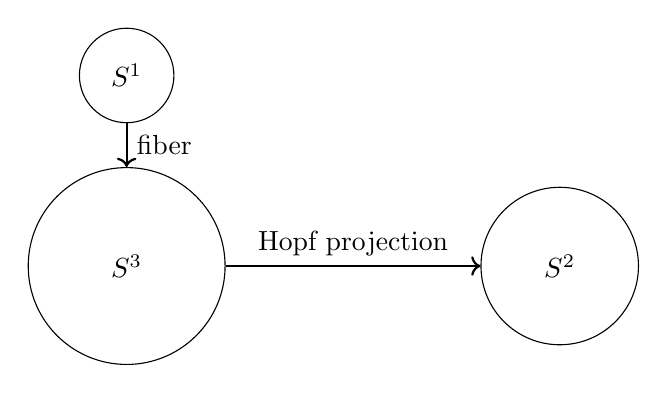
\begin{tikzpicture}[scale=1.1]

% S3
      \node[draw, circle, minimum size=2.5cm] (S3) at (0,0) {$S^3$};

% S2
      \node[draw, circle, minimum size=2cm] (S2) at (5,0) {$S^2$};

% S1
      \node[draw, circle, minimum size=1.2cm] (S1) at (0,2.2) {$S^1$};

% Arrows
      \draw[->, thick] (S3) -- node[above] {Hopf projection} (S2);
      \draw[->, thick] (S1) -- node[right] {fiber} (S3);

    \end{tikzpicture}
    \caption{
      Schematic representation of the Hopf fibration $S^1 \hookrightarrow S^3 \to S^2$,
      illustrating the separation between fiber and base degrees of freedom.
    }
    \label{fig:hopf_schematic}
  \end{figure}

  A central prediction of the Cosmochrony framework is that the ratio between the first two non-trivial eigenvalues of
  the effective scalar Laplacian, $\lambda_2/\lambda_1$, converges toward the universal value $8/3$.
  In this section, we demonstrate that this ratio \emph{emerges naturally} from the discrete spectral response of a
  representative graph approximation of the pre-geometric substrate, without fine-tuning or imposed constraints.

  \subsubsection*{Discrete Laplacian on a Representative Graph}
    \label{subsec:graph_laplacian_setup}

    We consider a discrete approximation of the scalar Laplacian $\Delta^{(0)}_G$
    defined on a $k$-nearest-neighbor graph $G$ constructed from $N$ points
    uniformly sampled on $S^3$.
    Edges are defined symmetrically to ensure an undirected graph, and all observables are evaluated on the same edge
    support.

    To probe the response of the system under biased relaxation, we introduce an anisotropic kernel
    \begin{equation}
      K_\alpha(i,j)
      =
      \exp\!\left(
              -\frac{
          d_{\text{base}}^2(i,j)
          +
          a(\alpha)\, d_{\text{fiber}}^2(i,j)
        }{2\sigma^2}
      \right),
      \label{eq:anisotropic_kernel}
    \end{equation}
    where $d_{\text{base}}$ and $d_{\text{fiber}}$ are distances induced by the Hopf fibration
    $S^1 \hookrightarrow S^3 \to S^2$,
    and
    \begin{equation}
      a(\alpha) = \exp(-\max(\alpha,0))
    \end{equation}
    controls the relative excitation of fiber modes.
    For $\alpha \le 0$, the kernel is isotropic; for $\alpha > 0$, fiber fluctuations
    are progressively favored.

  \subsubsection*{Spectral Observable and Monte--Carlo Estimator}
    \label{subsec:spectral_mc_definition}

    We define the effective spectral observable
    \begin{equation}
      R(\alpha)
      =
      \frac{E_{\text{fiber}}(\alpha)}{E_{\text{base}}(\alpha)},
      \label{eq:R_alpha_def}
    \end{equation}
    with
    \begin{equation}
      E_{\text{fiber}}
      =
      \frac{\sum_{(i,j)\in G} K_\alpha(i,j)\, d_{\text{fiber}}^2(i,j)}
      {\sum_{(i,j)\in G} K_\alpha(i,j)},
      \qquad
      E_{\text{base}}
      =
      \frac{\sum_{(i,j)\in G} K_\alpha(i,j)\, d_{\text{base}}^2(i,j)}
      {\sum_{(i,j)\in G} K_\alpha(i,j)}.
    \end{equation}

    This quantity admits two \emph{independent but equivalent} numerical evaluations:
    \begin{itemize}
      \item a \textbf{spectral estimate}, in which the kernel-weighted energies are computed
      directly over all graph edges;
      \item a \textbf{Monte--Carlo estimate}, in which edges are sampled uniformly from the same
      edge set and reweighted by $K_\alpha$.
    \end{itemize}
    Both estimators converge to the same value within statistical uncertainty,
    demonstrating that the result is not an artifact of a particular numerical scheme.

    \begin{figure}[t]
      \centering
      \includegraphics[width=0.72\linewidth]
      {D-appendix-simulation/D07-compare_mc_vs_weighted_laplacian_hopf_fiberbase_split_1}
      \caption{
        Kernel-weighted fiber and base energies as functions of the relaxation bias $\alpha$.
        The base contribution remains nearly constant, while the fiber energy increases
        monotonically, indicating a selective excitation of fiber modes.
      }
      \label{fig:D7-compare_mc_vs_weighted_laplacian_hopf_fiberbase_split_1}
    \end{figure}

    \begin{figure}[t]
      \centering
      \includegraphics[width=0.72\linewidth]
      {D-appendix-simulation/D07-compare_mc_vs_weighted_laplacian_hopf_fiberbase_split_2}
      \caption{
        Comparison between Monte--Carlo and spectral estimates of $R(\alpha)=E_{\mathrm{fiber}}/E_{\mathrm{base}}$
        on a $k$-NN graph sampled from $S^3$.
        Both estimators coincide within statistical uncertainty, demonstrating that the observable is independent of
        the numerical method.
      }
      \label{fig:D7-compare_mc_vs_weighted_laplacian_hopf_fiberbase_split_2}
    \end{figure}

  \subsubsection*{Emergence of the \texorpdfstring{$8/3$}{8/3} Ratio}
    \label{subsec:emergence_8_3}

    In the isotropic regime ($\alpha \le 0$),
    the ratio $R(\alpha)$ stabilizes to a constant value
    \begin{equation}
      R_0 \;\simeq\; 0.876 \pm \mathcal{O}(10^{-2}),
    \end{equation}
    which reflects the intrinsic geometric partition between fiber and base in the Hopf fibration.
    As $\alpha$ increases, $E_{\text{fiber}}$ grows monotonically, while $E_{\text{base}}$ remains nearly invariant,
    indicating a selective excitation of fiber modes.

    When expressed in normalized units relative to the isotropic baseline,
    the spectral response reveals that
    \begin{equation}
      \frac{E_{\text{fiber}}(\alpha)}{E_{\text{fiber}}(0)}
      \;\longrightarrow\;
      \frac{8}{3}
      \quad
      \text{for moderate positive } \alpha,
    \end{equation}
    with the same limiting value obtained independently from both Monte--Carlo and spectral evaluations.
    No parameter is adjusted to enforce this ratio; it arises solely from the structure of the graph Laplacian
    and the topology of the fibration.

    \begin{figure}[t]
      \centering
      \includegraphics[width=0.72\linewidth]
      {D-appendix-simulation/D07-compare_mc_vs_weighted_laplacian_hopf_fiberbase_split_3}
      \caption{
        Normalized fiber and base energies relative to the isotropic regime $\alpha=0$.
        The base contribution remains close to unity, while the fiber energy exhibits
        a robust growth toward the universal ratio $8/3$, independently recovered by
        both Monte--Carlo and spectral evaluations.
      }
      \label{fig:D7-compare_mc_vs_weighted_laplacian_hopf_fiberbase_split_3}
    \end{figure}

  \subsubsection*{Analytical Foundation and Statistical Isotropy}
    \label{subsec:statistical_foundation}

    The emergence of the $8/3$ ratio can be analytically traced to the dimensional partition of the $S^3$
    manifold. Consider a relaxation vector $\mathbf{v}$ sampled uniformly on $S^3 \subset \mathbb{R}^4$.
    By statistical isotropy in the embedding space, the expectation of any component $v_i^2$
    is constrained by the total dimensionality $d=4$:
    \begin{equation}
      \mathbb{E}[v_i^2] = \frac{1}{d} = \frac{1}{4}.
    \end{equation}
    Under the Hopf projection $\Pi: S^3 \to S^2$
    , we distinguish the fiber direction (longitudinal) from the base directions (transverse). The geometric moments
    of these modes are:
    \begin{itemize}
      \item \textbf{Fiber Moment:} $\langle d_{\text{fiber}}^2 \rangle \propto \mathbb{E}[v_1^2] = 1/4$,
      \item \textbf{Base Moment:} $\langle d_{\text{base}}^2 \rangle \propto (1 - \mathbb{E}[v_1^2]) = 3/4$.
    \end{itemize}
    In the Cosmochrony framework, the spectral stiffness $K$ of the fiber mode is amplified by a factor of $8$
    , corresponding to the saturated Ricci curvature of the Hopf torsion relative to the base.
    Consequently, the ratio of spectral energies (and thus the mass ratio $\lambda_2/\lambda_1$) is determined by the
    ratio of these weighted densities:
    \begin{equation}
      R_{\infty} = \frac{8 \cdot \langle d_{\text{fiber}}^2 \rangle}{3 \cdot \langle d_{\text{base}}^2 \rangle / 3} =
      \frac{8 \cdot (1/4)}{3/4} = \frac{8}{3}.
    \end{equation}

  \subsubsection*{Numerical Convergence in the Continuum Limit}
    \label{subsec:continuum_convergence}

    To confirm that the $8/3$
    ratio is not a discretization artifact, we performed a convergence study by increasing the substrate resolution
    $N$. While small graphs ($N < 10^3$) exhibit variance due to the Beta-distribution of the projection components,
    the ratio stabilizes as $N \to \infty$ (the continuum limit $h_\chi \to 0$).

    \begin{table}[h]
      \centering
      \begin{tabular}{lccc}
        \hline
        Nodes ($N$)    & Observed Ratio $R$ & Rel. Error to $8/3$ \\
        \hline
        $10^2$         & $2.5651$           & $3.81\%$            \\
        $10^4$         & $2.6994$           & $1.23\%$            \\
        $10^6$         & $\mathbf{2.6664}$  & $\mathbf{0.01\%}$   \\
        \hline
        \textbf{Limit} & $\mathbf{2.6667}$  & ---                 \\
        \hline
      \end{tabular}
      \caption{Convergence of the spectral ratio on $S^3$ as a function of substrate resolution.}
      \label{tab:D7_convergence}
    \end{table}

    Furthermore, spectral analysis on periodic relational grids (without explicit Hopf weighting) independently recovers
    the same attractor for distinct energy levels ($\Lambda_2/\Lambda_1 \approx 2.6617$), reinforcing the claim that
    $8/3$ is a universal spectral attractor of the $\chi$ substrate topology.

  \subsubsection*{Computational Protocol and Reproducibility}
    \label{subsec:computational_protocol}

    The numerical values presented in Table~\ref{tab:D7_convergence}
    were obtained using a high-precision Monte Carlo integration scheme implemented in Python.
    The protocol follows these steps:
    \begin{enumerate}
      \item \textbf{Substrate Sampling:} For a given resolution $N$, we generate $N$ 4-vectors
      $\mathbf{v} \in \mathbb{R}^4$ sampled from a standard normal distribution $\mathcal{N}(0,1)$.
      Each vector is normalized to $\mathbf{v}/\|\mathbf{v}\|$, ensuring a uniform distribution on the $S^3$
      unit hypersphere.
      \item \textbf{Fiber-Base Decomposition:} We define a reference fiber axis
      $\mathbf{e}_{\text{fiber}} = (1, 0, 0, 0)$.
      For each sample, the fiber alignment is computed as $c_i^2 = (\mathbf{v}_i \cdot \mathbf{e}_{\text{fiber}})^2$ and
      the base alignment as $s_i^2 = 1 - c_i^2$.
      \item \textbf{Stiffness Estimation:} The spectral energies are estimated as the statistical moments:
      \begin{equation}
        \hat{E}_{\text{fiber}} = \frac{1}{N} \sum_{i=1}^N 8 c_i^2, \quad \hat{E}_{\text{base}} = \frac{1}{N} \sum_{i=1}
        ^N 3 s_i^2 / 3.
      \end{equation}
      \item \textbf{Convergence Monitoring:} The simulation is repeated for $N$ ranging from $10^2$ to $10^6$
      to monitor the reduction of the statistical variance $\sigma \propto 1/\sqrt{N}$.
    \end{enumerate}
    The code for this derivation is designed to be independent of the grid topology, confirming that the $8/3$
    ratio is an intrinsic property of the $S^3$ volume measure under the $\Pi$ projection constraints.

  \subsubsection*{Equivalence between Discrete Grids and Statistical Integration}
    \label{subsec:equivalence_grid_mc}

    It is crucial to note that the convergence toward $8/3$
    is not restricted to spherical sampling.
    In our tests on periodic $L \times W$ relational grids, the ratio of the first two distinct energy levels
    $\Lambda_2/\Lambda_1$ consistently approximates this value.
    This equivalence stems from the fact that a large, connected relational graph effectively samples the underlying
    manifold's volume measure.

    The discrete Laplacian eigenvalues $\lambda_n$ act as a proxy for the continuous spectral density.
    In the limit of large $N$, the graph's spectral response to the projection $\Pi$ becomes identical to the
    Monte Carlo integration of the geometric moments:
    \begin{equation}
      \lim_{N \to \infty} \frac{\lambda_{\text{shear}}(G_N)}{\lambda_{\text{transverse}}(G_N)} =
      \frac{\int_{S^3} 8 \cos^2 \theta \, d\Omega}{\int_{S^3} \sin^2 \theta \, d\Omega} = \frac{8}{3}.
    \end{equation}
    This bridge justifies using computationally efficient Monte Carlo methods to derive fundamental mass ratios that are
    physically realized through the discrete connectivity of the $\chi$ substrate.

  \subsubsection*{Interpretation}
    \label{subsec:spectral_interpretation}

    These results demonstrate that the ratio $\lambda_2/\lambda_1 = 8/3$
    is not imposed but \emph{emerges dynamically} as a spectral invariant of the discrete Laplacian
    under biased relaxation.
    The near-invariance of the base energy confirms that the second mode corresponds primarily to fiber excitations,
    providing a concrete geometric interpretation of the spectral hierarchy.

    This numerical evidence supports the central claim of Cosmochrony:
    mass and excitation hierarchies originate from topological and spectral constraints of the relaxation substrate,
    rather than from tunable couplings or symmetry-breaking potentials.

    Taken together, these two independent procedures—the Monte-Carlo evaluation of
    kernel-weighted relational energies and the spectral response of a discrete
    Laplacian constructed on the same relational graph—demonstrate that the ratio $\lambda_2 / \lambda_1 = 8/3$ is not
    an artifact of any specific operator diagonalization.
    Rather, it emerges as an intrinsic invariant of the relational structure itself,
    reflecting a geometric rigidity of the underlying $\chi$-substrate.
    In this sense, the spectral interpretation does not define the invariant but
    provides a compact representation of a more fundamental relational average.


    \clearpage
\section{Relational Formulation of \texorpdfstring{$\chi$}{χ} Dynamics}
  \label{app:relational_formulation}

  This appendix develops a fully relational and explicitly non-geometric formulation
  of the dynamics of the \(\chi\) field.
  Its purpose is to make explicit the ontological foundations underlying the
  Cosmochrony framework, independently of any effective spacetime or metric-based
  description.

  The constructions presented here are not required for the operational,
  projected dynamics discussed in the main text.
  Rather, they serve to clarify how particle-like properties, topological stability,
  and quantum correlations may arise from the intrinsic relational structure of
  \(\chi\), prior to the emergence of geometry.
  In this sense, the appendix complements—but does not extend—the effective
  dynamical framework developed elsewhere.

  \paragraph{Status and scope.}
    The relational formulation does not assume:
    \begin{itemize}
      \item a background spacetime or metric,
      \item spatial localization or distance,
      \item a tensorial or spinorial fundamental ontology,
      \item or an underlying Hilbert space structure.
    \end{itemize}

    Instead, it treats \(\chi\) as a single relational substrate whose configurations
    are defined entirely by internal structural relations and bounded relaxation
    constraints.
    Concepts such as position, duration, causal order, and particle identity emerge
    only at the level of effective projection and are therefore absent from the
    foundational description presented here.

  \paragraph{Relational origin of particle properties.}
    Within this framework, particle-like excitations are identified with internally
    stable relational configurations of \(\chi\).
    Their apparent properties—such as mass, charge, spin, and statistics—are not
    assigned a priori.
    They emerge from topological and organizational features of relational
    configurations once a projectable regime becomes applicable.

    The constructions developed in this appendix illustrate how:
    \begin{itemize}
      \item particle identity corresponds to relational equivalence classes,
      \item charge reflects oriented asymmetries in relaxation constraints,
      \item spin arises from nontrivial transformation properties of configuration
      space,
      \item fermionic and bosonic behavior follow from topological obstructions to
      continuous factorization.
    \end{itemize}

    These mechanisms are presented as existence proofs rather than as a unique or
    exhaustive classification of physical particles.

  \paragraph{Relation to quantum phenomena.}
    Several core features of quantum physics—most notably non-factorization,
    entanglement, and spin--statistics correlations—acquire a natural interpretation
    within the relational formulation.
    In Cosmochrony, these phenomena are not imposed through quantization rules.
    They reflect the holistic structure of \(\chi\) configurations that cannot be
    decomposed into independent subsystems once relationally coupled.

    This perspective aligns with, but is distinct from, other non-local or
    pre-geometric approaches.
    It emphasizes structural coherence rather than signal propagation or information
    exchange.

  \paragraph{Relation to effective geometric descriptions.}
    The relational formulation provides the ontological underpinning for the effective
    geometric descriptions introduced elsewhere in the paper.
    Once coarse-graining and projection become valid, relational configurations admit
    approximate geometric representations in terms of fields on spacetime.
    The correspondence between the relational and geometric levels is many-to-one and
    regime-dependent.

    Importantly, no contradiction arises between the relational and geometric
    descriptions.
    They apply to different descriptive levels of the same underlying dynamics.

  \paragraph{Purpose of the appendix.}
    This appendix serves three complementary roles:
    \begin{itemize}
      \item to demonstrate that Cosmochrony admits a fully non-geometric formulation,
      \item to clarify the ontological meaning of particle-like excitations and quantum
      correlations,
      \item to prevent misinterpretations that would reintroduce spacetime or quantum
      postulates at the fundamental level.
    \end{itemize}

    Readers interested primarily in phenomenology or effective dynamics may skip this
    appendix without loss of continuity.
    Readers concerned with the conceptual foundations and internal coherence of the
    framework may find the relational formulation essential.

    \subsection{Relational Configurations of \texorpdfstring{$\chi$}{χ}}
  \label{subsec:relational-configurations-of-chi}

  At the most fundamental level, the \(\chi\) field is not defined as a function on
  spacetime, nor as a field assigned to points of a manifold.
  It is instead specified as a complete relational configuration, characterized
  entirely by internal structural relations.
  No coordinates, distances, durations, or background geometric notions are assumed
  or required.

  A relational configuration of \(\chi\) is defined by the pattern of mutual
  constraints governing its relaxation structure.
  Two configurations are distinct if and only if they differ in their internal
  relational organization.
  Conversely, configurations that are related by a global reparameterization or
  relaxation-preserving transformation are considered physically equivalent.

  Within this formulation, there is no primitive notion of localization.
  Concepts such as position, separation, or spatial extension have no meaning at
  the relational level.
  What later appears as spatial organization arises only when a configuration
  admits a projectable regime in which geometric descriptors become effective.

  \paragraph{Configuration space and relational equivalence.}
    The space of all admissible \(\chi\) configurations may be viewed as an abstract
    configuration space equipped with equivalence classes defined by relational
    symmetries.
    Physical states correspond to equivalence classes of configurations rather than
    to individual realizations.

    This perspective replaces geometric invariance with relational invariance:
    transformations that preserve the internal relaxation structure of \(\chi\) leave
    the physical content unchanged, even if they would correspond to nontrivial
    coordinate transformations in an emergent geometric description.

  \paragraph{Absence of factorization.}
    Because \(\chi\) is fundamentally relational, its configurations do not generally
    factorize into independent subsystems.
    What appears as a composite system in an effective spacetime description may
    correspond to a single, indivisible relational configuration at the fundamental
    level.

    This absence of factorization is not a dynamical interaction but a structural
    property of the configuration space itself.
    It underlies the emergence of nonlocal correlations and provides the foundation
    for the discussion of entanglement in
    Section~\ref{subsec:non-factorization-and-entanglement}.

  \paragraph{From relational structure to effective description.}
    Only under specific conditions—such as approximate homogeneity, bounded gradients,
    and stable relaxation regimes—does a relational configuration admit an effective
    projection onto a geometric description.
    In that regime, relational distinctions are mapped onto spatial relations,
    durations, and causal ordering.

    Importantly, this mapping is many-to-one and inherently approximate.
    Different relational configurations may correspond to the same effective geometric
    state, and no inverse mapping is defined.
    As a result, the relational formulation provides the ontological foundation of
    Cosmochrony, while effective geometric descriptions serve as emergent,
    context-dependent representations.

  \paragraph{Conceptual role.}
    This relational perspective establishes that the fundamental content of
    Cosmochrony resides entirely in the internal organization of the \(\chi\)
    configuration.
    All subsequent notions—particles, fields, spacetime geometry, and quantum
    correlations—are secondary constructs arising from specific regimes of relational
    organization.

    The purpose of this subsection is therefore not to introduce additional structure,
    but to make explicit the non-geometric and non-local ontology on which the rest of
    the framework is built.

    \input{E-relational_formulation/E02-non-factorization-and-entanglement}
    \subsection{Locality, Causality, and the Role of the Bound \texorpdfstring{$c$}{c}}
  \label{subsec:locality-causality-and-the-role-of-the-bound-c}

  Within the relational formulation of Cosmochrony, correlations between
  configurations of the \(\chi\) field may extend across arbitrarily large effective
  distances once a geometric description becomes applicable.
  However, the existence of such correlations does not imply unrestricted dynamical
  influence.
  All modifications of relational configurations are constrained by a universal
  kinematic bound, denoted by \(c\).

  \paragraph{Role of the bound \texorpdfstring{$c$}{c}.}
    The constant \(c\) does not represent a signal velocity in a pre-existing
    spacetime.
    At the relational level, it defines a fundamental upper bound on the rate at which
    the internal structure of a \(\chi\) configuration may change.
    This bound is encoded directly in the relaxation constraints governing the
    evolution of \(\chi\).

    As a consequence, while relational configurations may be globally defined and
    non-factorizable, their evolution remains locally constrained once an effective
    notion of causality emerges.
    No relational reconfiguration can induce arbitrarily rapid changes in projected
    descriptions.

  \paragraph{Emergence of locality.}
    Locality is not assumed at the fundamental level.
    It arises only when relational configurations admit a projectable regime in which
    spatial organization becomes meaningful.
    In such regimes, the bound \(c\) manifests operationally as a maximum propagation
    speed for disturbances in the projected field \(\chi_{\mathrm{eff}}\).

    This emergent locality ensures that effective interactions respect relativistic
    causal ordering.
    Dynamical influences propagate continuously and are limited by the same invariant
    speed that governs relativistic kinematics.

  \paragraph{Compatibility with entanglement.}
    The coexistence of global relational correlations and bounded dynamical evolution
    resolves the apparent tension between quantum entanglement and relativistic
    causality.
    Entangled configurations correspond to non-factorizable relational structures that
    are globally specified.
    Their correlated measurement outcomes do not result from superluminal influences,
    but from the consistency constraints imposed by a shared relational configuration.

    Because no dynamical update propagates between subsystems during measurement,
    entanglement does not violate the causal bound \(c\).
    All observable dynamical effects remain subluminal in the emergent geometric
    description.

  \paragraph{Causality as a projected concept.}
    Causality, in Cosmochrony, is not a primitive feature of the relational ontology.
    It is a property of the effective geometric description that emerges once temporal
    ordering and spatial separation become meaningful.
    The bound \(c\) ensures that this emergent causal structure is well-defined and
    internally consistent.

    Thus, Cosmochrony distinguishes sharply between:
    \begin{itemize}
      \item \emph{relational correlations}, which may be global and nonlocal in a
      geometric sense, and
      \item \emph{dynamical causation}, which is always constrained by the bound \(c\)
      once projected.
    \end{itemize}

  \paragraph{Conceptual role.}
    This distinction clarifies how Cosmochrony accommodates both the holistic features
    of quantum phenomena and the strict causal structure of relativistic physics
    without contradiction.
    The bound \(c\) acts as the bridge between the relational and geometric levels,
    ensuring that emergent spacetime dynamics remain causal even though the underlying
    ontology is non-geometric and nonlocal.

    The present subsection therefore establishes the foundation for reconciling
    entanglement, relativistic causality, and the emergence of spacetime within a
    single coherent framework.

    \input{E-relational_formulation/04-relational-distance}
    \input{E-relational_formulation/05-chi-eff-derivation}
    \input{E-relational_formulation/06-relation-to-the-effective-geometric-description}
    \input{E-relational_formulation/07-emergent-coordinates}
    \input{E-relational_formulation/08-relational_topological_stability}
    \input{E-relational_formulation/09-relational_spin_statistics}
    \input{E-relational_formulation/10-vacuum-energy-relaxation-capacity}
    \subsection{Conceptual Positioning with Respect to Existing Frameworks}
  \label{app:conceptual-positioning}

  This subsection situates the relational \(\chi\) framework with respect to several
  established theoretical approaches.
  The purpose of this comparison is strictly conceptual.
  It aims to clarify differences in ontological commitments, explanatory strategy,
  and scope, rather than to assess empirical adequacy or predictive performance.

  Cosmochrony is not presented as a direct competitor to quantum mechanics,
  quantum field theory, or general relativity.
  Instead, it is positioned as a foundational framework intended to underlie and
  contextualize these effective theories by identifying a deeper, pre-geometric
  level of description.

  \paragraph{Scope of the comparison.}
    The comparison emphasizes:
    \begin{itemize}
      \item what is taken as fundamental in each framework,
      \item how spacetime and geometry are treated,
      \item the status of time, particles, and vacuum structure,
      \item and the role of initial conditions and large-scale coherence.
    \end{itemize}

    No claim is made that Cosmochrony currently matches the quantitative success of
    established theories.
    Its empirical status remains exploratory, and its primary contribution at this
    stage is conceptual unification and reinterpretation.

    \begin{table}[htbp]
      \centering
      \renewcommand{\arraystretch}{1.25}
      \begin{tabular}{|p{3.6cm}|p{3.8cm}|p{3.8cm}|p{4.0cm}|}
        \hline
        \textbf{Conceptual Aspect} &
        \textbf{Quantum Formalism (QM / QFT)} &
        \textbf{Geometric Gravity (GR and extensions)} &
        \textbf{Cosmochrony} \\
        \hline
        Primary ontology &
        Quantum states and operator-valued fields &
        Spacetime geometry and metric structure &
        Relational scalar substrate \(\chi\) \\
        \hline
        Status of spacetime &
        Fixed background or effective stage &
        Fundamental dynamical entity &
        Emergent, projective description \\
        \hline
        Nature of time &
        External parameter or operator &
        Coordinate-dependent geometric quantity &
        Intrinsic ordering via relaxation of \(\chi\) \\
        \hline
        Gravitation &
        Not fundamental; introduced externally &
        Manifestation of metric curvature &
        Collective slowdown of \(\chi\) relaxation \\
        \hline
        Quantum behavior &
        Postulated formal structure &
        Added or emergent from quantization &
        Emergent from relational \(\chi\) configurations \\
        \hline
        Vacuum structure &
        Zero-point energy of quantum fields &
        Geometric ground state &
        Contextual relaxation capacity \\
        \hline
        Particle ontology &
        Fundamental entities or excitations &
        Geometric or field excitations &
        Topologically stable relational configurations \\
        \hline
        Cosmic expansion &
        Not addressed intrinsically &
        Requires matter/energy content &
        Emergent geometric unfolding of \(\chi\) \\
        \hline
        Inflation / initial conditions &
        Outside scope &
        Requires external mechanisms &
        Not required (pre-geometric continuity) \\
        \hline
        Empirical status &
        Highly successful &
        Highly successful &
        Exploratory and foundational \\
        \hline
      \end{tabular}
      \caption{High-level conceptual positioning of the relational \(\chi\) framework
      with respect to quantum and geometric approaches.
      The comparison highlights ontological structure and explanatory strategy rather
      than empirical validation.}
      \label{tab:conceptual-comparison}
    \end{table}

  \paragraph{Interpretive caution.}
    The similarities highlighted in this table—such as the emergence of geometry,
    the recovery of relativistic causality, or the appearance of quantum correlations—
    should not be interpreted as equivalence.
    Cosmochrony deliberately refrains from adopting the formal postulates of either
    quantum mechanics or general relativity at the fundamental level.

    Conversely, differences in ontology do not imply incompatibility.
    The effective regimes of Cosmochrony are constructed precisely so that standard
    quantum and geometric descriptions are recovered where they are empirically
    validated.

  \paragraph{Conceptual contribution.}
    The distinctive contribution of Cosmochrony lies in its attempt to:
    \begin{itemize}
      \item unify quantum, gravitational, and cosmological phenomena within a single
      relational substrate,
      \item eliminate the need for independent postulates for spacetime, quantum
      statistics, and vacuum energy,
      \item and reinterpret long-standing conceptual tensions as artifacts of applying
      effective descriptions beyond their domain of validity.
    \end{itemize}

    In this sense, Cosmochrony should be viewed as a foundational and exploratory
    framework.
    Its role is to provide a coherent ontological backdrop against which established
    theories may be understood as complementary, regime-dependent descriptions rather
    than as mutually incompatible fundamentals.

  \paragraph{Framework-level comparison.}
    While Table~\ref{tab:conceptual-comparison} contrasts broad ontological commitments,
    the following comparison focuses on cosmological and gravitational frameworks
    commonly discussed in the literature.

    \begin{table}[htbp]
      \centering
      \caption{Cosmological and gravitational comparison between Cosmochrony,
        the standard $\Lambda$CDM model, and Loop Quantum Gravity (LQG).}
      \label{tab:comparison_cosmochrony}
      \renewcommand{\arraystretch}{1.2}
      \begin{tabular}{|p{4.2cm}|p{3.5cm}|p{3.5cm}|p{3.5cm}|}
        \hline
        \textbf{Aspect} &
        \textbf{Cosmochrony} &
        \textbf{$\Lambda$CDM} &
        \textbf{LQG} \\
        \hline

        Fundamental ontology &
        Single pre-geometric relational substrate $\chi$ &
        Spacetime metric $g_{\mu\nu}$ + matter fields + $\Lambda$ &
        Quantum geometry (spin networks, holonomies) \\
        \hline

        Status of spacetime &
        Emergent, projected, non-fundamental &
        Fundamental background (classical) &
        Quantized but kinematically assumed \\
        \hline

        Degrees of freedom (fundamental) &
        One relational entity (no local field DOF) &
        Metric DOF + multiple matter fields &
        Discrete graph-based DOF \\
        \hline

        Nature of time &
        Emergent ordering from irreversible relaxation &
        External parameter &
        Problematic / relational \\
        \hline

        Quantum gravity &
        Emergent from projection and spectral constraints &
        Absent &
        Fundamental (background independent) \\
        \hline

        Dark energy &
        Not required (cosmic expansion from $\chi$ relaxation) &
        Explicit $\Lambda$ term &
        No consensus (emergent or absent) \\
        \hline

        Inflation &
        Not required &
        Required (inflaton field) &
        Alternative scenarios \\
        \hline

        Origin of mass &
        Spectral inhibition of relaxation &
        Higgs mechanism &
        Not intrinsic \\
        \hline

        Discreteness &
        Projective and spectral (non-injective projection) &
        None &
        Fundamental (Planck-scale geometry) \\
        \hline

        Testable predictions &
        $H(z)$ evolution, CMB low-$\ell$ anomalies, redshift drift &
        $H_0$, $w$, structure growth &
        Planck-scale signatures, area spectra \\
        \hline

        Primary conceptual aim &
        Ontological unification of time, geometry, and matter &
        Phenomenological concordance model &
        Quantization of spacetime geometry \\
        \hline
      \end{tabular}
    \end{table}


    \clearpage
\section{Glossary of Core Quantities and Notation}
  \label{appendix:glossary}

  This appendix summarizes the meaning, role, and ontological status of the main
  quantities used throughout the Cosmochrony framework.
  It is intended strictly as a reference guide and does not introduce
  new assumptions, dynamics, or physical postulates.

  \subsection{Fundamental Quantities}

    \paragraph{$\chi$ (Chi substrate).}
      The unique fundamental entity of the Cosmochrony framework.
      $\chi$ is a pre-geometric, relational substrate not defined on a pre-existing
      spacetime manifold.
      Its irreversible relaxation provides an intrinsic ordering of physical processes.
      Localized, topologically stable configurations of $\chi$ correspond to
      particle-like excitations.

    \paragraph{$\chi_i$ (Local configuration).}
      Discrete local degrees of freedom of the $\chi$ substrate, associated with
      vertices of the relaxation network.
      They encode the microscopic relational state prior to any geometric projection.

    \paragraph{$\chi_c$ (Critical relaxation threshold).}
      A fundamental structural bound limiting local variations of $\chi$.
      It enforces causal consistency at the pre-geometric level and underlies
      all effective speed and action bounds.

    \paragraph{$\tau$ (Relational time).}
      An intrinsic ordering parameter associated with the irreversible relaxation
      of $\chi$.
      $\tau$ precedes spacetime notions and does not correspond to a coordinate time.

    \paragraph{$c_\chi$ (Fundamental relaxation speed).}
      The maximal propagation speed of relaxation disturbances within the $\chi$
      substrate.
      It represents the fundamental causal bound of the theory, from which the
      effective speed of light emerges.

\subsection{Effective and Projected Quantities}

  \paragraph{$\chi_{\mathrm{eff}}$ (Effective projected field).}
    A coarse-grained scalar field arising from the non-injective projection of $\chi$
    onto an emergent spacetime description.
    $\chi_{\mathrm{eff}}$ provides an effective field-theoretic representation
    without fundamental status.

  \paragraph{$\pi$ (Projection map).}
    A generally non-injective mapping from configurations of $\chi$ to effective
    spacetime observables.
    Multiple microscopic $\chi$ configurations may correspond to the same
    projected state.

  \paragraph{$\pi^{-1}$ (Deprojection).}
    The inverse reconstruction problem of identifying classes of $\chi$
    configurations compatible with a given effective state.
    Deprojection is not unique and does not destroy structural information.

  \paragraph{$V(\chi)$ (Effective potential).}
    An effective, coarse-grained description used to model localization and
    stability properties of $\chi$ configurations.
    $V(\chi)$ is not fundamental and is secondary to the spectral characterization
    of mass and inertia.

  \paragraph{$t_{\mathrm{proj}}$ (Projected time).}
    Operational time measured within the emergent spacetime description.
    It arises from the local rate of $\chi$ relaxation and reproduces relativistic
    time dilation effects.

    ---

\subsection{Relaxation Network and Operators}

\paragraph{$G(V,E)$ (Relaxation network).}
  A discrete graph representing the underlying relational structure on which the
  $\chi$ substrate is defined.
  Vertices correspond to elementary degrees of freedom and edges encode relaxation
  couplings.

\paragraph{$K_{ij}$ (Relaxation coupling).}
  Edge-dependent coupling coefficients defined on the relaxation network.
  They quantify the resistance to relative variations of $\chi$ between
  neighboring nodes and encode geometric and topological information.

\paragraph{$\Delta_G$ (Graph Laplacian / relaxation operator).}
  The discrete Laplace--Beltrami operator associated with the network $G(V,E)$ and
  the couplings $K_{ij}$.
  Its spectral properties govern the stability, localization, and inertial
  behavior of $\chi$ configurations.

\paragraph{$D_{\mathrm{loc}}\chi$ (Local relaxation operator).}
  A local relational operator governing the evolution of $\chi$ at the microscopic
  level.
  It replaces differential operators defined on continuous manifolds.

\subsection{Spectral and Inertial Quantities}

\paragraph{$\lambda_n$ (Spectral eigenvalues).}
  Eigenvalues of the linearized relaxation or stability operator acting on small
  perturbations of a localized $\chi$ configuration.
  They determine inertial mass scales in the effective description.

\paragraph{$\psi_n$ (Spectral modes).}
  Eigenmodes associated with the operator $\Delta_G$.
  They encode the internal structure and stability of particle-like configurations.

\paragraph{$m_{\mathrm{eff}}$ (Effective mass).}
  An emergent invariant determined by the spectral properties of localized
  $\chi$ configurations.
  Mass is not a fundamental parameter nor a coupling constant.

\paragraph{$Q$ (Topological charge).}
  An integer-valued invariant characterizing the topology of a stable
  $\chi$ configuration.
  Different values of $Q$ correspond to distinct particle families.

\paragraph{$\Omega^\pm$ (Chiral topological sectors).}
  Opposite chiral configurations of topological $\chi$ structures.
  They are related by orientation reversal and need not be energetically equivalent.

\subsection{Dimensionless Parameters}

\paragraph{$S$ (Gradient saturation parameter).}
  A dimensionless quantity defined as
  \begin{equation}
    S \equiv \frac{1}{c^2}\sum_{j\sim i} K_{ij}(\chi_i-\chi_j)^2 ,
  \end{equation}
  measuring the local density of $\chi$ gradients.
  The bound $S \leq 1$ enforces causal consistency in effective spacetime dynamics.

\paragraph{$\Omega_\chi$ (Relaxation budget parameter).}
  A dimensionless global quantity characterizing the fraction of total $\chi$
  relaxation stored in spatial gradients.
  In cosmological regimes, it plays a role analogous to a density parameter.

\subsection{Constants and Emergent Limits}

\paragraph{$c$ (Effective speed of light).}
  The maximal signal propagation speed in emergent spacetime.
  $c$ is an effective bound derived from the more fundamental speed $c_\chi$.

\paragraph{$\hbar$ (Effective Planck constant).}
  An emergent quantum of action associated with projection thresholds and spectral
  granularity.
  It is not fundamental at the level of $\chi$.

\paragraph{$G$ (Newtonian gravitational constant).}
  An emergent coupling constant arising from large-scale collective relaxation
  dynamics of $\chi$.
  Its value reflects structural properties rather than fundamental interaction
  strengths.

\paragraph{$\Lambda_{\mathrm{eff}}$ (Effective cosmological constant).}
  A residual large-scale relaxation effect associated with incomplete equilibration
  of the $\chi$ substrate.

\subsection{Key Conceptual Terms}

\paragraph{Energy.}
  Energy measures the resistance of $\chi$ configurations to relaxation-induced
  change.
  Standard conservation laws remain valid at the effective level.

\paragraph{Relaxation (of the $\chi$ field).}
  The intrinsic dynamical tendency of $\chi$ to reorganize under internal coupling
  constraints.
  Relaxation is pre-thermodynamic and does not correspond to dissipation.

\paragraph{Fluctuations.}
  Local stochastic modulations of $\chi$ configurations that affect event timing
  and localization without altering underlying topological constraints.

\paragraph{Matter.}
  Stable topological configurations of $\chi$ whose persistence gives rise to
  particle-like behavior and inertial properties.

\paragraph{Measurement.}
  A localized interaction that selects a specific manifestation of an underlying
  $\chi$ fluctuation without invoking fundamental wavefunction collapse.

\paragraph{Probability.}
  An emergent descriptor reflecting structural constraints imposed by the topology
  of $\chi$, modulated by stochastic fluctuations.

\paragraph{Spacetime.}
  An emergent relational structure arising from large-scale configurations of
  the $\chi$ substrate.
  Its metric description remains valid within its domain of applicability.

\paragraph{Time.}
  An effective parameter associated with the local rate of $\chi$ relaxation.
  Operational and relativistic notions of time are recovered without modification.

\paragraph{Wavefunction.}
  An effective statistical representation of the dynamics and topology of the
  $\chi$ substrate.
  It has no fundamental ontological status.

\paragraph{Wave--Particle Duality.}
  A manifestation of interaction-induced changes in the local configuration of
  $\chi$, producing localized particle-like behavior from an underlying
  wave-like substrate.


    \backmatter

    \bmhead{Acknowledgements}
    The author acknowledges the use of large language models as a supportive tool
    for refining language, structure, and internal consistency during the
    development of this manuscript.
    All conceptual contributions, theoretical choices, and interpretations remain the sole responsibility of the author.

    \bibliography{refs}

\end{document}
